\documentclass[twoside]{book}

% Packages required by doxygen
\usepackage{fixltx2e}
\usepackage{calc}
\usepackage{doxygen}
\usepackage{graphicx}
\usepackage[utf8]{inputenc}
\usepackage{makeidx}
\usepackage{multicol}
\usepackage{multirow}
\PassOptionsToPackage{warn}{textcomp}
\usepackage{textcomp}
\usepackage[nointegrals]{wasysym}
\usepackage[table]{xcolor}

% Font selection
\usepackage[T1]{fontenc}
\usepackage{mathptmx}
\usepackage[scaled=.90]{helvet}
\usepackage{courier}
\usepackage{amssymb}
\usepackage{sectsty}
\renewcommand{\familydefault}{\sfdefault}
\allsectionsfont{%
  \fontseries{bc}\selectfont%
  \color{darkgray}%
}
\renewcommand{\DoxyLabelFont}{%
  \fontseries{bc}\selectfont%
  \color{darkgray}%
}
\newcommand{\+}{\discretionary{\mbox{\scriptsize$\hookleftarrow$}}{}{}}

% Page & text layout
\usepackage{geometry}
\geometry{%
  a4paper,%
  top=2.5cm,%
  bottom=2.5cm,%
  left=2.5cm,%
  right=2.5cm%
}
\tolerance=750
\hfuzz=15pt
\hbadness=750
\setlength{\emergencystretch}{15pt}
\setlength{\parindent}{0cm}
\setlength{\parskip}{0.2cm}
\makeatletter
\renewcommand{\paragraph}{%
  \@startsection{paragraph}{4}{0ex}{-1.0ex}{1.0ex}{%
    \normalfont\normalsize\bfseries\SS@parafont%
  }%
}
\renewcommand{\subparagraph}{%
  \@startsection{subparagraph}{5}{0ex}{-1.0ex}{1.0ex}{%
    \normalfont\normalsize\bfseries\SS@subparafont%
  }%
}
\makeatother

% Headers & footers
\usepackage{fancyhdr}
\pagestyle{fancyplain}
\fancyhead[LE]{\fancyplain{}{\bfseries\thepage}}
\fancyhead[CE]{\fancyplain{}{}}
\fancyhead[RE]{\fancyplain{}{\bfseries\leftmark}}
\fancyhead[LO]{\fancyplain{}{\bfseries\rightmark}}
\fancyhead[CO]{\fancyplain{}{}}
\fancyhead[RO]{\fancyplain{}{\bfseries\thepage}}
\fancyfoot[LE]{\fancyplain{}{}}
\fancyfoot[CE]{\fancyplain{}{}}
\fancyfoot[RE]{\fancyplain{}{\bfseries\scriptsize Generated on Tue Mar 17 2015 13\+:29\+:45 for Gem Illuminator by Doxygen }}
\fancyfoot[LO]{\fancyplain{}{\bfseries\scriptsize Generated on Tue Mar 17 2015 13\+:29\+:45 for Gem Illuminator by Doxygen }}
\fancyfoot[CO]{\fancyplain{}{}}
\fancyfoot[RO]{\fancyplain{}{}}
\renewcommand{\footrulewidth}{0.4pt}
\renewcommand{\chaptermark}[1]{%
  \markboth{#1}{}%
}
\renewcommand{\sectionmark}[1]{%
  \markright{\thesection\ #1}%
}

% Indices & bibliography
\usepackage{natbib}
\usepackage[titles]{tocloft}
\setcounter{tocdepth}{3}
\setcounter{secnumdepth}{5}
\makeindex

% Hyperlinks (required, but should be loaded last)
\usepackage{ifpdf}
\ifpdf
  \usepackage[pdftex,pagebackref=true]{hyperref}
\else
  \usepackage[ps2pdf,pagebackref=true]{hyperref}
\fi
\hypersetup{%
  colorlinks=true,%
  linkcolor=blue,%
  citecolor=blue,%
  unicode%
}

% Custom commands
\newcommand{\clearemptydoublepage}{%
  \newpage{\pagestyle{empty}\cleardoublepage}%
}


%===== C O N T E N T S =====

\begin{document}

% Titlepage & ToC
\hypersetup{pageanchor=false,
             bookmarks=true,
             bookmarksnumbered=true,
             pdfencoding=unicode
            }
\pagenumbering{roman}
\begin{titlepage}
\vspace*{7cm}
\begin{center}%
{\Large Gem Illuminator }\\
\vspace*{1cm}
{\large Generated by Doxygen 1.8.8}\\
\vspace*{0.5cm}
{\small Tue Mar 17 2015 13:29:45}\\
\end{center}
\end{titlepage}
\clearemptydoublepage
\tableofcontents
\clearemptydoublepage
\pagenumbering{arabic}
\hypersetup{pageanchor=true}

%--- Begin generated contents ---
\chapter{Namespace Index}
\section{Namespace List}
Here is a list of all namespaces with brief descriptions\+:\begin{DoxyCompactList}
\item\contentsline{section}{\hyperlink{namespaceorg}{org} }{\pageref{namespaceorg}}{}
\item\contentsline{section}{\hyperlink{namespaceorg_1_1qtproject}{org.\+qtproject} }{\pageref{namespaceorg_1_1qtproject}}{}
\item\contentsline{section}{\hyperlink{namespaceorg_1_1qtproject_1_1qt5}{org.\+qtproject.\+qt5} }{\pageref{namespaceorg_1_1qtproject_1_1qt5}}{}
\item\contentsline{section}{\hyperlink{namespaceorg_1_1qtproject_1_1qt5_1_1android}{org.\+qtproject.\+qt5.\+android} }{\pageref{namespaceorg_1_1qtproject_1_1qt5_1_1android}}{}
\item\contentsline{section}{\hyperlink{namespaceorg_1_1qtproject_1_1qt5_1_1android_1_1bindings}{org.\+qtproject.\+qt5.\+android.\+bindings} }{\pageref{namespaceorg_1_1qtproject_1_1qt5_1_1android_1_1bindings}}{}
\end{DoxyCompactList}

\chapter{Hierarchical Index}
\section{Class Hierarchy}
This inheritance list is sorted roughly, but not completely, alphabetically\+:\begin{DoxyCompactList}
\item \contentsline{section}{Gem\+Data}{\pageref{class_gem_data}}{}
\item \contentsline{section}{Gem\+Renderer}{\pageref{class_gem_renderer}}{}
\item \contentsline{section}{Light\+Ray\+Data}{\pageref{class_light_ray_data}}{}
\item \contentsline{section}{Q\+Hash$<$ Key, T $>$}{\pageref{class_q_hash}}{}
\item \contentsline{section}{Q\+Hash$<$ Abstract\+Gem $\ast$, Gem\+Data\+Info $\ast$ $>$}{\pageref{class_q_hash}}{}
\item \contentsline{section}{Q\+Hash$<$ Gem\+Type, Gem\+Render\+Data $\ast$ $>$}{\pageref{class_q_hash}}{}
\item \contentsline{section}{Q\+Hash$<$ Gem\+Type, Q\+List$<$ Q\+Open\+G\+L\+Buffer $\ast$ $>$ $\ast$ $>$}{\pageref{class_q_hash}}{}
\item \contentsline{section}{Q\+Hash$<$ Q\+Open\+G\+L\+Buffer $\ast$, Q\+List$<$ Gem\+Data\+Info $\ast$ $>$ $\ast$ $>$}{\pageref{class_q_hash}}{}
\item \contentsline{section}{Q\+List$<$ T $>$}{\pageref{class_q_list}}{}
\item \contentsline{section}{Q\+List$<$ Abstract\+Gem $\ast$ $>$}{\pageref{class_q_list}}{}
\item \contentsline{section}{Q\+List$<$ Gem\+Data\+Info $\ast$ $>$}{\pageref{class_q_list}}{}
\item \contentsline{section}{Q\+List$<$ Light\+Ray $\ast$ $>$}{\pageref{class_q_list}}{}
\item \contentsline{section}{Q\+List$<$ Triangle $\ast$ $>$}{\pageref{class_q_list}}{}
\item Q\+Object\begin{DoxyCompactList}
\item \contentsline{section}{Abstract\+Gem}{\pageref{class_abstract_gem}}{}
\begin{DoxyCompactList}
\item \contentsline{section}{Cube\+Gem}{\pageref{class_cube_gem}}{}
\item \contentsline{section}{Scene\+Bounds}{\pageref{class_scene_bounds}}{}
\item \contentsline{section}{Tetrahedron\+Gem}{\pageref{class_tetrahedron_gem}}{}
\end{DoxyCompactList}
\item \contentsline{section}{Camera}{\pageref{class_camera}}{}
\item \contentsline{section}{Config}{\pageref{class_config}}{}
\item \contentsline{section}{Light\+Ray}{\pageref{class_light_ray}}{}
\item \contentsline{section}{Light\+Ray\+Renderer}{\pageref{class_light_ray_renderer}}{}
\item \contentsline{section}{Navigation}{\pageref{class_navigation}}{}
\item \contentsline{section}{Painter}{\pageref{class_painter}}{}
\item \contentsline{section}{Player}{\pageref{class_player}}{}
\item \contentsline{section}{Scene\+Renderer}{\pageref{class_scene_renderer}}{}
\end{DoxyCompactList}
\item Q\+Quick\+Item\begin{DoxyCompactList}
\item \contentsline{section}{Painter\+Q\+M\+L}{\pageref{class_painter_q_m_l}}{}
\item \contentsline{section}{Scene}{\pageref{class_scene}}{}
\end{DoxyCompactList}
\item \contentsline{section}{Q\+Set$<$ T $>$}{\pageref{class_q_set}}{}
\item \contentsline{section}{Q\+Set$<$ Light\+Ray\+Data $>$}{\pageref{class_q_set}}{}
\item \contentsline{section}{Q\+Vector$<$ T $>$}{\pageref{class_q_vector}}{}
\item \contentsline{section}{Q\+Vector$<$ Light\+Ray\+Data $>$}{\pageref{class_q_vector}}{}
\item \contentsline{section}{Screen\+Aligned\+Quad}{\pageref{class_screen_aligned_quad}}{}
\item \contentsline{section}{Triangle}{\pageref{class_triangle}}{}
\end{DoxyCompactList}

\chapter{Class Index}
\section{Class List}
Here are the classes, structs, unions and interfaces with brief descriptions\+:\begin{DoxyCompactList}
\item\contentsline{section}{\hyperlink{class_abstract_gem}{Abstract\+Gem} }{\pageref{class_abstract_gem}}{}
\item\contentsline{section}{\hyperlink{class_camera}{Camera} }{\pageref{class_camera}}{}
\item\contentsline{section}{\hyperlink{class_config}{Config} }{\pageref{class_config}}{}
\item\contentsline{section}{\hyperlink{class_cube_gem}{Cube\+Gem} }{\pageref{class_cube_gem}}{}
\item\contentsline{section}{\hyperlink{class_gem_data}{Gem\+Data} }{\pageref{class_gem_data}}{}
\item\contentsline{section}{\hyperlink{class_gem_renderer}{Gem\+Renderer} }{\pageref{class_gem_renderer}}{}
\item\contentsline{section}{\hyperlink{class_light_ray}{Light\+Ray} }{\pageref{class_light_ray}}{}
\item\contentsline{section}{\hyperlink{class_light_ray_data}{Light\+Ray\+Data} \\*Stores data of a \hyperlink{class_light_ray}{Light\+Ray}. The \hyperlink{class_light_ray_data}{Light\+Ray\+Data} doesn\textquotesingle{}t inherit from Q\+Object, so it can be stored in Qt-\/\+Containers (currently only those require == or q\+Hash) by Value }{\pageref{class_light_ray_data}}{}
\item\contentsline{section}{\hyperlink{class_light_ray_renderer}{Light\+Ray\+Renderer} }{\pageref{class_light_ray_renderer}}{}
\item\contentsline{section}{\hyperlink{class_navigation}{Navigation} }{\pageref{class_navigation}}{}
\item\contentsline{section}{\hyperlink{class_painter}{Painter} \\*The \hyperlink{class_painter}{Painter} class  Includes the rendering process, thus creates the whole picture }{\pageref{class_painter}}{}
\item\contentsline{section}{\hyperlink{class_painter_q_m_l}{Painter\+Q\+M\+L} }{\pageref{class_painter_q_m_l}}{}
\item\contentsline{section}{\hyperlink{class_player}{Player} }{\pageref{class_player}}{}
\item\contentsline{section}{\hyperlink{class_q_hash}{Q\+Hash$<$ Key, T $>$} }{\pageref{class_q_hash}}{}
\item\contentsline{section}{\hyperlink{class_q_list}{Q\+List$<$ T $>$} }{\pageref{class_q_list}}{}
\item\contentsline{section}{\hyperlink{class_q_set}{Q\+Set$<$ T $>$} }{\pageref{class_q_set}}{}
\item\contentsline{section}{\hyperlink{class_q_vector}{Q\+Vector$<$ T $>$} }{\pageref{class_q_vector}}{}
\item\contentsline{section}{\hyperlink{class_scene}{Scene} }{\pageref{class_scene}}{}
\item\contentsline{section}{\hyperlink{class_scene_bounds}{Scene\+Bounds} }{\pageref{class_scene_bounds}}{}
\item\contentsline{section}{\hyperlink{class_scene_renderer}{Scene\+Renderer} \\*The \hyperlink{class_scene_renderer}{Scene\+Renderer} class  Renders the scene\+: Packs the scene in the buffer and draws the scene in one call }{\pageref{class_scene_renderer}}{}
\item\contentsline{section}{\hyperlink{class_screen_aligned_quad}{Screen\+Aligned\+Quad} }{\pageref{class_screen_aligned_quad}}{}
\item\contentsline{section}{\hyperlink{class_tetrahedron_gem}{Tetrahedron\+Gem} }{\pageref{class_tetrahedron_gem}}{}
\item\contentsline{section}{\hyperlink{class_triangle}{Triangle} }{\pageref{class_triangle}}{}
\end{DoxyCompactList}

\chapter{File Index}
\section{File List}
Here is a list of all files with brief descriptions\+:\begin{DoxyCompactList}
\item\contentsline{section}{\hyperlink{abstractgem_8cpp}{abstractgem.\+cpp} }{\pageref{abstractgem_8cpp}}{}
\item\contentsline{section}{\hyperlink{abstractgem_8h}{abstractgem.\+h} }{\pageref{abstractgem_8h}}{}
\item\contentsline{section}{\hyperlink{blureffect_8cpp}{blureffect.\+cpp} }{\pageref{blureffect_8cpp}}{}
\item\contentsline{section}{\hyperlink{blureffect_8h}{blureffect.\+h} }{\pageref{blureffect_8h}}{}
\item\contentsline{section}{\hyperlink{camera_8cpp}{camera.\+cpp} }{\pageref{camera_8cpp}}{}
\item\contentsline{section}{\hyperlink{camera_8h}{camera.\+h} }{\pageref{camera_8h}}{}
\item\contentsline{section}{\hyperlink{config_8cpp}{config.\+cpp} }{\pageref{config_8cpp}}{}
\item\contentsline{section}{\hyperlink{config_8h}{config.\+h} }{\pageref{config_8h}}{}
\item\contentsline{section}{\hyperlink{cubegem_8cpp}{cubegem.\+cpp} }{\pageref{cubegem_8cpp}}{}
\item\contentsline{section}{\hyperlink{cubegem_8h}{cubegem.\+h} }{\pageref{cubegem_8h}}{}
\item\contentsline{section}{\hyperlink{cubemap_8cpp}{cubemap.\+cpp} }{\pageref{cubemap_8cpp}}{}
\item\contentsline{section}{\hyperlink{cubemap_8h}{cubemap.\+h} }{\pageref{cubemap_8h}}{}
\item\contentsline{section}{\hyperlink{environmentmap_8cpp}{environmentmap.\+cpp} }{\pageref{environmentmap_8cpp}}{}
\item\contentsline{section}{\hyperlink{environmentmap_8h}{environmentmap.\+h} }{\pageref{environmentmap_8h}}{}
\item\contentsline{section}{\hyperlink{fileio_8cpp}{fileio.\+cpp} }{\pageref{fileio_8cpp}}{}
\item\contentsline{section}{\hyperlink{fileio_8h}{fileio.\+h} }{\pageref{fileio_8h}}{}
\item\contentsline{section}{\hyperlink{gamelostray_8cpp}{gamelostray.\+cpp} }{\pageref{gamelostray_8cpp}}{}
\item\contentsline{section}{\hyperlink{gamelostray_8h}{gamelostray.\+h} }{\pageref{gamelostray_8h}}{}
\item\contentsline{section}{\hyperlink{gemdata_8cpp}{gemdata.\+cpp} }{\pageref{gemdata_8cpp}}{}
\item\contentsline{section}{\hyperlink{gemdata_8h}{gemdata.\+h} }{\pageref{gemdata_8h}}{}
\item\contentsline{section}{\hyperlink{gemgenerator_8js}{gemgenerator.\+js} }{\pageref{gemgenerator_8js}}{}
\item\contentsline{section}{\hyperlink{gemrenderer_8cpp}{gemrenderer.\+cpp} }{\pageref{gemrenderer_8cpp}}{}
\item\contentsline{section}{\hyperlink{gemrenderer_8h}{gemrenderer.\+h} }{\pageref{gemrenderer_8h}}{}
\item\contentsline{section}{\hyperlink{highscore_8cpp}{highscore.\+cpp} }{\pageref{highscore_8cpp}}{}
\item\contentsline{section}{\hyperlink{highscore_8h}{highscore.\+h} }{\pageref{highscore_8h}}{}
\item\contentsline{section}{\hyperlink{lightray_8cpp}{lightray.\+cpp} }{\pageref{lightray_8cpp}}{}
\item\contentsline{section}{\hyperlink{lightray_8h}{lightray.\+h} }{\pageref{lightray_8h}}{}
\item\contentsline{section}{\hyperlink{lightraydata_8cpp}{lightraydata.\+cpp} }{\pageref{lightraydata_8cpp}}{}
\item\contentsline{section}{\hyperlink{lightraydata_8h}{lightraydata.\+h} }{\pageref{lightraydata_8h}}{}
\item\contentsline{section}{\hyperlink{lightrayrenderer_8cpp}{lightrayrenderer.\+cpp} }{\pageref{lightrayrenderer_8cpp}}{}
\item\contentsline{section}{\hyperlink{lightrayrenderer_8h}{lightrayrenderer.\+h} }{\pageref{lightrayrenderer_8h}}{}
\item\contentsline{section}{\hyperlink{main_8cpp}{main.\+cpp} }{\pageref{main_8cpp}}{}
\item\contentsline{section}{\hyperlink{navigation_8cpp}{navigation.\+cpp} }{\pageref{navigation_8cpp}}{}
\item\contentsline{section}{\hyperlink{navigation_8h}{navigation.\+h} }{\pageref{navigation_8h}}{}
\item\contentsline{section}{\hyperlink{painter_8cpp}{painter.\+cpp} }{\pageref{painter_8cpp}}{}
\item\contentsline{section}{\hyperlink{painter_8h}{painter.\+h} }{\pageref{painter_8h}}{}
\item\contentsline{section}{\hyperlink{painterqml_8cpp}{painterqml.\+cpp} }{\pageref{painterqml_8cpp}}{}
\item\contentsline{section}{\hyperlink{painterqml_8h}{painterqml.\+h} }{\pageref{painterqml_8h}}{}
\item\contentsline{section}{\hyperlink{player_8cpp}{player.\+cpp} }{\pageref{player_8cpp}}{}
\item\contentsline{section}{\hyperlink{player_8h}{player.\+h} }{\pageref{player_8h}}{}
\item\contentsline{section}{\hyperlink{scene_8cpp}{scene.\+cpp} }{\pageref{scene_8cpp}}{}
\item\contentsline{section}{\hyperlink{scene_8h}{scene.\+h} }{\pageref{scene_8h}}{}
\item\contentsline{section}{\hyperlink{scenebounds_8cpp}{scenebounds.\+cpp} }{\pageref{scenebounds_8cpp}}{}
\item\contentsline{section}{\hyperlink{scenebounds_8h}{scenebounds.\+h} }{\pageref{scenebounds_8h}}{}
\item\contentsline{section}{\hyperlink{scenerenderer_8cpp}{scenerenderer.\+cpp} }{\pageref{scenerenderer_8cpp}}{}
\item\contentsline{section}{\hyperlink{scenerenderer_8h}{scenerenderer.\+h} }{\pageref{scenerenderer_8h}}{}
\item\contentsline{section}{\hyperlink{screenalignedquad_8cpp}{screenalignedquad.\+cpp} }{\pageref{screenalignedquad_8cpp}}{}
\item\contentsline{section}{\hyperlink{screenalignedquad_8h}{screenalignedquad.\+h} }{\pageref{screenalignedquad_8h}}{}
\item\contentsline{section}{\hyperlink{shaderprograms_8h}{shaderprograms.\+h} }{\pageref{shaderprograms_8h}}{}
\item\contentsline{section}{\hyperlink{soundmanager_8cpp}{soundmanager.\+cpp} }{\pageref{soundmanager_8cpp}}{}
\item\contentsline{section}{\hyperlink{soundmanager_8h}{soundmanager.\+h} }{\pageref{soundmanager_8h}}{}
\item\contentsline{section}{\hyperlink{tetrahedrongem_8cpp}{tetrahedrongem.\+cpp} }{\pageref{tetrahedrongem_8cpp}}{}
\item\contentsline{section}{\hyperlink{tetrahedrongem_8h}{tetrahedrongem.\+h} }{\pageref{tetrahedrongem_8h}}{}
\item\contentsline{section}{\hyperlink{triangle_8cpp}{triangle.\+cpp} }{\pageref{triangle_8cpp}}{}
\item\contentsline{section}{\hyperlink{triangle_8h}{triangle.\+h} }{\pageref{triangle_8h}}{}
\item\contentsline{section}{android/src/org/qtproject/qt5/android/bindings/\hyperlink{_qt_activity_8java}{Qt\+Activity.\+java} }{\pageref{_qt_activity_8java}}{}
\item\contentsline{section}{build-\/\+Gem\+Illuminator-\/\+Desktop\+\_\+\+Qt\+\_\+5\+\_\+3\+\_\+\+M\+S\+V\+C2013\+\_\+\+Open\+G\+L\+\_\+64bit-\/\+Debug/debug/\hyperlink{moc__abstractgeometry_8cpp}{moc\+\_\+abstractgeometry.\+cpp} }{\pageref{moc__abstractgeometry_8cpp}}{}
\item\contentsline{section}{build-\/\+Gem\+Illuminator-\/\+Desktop\+\_\+\+Qt\+\_\+5\+\_\+3\+\_\+\+M\+S\+V\+C2013\+\_\+\+Open\+G\+L\+\_\+64bit-\/\+Debug/debug/\hyperlink{moc__abstractgeometryrenderer_8cpp}{moc\+\_\+abstractgeometryrenderer.\+cpp} }{\pageref{moc__abstractgeometryrenderer_8cpp}}{}
\item\contentsline{section}{build-\/\+Gem\+Illuminator-\/\+Desktop\+\_\+\+Qt\+\_\+5\+\_\+3\+\_\+\+M\+S\+V\+C2013\+\_\+\+Open\+G\+L\+\_\+64bit-\/\+Debug/debug/\hyperlink{moc__abstractnavigation_8cpp}{moc\+\_\+abstractnavigation.\+cpp} }{\pageref{moc__abstractnavigation_8cpp}}{}
\item\contentsline{section}{build-\/\+Gem\+Illuminator-\/\+Desktop\+\_\+\+Qt\+\_\+5\+\_\+3\+\_\+\+M\+S\+V\+C2013\+\_\+\+Open\+G\+L\+\_\+64bit-\/\+Debug/debug/\hyperlink{moc__lightray_8cpp}{moc\+\_\+lightray.\+cpp} }{\pageref{moc__lightray_8cpp}}{}
\item\contentsline{section}{build-\/\+Gem\+Illuminator-\/\+Desktop\+\_\+\+Qt\+\_\+5\+\_\+3\+\_\+\+M\+S\+V\+C2013\+\_\+\+Open\+G\+L\+\_\+64bit-\/\+Debug/debug/\hyperlink{moc__player_8cpp}{moc\+\_\+player.\+cpp} }{\pageref{moc__player_8cpp}}{}
\item\contentsline{section}{build-\/\+Gem\+Illuminator-\/\+Desktop\+\_\+\+Qt\+\_\+5\+\_\+3\+\_\+\+M\+S\+V\+C2013\+\_\+\+Open\+G\+L\+\_\+64bit-\/\+Debug/debug/\hyperlink{moc__scene_8cpp}{moc\+\_\+scene.\+cpp} }{\pageref{moc__scene_8cpp}}{}
\item\contentsline{section}{build-\/\+Gem\+Illuminator-\/\+Desktop\+\_\+\+Qt\+\_\+5\+\_\+3\+\_\+\+M\+S\+V\+C2013\+\_\+\+Open\+G\+L\+\_\+64bit-\/\+Debug/debug/\hyperlink{moc__scenerenderer_8cpp}{moc\+\_\+scenerenderer.\+cpp} }{\pageref{moc__scenerenderer_8cpp}}{}
\item\contentsline{section}{build-\/\+Gem\+Illuminator-\/\+Desktop\+\_\+\+Qt\+\_\+5\+\_\+3\+\_\+\+M\+S\+V\+C2013\+\_\+\+Open\+G\+L\+\_\+64bit-\/\+Debug/debug/\hyperlink{qrc__qml_8cpp}{qrc\+\_\+qml.\+cpp} }{\pageref{qrc__qml_8cpp}}{}
\end{DoxyCompactList}

\chapter{Namespace Documentation}
\input{namespaceorg}
\hypertarget{namespaceorg_1_1qtproject}{}\section{Package org.\+qtproject}
\label{namespaceorg_1_1qtproject}\index{org.\+qtproject@{org.\+qtproject}}
\subsection*{Packages}
\begin{DoxyCompactItemize}
\item 
package \hyperlink{namespaceorg_1_1qtproject_1_1qt5}{qt5}
\end{DoxyCompactItemize}

\hypertarget{namespaceorg_1_1qtproject_1_1qt5}{\section{Package org.\+qtproject.\+qt5}
\label{namespaceorg_1_1qtproject_1_1qt5}\index{org.\+qtproject.\+qt5@{org.\+qtproject.\+qt5}}
}
\subsection*{Packages}
\begin{DoxyCompactItemize}
\item 
package \hyperlink{namespaceorg_1_1qtproject_1_1qt5_1_1android}{android}
\end{DoxyCompactItemize}

\hypertarget{namespaceorg_1_1qtproject_1_1qt5_1_1android}{\section{Package org.\+qtproject.\+qt5.\+android}
\label{namespaceorg_1_1qtproject_1_1qt5_1_1android}\index{org.\+qtproject.\+qt5.\+android@{org.\+qtproject.\+qt5.\+android}}
}
\subsection*{Packages}
\begin{DoxyCompactItemize}
\item 
package \hyperlink{namespaceorg_1_1qtproject_1_1qt5_1_1android_1_1bindings}{bindings}
\end{DoxyCompactItemize}

\hypertarget{namespaceorg_1_1qtproject_1_1qt5_1_1android_1_1bindings}{}\section{Package org.\+qtproject.\+qt5.\+android.\+bindings}
\label{namespaceorg_1_1qtproject_1_1qt5_1_1android_1_1bindings}\index{org.\+qtproject.\+qt5.\+android.\+bindings@{org.\+qtproject.\+qt5.\+android.\+bindings}}
\subsection*{Classes}
\begin{DoxyCompactItemize}
\item 
class \hyperlink{classorg_1_1qtproject_1_1qt5_1_1android_1_1bindings_1_1_qt_activity}{Qt\+Activity}
\end{DoxyCompactItemize}

\chapter{Class Documentation}
\hypertarget{class_abstract_gem}{\section{Abstract\+Gem Class Reference}
\label{class_abstract_gem}\index{Abstract\+Gem@{Abstract\+Gem}}
}


The \hyperlink{class_abstract_gem}{Abstract\+Gem} class is the base class of all gems.  As base class all required information of a gem are stored. Also, useful algorithms for collision detection are provided. Furthermore, this class is supposed to be used within Q\+M\+L.  




{\ttfamily \#include $<$abstractgem.\+h$>$}

Inheritance diagram for Abstract\+Gem\+:\begin{figure}[H]
\begin{center}
\leavevmode
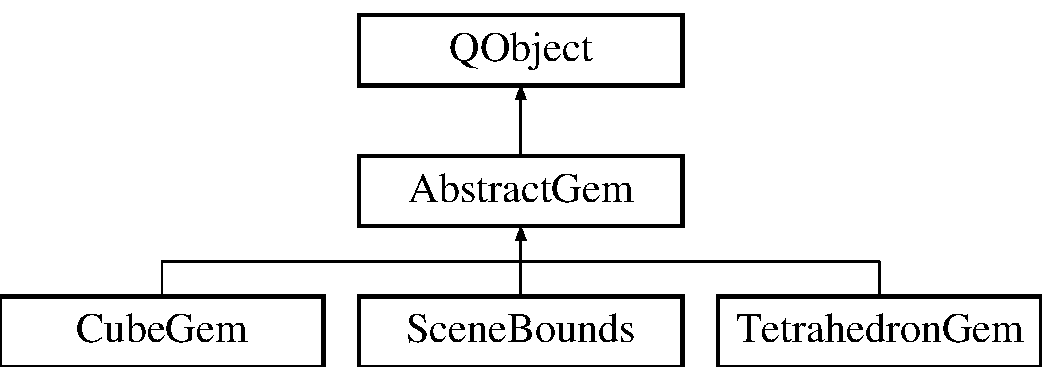
\includegraphics[height=3.000000cm]{class_abstract_gem}
\end{center}
\end{figure}
\subsection*{Public Slots}
\begin{DoxyCompactItemize}
\item 
void \hyperlink{class_abstract_gem_a6198aae1f2f54d73a7a5e66ca60f5f67}{set\+Rotation\+From\+Euler} (const Q\+Vector3\+D \&euler\+Rotation)
\begin{DoxyCompactList}\small\item\em Sets rotation of gem using euler angles. This method is mainly used to set initial rotation. \end{DoxyCompactList}\end{DoxyCompactItemize}
\subsection*{Signals}
\begin{DoxyCompactItemize}
\item 
void \hyperlink{class_abstract_gem_ac84dd4c9b3ea3adf02c1bfa74a29b649}{position\+Changed} ()
\item 
void \hyperlink{class_abstract_gem_a2702e870321deb40a8f056c1fce01094}{rotation\+Changed} ()
\item 
void \hyperlink{class_abstract_gem_a7e6bfe659f09bc68222211a58c365177}{scale\+Changed} ()
\item 
void \hyperlink{class_abstract_gem_ae20ad53d4ddeff9fc13878e7db5a3253}{color\+Changed} ()
\end{DoxyCompactItemize}
\subsection*{Public Member Functions}
\begin{DoxyCompactItemize}
\item 
\hyperlink{class_abstract_gem_a489d032060a42a9a8475309105fc585d}{Abstract\+Gem} (Q\+Object $\ast$parent=0)
\item 
virtual \hyperlink{class_abstract_gem_aafe5a4fa8c354ee562602d7b9ff1656b}{$\sim$\+Abstract\+Gem} ()
\item 
const Q\+Vector3\+D \& \hyperlink{class_abstract_gem_abb92885bcf86f43f069c9a0ef203d770}{color} () const 
\item 
void \hyperlink{class_abstract_gem_ace63416f61034b73969b5a89e3913e6d}{set\+Color} (const Q\+Vector3\+D \&color)
\item 
const \hyperlink{class_gem_data}{Gem\+Data} \& \hyperlink{class_abstract_gem_ac23fb212f3cca79b345f82e19f8c12d5}{data} () const 
\begin{DoxyCompactList}\small\item\em Returns the \hyperlink{class_gem_data}{Gem\+Data} object describing the gem.  This method was not intended to be public, but public access is needed it for rendering. \end{DoxyCompactList}\item 
const Q\+Matrix4x4 \& \hyperlink{class_abstract_gem_a89f90d07bc8a780f053b3c6a5720aeed}{model} () const 
\begin{DoxyCompactList}\small\item\em Constructs normal matrix for gem in order to transform it from objectspace into worldsapce. \end{DoxyCompactList}\item 
const Q\+Vector3\+D \& \hyperlink{class_abstract_gem_a404114854610011363f6d7800985b718}{position} () const 
\item 
virtual void \hyperlink{class_abstract_gem_aaf11fa4b522dc334ebed4f2d031a3e2b}{set\+Position} (const Q\+Vector3\+D \&position)
\item 
qreal \hyperlink{class_abstract_gem_a628481ed4ebff7b282524a003d4392c2}{radius} () const 
\begin{DoxyCompactList}\small\item\em Radius of boundingsphere. This value is influenced by scale and the geometry of gem. \end{DoxyCompactList}\item 
const Q\+Quaternion \& \hyperlink{class_abstract_gem_a4fc9d6ed418b73ec2539e063ebfa70c1}{rotation} () const 
\begin{DoxyCompactList}\small\item\em Rotation around own center. \end{DoxyCompactList}\item 
virtual void \hyperlink{class_abstract_gem_afce4d09f74fec117d27b11a220eee6b9}{set\+Rotation} (const Q\+Quaternion \&rotation)
\begin{DoxyCompactList}\small\item\em Sets the rotation of gem around own center. \end{DoxyCompactList}\item 
void \hyperlink{class_abstract_gem_a5ca6867a835dfe2b49d46dbfb933bfca}{rotate} (const Q\+Quaternion \&quaternion)
\begin{DoxyCompactList}\small\item\em Rotates the gem around the center of the gem. \end{DoxyCompactList}\item 
qreal \hyperlink{class_abstract_gem_aadc1c5925331b573d9aba6c2451c9348}{scale} () const 
\item 
void \hyperlink{class_abstract_gem_a23693f4ebb5260cb21141bbcf3f4ff83}{set\+Scale} (qreal scale\+Factor)
\item 
\hyperlink{abstractgem_8h_a2f0a34b6dac35a9610cab7a1c5fcb444}{Gem\+Type} \hyperlink{class_abstract_gem_a4860dda50d7acab4f507505369da19f8}{type} () const 
\begin{DoxyCompactList}\small\item\em Returns the type of gem, in order to differentiate between types even if you have only Abstract\+Gems. \end{DoxyCompactList}\item 
float \hyperlink{class_abstract_gem_a9f945c4f1b76ae90414ed3229d01dd0b}{bounding\+Sphere\+Intersected\+By} (const \hyperlink{class_light_ray}{Light\+Ray} \&ray, Q\+Vector3\+D $\ast$collision\+Point=nullptr)
\begin{DoxyCompactList}\small\item\em Calculates distance to collision with gem's boundingsphere.  The boundingsphere is specified by gems themself and cannot be influenced from outside. Because the collision point is only calculated with the bondingsphere computation is pretty fast. \end{DoxyCompactList}\item 
virtual float \hyperlink{class_abstract_gem_adc52cc6d78f3494563c50cfd7e0584b4}{intersected\+By} (const \hyperlink{class_light_ray}{Light\+Ray} \&ray, Q\+Vector3\+D $\ast$collision\+Point=nullptr)
\begin{DoxyCompactList}\small\item\em Calcualtes the distance to collision of ray with gem.  This method calculates the real collision point. Therefore, many computations are done especially for complex gems. \end{DoxyCompactList}\item 
virtual \hyperlink{singleton_q_list}{Q\+List}$<$ \hyperlink{class_light_ray}{Light\+Ray} $\ast$ $>$ \hyperlink{class_abstract_gem_ab4f3c6d38acbe59a610c67588e4944d7}{process\+Ray\+Intersection} (const \hyperlink{class_light_ray}{Light\+Ray} \&ray, \hyperlink{class_scene}{Scene} $\ast$scene)
\begin{DoxyCompactList}\small\item\em Calculates all new rays, that will be created by a collision with that gem. Also affect gem attributes. \end{DoxyCompactList}\end{DoxyCompactItemize}
\subsection*{Protected Member Functions}
\begin{DoxyCompactItemize}
\item 
int \hyperlink{class_abstract_gem_a85e872137d38a2c4a9a38f1f0b996bdc}{solve\+Quadric\+Formula} (float a, float b, float c, float \&x1, float \&x2)
\item 
float \hyperlink{class_abstract_gem_a446d8e7a7296203789414ae5b93e0bde}{face\+Intersected\+By} (const \hyperlink{class_light_ray}{Light\+Ray} \&ray, \hyperlink{class_triangle}{Triangle} $\ast$\&intersected\+Face, Q\+Vector3\+D $\ast$collision\+Point=nullptr)
\begin{DoxyCompactList}\small\item\em Finds face of gem intersected by given ray. Ownership of returned face is transferred to caller. \end{DoxyCompactList}\item 
\hyperlink{class_triangle}{Triangle} \hyperlink{class_abstract_gem_a18523ca4a999d5159e38003b3fad5f20}{in\+World\+Coordinates} (const \hyperlink{class_triangle}{Triangle} \&triangle)
\begin{DoxyCompactList}\small\item\em Calculates triangle in world coordinates for given triangle. Therefore, position, rotatition and scale of gem are used. \end{DoxyCompactList}\end{DoxyCompactItemize}
\subsection*{Protected Attributes}
\begin{DoxyCompactItemize}
\item 
\hyperlink{class_gem_data}{Gem\+Data} $\ast$ \hyperlink{class_abstract_gem_a10a337f732ade69f1988659852f837c6}{m\+\_\+data}
\item 
qreal \hyperlink{class_abstract_gem_ab058af121fa66616cab7551e9418048a}{m\+\_\+radius}
\end{DoxyCompactItemize}


\subsection{Detailed Description}
The \hyperlink{class_abstract_gem}{Abstract\+Gem} class is the base class of all gems.  As base class all required information of a gem are stored. Also, useful algorithms for collision detection are provided. Furthermore, this class is supposed to be used within Q\+M\+L. 

\subsection{Constructor \& Destructor Documentation}
\hypertarget{class_abstract_gem_a489d032060a42a9a8475309105fc585d}{\index{Abstract\+Gem@{Abstract\+Gem}!Abstract\+Gem@{Abstract\+Gem}}
\index{Abstract\+Gem@{Abstract\+Gem}!Abstract\+Gem@{Abstract\+Gem}}
\subsubsection[{Abstract\+Gem}]{\setlength{\rightskip}{0pt plus 5cm}Abstract\+Gem\+::\+Abstract\+Gem (
\begin{DoxyParamCaption}
\item[{Q\+Object $\ast$}]{parent = {\ttfamily 0}}
\end{DoxyParamCaption}
)\hspace{0.3cm}{\ttfamily [explicit]}}}\label{class_abstract_gem_a489d032060a42a9a8475309105fc585d}
\hypertarget{class_abstract_gem_aafe5a4fa8c354ee562602d7b9ff1656b}{\index{Abstract\+Gem@{Abstract\+Gem}!````~Abstract\+Gem@{$\sim$\+Abstract\+Gem}}
\index{````~Abstract\+Gem@{$\sim$\+Abstract\+Gem}!Abstract\+Gem@{Abstract\+Gem}}
\subsubsection[{$\sim$\+Abstract\+Gem}]{\setlength{\rightskip}{0pt plus 5cm}Abstract\+Gem\+::$\sim$\+Abstract\+Gem (
\begin{DoxyParamCaption}
{}
\end{DoxyParamCaption}
)\hspace{0.3cm}{\ttfamily [virtual]}}}\label{class_abstract_gem_aafe5a4fa8c354ee562602d7b9ff1656b}


\subsection{Member Function Documentation}
\hypertarget{class_abstract_gem_a9f945c4f1b76ae90414ed3229d01dd0b}{\index{Abstract\+Gem@{Abstract\+Gem}!bounding\+Sphere\+Intersected\+By@{bounding\+Sphere\+Intersected\+By}}
\index{bounding\+Sphere\+Intersected\+By@{bounding\+Sphere\+Intersected\+By}!Abstract\+Gem@{Abstract\+Gem}}
\subsubsection[{bounding\+Sphere\+Intersected\+By}]{\setlength{\rightskip}{0pt plus 5cm}float Abstract\+Gem\+::bounding\+Sphere\+Intersected\+By (
\begin{DoxyParamCaption}
\item[{const {\bf Light\+Ray} \&}]{ray, }
\item[{Q\+Vector3\+D $\ast$}]{collision\+Point = {\ttfamily nullptr}}
\end{DoxyParamCaption}
)}}\label{class_abstract_gem_a9f945c4f1b76ae90414ed3229d01dd0b}


Calculates distance to collision with gem's boundingsphere.  The boundingsphere is specified by gems themself and cannot be influenced from outside. Because the collision point is only calculated with the bondingsphere computation is pretty fast. 


\begin{DoxyParams}{Parameters}
{\em ray} & The ray which might collide with gem's boundingsphere \\
\hline
{\em collision\+Point} & Optional parameter. If provided the collision point of ray with boundingsphere is written into. If no collision occurs the maximum float value is written into all components. \\
\hline
\end{DoxyParams}
\begin{DoxyReturn}{Returns}
The factor you need to apply ray.\+direction() to ray.\+start\+Position(). If no collision occurs maximum float value is returned. Do not compare this value with return values of \hyperlink{class_abstract_gem_adc52cc6d78f3494563c50cfd7e0584b4}{intersected\+By()}  \hyperlink{class_abstract_gem_adc52cc6d78f3494563c50cfd7e0584b4}{intersected\+By()} 
\end{DoxyReturn}
\hypertarget{class_abstract_gem_abb92885bcf86f43f069c9a0ef203d770}{\index{Abstract\+Gem@{Abstract\+Gem}!color@{color}}
\index{color@{color}!Abstract\+Gem@{Abstract\+Gem}}
\subsubsection[{color}]{\setlength{\rightskip}{0pt plus 5cm}const Q\+Vector3\+D\& Abstract\+Gem\+::color (
\begin{DoxyParamCaption}
{}
\end{DoxyParamCaption}
) const}}\label{class_abstract_gem_abb92885bcf86f43f069c9a0ef203d770}
\hypertarget{class_abstract_gem_ae20ad53d4ddeff9fc13878e7db5a3253}{\index{Abstract\+Gem@{Abstract\+Gem}!color\+Changed@{color\+Changed}}
\index{color\+Changed@{color\+Changed}!Abstract\+Gem@{Abstract\+Gem}}
\subsubsection[{color\+Changed}]{\setlength{\rightskip}{0pt plus 5cm}void Abstract\+Gem\+::color\+Changed (
\begin{DoxyParamCaption}
{}
\end{DoxyParamCaption}
)\hspace{0.3cm}{\ttfamily [signal]}}}\label{class_abstract_gem_ae20ad53d4ddeff9fc13878e7db5a3253}
\hypertarget{class_abstract_gem_ac23fb212f3cca79b345f82e19f8c12d5}{\index{Abstract\+Gem@{Abstract\+Gem}!data@{data}}
\index{data@{data}!Abstract\+Gem@{Abstract\+Gem}}
\subsubsection[{data}]{\setlength{\rightskip}{0pt plus 5cm}const {\bf Gem\+Data} \& Abstract\+Gem\+::data (
\begin{DoxyParamCaption}
{}
\end{DoxyParamCaption}
) const}}\label{class_abstract_gem_ac23fb212f3cca79b345f82e19f8c12d5}


Returns the \hyperlink{class_gem_data}{Gem\+Data} object describing the gem.  This method was not intended to be public, but public access is needed it for rendering. 

\begin{DoxyReturn}{Returns}

\end{DoxyReturn}
\hypertarget{class_abstract_gem_a446d8e7a7296203789414ae5b93e0bde}{\index{Abstract\+Gem@{Abstract\+Gem}!face\+Intersected\+By@{face\+Intersected\+By}}
\index{face\+Intersected\+By@{face\+Intersected\+By}!Abstract\+Gem@{Abstract\+Gem}}
\subsubsection[{face\+Intersected\+By}]{\setlength{\rightskip}{0pt plus 5cm}float Abstract\+Gem\+::face\+Intersected\+By (
\begin{DoxyParamCaption}
\item[{const {\bf Light\+Ray} \&}]{ray, }
\item[{{\bf Triangle} $\ast$\&}]{intersected\+Face, }
\item[{Q\+Vector3\+D $\ast$}]{collision\+Point = {\ttfamily nullptr}}
\end{DoxyParamCaption}
)\hspace{0.3cm}{\ttfamily [protected]}}}\label{class_abstract_gem_a446d8e7a7296203789414ae5b93e0bde}


Finds face of gem intersected by given ray. Ownership of returned face is transferred to caller. 


\begin{DoxyParams}{Parameters}
{\em ray} & Ray that might intersect gem \\
\hline
{\em intersected\+Face} & A pointer to intersected face is written into. Because this triangle is in worldspace and for performance reasons the ownership of face is transferred to caller. If ray does not intersect nullptr is written. \\
\hline
{\em collision\+Point} & Optional parameter. If the given pointer is not nullptr the collisionpoint is written into. \\
\hline
\end{DoxyParams}
\begin{DoxyReturn}{Returns}
Returns distance to collisionpoint. If no collission occured the value is maximum of float. 
\end{DoxyReturn}
\hypertarget{class_abstract_gem_adc52cc6d78f3494563c50cfd7e0584b4}{\index{Abstract\+Gem@{Abstract\+Gem}!intersected\+By@{intersected\+By}}
\index{intersected\+By@{intersected\+By}!Abstract\+Gem@{Abstract\+Gem}}
\subsubsection[{intersected\+By}]{\setlength{\rightskip}{0pt plus 5cm}float Abstract\+Gem\+::intersected\+By (
\begin{DoxyParamCaption}
\item[{const {\bf Light\+Ray} \&}]{ray, }
\item[{Q\+Vector3\+D $\ast$}]{collision\+Point = {\ttfamily nullptr}}
\end{DoxyParamCaption}
)\hspace{0.3cm}{\ttfamily [virtual]}}}\label{class_abstract_gem_adc52cc6d78f3494563c50cfd7e0584b4}


Calcualtes the distance to collision of ray with gem.  This method calculates the real collision point. Therefore, many computations are done especially for complex gems. 


\begin{DoxyParams}{Parameters}
{\em ray} & The ray that might collide with gem. \\
\hline
{\em collision\+Point} & Optional parameter. If a collision occurs the collision point will be written into this else all components contain maximum float values. \\
\hline
\end{DoxyParams}
\begin{DoxyReturn}{Returns}
The factor you need to apply ray.\+normalized\+Direction() to ray.\+start\+Direction(). If no collision occurs this value will be highest possible float. Do not compare this value with return value of boundingsphere\+Intersected\+By()  \hyperlink{class_abstract_gem_a9f945c4f1b76ae90414ed3229d01dd0b}{bounding\+Sphere\+Intersected\+By()} 
\end{DoxyReturn}
\hypertarget{class_abstract_gem_a18523ca4a999d5159e38003b3fad5f20}{\index{Abstract\+Gem@{Abstract\+Gem}!in\+World\+Coordinates@{in\+World\+Coordinates}}
\index{in\+World\+Coordinates@{in\+World\+Coordinates}!Abstract\+Gem@{Abstract\+Gem}}
\subsubsection[{in\+World\+Coordinates}]{\setlength{\rightskip}{0pt plus 5cm}{\bf Triangle} Abstract\+Gem\+::in\+World\+Coordinates (
\begin{DoxyParamCaption}
\item[{const {\bf Triangle} \&}]{triangle}
\end{DoxyParamCaption}
)\hspace{0.3cm}{\ttfamily [protected]}}}\label{class_abstract_gem_a18523ca4a999d5159e38003b3fad5f20}


Calculates triangle in world coordinates for given triangle. Therefore, position, rotatition and scale of gem are used. 


\begin{DoxyParams}{Parameters}
{\em triangle} & Objectspace triangle whose corresponding worldspace triangle should be calculated. \\
\hline
\end{DoxyParams}
\begin{DoxyReturn}{Returns}
Returns the \hyperlink{class_triangle}{Triangle} in world coordinates. 
\end{DoxyReturn}
\hypertarget{class_abstract_gem_a89f90d07bc8a780f053b3c6a5720aeed}{\index{Abstract\+Gem@{Abstract\+Gem}!model@{model}}
\index{model@{model}!Abstract\+Gem@{Abstract\+Gem}}
\subsubsection[{model}]{\setlength{\rightskip}{0pt plus 5cm}const Q\+Matrix4x4 \& Abstract\+Gem\+::model (
\begin{DoxyParamCaption}
{}
\end{DoxyParamCaption}
) const}}\label{class_abstract_gem_a89f90d07bc8a780f053b3c6a5720aeed}


Constructs normal matrix for gem in order to transform it from objectspace into worldsapce. 

\begin{DoxyReturn}{Returns}

\end{DoxyReturn}
\hypertarget{class_abstract_gem_a404114854610011363f6d7800985b718}{\index{Abstract\+Gem@{Abstract\+Gem}!position@{position}}
\index{position@{position}!Abstract\+Gem@{Abstract\+Gem}}
\subsubsection[{position}]{\setlength{\rightskip}{0pt plus 5cm}const Q\+Vector3\+D\& Abstract\+Gem\+::position (
\begin{DoxyParamCaption}
{}
\end{DoxyParamCaption}
) const}}\label{class_abstract_gem_a404114854610011363f6d7800985b718}
\hypertarget{class_abstract_gem_ac84dd4c9b3ea3adf02c1bfa74a29b649}{\index{Abstract\+Gem@{Abstract\+Gem}!position\+Changed@{position\+Changed}}
\index{position\+Changed@{position\+Changed}!Abstract\+Gem@{Abstract\+Gem}}
\subsubsection[{position\+Changed}]{\setlength{\rightskip}{0pt plus 5cm}void Abstract\+Gem\+::position\+Changed (
\begin{DoxyParamCaption}
{}
\end{DoxyParamCaption}
)\hspace{0.3cm}{\ttfamily [signal]}}}\label{class_abstract_gem_ac84dd4c9b3ea3adf02c1bfa74a29b649}
\hypertarget{class_abstract_gem_ab4f3c6d38acbe59a610c67588e4944d7}{\index{Abstract\+Gem@{Abstract\+Gem}!process\+Ray\+Intersection@{process\+Ray\+Intersection}}
\index{process\+Ray\+Intersection@{process\+Ray\+Intersection}!Abstract\+Gem@{Abstract\+Gem}}
\subsubsection[{process\+Ray\+Intersection}]{\setlength{\rightskip}{0pt plus 5cm}{\bf Q\+List}$<$ {\bf Light\+Ray} $\ast$ $>$ Abstract\+Gem\+::process\+Ray\+Intersection (
\begin{DoxyParamCaption}
\item[{const {\bf Light\+Ray} \&}]{ray, }
\item[{{\bf Scene} $\ast$}]{scene}
\end{DoxyParamCaption}
)\hspace{0.3cm}{\ttfamily [virtual]}}}\label{class_abstract_gem_ab4f3c6d38acbe59a610c67588e4944d7}


Calculates all new rays, that will be created by a collision with that gem. Also affect gem attributes. 


\begin{DoxyParams}{Parameters}
{\em ray} & Ray that might collide. \\
\hline
{\em scene} & The scene the ray and gem are in. This is needed in order to calculate new rays appropriately. \\
\hline
\end{DoxyParams}
\begin{DoxyReturn}{Returns}
A List of light rays that should be added to scene. If no collision occurs, the list is empty. Ownership of rays contained in list is transferred to caller. 
\end{DoxyReturn}


Reimplemented in \hyperlink{class_scene_bounds_aeac6aafe6081e8efd6b4180e86346dc0}{Scene\+Bounds}.

\hypertarget{class_abstract_gem_a628481ed4ebff7b282524a003d4392c2}{\index{Abstract\+Gem@{Abstract\+Gem}!radius@{radius}}
\index{radius@{radius}!Abstract\+Gem@{Abstract\+Gem}}
\subsubsection[{radius}]{\setlength{\rightskip}{0pt plus 5cm}qreal Abstract\+Gem\+::radius (
\begin{DoxyParamCaption}
{}
\end{DoxyParamCaption}
) const}}\label{class_abstract_gem_a628481ed4ebff7b282524a003d4392c2}


Radius of boundingsphere. This value is influenced by scale and the geometry of gem. 

\begin{DoxyReturn}{Returns}

\end{DoxyReturn}
\hypertarget{class_abstract_gem_a5ca6867a835dfe2b49d46dbfb933bfca}{\index{Abstract\+Gem@{Abstract\+Gem}!rotate@{rotate}}
\index{rotate@{rotate}!Abstract\+Gem@{Abstract\+Gem}}
\subsubsection[{rotate}]{\setlength{\rightskip}{0pt plus 5cm}void Abstract\+Gem\+::rotate (
\begin{DoxyParamCaption}
\item[{const Q\+Quaternion \&}]{quaternion}
\end{DoxyParamCaption}
)}}\label{class_abstract_gem_a5ca6867a835dfe2b49d46dbfb933bfca}


Rotates the gem around the center of the gem. 


\begin{DoxyParams}{Parameters}
{\em quaternion} & Specifies how the gem should be rotated. \\
\hline
\end{DoxyParams}
\hypertarget{class_abstract_gem_a4fc9d6ed418b73ec2539e063ebfa70c1}{\index{Abstract\+Gem@{Abstract\+Gem}!rotation@{rotation}}
\index{rotation@{rotation}!Abstract\+Gem@{Abstract\+Gem}}
\subsubsection[{rotation}]{\setlength{\rightskip}{0pt plus 5cm}const Q\+Quaternion\& Abstract\+Gem\+::rotation (
\begin{DoxyParamCaption}
{}
\end{DoxyParamCaption}
) const}}\label{class_abstract_gem_a4fc9d6ed418b73ec2539e063ebfa70c1}


Rotation around own center. 

\begin{DoxyReturn}{Returns}

\end{DoxyReturn}
\hypertarget{class_abstract_gem_a2702e870321deb40a8f056c1fce01094}{\index{Abstract\+Gem@{Abstract\+Gem}!rotation\+Changed@{rotation\+Changed}}
\index{rotation\+Changed@{rotation\+Changed}!Abstract\+Gem@{Abstract\+Gem}}
\subsubsection[{rotation\+Changed}]{\setlength{\rightskip}{0pt plus 5cm}void Abstract\+Gem\+::rotation\+Changed (
\begin{DoxyParamCaption}
{}
\end{DoxyParamCaption}
)\hspace{0.3cm}{\ttfamily [signal]}}}\label{class_abstract_gem_a2702e870321deb40a8f056c1fce01094}
\hypertarget{class_abstract_gem_aadc1c5925331b573d9aba6c2451c9348}{\index{Abstract\+Gem@{Abstract\+Gem}!scale@{scale}}
\index{scale@{scale}!Abstract\+Gem@{Abstract\+Gem}}
\subsubsection[{scale}]{\setlength{\rightskip}{0pt plus 5cm}qreal Abstract\+Gem\+::scale (
\begin{DoxyParamCaption}
{}
\end{DoxyParamCaption}
) const}}\label{class_abstract_gem_aadc1c5925331b573d9aba6c2451c9348}
\hypertarget{class_abstract_gem_a7e6bfe659f09bc68222211a58c365177}{\index{Abstract\+Gem@{Abstract\+Gem}!scale\+Changed@{scale\+Changed}}
\index{scale\+Changed@{scale\+Changed}!Abstract\+Gem@{Abstract\+Gem}}
\subsubsection[{scale\+Changed}]{\setlength{\rightskip}{0pt plus 5cm}void Abstract\+Gem\+::scale\+Changed (
\begin{DoxyParamCaption}
{}
\end{DoxyParamCaption}
)\hspace{0.3cm}{\ttfamily [signal]}}}\label{class_abstract_gem_a7e6bfe659f09bc68222211a58c365177}
\hypertarget{class_abstract_gem_ace63416f61034b73969b5a89e3913e6d}{\index{Abstract\+Gem@{Abstract\+Gem}!set\+Color@{set\+Color}}
\index{set\+Color@{set\+Color}!Abstract\+Gem@{Abstract\+Gem}}
\subsubsection[{set\+Color}]{\setlength{\rightskip}{0pt plus 5cm}void Abstract\+Gem\+::set\+Color (
\begin{DoxyParamCaption}
\item[{const Q\+Vector3\+D \&}]{color}
\end{DoxyParamCaption}
)}}\label{class_abstract_gem_ace63416f61034b73969b5a89e3913e6d}
\hypertarget{class_abstract_gem_aaf11fa4b522dc334ebed4f2d031a3e2b}{\index{Abstract\+Gem@{Abstract\+Gem}!set\+Position@{set\+Position}}
\index{set\+Position@{set\+Position}!Abstract\+Gem@{Abstract\+Gem}}
\subsubsection[{set\+Position}]{\setlength{\rightskip}{0pt plus 5cm}void Abstract\+Gem\+::set\+Position (
\begin{DoxyParamCaption}
\item[{const Q\+Vector3\+D \&}]{position}
\end{DoxyParamCaption}
)\hspace{0.3cm}{\ttfamily [virtual]}}}\label{class_abstract_gem_aaf11fa4b522dc334ebed4f2d031a3e2b}


Reimplemented in \hyperlink{class_scene_bounds_a26db5e7928d3ac7d0257dc52e1ed4e77}{Scene\+Bounds}.

\hypertarget{class_abstract_gem_afce4d09f74fec117d27b11a220eee6b9}{\index{Abstract\+Gem@{Abstract\+Gem}!set\+Rotation@{set\+Rotation}}
\index{set\+Rotation@{set\+Rotation}!Abstract\+Gem@{Abstract\+Gem}}
\subsubsection[{set\+Rotation}]{\setlength{\rightskip}{0pt plus 5cm}void Abstract\+Gem\+::set\+Rotation (
\begin{DoxyParamCaption}
\item[{const Q\+Quaternion \&}]{rotation}
\end{DoxyParamCaption}
)\hspace{0.3cm}{\ttfamily [virtual]}}}\label{class_abstract_gem_afce4d09f74fec117d27b11a220eee6b9}


Sets the rotation of gem around own center. 


\begin{DoxyParams}{Parameters}
{\em rotation} & Value the roation will be set to.  \hyperlink{class_abstract_gem_a6198aae1f2f54d73a7a5e66ca60f5f67}{set\+Rotation\+From\+Euler()} \\
\hline
\end{DoxyParams}


Reimplemented in \hyperlink{class_scene_bounds_a2e7b2f2e66700b414584ca6b407faf72}{Scene\+Bounds}.

\hypertarget{class_abstract_gem_a6198aae1f2f54d73a7a5e66ca60f5f67}{\index{Abstract\+Gem@{Abstract\+Gem}!set\+Rotation\+From\+Euler@{set\+Rotation\+From\+Euler}}
\index{set\+Rotation\+From\+Euler@{set\+Rotation\+From\+Euler}!Abstract\+Gem@{Abstract\+Gem}}
\subsubsection[{set\+Rotation\+From\+Euler}]{\setlength{\rightskip}{0pt plus 5cm}void Abstract\+Gem\+::set\+Rotation\+From\+Euler (
\begin{DoxyParamCaption}
\item[{const Q\+Vector3\+D \&}]{euler\+Rotation}
\end{DoxyParamCaption}
)\hspace{0.3cm}{\ttfamily [slot]}}}\label{class_abstract_gem_a6198aae1f2f54d73a7a5e66ca60f5f67}


Sets rotation of gem using euler angles. This method is mainly used to set initial rotation. 


\begin{DoxyParams}{Parameters}
{\em euler\+Rotation} & Q\+Vector3\+D containing the euler angles. The member of euler\+Vector contains corresponding rotation along axis (x component = rotation around x axis). The angle around axis is specified in degrees. \\
\hline
\end{DoxyParams}
\hypertarget{class_abstract_gem_a23693f4ebb5260cb21141bbcf3f4ff83}{\index{Abstract\+Gem@{Abstract\+Gem}!set\+Scale@{set\+Scale}}
\index{set\+Scale@{set\+Scale}!Abstract\+Gem@{Abstract\+Gem}}
\subsubsection[{set\+Scale}]{\setlength{\rightskip}{0pt plus 5cm}void Abstract\+Gem\+::set\+Scale (
\begin{DoxyParamCaption}
\item[{qreal}]{scale\+Factor}
\end{DoxyParamCaption}
)}}\label{class_abstract_gem_a23693f4ebb5260cb21141bbcf3f4ff83}
\hypertarget{class_abstract_gem_a85e872137d38a2c4a9a38f1f0b996bdc}{\index{Abstract\+Gem@{Abstract\+Gem}!solve\+Quadric\+Formula@{solve\+Quadric\+Formula}}
\index{solve\+Quadric\+Formula@{solve\+Quadric\+Formula}!Abstract\+Gem@{Abstract\+Gem}}
\subsubsection[{solve\+Quadric\+Formula}]{\setlength{\rightskip}{0pt plus 5cm}int Abstract\+Gem\+::solve\+Quadric\+Formula (
\begin{DoxyParamCaption}
\item[{float}]{a, }
\item[{float}]{b, }
\item[{float}]{c, }
\item[{float \&}]{x1, }
\item[{float \&}]{x2}
\end{DoxyParamCaption}
)\hspace{0.3cm}{\ttfamily [protected]}}}\label{class_abstract_gem_a85e872137d38a2c4a9a38f1f0b996bdc}
\hypertarget{class_abstract_gem_a4860dda50d7acab4f507505369da19f8}{\index{Abstract\+Gem@{Abstract\+Gem}!type@{type}}
\index{type@{type}!Abstract\+Gem@{Abstract\+Gem}}
\subsubsection[{type}]{\setlength{\rightskip}{0pt plus 5cm}{\bf Gem\+Type} Abstract\+Gem\+::type (
\begin{DoxyParamCaption}
{}
\end{DoxyParamCaption}
) const}}\label{class_abstract_gem_a4860dda50d7acab4f507505369da19f8}


Returns the type of gem, in order to differentiate between types even if you have only Abstract\+Gems. 

\begin{DoxyReturn}{Returns}

\end{DoxyReturn}


\subsection{Member Data Documentation}
\hypertarget{class_abstract_gem_a10a337f732ade69f1988659852f837c6}{\index{Abstract\+Gem@{Abstract\+Gem}!m\+\_\+data@{m\+\_\+data}}
\index{m\+\_\+data@{m\+\_\+data}!Abstract\+Gem@{Abstract\+Gem}}
\subsubsection[{m\+\_\+data}]{\setlength{\rightskip}{0pt plus 5cm}{\bf Gem\+Data}$\ast$ Abstract\+Gem\+::m\+\_\+data\hspace{0.3cm}{\ttfamily [protected]}}}\label{class_abstract_gem_a10a337f732ade69f1988659852f837c6}
\hypertarget{class_abstract_gem_ab058af121fa66616cab7551e9418048a}{\index{Abstract\+Gem@{Abstract\+Gem}!m\+\_\+radius@{m\+\_\+radius}}
\index{m\+\_\+radius@{m\+\_\+radius}!Abstract\+Gem@{Abstract\+Gem}}
\subsubsection[{m\+\_\+radius}]{\setlength{\rightskip}{0pt plus 5cm}qreal Abstract\+Gem\+::m\+\_\+radius\hspace{0.3cm}{\ttfamily [protected]}}}\label{class_abstract_gem_ab058af121fa66616cab7551e9418048a}


The documentation for this class was generated from the following files\+:\begin{DoxyCompactItemize}
\item 
\hyperlink{abstractgem_8h}{abstractgem.\+h}\item 
\hyperlink{abstractgem_8cpp}{abstractgem.\+cpp}\end{DoxyCompactItemize}

\hypertarget{class_blur_effect}{\section{Blur\+Effect Class Reference}
\label{class_blur_effect}\index{Blur\+Effect@{Blur\+Effect}}
}


The \hyperlink{class_blur_effect}{Blur\+Effect} blurs a given texture.  




{\ttfamily \#include $<$blureffect.\+h$>$}

Inheritance diagram for Blur\+Effect\+:\begin{figure}[H]
\begin{center}
\leavevmode
\includegraphics[height=2.000000cm]{class_blur_effect}
\end{center}
\end{figure}
\subsection*{Public Member Functions}
\begin{DoxyCompactItemize}
\item 
\hyperlink{class_blur_effect_a3653fdf73228f64b5fab03589060c704}{Blur\+Effect} (Q\+Open\+G\+L\+Functions \&gl, uint glow\+Texture, Q\+Object $\ast$parent=nullptr)
\begin{DoxyCompactList}\small\item\em Creates a new \hyperlink{class_blur_effect}{Blur\+Effect} that will blur a specified texture everytime \hyperlink{class_blur_effect_a0317d7ce7078d1e28e7e5b37fb60b9f3}{blur()} is called. \end{DoxyCompactList}\item 
virtual \hyperlink{class_blur_effect_aeb30b45dd769774ff0f0706a4ad6566c}{$\sim$\+Blur\+Effect} ()
\item 
void \hyperlink{class_blur_effect_a0317d7ce7078d1e28e7e5b37fb60b9f3}{blur} (const Q\+Size \&texture\+Size)
\begin{DoxyCompactList}\small\item\em Blurs previous set texture.  The texture is blurred using two seperated passes of gauss blur. The result is a gaussblur with 9x9 kernel. \end{DoxyCompactList}\end{DoxyCompactItemize}
\subsection*{Protected Member Functions}
\begin{DoxyCompactItemize}
\item 
void \hyperlink{class_blur_effect_a735fa8b4020353e440d226e3a48a9e46}{initialize} ()
\item 
void \hyperlink{class_blur_effect_a673b5ec9a6f4a32bc0bab462b32c7200}{initialize\+F\+B\+Os} ()
\item 
void \hyperlink{class_blur_effect_a3acf8584853e2a2befdbb69eeb65aa2a}{initialize\+Shader\+Programs} ()
\item 
void \hyperlink{class_blur_effect_ad25107035e2585492d3501d8d2d51aa2}{render\+Gauss\+Horizontal} (const Q\+Size \&texture\+Size)
\begin{DoxyCompactList}\small\item\em Blurs texture horizontally. \end{DoxyCompactList}\item 
void \hyperlink{class_blur_effect_aaaaec0e2eb4530834e7ab3ad8beec231}{render\+Gauss\+Vertical} (const Q\+Size \&texture\+Size)
\begin{DoxyCompactList}\small\item\em Blurs texture vertically. \end{DoxyCompactList}\end{DoxyCompactItemize}
\subsection*{Protected Attributes}
\begin{DoxyCompactItemize}
\item 
Q\+Open\+G\+L\+Functions \& \hyperlink{class_blur_effect_a60e476bb206ce650162006e19891f4e2}{m\+\_\+gl}
\item 
Q\+Map$<$ \hyperlink{shaderprograms_8h_ada89718f8d394b2cc093eb9770c554ff}{Shader\+Programs}, \\*
Q\+Open\+G\+L\+Shader\+Program $\ast$ $>$ $\ast$ \hyperlink{class_blur_effect_a36f1750676d9a4b935609300a2c8853c}{m\+\_\+shader\+Programs}
\item 
bool \hyperlink{class_blur_effect_abd260e17d64d3e819c9817e2ae92a33d}{m\+\_\+initialized}
\item 
uint \hyperlink{class_blur_effect_a3cf63e0dc804b038a9348923a5df12f5}{m\+\_\+blur\+F\+B\+O}
\item 
uint \hyperlink{class_blur_effect_a8d3832820bc3cf08171d449cc0dc9430}{m\+\_\+blur\+Texture}
\item 
uint \hyperlink{class_blur_effect_a8bcdeba40d4a73e06a02dc7507ed498e}{m\+\_\+secondary\+Blur\+F\+B\+O}
\item 
uint \hyperlink{class_blur_effect_a1e068c508f32617c867a92a56d521888}{m\+\_\+secondary\+Blur\+Texture}
\item 
Q\+Size $\ast$ \hyperlink{class_blur_effect_a8513aa58d2ff05cc6b135f60c25d0710}{m\+\_\+used\+Viewport}
\item 
\hyperlink{class_screen_aligned_quad}{Screen\+Aligned\+Quad} $\ast$ \hyperlink{class_blur_effect_aa5fb6e7e38f9548b89f7cc6e8de0882a}{m\+\_\+quad}
\end{DoxyCompactItemize}


\subsection{Detailed Description}
The \hyperlink{class_blur_effect}{Blur\+Effect} blurs a given texture. 

\subsection{Constructor \& Destructor Documentation}
\hypertarget{class_blur_effect_a3653fdf73228f64b5fab03589060c704}{\index{Blur\+Effect@{Blur\+Effect}!Blur\+Effect@{Blur\+Effect}}
\index{Blur\+Effect@{Blur\+Effect}!Blur\+Effect@{Blur\+Effect}}
\subsubsection[{Blur\+Effect}]{\setlength{\rightskip}{0pt plus 5cm}Blur\+Effect\+::\+Blur\+Effect (
\begin{DoxyParamCaption}
\item[{Q\+Open\+G\+L\+Functions \&}]{gl, }
\item[{uint}]{glow\+Texture, }
\item[{Q\+Object $\ast$}]{parent = {\ttfamily nullptr}}
\end{DoxyParamCaption}
)}}\label{class_blur_effect_a3653fdf73228f64b5fab03589060c704}


Creates a new \hyperlink{class_blur_effect}{Blur\+Effect} that will blur a specified texture everytime \hyperlink{class_blur_effect_a0317d7ce7078d1e28e7e5b37fb60b9f3}{blur()} is called. 


\begin{DoxyParams}{Parameters}
{\em gl} & The Q\+Open\+G\+L\+Funtions will be used for all gl-\/calls. \\
\hline
{\em glow\+Texture} & The texture that will be blurred. \\
\hline
{\em parent} & Q\+Object-\/parent \\
\hline
\end{DoxyParams}
\hypertarget{class_blur_effect_aeb30b45dd769774ff0f0706a4ad6566c}{\index{Blur\+Effect@{Blur\+Effect}!````~Blur\+Effect@{$\sim$\+Blur\+Effect}}
\index{````~Blur\+Effect@{$\sim$\+Blur\+Effect}!Blur\+Effect@{Blur\+Effect}}
\subsubsection[{$\sim$\+Blur\+Effect}]{\setlength{\rightskip}{0pt plus 5cm}Blur\+Effect\+::$\sim$\+Blur\+Effect (
\begin{DoxyParamCaption}
{}
\end{DoxyParamCaption}
)\hspace{0.3cm}{\ttfamily [virtual]}}}\label{class_blur_effect_aeb30b45dd769774ff0f0706a4ad6566c}


\subsection{Member Function Documentation}
\hypertarget{class_blur_effect_a0317d7ce7078d1e28e7e5b37fb60b9f3}{\index{Blur\+Effect@{Blur\+Effect}!blur@{blur}}
\index{blur@{blur}!Blur\+Effect@{Blur\+Effect}}
\subsubsection[{blur}]{\setlength{\rightskip}{0pt plus 5cm}void Blur\+Effect\+::blur (
\begin{DoxyParamCaption}
\item[{const Q\+Size \&}]{texture\+Size}
\end{DoxyParamCaption}
)}}\label{class_blur_effect_a0317d7ce7078d1e28e7e5b37fb60b9f3}


Blurs previous set texture.  The texture is blurred using two seperated passes of gauss blur. The result is a gaussblur with 9x9 kernel. 


\begin{DoxyParams}{Parameters}
{\em texture\+Size} & The size of texture, because changing texture sizes is supported. \\
\hline
\end{DoxyParams}
\hypertarget{class_blur_effect_a735fa8b4020353e440d226e3a48a9e46}{\index{Blur\+Effect@{Blur\+Effect}!initialize@{initialize}}
\index{initialize@{initialize}!Blur\+Effect@{Blur\+Effect}}
\subsubsection[{initialize}]{\setlength{\rightskip}{0pt plus 5cm}void Blur\+Effect\+::initialize (
\begin{DoxyParamCaption}
{}
\end{DoxyParamCaption}
)\hspace{0.3cm}{\ttfamily [protected]}}}\label{class_blur_effect_a735fa8b4020353e440d226e3a48a9e46}
\hypertarget{class_blur_effect_a673b5ec9a6f4a32bc0bab462b32c7200}{\index{Blur\+Effect@{Blur\+Effect}!initialize\+F\+B\+Os@{initialize\+F\+B\+Os}}
\index{initialize\+F\+B\+Os@{initialize\+F\+B\+Os}!Blur\+Effect@{Blur\+Effect}}
\subsubsection[{initialize\+F\+B\+Os}]{\setlength{\rightskip}{0pt plus 5cm}void Blur\+Effect\+::initialize\+F\+B\+Os (
\begin{DoxyParamCaption}
{}
\end{DoxyParamCaption}
)\hspace{0.3cm}{\ttfamily [protected]}}}\label{class_blur_effect_a673b5ec9a6f4a32bc0bab462b32c7200}
\hypertarget{class_blur_effect_a3acf8584853e2a2befdbb69eeb65aa2a}{\index{Blur\+Effect@{Blur\+Effect}!initialize\+Shader\+Programs@{initialize\+Shader\+Programs}}
\index{initialize\+Shader\+Programs@{initialize\+Shader\+Programs}!Blur\+Effect@{Blur\+Effect}}
\subsubsection[{initialize\+Shader\+Programs}]{\setlength{\rightskip}{0pt plus 5cm}void Blur\+Effect\+::initialize\+Shader\+Programs (
\begin{DoxyParamCaption}
{}
\end{DoxyParamCaption}
)\hspace{0.3cm}{\ttfamily [protected]}}}\label{class_blur_effect_a3acf8584853e2a2befdbb69eeb65aa2a}
\hypertarget{class_blur_effect_ad25107035e2585492d3501d8d2d51aa2}{\index{Blur\+Effect@{Blur\+Effect}!render\+Gauss\+Horizontal@{render\+Gauss\+Horizontal}}
\index{render\+Gauss\+Horizontal@{render\+Gauss\+Horizontal}!Blur\+Effect@{Blur\+Effect}}
\subsubsection[{render\+Gauss\+Horizontal}]{\setlength{\rightskip}{0pt plus 5cm}void Blur\+Effect\+::render\+Gauss\+Horizontal (
\begin{DoxyParamCaption}
\item[{const Q\+Size \&}]{texture\+Size}
\end{DoxyParamCaption}
)\hspace{0.3cm}{\ttfamily [protected]}}}\label{class_blur_effect_ad25107035e2585492d3501d8d2d51aa2}


Blurs texture horizontally. 


\begin{DoxyParams}{Parameters}
{\em texture\+Size} & The current size of texture that is blurred. \\
\hline
\end{DoxyParams}
\hypertarget{class_blur_effect_aaaaec0e2eb4530834e7ab3ad8beec231}{\index{Blur\+Effect@{Blur\+Effect}!render\+Gauss\+Vertical@{render\+Gauss\+Vertical}}
\index{render\+Gauss\+Vertical@{render\+Gauss\+Vertical}!Blur\+Effect@{Blur\+Effect}}
\subsubsection[{render\+Gauss\+Vertical}]{\setlength{\rightskip}{0pt plus 5cm}void Blur\+Effect\+::render\+Gauss\+Vertical (
\begin{DoxyParamCaption}
\item[{const Q\+Size \&}]{texture\+Size}
\end{DoxyParamCaption}
)\hspace{0.3cm}{\ttfamily [protected]}}}\label{class_blur_effect_aaaaec0e2eb4530834e7ab3ad8beec231}


Blurs texture vertically. 


\begin{DoxyParams}{Parameters}
{\em texture\+Size} & The current size of texture that is blurred. \\
\hline
\end{DoxyParams}


\subsection{Member Data Documentation}
\hypertarget{class_blur_effect_a3cf63e0dc804b038a9348923a5df12f5}{\index{Blur\+Effect@{Blur\+Effect}!m\+\_\+blur\+F\+B\+O@{m\+\_\+blur\+F\+B\+O}}
\index{m\+\_\+blur\+F\+B\+O@{m\+\_\+blur\+F\+B\+O}!Blur\+Effect@{Blur\+Effect}}
\subsubsection[{m\+\_\+blur\+F\+B\+O}]{\setlength{\rightskip}{0pt plus 5cm}uint Blur\+Effect\+::m\+\_\+blur\+F\+B\+O\hspace{0.3cm}{\ttfamily [protected]}}}\label{class_blur_effect_a3cf63e0dc804b038a9348923a5df12f5}
\hypertarget{class_blur_effect_a8d3832820bc3cf08171d449cc0dc9430}{\index{Blur\+Effect@{Blur\+Effect}!m\+\_\+blur\+Texture@{m\+\_\+blur\+Texture}}
\index{m\+\_\+blur\+Texture@{m\+\_\+blur\+Texture}!Blur\+Effect@{Blur\+Effect}}
\subsubsection[{m\+\_\+blur\+Texture}]{\setlength{\rightskip}{0pt plus 5cm}uint Blur\+Effect\+::m\+\_\+blur\+Texture\hspace{0.3cm}{\ttfamily [protected]}}}\label{class_blur_effect_a8d3832820bc3cf08171d449cc0dc9430}
\hypertarget{class_blur_effect_a60e476bb206ce650162006e19891f4e2}{\index{Blur\+Effect@{Blur\+Effect}!m\+\_\+gl@{m\+\_\+gl}}
\index{m\+\_\+gl@{m\+\_\+gl}!Blur\+Effect@{Blur\+Effect}}
\subsubsection[{m\+\_\+gl}]{\setlength{\rightskip}{0pt plus 5cm}Q\+Open\+G\+L\+Functions\& Blur\+Effect\+::m\+\_\+gl\hspace{0.3cm}{\ttfamily [protected]}}}\label{class_blur_effect_a60e476bb206ce650162006e19891f4e2}
\hypertarget{class_blur_effect_abd260e17d64d3e819c9817e2ae92a33d}{\index{Blur\+Effect@{Blur\+Effect}!m\+\_\+initialized@{m\+\_\+initialized}}
\index{m\+\_\+initialized@{m\+\_\+initialized}!Blur\+Effect@{Blur\+Effect}}
\subsubsection[{m\+\_\+initialized}]{\setlength{\rightskip}{0pt plus 5cm}bool Blur\+Effect\+::m\+\_\+initialized\hspace{0.3cm}{\ttfamily [protected]}}}\label{class_blur_effect_abd260e17d64d3e819c9817e2ae92a33d}
\hypertarget{class_blur_effect_aa5fb6e7e38f9548b89f7cc6e8de0882a}{\index{Blur\+Effect@{Blur\+Effect}!m\+\_\+quad@{m\+\_\+quad}}
\index{m\+\_\+quad@{m\+\_\+quad}!Blur\+Effect@{Blur\+Effect}}
\subsubsection[{m\+\_\+quad}]{\setlength{\rightskip}{0pt plus 5cm}{\bf Screen\+Aligned\+Quad}$\ast$ Blur\+Effect\+::m\+\_\+quad\hspace{0.3cm}{\ttfamily [protected]}}}\label{class_blur_effect_aa5fb6e7e38f9548b89f7cc6e8de0882a}
\hypertarget{class_blur_effect_a8bcdeba40d4a73e06a02dc7507ed498e}{\index{Blur\+Effect@{Blur\+Effect}!m\+\_\+secondary\+Blur\+F\+B\+O@{m\+\_\+secondary\+Blur\+F\+B\+O}}
\index{m\+\_\+secondary\+Blur\+F\+B\+O@{m\+\_\+secondary\+Blur\+F\+B\+O}!Blur\+Effect@{Blur\+Effect}}
\subsubsection[{m\+\_\+secondary\+Blur\+F\+B\+O}]{\setlength{\rightskip}{0pt plus 5cm}uint Blur\+Effect\+::m\+\_\+secondary\+Blur\+F\+B\+O\hspace{0.3cm}{\ttfamily [protected]}}}\label{class_blur_effect_a8bcdeba40d4a73e06a02dc7507ed498e}
\hypertarget{class_blur_effect_a1e068c508f32617c867a92a56d521888}{\index{Blur\+Effect@{Blur\+Effect}!m\+\_\+secondary\+Blur\+Texture@{m\+\_\+secondary\+Blur\+Texture}}
\index{m\+\_\+secondary\+Blur\+Texture@{m\+\_\+secondary\+Blur\+Texture}!Blur\+Effect@{Blur\+Effect}}
\subsubsection[{m\+\_\+secondary\+Blur\+Texture}]{\setlength{\rightskip}{0pt plus 5cm}uint Blur\+Effect\+::m\+\_\+secondary\+Blur\+Texture\hspace{0.3cm}{\ttfamily [protected]}}}\label{class_blur_effect_a1e068c508f32617c867a92a56d521888}
\hypertarget{class_blur_effect_a36f1750676d9a4b935609300a2c8853c}{\index{Blur\+Effect@{Blur\+Effect}!m\+\_\+shader\+Programs@{m\+\_\+shader\+Programs}}
\index{m\+\_\+shader\+Programs@{m\+\_\+shader\+Programs}!Blur\+Effect@{Blur\+Effect}}
\subsubsection[{m\+\_\+shader\+Programs}]{\setlength{\rightskip}{0pt plus 5cm}Q\+Map$<${\bf Shader\+Programs}, Q\+Open\+G\+L\+Shader\+Program$\ast$$>$$\ast$ Blur\+Effect\+::m\+\_\+shader\+Programs\hspace{0.3cm}{\ttfamily [protected]}}}\label{class_blur_effect_a36f1750676d9a4b935609300a2c8853c}
\hypertarget{class_blur_effect_a8513aa58d2ff05cc6b135f60c25d0710}{\index{Blur\+Effect@{Blur\+Effect}!m\+\_\+used\+Viewport@{m\+\_\+used\+Viewport}}
\index{m\+\_\+used\+Viewport@{m\+\_\+used\+Viewport}!Blur\+Effect@{Blur\+Effect}}
\subsubsection[{m\+\_\+used\+Viewport}]{\setlength{\rightskip}{0pt plus 5cm}Q\+Size$\ast$ Blur\+Effect\+::m\+\_\+used\+Viewport\hspace{0.3cm}{\ttfamily [protected]}}}\label{class_blur_effect_a8513aa58d2ff05cc6b135f60c25d0710}


The documentation for this class was generated from the following files\+:\begin{DoxyCompactItemize}
\item 
\hyperlink{blureffect_8h}{blureffect.\+h}\item 
\hyperlink{blureffect_8cpp}{blureffect.\+cpp}\end{DoxyCompactItemize}

\hypertarget{class_camera}{\section{Camera Class Reference}
\label{class_camera}\index{Camera@{Camera}}
}


The \hyperlink{class_camera}{Camera} class provides view and perspective projection matrices. Additional the viewport of camera is stored.  The view of camera has to be specified by eye, center and up or by position, viewdirection and up. It is allowed to mix both definitions, but it might lead to unexpected behaviour. The perspective projection is specified by field of view, viewport, and near and far plane.  




{\ttfamily \#include $<$camera.\+h$>$}

Inheritance diagram for Camera\+:\begin{figure}[H]
\begin{center}
\leavevmode
\includegraphics[height=2.000000cm]{class_camera}
\end{center}
\end{figure}
\subsection*{Public Slots}
\begin{DoxyCompactItemize}
\item 
void \hyperlink{class_camera_a3ac4fcd89c146068205a3c8b73a86520}{set\+Position} (const Q\+Vector3\+D \&position)
\begin{DoxyCompactList}\small\item\em Sets position of camera to given value. center() will be changed in order to keep view\+Direction() the same. \end{DoxyCompactList}\item 
void \hyperlink{class_camera_a61a059ce3aedc779f9087dda9b5e227c}{set\+View\+Direction} (const Q\+Vector3\+D \&view\+Direction)
\begin{DoxyCompactList}\small\item\em Sets view\+Direction of camera to given vector. center() will be changed in order to keep eye() consistent. \end{DoxyCompactList}\item 
void \hyperlink{class_camera_aa445664f0bf5f3cd892a99125e4bc786}{set\+Eye} (const Q\+Vector3\+D \&eye)
\begin{DoxyCompactList}\small\item\em Sets eye (position) of camera to given value. center() will not be changed, so view\+Direction() is set to center() -\/ eye() \end{DoxyCompactList}\item 
void \hyperlink{class_camera_ae0594124b7a1baf13ef38de7a6bd0ed8}{set\+Center} (const Q\+Vector3\+D \&center)
\begin{DoxyCompactList}\small\item\em Sets center of camera to given value. view\+Direction() will be set to new center() -\/ eye(). \end{DoxyCompactList}\item 
void \hyperlink{class_camera_a037ef3f032c7fc09fa1f044260dd3a09}{set\+Up} (const Q\+Vector3\+D \&up)
\begin{DoxyCompactList}\small\item\em Sets up-\/vector of camera. \end{DoxyCompactList}\item 
void \hyperlink{class_camera_a995075e3b619176b72ad2ff0ab434ed8}{set\+View} (const Q\+Vector3\+D \&eye, const Q\+Vector3\+D \&center, const Q\+Vector3\+D \&up)
\begin{DoxyCompactList}\small\item\em Convenience method to specify view with one method call. \end{DoxyCompactList}\item 
void \hyperlink{class_camera_ad47041196bf35fed448003491112f528}{set\+Viewport} (const Q\+Size \&viewport)
\item 
void \hyperlink{class_camera_ab0794a4ebc430368c5c3731e9bb35cdc}{set\+Viewport} (int x, int y)
\item 
void \hyperlink{class_camera_aa0e1d52fdb7e3d060041b960fa8b5c24}{set\+Fovy} (float angle)
\item 
void \hyperlink{class_camera_a4a8cda23fc022255f30452f608c66081}{set\+Z\+Near} (float z\+Near)
\item 
void \hyperlink{class_camera_a8ab94de2388acc72fa129fa203ccc587}{set\+Z\+Far} (float z\+Far)
\end{DoxyCompactItemize}
\subsection*{Signals}
\begin{DoxyCompactItemize}
\item 
void \hyperlink{class_camera_af652ce7cb83eb966a90393be8e0038c3}{view\+Changed} ()
\end{DoxyCompactItemize}
\subsection*{Public Member Functions}
\begin{DoxyCompactItemize}
\item 
\hyperlink{class_camera_ad56e137b78c37179019cf90005af9b29}{Camera} (Q\+Object $\ast$parent=0)
\item 
\hyperlink{class_camera_a33ad49c0e2c636d279be20bacc0d1757}{Camera} (const \hyperlink{class_camera}{Camera} \&camera, Q\+Object $\ast$parent=0)
\begin{DoxyCompactList}\small\item\em Creates a new \hyperlink{class_camera}{Camera} with matrices copied. \end{DoxyCompactList}\item 
virtual \hyperlink{class_camera_ad1897942d0ccf91052386388a497349f}{$\sim$\+Camera} ()
\item 
const Q\+Matrix4x4 \& \hyperlink{class_camera_a6797f30b3a8a94a798a9687be4e1d825}{view} () const 
\item 
const Q\+Matrix4x4 \& \hyperlink{class_camera_a6f373d44131b72f23b4a23ef3b13f90b}{view\+Inverted} () const 
\item 
const Q\+Matrix4x4 \& \hyperlink{class_camera_a683759f8c6c9207192a4c8b3f12be8e7}{view\+Projection} () const 
\item 
const Q\+Matrix4x4 \& \hyperlink{class_camera_a5ee2df09ee42e1ddddf7b6dc3de330e4}{view\+Projection\+Inverted} () const 
\item 
const Q\+Matrix4x4 \& \hyperlink{class_camera_af87d251359157acdb6e540d63a933392}{projection} () const 
\item 
const Q\+Matrix4x4 \& \hyperlink{class_camera_a6108163876720d7e856ac91c6835cde9}{projection\+Inverted} () const 
\item 
const Q\+Vector3\+D \& \hyperlink{class_camera_aa03eb8b412fd5c6a496072503c78ee95}{position} () const 
\item 
Q\+Vector3\+D \hyperlink{class_camera_a3b5d47728aad185b6471e9d641e5716e}{view\+Direction} () const 
\item 
const Q\+Vector3\+D \& \hyperlink{class_camera_a3eabf004448f650a632365cfd3d6980b}{center} () const 
\item 
const Q\+Vector3\+D \& \hyperlink{class_camera_a2558b66a8e6b053468bb1f5ffcc5841b}{eye} () const 
\item 
const Q\+Vector3\+D \& \hyperlink{class_camera_a86a19bc4ac24604bb5c0b3f4b6dad193}{up} () const 
\item 
const Q\+Size \& \hyperlink{class_camera_af74af0fabb70490072ebeb013582284a}{viewport} () const 
\item 
float \hyperlink{class_camera_a74f8741128595da3efa466cb5e580601}{fovy} () const 
\item 
float \hyperlink{class_camera_a898b996f8cc534948886387193bcbc52}{z\+Near} () const 
\item 
float \hyperlink{class_camera_a14e0e8d92dfcd76624780288caa7de8e}{z\+Far} () const 
\end{DoxyCompactItemize}
\subsection*{Protected Member Functions}
\begin{DoxyCompactItemize}
\item 
void \hyperlink{class_camera_ada8eafa78187469b93a22e2cc97d49f8}{invalidate\+View} () const 
\item 
void \hyperlink{class_camera_a8067b4207b1a429318159059fac186c0}{invalidate\+Projection} () const 
\item 
void \hyperlink{class_camera_aa1ce6744a19131677ee890325032e749}{recalculate\+View} () const 
\item 
void \hyperlink{class_camera_adba918d86364f5452cad93a9ec6ea6d6}{recalculate\+Projection} () const 
\item 
void \hyperlink{class_camera_ae4c6dcfee420eb57f9521d5195ce78f8}{recalculate\+View\+Projection} () const 
\end{DoxyCompactItemize}
\subsection*{Protected Attributes}
\begin{DoxyCompactItemize}
\item 
Q\+Vector3\+D $\ast$ \hyperlink{class_camera_a227e5fd463e3bea92f376d8a9d7cee7e}{m\+\_\+eye}
\item 
Q\+Vector3\+D $\ast$ \hyperlink{class_camera_a7048a9ea478532b36678d4d2d07c6dd6}{m\+\_\+center}
\item 
Q\+Vector3\+D $\ast$ \hyperlink{class_camera_af30016ca4d7348e14462f3147add42ec}{m\+\_\+up}
\item 
Q\+Size $\ast$ \hyperlink{class_camera_ac6968a6be1441d8947d3376e983c592e}{m\+\_\+viewport}
\item 
float \hyperlink{class_camera_ae77d866ea9d0aa75853c8243154fca82}{m\+\_\+z\+Near}
\item 
float \hyperlink{class_camera_aa1aaffbfe1f859ff06ae57f7c1faa208}{m\+\_\+z\+Far}
\item 
float \hyperlink{class_camera_ae537e927f6648b6ce7054e0ff54442b9}{m\+\_\+fovy}
\item 
Q\+Matrix4x4 $\ast$ \hyperlink{class_camera_ac11306608e9187c2ff52e0b949cdc5b3}{m\+\_\+view}
\item 
Q\+Matrix4x4 $\ast$ \hyperlink{class_camera_a06be12235980a27d0e529de166117b3e}{m\+\_\+view\+Inverted}
\item 
Q\+Matrix4x4 $\ast$ \hyperlink{class_camera_a23f540bd415235c5b917322e8a333996}{m\+\_\+projection}
\item 
Q\+Matrix4x4 $\ast$ \hyperlink{class_camera_a406e8638e0676defdc5757ed2733e401}{m\+\_\+projection\+Inverted}
\item 
Q\+Matrix4x4 $\ast$ \hyperlink{class_camera_a00e4c0e94057379c97e8c71fd69995f7}{m\+\_\+view\+Projection}
\item 
Q\+Matrix4x4 $\ast$ \hyperlink{class_camera_a29e1c120c55810920954e335eb60e84e}{m\+\_\+view\+Projection\+Inverted}
\item 
bool \hyperlink{class_camera_a07a7666a3529761624675f4f1771f1c7}{m\+\_\+is\+View\+Invalid}
\item 
bool \hyperlink{class_camera_a62264f74f2fb442e8d94e5c0a44098f0}{m\+\_\+is\+Projection\+Invalid}
\item 
bool \hyperlink{class_camera_a34a4ccea1f4f66eb140db34ef7bdf11a}{m\+\_\+is\+View\+Projection\+Invalid}
\end{DoxyCompactItemize}


\subsection{Detailed Description}
The \hyperlink{class_camera}{Camera} class provides view and perspective projection matrices. Additional the viewport of camera is stored.  The view of camera has to be specified by eye, center and up or by position, viewdirection and up. It is allowed to mix both definitions, but it might lead to unexpected behaviour. The perspective projection is specified by field of view, viewport, and near and far plane. 

\subsection{Constructor \& Destructor Documentation}
\hypertarget{class_camera_ad56e137b78c37179019cf90005af9b29}{\index{Camera@{Camera}!Camera@{Camera}}
\index{Camera@{Camera}!Camera@{Camera}}
\subsubsection[{Camera}]{\setlength{\rightskip}{0pt plus 5cm}Camera\+::\+Camera (
\begin{DoxyParamCaption}
\item[{Q\+Object $\ast$}]{parent = {\ttfamily 0}}
\end{DoxyParamCaption}
)\hspace{0.3cm}{\ttfamily [explicit]}}}\label{class_camera_ad56e137b78c37179019cf90005af9b29}
\hypertarget{class_camera_a33ad49c0e2c636d279be20bacc0d1757}{\index{Camera@{Camera}!Camera@{Camera}}
\index{Camera@{Camera}!Camera@{Camera}}
\subsubsection[{Camera}]{\setlength{\rightskip}{0pt plus 5cm}Camera\+::\+Camera (
\begin{DoxyParamCaption}
\item[{const {\bf Camera} \&}]{camera, }
\item[{Q\+Object $\ast$}]{parent = {\ttfamily 0}}
\end{DoxyParamCaption}
)}}\label{class_camera_a33ad49c0e2c636d279be20bacc0d1757}


Creates a new \hyperlink{class_camera}{Camera} with matrices copied. 


\begin{DoxyParams}{Parameters}
{\em camera} & Specifies the camera the matrices are copied from. \\
\hline
{\em parent} & Specifies the parent \\
\hline
\end{DoxyParams}
\hypertarget{class_camera_ad1897942d0ccf91052386388a497349f}{\index{Camera@{Camera}!````~Camera@{$\sim$\+Camera}}
\index{````~Camera@{$\sim$\+Camera}!Camera@{Camera}}
\subsubsection[{$\sim$\+Camera}]{\setlength{\rightskip}{0pt plus 5cm}Camera\+::$\sim$\+Camera (
\begin{DoxyParamCaption}
{}
\end{DoxyParamCaption}
)\hspace{0.3cm}{\ttfamily [virtual]}}}\label{class_camera_ad1897942d0ccf91052386388a497349f}


\subsection{Member Function Documentation}
\hypertarget{class_camera_a3eabf004448f650a632365cfd3d6980b}{\index{Camera@{Camera}!center@{center}}
\index{center@{center}!Camera@{Camera}}
\subsubsection[{center}]{\setlength{\rightskip}{0pt plus 5cm}const Q\+Vector3\+D\& Camera\+::center (
\begin{DoxyParamCaption}
{}
\end{DoxyParamCaption}
) const}}\label{class_camera_a3eabf004448f650a632365cfd3d6980b}
\hypertarget{class_camera_a2558b66a8e6b053468bb1f5ffcc5841b}{\index{Camera@{Camera}!eye@{eye}}
\index{eye@{eye}!Camera@{Camera}}
\subsubsection[{eye}]{\setlength{\rightskip}{0pt plus 5cm}const Q\+Vector3\+D\& Camera\+::eye (
\begin{DoxyParamCaption}
{}
\end{DoxyParamCaption}
) const}}\label{class_camera_a2558b66a8e6b053468bb1f5ffcc5841b}
\hypertarget{class_camera_a74f8741128595da3efa466cb5e580601}{\index{Camera@{Camera}!fovy@{fovy}}
\index{fovy@{fovy}!Camera@{Camera}}
\subsubsection[{fovy}]{\setlength{\rightskip}{0pt plus 5cm}float Camera\+::fovy (
\begin{DoxyParamCaption}
{}
\end{DoxyParamCaption}
) const}}\label{class_camera_a74f8741128595da3efa466cb5e580601}
\hypertarget{class_camera_a8067b4207b1a429318159059fac186c0}{\index{Camera@{Camera}!invalidate\+Projection@{invalidate\+Projection}}
\index{invalidate\+Projection@{invalidate\+Projection}!Camera@{Camera}}
\subsubsection[{invalidate\+Projection}]{\setlength{\rightskip}{0pt plus 5cm}void Camera\+::invalidate\+Projection (
\begin{DoxyParamCaption}
{}
\end{DoxyParamCaption}
) const\hspace{0.3cm}{\ttfamily [protected]}}}\label{class_camera_a8067b4207b1a429318159059fac186c0}
\hypertarget{class_camera_ada8eafa78187469b93a22e2cc97d49f8}{\index{Camera@{Camera}!invalidate\+View@{invalidate\+View}}
\index{invalidate\+View@{invalidate\+View}!Camera@{Camera}}
\subsubsection[{invalidate\+View}]{\setlength{\rightskip}{0pt plus 5cm}void Camera\+::invalidate\+View (
\begin{DoxyParamCaption}
{}
\end{DoxyParamCaption}
) const\hspace{0.3cm}{\ttfamily [protected]}}}\label{class_camera_ada8eafa78187469b93a22e2cc97d49f8}
\hypertarget{class_camera_aa03eb8b412fd5c6a496072503c78ee95}{\index{Camera@{Camera}!position@{position}}
\index{position@{position}!Camera@{Camera}}
\subsubsection[{position}]{\setlength{\rightskip}{0pt plus 5cm}const Q\+Vector3\+D\& Camera\+::position (
\begin{DoxyParamCaption}
{}
\end{DoxyParamCaption}
) const}}\label{class_camera_aa03eb8b412fd5c6a496072503c78ee95}
\hypertarget{class_camera_af87d251359157acdb6e540d63a933392}{\index{Camera@{Camera}!projection@{projection}}
\index{projection@{projection}!Camera@{Camera}}
\subsubsection[{projection}]{\setlength{\rightskip}{0pt plus 5cm}Q\+Matrix4x4 const \& Camera\+::projection (
\begin{DoxyParamCaption}
{}
\end{DoxyParamCaption}
) const}}\label{class_camera_af87d251359157acdb6e540d63a933392}
\hypertarget{class_camera_a6108163876720d7e856ac91c6835cde9}{\index{Camera@{Camera}!projection\+Inverted@{projection\+Inverted}}
\index{projection\+Inverted@{projection\+Inverted}!Camera@{Camera}}
\subsubsection[{projection\+Inverted}]{\setlength{\rightskip}{0pt plus 5cm}Q\+Matrix4x4 const \& Camera\+::projection\+Inverted (
\begin{DoxyParamCaption}
{}
\end{DoxyParamCaption}
) const}}\label{class_camera_a6108163876720d7e856ac91c6835cde9}
\hypertarget{class_camera_adba918d86364f5452cad93a9ec6ea6d6}{\index{Camera@{Camera}!recalculate\+Projection@{recalculate\+Projection}}
\index{recalculate\+Projection@{recalculate\+Projection}!Camera@{Camera}}
\subsubsection[{recalculate\+Projection}]{\setlength{\rightskip}{0pt plus 5cm}void Camera\+::recalculate\+Projection (
\begin{DoxyParamCaption}
{}
\end{DoxyParamCaption}
) const\hspace{0.3cm}{\ttfamily [protected]}}}\label{class_camera_adba918d86364f5452cad93a9ec6ea6d6}
\hypertarget{class_camera_aa1ce6744a19131677ee890325032e749}{\index{Camera@{Camera}!recalculate\+View@{recalculate\+View}}
\index{recalculate\+View@{recalculate\+View}!Camera@{Camera}}
\subsubsection[{recalculate\+View}]{\setlength{\rightskip}{0pt plus 5cm}void Camera\+::recalculate\+View (
\begin{DoxyParamCaption}
{}
\end{DoxyParamCaption}
) const\hspace{0.3cm}{\ttfamily [protected]}}}\label{class_camera_aa1ce6744a19131677ee890325032e749}
\hypertarget{class_camera_ae4c6dcfee420eb57f9521d5195ce78f8}{\index{Camera@{Camera}!recalculate\+View\+Projection@{recalculate\+View\+Projection}}
\index{recalculate\+View\+Projection@{recalculate\+View\+Projection}!Camera@{Camera}}
\subsubsection[{recalculate\+View\+Projection}]{\setlength{\rightskip}{0pt plus 5cm}void Camera\+::recalculate\+View\+Projection (
\begin{DoxyParamCaption}
{}
\end{DoxyParamCaption}
) const\hspace{0.3cm}{\ttfamily [protected]}}}\label{class_camera_ae4c6dcfee420eb57f9521d5195ce78f8}
\hypertarget{class_camera_ae0594124b7a1baf13ef38de7a6bd0ed8}{\index{Camera@{Camera}!set\+Center@{set\+Center}}
\index{set\+Center@{set\+Center}!Camera@{Camera}}
\subsubsection[{set\+Center}]{\setlength{\rightskip}{0pt plus 5cm}void Camera\+::set\+Center (
\begin{DoxyParamCaption}
\item[{const Q\+Vector3\+D \&}]{center}
\end{DoxyParamCaption}
)\hspace{0.3cm}{\ttfamily [slot]}}}\label{class_camera_ae0594124b7a1baf13ef38de7a6bd0ed8}


Sets center of camera to given value. view\+Direction() will be set to new center() -\/ eye(). 


\begin{DoxyParams}{Parameters}
{\em center} & Position the camera is looking to. \\
\hline
\end{DoxyParams}
\hypertarget{class_camera_aa445664f0bf5f3cd892a99125e4bc786}{\index{Camera@{Camera}!set\+Eye@{set\+Eye}}
\index{set\+Eye@{set\+Eye}!Camera@{Camera}}
\subsubsection[{set\+Eye}]{\setlength{\rightskip}{0pt plus 5cm}void Camera\+::set\+Eye (
\begin{DoxyParamCaption}
\item[{const Q\+Vector3\+D \&}]{eye}
\end{DoxyParamCaption}
)\hspace{0.3cm}{\ttfamily [slot]}}}\label{class_camera_aa445664f0bf5f3cd892a99125e4bc786}


Sets eye (position) of camera to given value. center() will not be changed, so view\+Direction() is set to center() -\/ eye() 


\begin{DoxyParams}{Parameters}
{\em eye} & \hyperlink{class_camera}{Camera} will be set to this position. \\
\hline
\end{DoxyParams}
\hypertarget{class_camera_aa0e1d52fdb7e3d060041b960fa8b5c24}{\index{Camera@{Camera}!set\+Fovy@{set\+Fovy}}
\index{set\+Fovy@{set\+Fovy}!Camera@{Camera}}
\subsubsection[{set\+Fovy}]{\setlength{\rightskip}{0pt plus 5cm}void Camera\+::set\+Fovy (
\begin{DoxyParamCaption}
\item[{float}]{angle}
\end{DoxyParamCaption}
)\hspace{0.3cm}{\ttfamily [slot]}}}\label{class_camera_aa0e1d52fdb7e3d060041b960fa8b5c24}
\hypertarget{class_camera_a3ac4fcd89c146068205a3c8b73a86520}{\index{Camera@{Camera}!set\+Position@{set\+Position}}
\index{set\+Position@{set\+Position}!Camera@{Camera}}
\subsubsection[{set\+Position}]{\setlength{\rightskip}{0pt plus 5cm}void Camera\+::set\+Position (
\begin{DoxyParamCaption}
\item[{const Q\+Vector3\+D \&}]{position}
\end{DoxyParamCaption}
)\hspace{0.3cm}{\ttfamily [slot]}}}\label{class_camera_a3ac4fcd89c146068205a3c8b73a86520}


Sets position of camera to given value. center() will be changed in order to keep view\+Direction() the same. 


\begin{DoxyParams}{Parameters}
{\em position} & \hyperlink{class_camera}{Camera} will be set to this position. \\
\hline
\end{DoxyParams}
\hypertarget{class_camera_a037ef3f032c7fc09fa1f044260dd3a09}{\index{Camera@{Camera}!set\+Up@{set\+Up}}
\index{set\+Up@{set\+Up}!Camera@{Camera}}
\subsubsection[{set\+Up}]{\setlength{\rightskip}{0pt plus 5cm}void Camera\+::set\+Up (
\begin{DoxyParamCaption}
\item[{const Q\+Vector3\+D \&}]{up}
\end{DoxyParamCaption}
)\hspace{0.3cm}{\ttfamily [slot]}}}\label{class_camera_a037ef3f032c7fc09fa1f044260dd3a09}


Sets up-\/vector of camera. 


\begin{DoxyParams}{Parameters}
{\em up} & New up vector. \\
\hline
\end{DoxyParams}
\hypertarget{class_camera_a995075e3b619176b72ad2ff0ab434ed8}{\index{Camera@{Camera}!set\+View@{set\+View}}
\index{set\+View@{set\+View}!Camera@{Camera}}
\subsubsection[{set\+View}]{\setlength{\rightskip}{0pt plus 5cm}void Camera\+::set\+View (
\begin{DoxyParamCaption}
\item[{const Q\+Vector3\+D \&}]{eye, }
\item[{const Q\+Vector3\+D \&}]{center, }
\item[{const Q\+Vector3\+D \&}]{up}
\end{DoxyParamCaption}
)\hspace{0.3cm}{\ttfamily [slot]}}}\label{class_camera_a995075e3b619176b72ad2ff0ab434ed8}


Convenience method to specify view with one method call. 


\begin{DoxyParams}{Parameters}
{\em eye} & See \hyperlink{class_camera_aa445664f0bf5f3cd892a99125e4bc786}{set\+Eye()} \\
\hline
{\em center} & See \hyperlink{class_camera_ae0594124b7a1baf13ef38de7a6bd0ed8}{set\+Center()} \\
\hline
{\em up} & See \hyperlink{class_camera_a037ef3f032c7fc09fa1f044260dd3a09}{set\+Up()} \\
\hline
\end{DoxyParams}
\hypertarget{class_camera_a61a059ce3aedc779f9087dda9b5e227c}{\index{Camera@{Camera}!set\+View\+Direction@{set\+View\+Direction}}
\index{set\+View\+Direction@{set\+View\+Direction}!Camera@{Camera}}
\subsubsection[{set\+View\+Direction}]{\setlength{\rightskip}{0pt plus 5cm}void Camera\+::set\+View\+Direction (
\begin{DoxyParamCaption}
\item[{const Q\+Vector3\+D \&}]{view\+Direction}
\end{DoxyParamCaption}
)\hspace{0.3cm}{\ttfamily [slot]}}}\label{class_camera_a61a059ce3aedc779f9087dda9b5e227c}


Sets view\+Direction of camera to given vector. center() will be changed in order to keep eye() consistent. 


\begin{DoxyParams}{Parameters}
{\em view\+Direction} & Direction the camera should look. \\
\hline
\end{DoxyParams}
\hypertarget{class_camera_ad47041196bf35fed448003491112f528}{\index{Camera@{Camera}!set\+Viewport@{set\+Viewport}}
\index{set\+Viewport@{set\+Viewport}!Camera@{Camera}}
\subsubsection[{set\+Viewport}]{\setlength{\rightskip}{0pt plus 5cm}void Camera\+::set\+Viewport (
\begin{DoxyParamCaption}
\item[{const Q\+Size \&}]{viewport}
\end{DoxyParamCaption}
)\hspace{0.3cm}{\ttfamily [slot]}}}\label{class_camera_ad47041196bf35fed448003491112f528}
\hypertarget{class_camera_ab0794a4ebc430368c5c3731e9bb35cdc}{\index{Camera@{Camera}!set\+Viewport@{set\+Viewport}}
\index{set\+Viewport@{set\+Viewport}!Camera@{Camera}}
\subsubsection[{set\+Viewport}]{\setlength{\rightskip}{0pt plus 5cm}void Camera\+::set\+Viewport (
\begin{DoxyParamCaption}
\item[{int}]{x, }
\item[{int}]{y}
\end{DoxyParamCaption}
)\hspace{0.3cm}{\ttfamily [slot]}}}\label{class_camera_ab0794a4ebc430368c5c3731e9bb35cdc}
\hypertarget{class_camera_a8ab94de2388acc72fa129fa203ccc587}{\index{Camera@{Camera}!set\+Z\+Far@{set\+Z\+Far}}
\index{set\+Z\+Far@{set\+Z\+Far}!Camera@{Camera}}
\subsubsection[{set\+Z\+Far}]{\setlength{\rightskip}{0pt plus 5cm}void Camera\+::set\+Z\+Far (
\begin{DoxyParamCaption}
\item[{float}]{z\+Far}
\end{DoxyParamCaption}
)\hspace{0.3cm}{\ttfamily [slot]}}}\label{class_camera_a8ab94de2388acc72fa129fa203ccc587}
\hypertarget{class_camera_a4a8cda23fc022255f30452f608c66081}{\index{Camera@{Camera}!set\+Z\+Near@{set\+Z\+Near}}
\index{set\+Z\+Near@{set\+Z\+Near}!Camera@{Camera}}
\subsubsection[{set\+Z\+Near}]{\setlength{\rightskip}{0pt plus 5cm}void Camera\+::set\+Z\+Near (
\begin{DoxyParamCaption}
\item[{float}]{z\+Near}
\end{DoxyParamCaption}
)\hspace{0.3cm}{\ttfamily [slot]}}}\label{class_camera_a4a8cda23fc022255f30452f608c66081}
\hypertarget{class_camera_a86a19bc4ac24604bb5c0b3f4b6dad193}{\index{Camera@{Camera}!up@{up}}
\index{up@{up}!Camera@{Camera}}
\subsubsection[{up}]{\setlength{\rightskip}{0pt plus 5cm}const Q\+Vector3\+D\& Camera\+::up (
\begin{DoxyParamCaption}
{}
\end{DoxyParamCaption}
) const}}\label{class_camera_a86a19bc4ac24604bb5c0b3f4b6dad193}
\hypertarget{class_camera_a6797f30b3a8a94a798a9687be4e1d825}{\index{Camera@{Camera}!view@{view}}
\index{view@{view}!Camera@{Camera}}
\subsubsection[{view}]{\setlength{\rightskip}{0pt plus 5cm}Q\+Matrix4x4 const \& Camera\+::view (
\begin{DoxyParamCaption}
{}
\end{DoxyParamCaption}
) const}}\label{class_camera_a6797f30b3a8a94a798a9687be4e1d825}
\hypertarget{class_camera_af652ce7cb83eb966a90393be8e0038c3}{\index{Camera@{Camera}!view\+Changed@{view\+Changed}}
\index{view\+Changed@{view\+Changed}!Camera@{Camera}}
\subsubsection[{view\+Changed}]{\setlength{\rightskip}{0pt plus 5cm}void Camera\+::view\+Changed (
\begin{DoxyParamCaption}
{}
\end{DoxyParamCaption}
)\hspace{0.3cm}{\ttfamily [signal]}}}\label{class_camera_af652ce7cb83eb966a90393be8e0038c3}
\hypertarget{class_camera_a3b5d47728aad185b6471e9d641e5716e}{\index{Camera@{Camera}!view\+Direction@{view\+Direction}}
\index{view\+Direction@{view\+Direction}!Camera@{Camera}}
\subsubsection[{view\+Direction}]{\setlength{\rightskip}{0pt plus 5cm}Q\+Vector3\+D Camera\+::view\+Direction (
\begin{DoxyParamCaption}
{}
\end{DoxyParamCaption}
) const}}\label{class_camera_a3b5d47728aad185b6471e9d641e5716e}
\hypertarget{class_camera_a6f373d44131b72f23b4a23ef3b13f90b}{\index{Camera@{Camera}!view\+Inverted@{view\+Inverted}}
\index{view\+Inverted@{view\+Inverted}!Camera@{Camera}}
\subsubsection[{view\+Inverted}]{\setlength{\rightskip}{0pt plus 5cm}Q\+Matrix4x4 const \& Camera\+::view\+Inverted (
\begin{DoxyParamCaption}
{}
\end{DoxyParamCaption}
) const}}\label{class_camera_a6f373d44131b72f23b4a23ef3b13f90b}
\hypertarget{class_camera_af74af0fabb70490072ebeb013582284a}{\index{Camera@{Camera}!viewport@{viewport}}
\index{viewport@{viewport}!Camera@{Camera}}
\subsubsection[{viewport}]{\setlength{\rightskip}{0pt plus 5cm}const Q\+Size\& Camera\+::viewport (
\begin{DoxyParamCaption}
{}
\end{DoxyParamCaption}
) const}}\label{class_camera_af74af0fabb70490072ebeb013582284a}
\hypertarget{class_camera_a683759f8c6c9207192a4c8b3f12be8e7}{\index{Camera@{Camera}!view\+Projection@{view\+Projection}}
\index{view\+Projection@{view\+Projection}!Camera@{Camera}}
\subsubsection[{view\+Projection}]{\setlength{\rightskip}{0pt plus 5cm}Q\+Matrix4x4 const \& Camera\+::view\+Projection (
\begin{DoxyParamCaption}
{}
\end{DoxyParamCaption}
) const}}\label{class_camera_a683759f8c6c9207192a4c8b3f12be8e7}
\hypertarget{class_camera_a5ee2df09ee42e1ddddf7b6dc3de330e4}{\index{Camera@{Camera}!view\+Projection\+Inverted@{view\+Projection\+Inverted}}
\index{view\+Projection\+Inverted@{view\+Projection\+Inverted}!Camera@{Camera}}
\subsubsection[{view\+Projection\+Inverted}]{\setlength{\rightskip}{0pt plus 5cm}Q\+Matrix4x4 const \& Camera\+::view\+Projection\+Inverted (
\begin{DoxyParamCaption}
{}
\end{DoxyParamCaption}
) const}}\label{class_camera_a5ee2df09ee42e1ddddf7b6dc3de330e4}
\hypertarget{class_camera_a14e0e8d92dfcd76624780288caa7de8e}{\index{Camera@{Camera}!z\+Far@{z\+Far}}
\index{z\+Far@{z\+Far}!Camera@{Camera}}
\subsubsection[{z\+Far}]{\setlength{\rightskip}{0pt plus 5cm}float Camera\+::z\+Far (
\begin{DoxyParamCaption}
{}
\end{DoxyParamCaption}
) const}}\label{class_camera_a14e0e8d92dfcd76624780288caa7de8e}
\hypertarget{class_camera_a898b996f8cc534948886387193bcbc52}{\index{Camera@{Camera}!z\+Near@{z\+Near}}
\index{z\+Near@{z\+Near}!Camera@{Camera}}
\subsubsection[{z\+Near}]{\setlength{\rightskip}{0pt plus 5cm}float Camera\+::z\+Near (
\begin{DoxyParamCaption}
{}
\end{DoxyParamCaption}
) const}}\label{class_camera_a898b996f8cc534948886387193bcbc52}


\subsection{Member Data Documentation}
\hypertarget{class_camera_a7048a9ea478532b36678d4d2d07c6dd6}{\index{Camera@{Camera}!m\+\_\+center@{m\+\_\+center}}
\index{m\+\_\+center@{m\+\_\+center}!Camera@{Camera}}
\subsubsection[{m\+\_\+center}]{\setlength{\rightskip}{0pt plus 5cm}Q\+Vector3\+D$\ast$ Camera\+::m\+\_\+center\hspace{0.3cm}{\ttfamily [protected]}}}\label{class_camera_a7048a9ea478532b36678d4d2d07c6dd6}
\hypertarget{class_camera_a227e5fd463e3bea92f376d8a9d7cee7e}{\index{Camera@{Camera}!m\+\_\+eye@{m\+\_\+eye}}
\index{m\+\_\+eye@{m\+\_\+eye}!Camera@{Camera}}
\subsubsection[{m\+\_\+eye}]{\setlength{\rightskip}{0pt plus 5cm}Q\+Vector3\+D$\ast$ Camera\+::m\+\_\+eye\hspace{0.3cm}{\ttfamily [protected]}}}\label{class_camera_a227e5fd463e3bea92f376d8a9d7cee7e}
\hypertarget{class_camera_ae537e927f6648b6ce7054e0ff54442b9}{\index{Camera@{Camera}!m\+\_\+fovy@{m\+\_\+fovy}}
\index{m\+\_\+fovy@{m\+\_\+fovy}!Camera@{Camera}}
\subsubsection[{m\+\_\+fovy}]{\setlength{\rightskip}{0pt plus 5cm}float Camera\+::m\+\_\+fovy\hspace{0.3cm}{\ttfamily [protected]}}}\label{class_camera_ae537e927f6648b6ce7054e0ff54442b9}
\hypertarget{class_camera_a62264f74f2fb442e8d94e5c0a44098f0}{\index{Camera@{Camera}!m\+\_\+is\+Projection\+Invalid@{m\+\_\+is\+Projection\+Invalid}}
\index{m\+\_\+is\+Projection\+Invalid@{m\+\_\+is\+Projection\+Invalid}!Camera@{Camera}}
\subsubsection[{m\+\_\+is\+Projection\+Invalid}]{\setlength{\rightskip}{0pt plus 5cm}bool Camera\+::m\+\_\+is\+Projection\+Invalid\hspace{0.3cm}{\ttfamily [mutable]}, {\ttfamily [protected]}}}\label{class_camera_a62264f74f2fb442e8d94e5c0a44098f0}
\hypertarget{class_camera_a07a7666a3529761624675f4f1771f1c7}{\index{Camera@{Camera}!m\+\_\+is\+View\+Invalid@{m\+\_\+is\+View\+Invalid}}
\index{m\+\_\+is\+View\+Invalid@{m\+\_\+is\+View\+Invalid}!Camera@{Camera}}
\subsubsection[{m\+\_\+is\+View\+Invalid}]{\setlength{\rightskip}{0pt plus 5cm}bool Camera\+::m\+\_\+is\+View\+Invalid\hspace{0.3cm}{\ttfamily [mutable]}, {\ttfamily [protected]}}}\label{class_camera_a07a7666a3529761624675f4f1771f1c7}
\hypertarget{class_camera_a34a4ccea1f4f66eb140db34ef7bdf11a}{\index{Camera@{Camera}!m\+\_\+is\+View\+Projection\+Invalid@{m\+\_\+is\+View\+Projection\+Invalid}}
\index{m\+\_\+is\+View\+Projection\+Invalid@{m\+\_\+is\+View\+Projection\+Invalid}!Camera@{Camera}}
\subsubsection[{m\+\_\+is\+View\+Projection\+Invalid}]{\setlength{\rightskip}{0pt plus 5cm}bool Camera\+::m\+\_\+is\+View\+Projection\+Invalid\hspace{0.3cm}{\ttfamily [mutable]}, {\ttfamily [protected]}}}\label{class_camera_a34a4ccea1f4f66eb140db34ef7bdf11a}
\hypertarget{class_camera_a23f540bd415235c5b917322e8a333996}{\index{Camera@{Camera}!m\+\_\+projection@{m\+\_\+projection}}
\index{m\+\_\+projection@{m\+\_\+projection}!Camera@{Camera}}
\subsubsection[{m\+\_\+projection}]{\setlength{\rightskip}{0pt plus 5cm}Q\+Matrix4x4$\ast$ Camera\+::m\+\_\+projection\hspace{0.3cm}{\ttfamily [mutable]}, {\ttfamily [protected]}}}\label{class_camera_a23f540bd415235c5b917322e8a333996}
\hypertarget{class_camera_a406e8638e0676defdc5757ed2733e401}{\index{Camera@{Camera}!m\+\_\+projection\+Inverted@{m\+\_\+projection\+Inverted}}
\index{m\+\_\+projection\+Inverted@{m\+\_\+projection\+Inverted}!Camera@{Camera}}
\subsubsection[{m\+\_\+projection\+Inverted}]{\setlength{\rightskip}{0pt plus 5cm}Q\+Matrix4x4$\ast$ Camera\+::m\+\_\+projection\+Inverted\hspace{0.3cm}{\ttfamily [mutable]}, {\ttfamily [protected]}}}\label{class_camera_a406e8638e0676defdc5757ed2733e401}
\hypertarget{class_camera_af30016ca4d7348e14462f3147add42ec}{\index{Camera@{Camera}!m\+\_\+up@{m\+\_\+up}}
\index{m\+\_\+up@{m\+\_\+up}!Camera@{Camera}}
\subsubsection[{m\+\_\+up}]{\setlength{\rightskip}{0pt plus 5cm}Q\+Vector3\+D$\ast$ Camera\+::m\+\_\+up\hspace{0.3cm}{\ttfamily [protected]}}}\label{class_camera_af30016ca4d7348e14462f3147add42ec}
\hypertarget{class_camera_ac11306608e9187c2ff52e0b949cdc5b3}{\index{Camera@{Camera}!m\+\_\+view@{m\+\_\+view}}
\index{m\+\_\+view@{m\+\_\+view}!Camera@{Camera}}
\subsubsection[{m\+\_\+view}]{\setlength{\rightskip}{0pt plus 5cm}Q\+Matrix4x4$\ast$ Camera\+::m\+\_\+view\hspace{0.3cm}{\ttfamily [mutable]}, {\ttfamily [protected]}}}\label{class_camera_ac11306608e9187c2ff52e0b949cdc5b3}
\hypertarget{class_camera_a06be12235980a27d0e529de166117b3e}{\index{Camera@{Camera}!m\+\_\+view\+Inverted@{m\+\_\+view\+Inverted}}
\index{m\+\_\+view\+Inverted@{m\+\_\+view\+Inverted}!Camera@{Camera}}
\subsubsection[{m\+\_\+view\+Inverted}]{\setlength{\rightskip}{0pt plus 5cm}Q\+Matrix4x4$\ast$ Camera\+::m\+\_\+view\+Inverted\hspace{0.3cm}{\ttfamily [mutable]}, {\ttfamily [protected]}}}\label{class_camera_a06be12235980a27d0e529de166117b3e}
\hypertarget{class_camera_ac6968a6be1441d8947d3376e983c592e}{\index{Camera@{Camera}!m\+\_\+viewport@{m\+\_\+viewport}}
\index{m\+\_\+viewport@{m\+\_\+viewport}!Camera@{Camera}}
\subsubsection[{m\+\_\+viewport}]{\setlength{\rightskip}{0pt plus 5cm}Q\+Size$\ast$ Camera\+::m\+\_\+viewport\hspace{0.3cm}{\ttfamily [protected]}}}\label{class_camera_ac6968a6be1441d8947d3376e983c592e}
\hypertarget{class_camera_a00e4c0e94057379c97e8c71fd69995f7}{\index{Camera@{Camera}!m\+\_\+view\+Projection@{m\+\_\+view\+Projection}}
\index{m\+\_\+view\+Projection@{m\+\_\+view\+Projection}!Camera@{Camera}}
\subsubsection[{m\+\_\+view\+Projection}]{\setlength{\rightskip}{0pt plus 5cm}Q\+Matrix4x4$\ast$ Camera\+::m\+\_\+view\+Projection\hspace{0.3cm}{\ttfamily [mutable]}, {\ttfamily [protected]}}}\label{class_camera_a00e4c0e94057379c97e8c71fd69995f7}
\hypertarget{class_camera_a29e1c120c55810920954e335eb60e84e}{\index{Camera@{Camera}!m\+\_\+view\+Projection\+Inverted@{m\+\_\+view\+Projection\+Inverted}}
\index{m\+\_\+view\+Projection\+Inverted@{m\+\_\+view\+Projection\+Inverted}!Camera@{Camera}}
\subsubsection[{m\+\_\+view\+Projection\+Inverted}]{\setlength{\rightskip}{0pt plus 5cm}Q\+Matrix4x4$\ast$ Camera\+::m\+\_\+view\+Projection\+Inverted\hspace{0.3cm}{\ttfamily [mutable]}, {\ttfamily [protected]}}}\label{class_camera_a29e1c120c55810920954e335eb60e84e}
\hypertarget{class_camera_aa1aaffbfe1f859ff06ae57f7c1faa208}{\index{Camera@{Camera}!m\+\_\+z\+Far@{m\+\_\+z\+Far}}
\index{m\+\_\+z\+Far@{m\+\_\+z\+Far}!Camera@{Camera}}
\subsubsection[{m\+\_\+z\+Far}]{\setlength{\rightskip}{0pt plus 5cm}float Camera\+::m\+\_\+z\+Far\hspace{0.3cm}{\ttfamily [protected]}}}\label{class_camera_aa1aaffbfe1f859ff06ae57f7c1faa208}
\hypertarget{class_camera_ae77d866ea9d0aa75853c8243154fca82}{\index{Camera@{Camera}!m\+\_\+z\+Near@{m\+\_\+z\+Near}}
\index{m\+\_\+z\+Near@{m\+\_\+z\+Near}!Camera@{Camera}}
\subsubsection[{m\+\_\+z\+Near}]{\setlength{\rightskip}{0pt plus 5cm}float Camera\+::m\+\_\+z\+Near\hspace{0.3cm}{\ttfamily [protected]}}}\label{class_camera_ae77d866ea9d0aa75853c8243154fca82}


The documentation for this class was generated from the following files\+:\begin{DoxyCompactItemize}
\item 
\hyperlink{camera_8h}{camera.\+h}\item 
\hyperlink{camera_8cpp}{camera.\+cpp}\end{DoxyCompactItemize}

\hypertarget{class_config}{\section{Config Class Reference}
\label{class_config}\index{Config@{Config}}
}


The \hyperlink{class_config}{Config} class provides easy access to values read out of our config.\+json provided by Config\+View.\+qml.  The config class is implemented as singleton, because these values are used in many various situations. This class works together Config\+View.\+qml.  




{\ttfamily \#include $<$config.\+h$>$}

Inheritance diagram for Config\+:\begin{figure}[H]
\begin{center}
\leavevmode
\includegraphics[height=3.000000cm]{class_config}
\end{center}
\end{figure}
\subsection*{Signals}
\begin{DoxyCompactItemize}
\item 
void \hyperlink{class_config_a5681c5b14ccda37c70498b984bd706ff}{axis\+Range\+Changed} ()
\item 
void \hyperlink{class_config_a46f1b9a172d4f44882d784e6f880480e}{env\+Map\+Changed} ()
\item 
void \hyperlink{class_config_a4ef0417dbecefc3febeee33cdf93488d}{max\+Gem\+Size\+Changed} ()
\item 
void \hyperlink{class_config_a3d78af7f9a04ae58883f7f309d0f43d7}{min\+Gem\+Size\+Changed} ()
\end{DoxyCompactItemize}
\subsection*{Public Member Functions}
\begin{DoxyCompactItemize}
\item 
virtual \hyperlink{class_config_a543dce59b66475c5108088ee4ce1cdfc}{$\sim$\+Config} ()
\item 
int \hyperlink{class_config_a17e5e932c588503e186f40c2bcff3149}{axis\+Range} ()
\begin{DoxyCompactList}\small\item\em The axis\+Range describes how far the scene expands along all axis. \end{DoxyCompactList}\item 
Q\+String \hyperlink{class_config_ada50183c56178ba20a6d91193901434e}{env\+Map} () const 
\begin{DoxyCompactList}\small\item\em env\+Map is the name of our current environment. The name is the prefix of our environment texture names. \end{DoxyCompactList}\item 
float \hyperlink{class_config_a55adaaba8e9105c2047f485fc1ff737e}{max\+Gem\+Size} () const 
\begin{DoxyCompactList}\small\item\em max\+Gem\+Size is the maximum size a gem could be.  This is the same as maximum scale factor for a gem, because all gems are in range between \mbox{[}-\/1;1\mbox{]} by default. \end{DoxyCompactList}\item 
float \hyperlink{class_config_af5183a4e104ff4d86f112359199a861f}{min\+Gem\+Size} () const 
\begin{DoxyCompactList}\small\item\em min\+Gem\+Size is the minimum size a gem could be.  This is the same as minimum scale factor for a gem, because all gems are in range between \mbox{[}-\/1;1\mbox{]} by default. \end{DoxyCompactList}\item 
void \hyperlink{class_config_ab6e130f2988e1ee72e81e853865708ba}{set\+Axis\+Range} (int \&axis\+Range)
\begin{DoxyCompactList}\small\item\em Sets value of \hyperlink{class_config_a17e5e932c588503e186f40c2bcff3149}{axis\+Range()};. \end{DoxyCompactList}\item 
void \hyperlink{class_config_a5fd3388c946f7ce1ee6342d6c6b15950}{set\+Env\+Map} (const Q\+String \&env\+Map)
\begin{DoxyCompactList}\small\item\em Sets value of env\+Map();. \end{DoxyCompactList}\item 
void \hyperlink{class_config_a4b35695819904d22fc6e01ee3950a4b2}{set\+Max\+Gem\+Size} (float max\+Gem\+Size)
\begin{DoxyCompactList}\small\item\em Sets value of max\+Gem\+Size();. \end{DoxyCompactList}\item 
void \hyperlink{class_config_a7fa7e53435ece969074029efd14e70e2}{set\+Min\+Gem\+Size} (float min\+Gem\+Size)
\begin{DoxyCompactList}\small\item\em Sets value of min\+Gem\+Size();. \end{DoxyCompactList}\end{DoxyCompactItemize}
\subsection*{Static Public Member Functions}
\begin{DoxyCompactItemize}
\item 
static void \hyperlink{class_config_af99cd0f14331b3df3ed82902728c002c}{drop} ()
\begin{DoxyCompactList}\small\item\em Drops current instance of our \hyperlink{class_config}{Config}. \end{DoxyCompactList}\item 
static \hyperlink{class_config}{Config} $\ast$ \hyperlink{class_config_abf1d4539011ef83cac0fef2ac864a3a9}{instance} ()
\begin{DoxyCompactList}\small\item\em The instance of our \hyperlink{class_config}{Config}. \end{DoxyCompactList}\end{DoxyCompactItemize}
\subsection*{Protected Member Functions}
\begin{DoxyCompactItemize}
\item 
\hyperlink{class_config_abd0c571c116924871e30444b192b792a}{Config} ()
\end{DoxyCompactItemize}
\subsection*{Protected Attributes}
\begin{DoxyCompactItemize}
\item 
int \hyperlink{class_config_a5f172b706977841fdcb91351eeae817e}{m\+\_\+axis\+Range}
\item 
Q\+String \hyperlink{class_config_a70804accd579749b776f9c0c3e5c000b}{m\+\_\+env\+Map}
\item 
float \hyperlink{class_config_ae8a0c3906a4d18952a7fbb00868c963e}{m\+\_\+max\+Gem\+Size}
\item 
float \hyperlink{class_config_a7284f245054875419777e7cbad67183c}{m\+\_\+min\+Gem\+Size}
\end{DoxyCompactItemize}
\subsection*{Static Protected Attributes}
\begin{DoxyCompactItemize}
\item 
static \hyperlink{class_config}{Config} $\ast$ \hyperlink{class_config_af8e6282b4a10e5bce08419395394581b}{m\+\_\+instance} = 0
\end{DoxyCompactItemize}


\subsection{Detailed Description}
The \hyperlink{class_config}{Config} class provides easy access to values read out of our config.\+json provided by Config\+View.\+qml.  The config class is implemented as singleton, because these values are used in many various situations. This class works together Config\+View.\+qml. 

\subsection{Constructor \& Destructor Documentation}
\hypertarget{class_config_a543dce59b66475c5108088ee4ce1cdfc}{\index{Config@{Config}!````~Config@{$\sim$\+Config}}
\index{````~Config@{$\sim$\+Config}!Config@{Config}}
\subsubsection[{$\sim$\+Config}]{\setlength{\rightskip}{0pt plus 5cm}Config\+::$\sim$\+Config (
\begin{DoxyParamCaption}
{}
\end{DoxyParamCaption}
)\hspace{0.3cm}{\ttfamily [virtual]}}}\label{class_config_a543dce59b66475c5108088ee4ce1cdfc}
\hypertarget{class_config_abd0c571c116924871e30444b192b792a}{\index{Config@{Config}!Config@{Config}}
\index{Config@{Config}!Config@{Config}}
\subsubsection[{Config}]{\setlength{\rightskip}{0pt plus 5cm}Config\+::\+Config (
\begin{DoxyParamCaption}
{}
\end{DoxyParamCaption}
)\hspace{0.3cm}{\ttfamily [protected]}}}\label{class_config_abd0c571c116924871e30444b192b792a}


\subsection{Member Function Documentation}
\hypertarget{class_config_a17e5e932c588503e186f40c2bcff3149}{\index{Config@{Config}!axis\+Range@{axis\+Range}}
\index{axis\+Range@{axis\+Range}!Config@{Config}}
\subsubsection[{axis\+Range}]{\setlength{\rightskip}{0pt plus 5cm}int Config\+::axis\+Range (
\begin{DoxyParamCaption}
{}
\end{DoxyParamCaption}
)}}\label{class_config_a17e5e932c588503e186f40c2bcff3149}


The axis\+Range describes how far the scene expands along all axis. 

\begin{DoxyReturn}{Returns}
The value of axis\+Range 
\end{DoxyReturn}
\begin{DoxySeeAlso}{See also}
\hyperlink{class_config_ab6e130f2988e1ee72e81e853865708ba}{set\+Axis\+Range()} 
\end{DoxySeeAlso}
\hypertarget{class_config_a5681c5b14ccda37c70498b984bd706ff}{\index{Config@{Config}!axis\+Range\+Changed@{axis\+Range\+Changed}}
\index{axis\+Range\+Changed@{axis\+Range\+Changed}!Config@{Config}}
\subsubsection[{axis\+Range\+Changed}]{\setlength{\rightskip}{0pt plus 5cm}void Config\+::axis\+Range\+Changed (
\begin{DoxyParamCaption}
{}
\end{DoxyParamCaption}
)\hspace{0.3cm}{\ttfamily [signal]}}}\label{class_config_a5681c5b14ccda37c70498b984bd706ff}
\hypertarget{class_config_af99cd0f14331b3df3ed82902728c002c}{\index{Config@{Config}!drop@{drop}}
\index{drop@{drop}!Config@{Config}}
\subsubsection[{drop}]{\setlength{\rightskip}{0pt plus 5cm}void Config\+::drop (
\begin{DoxyParamCaption}
{}
\end{DoxyParamCaption}
)\hspace{0.3cm}{\ttfamily [static]}}}\label{class_config_af99cd0f14331b3df3ed82902728c002c}


Drops current instance of our \hyperlink{class_config}{Config}. 

\hypertarget{class_config_ada50183c56178ba20a6d91193901434e}{\index{Config@{Config}!env\+Map@{env\+Map}}
\index{env\+Map@{env\+Map}!Config@{Config}}
\subsubsection[{env\+Map}]{\setlength{\rightskip}{0pt plus 5cm}Q\+String Config\+::env\+Map (
\begin{DoxyParamCaption}
{}
\end{DoxyParamCaption}
) const}}\label{class_config_ada50183c56178ba20a6d91193901434e}


env\+Map is the name of our current environment. The name is the prefix of our environment texture names. 

\begin{DoxyReturn}{Returns}

\end{DoxyReturn}
\hypertarget{class_config_a46f1b9a172d4f44882d784e6f880480e}{\index{Config@{Config}!env\+Map\+Changed@{env\+Map\+Changed}}
\index{env\+Map\+Changed@{env\+Map\+Changed}!Config@{Config}}
\subsubsection[{env\+Map\+Changed}]{\setlength{\rightskip}{0pt plus 5cm}void Config\+::env\+Map\+Changed (
\begin{DoxyParamCaption}
{}
\end{DoxyParamCaption}
)\hspace{0.3cm}{\ttfamily [signal]}}}\label{class_config_a46f1b9a172d4f44882d784e6f880480e}
\hypertarget{class_config_abf1d4539011ef83cac0fef2ac864a3a9}{\index{Config@{Config}!instance@{instance}}
\index{instance@{instance}!Config@{Config}}
\subsubsection[{instance}]{\setlength{\rightskip}{0pt plus 5cm}{\bf Config} $\ast$ Config\+::instance (
\begin{DoxyParamCaption}
{}
\end{DoxyParamCaption}
)\hspace{0.3cm}{\ttfamily [static]}}}\label{class_config_abf1d4539011ef83cac0fef2ac864a3a9}


The instance of our \hyperlink{class_config}{Config}. 

\begin{DoxyReturn}{Returns}

\end{DoxyReturn}
\hypertarget{class_config_a55adaaba8e9105c2047f485fc1ff737e}{\index{Config@{Config}!max\+Gem\+Size@{max\+Gem\+Size}}
\index{max\+Gem\+Size@{max\+Gem\+Size}!Config@{Config}}
\subsubsection[{max\+Gem\+Size}]{\setlength{\rightskip}{0pt plus 5cm}float Config\+::max\+Gem\+Size (
\begin{DoxyParamCaption}
{}
\end{DoxyParamCaption}
) const}}\label{class_config_a55adaaba8e9105c2047f485fc1ff737e}


max\+Gem\+Size is the maximum size a gem could be.  This is the same as maximum scale factor for a gem, because all gems are in range between \mbox{[}-\/1;1\mbox{]} by default. 

\begin{DoxyReturn}{Returns}

\end{DoxyReturn}
\begin{DoxySeeAlso}{See also}
\hyperlink{class_config_a4b35695819904d22fc6e01ee3950a4b2}{set\+Max\+Gem\+Size()} 
\end{DoxySeeAlso}
\hypertarget{class_config_a4ef0417dbecefc3febeee33cdf93488d}{\index{Config@{Config}!max\+Gem\+Size\+Changed@{max\+Gem\+Size\+Changed}}
\index{max\+Gem\+Size\+Changed@{max\+Gem\+Size\+Changed}!Config@{Config}}
\subsubsection[{max\+Gem\+Size\+Changed}]{\setlength{\rightskip}{0pt plus 5cm}void Config\+::max\+Gem\+Size\+Changed (
\begin{DoxyParamCaption}
{}
\end{DoxyParamCaption}
)\hspace{0.3cm}{\ttfamily [signal]}}}\label{class_config_a4ef0417dbecefc3febeee33cdf93488d}
\hypertarget{class_config_af5183a4e104ff4d86f112359199a861f}{\index{Config@{Config}!min\+Gem\+Size@{min\+Gem\+Size}}
\index{min\+Gem\+Size@{min\+Gem\+Size}!Config@{Config}}
\subsubsection[{min\+Gem\+Size}]{\setlength{\rightskip}{0pt plus 5cm}float Config\+::min\+Gem\+Size (
\begin{DoxyParamCaption}
{}
\end{DoxyParamCaption}
) const}}\label{class_config_af5183a4e104ff4d86f112359199a861f}


min\+Gem\+Size is the minimum size a gem could be.  This is the same as minimum scale factor for a gem, because all gems are in range between \mbox{[}-\/1;1\mbox{]} by default. 

\begin{DoxyReturn}{Returns}

\end{DoxyReturn}
\hypertarget{class_config_a3d78af7f9a04ae58883f7f309d0f43d7}{\index{Config@{Config}!min\+Gem\+Size\+Changed@{min\+Gem\+Size\+Changed}}
\index{min\+Gem\+Size\+Changed@{min\+Gem\+Size\+Changed}!Config@{Config}}
\subsubsection[{min\+Gem\+Size\+Changed}]{\setlength{\rightskip}{0pt plus 5cm}void Config\+::min\+Gem\+Size\+Changed (
\begin{DoxyParamCaption}
{}
\end{DoxyParamCaption}
)\hspace{0.3cm}{\ttfamily [signal]}}}\label{class_config_a3d78af7f9a04ae58883f7f309d0f43d7}
\hypertarget{class_config_ab6e130f2988e1ee72e81e853865708ba}{\index{Config@{Config}!set\+Axis\+Range@{set\+Axis\+Range}}
\index{set\+Axis\+Range@{set\+Axis\+Range}!Config@{Config}}
\subsubsection[{set\+Axis\+Range}]{\setlength{\rightskip}{0pt plus 5cm}void Config\+::set\+Axis\+Range (
\begin{DoxyParamCaption}
\item[{int \&}]{axis\+Range}
\end{DoxyParamCaption}
)}}\label{class_config_ab6e130f2988e1ee72e81e853865708ba}


Sets value of \hyperlink{class_config_a17e5e932c588503e186f40c2bcff3149}{axis\+Range()};. 


\begin{DoxyParams}{Parameters}
{\em The} & new value \\
\hline
\end{DoxyParams}
\hypertarget{class_config_a5fd3388c946f7ce1ee6342d6c6b15950}{\index{Config@{Config}!set\+Env\+Map@{set\+Env\+Map}}
\index{set\+Env\+Map@{set\+Env\+Map}!Config@{Config}}
\subsubsection[{set\+Env\+Map}]{\setlength{\rightskip}{0pt plus 5cm}void Config\+::set\+Env\+Map (
\begin{DoxyParamCaption}
\item[{const Q\+String \&}]{env\+Map}
\end{DoxyParamCaption}
)}}\label{class_config_a5fd3388c946f7ce1ee6342d6c6b15950}


Sets value of env\+Map();. 


\begin{DoxyParams}{Parameters}
{\em The} & new value \\
\hline
\end{DoxyParams}
\hypertarget{class_config_a4b35695819904d22fc6e01ee3950a4b2}{\index{Config@{Config}!set\+Max\+Gem\+Size@{set\+Max\+Gem\+Size}}
\index{set\+Max\+Gem\+Size@{set\+Max\+Gem\+Size}!Config@{Config}}
\subsubsection[{set\+Max\+Gem\+Size}]{\setlength{\rightskip}{0pt plus 5cm}void Config\+::set\+Max\+Gem\+Size (
\begin{DoxyParamCaption}
\item[{float}]{max\+Gem\+Size}
\end{DoxyParamCaption}
)}}\label{class_config_a4b35695819904d22fc6e01ee3950a4b2}


Sets value of max\+Gem\+Size();. 


\begin{DoxyParams}{Parameters}
{\em The} & new value \\
\hline
\end{DoxyParams}
\hypertarget{class_config_a7fa7e53435ece969074029efd14e70e2}{\index{Config@{Config}!set\+Min\+Gem\+Size@{set\+Min\+Gem\+Size}}
\index{set\+Min\+Gem\+Size@{set\+Min\+Gem\+Size}!Config@{Config}}
\subsubsection[{set\+Min\+Gem\+Size}]{\setlength{\rightskip}{0pt plus 5cm}void Config\+::set\+Min\+Gem\+Size (
\begin{DoxyParamCaption}
\item[{float}]{min\+Gem\+Size}
\end{DoxyParamCaption}
)}}\label{class_config_a7fa7e53435ece969074029efd14e70e2}


Sets value of min\+Gem\+Size();. 


\begin{DoxyParams}{Parameters}
{\em The} & new value \\
\hline
\end{DoxyParams}


\subsection{Member Data Documentation}
\hypertarget{class_config_a5f172b706977841fdcb91351eeae817e}{\index{Config@{Config}!m\+\_\+axis\+Range@{m\+\_\+axis\+Range}}
\index{m\+\_\+axis\+Range@{m\+\_\+axis\+Range}!Config@{Config}}
\subsubsection[{m\+\_\+axis\+Range}]{\setlength{\rightskip}{0pt plus 5cm}int Config\+::m\+\_\+axis\+Range\hspace{0.3cm}{\ttfamily [protected]}}}\label{class_config_a5f172b706977841fdcb91351eeae817e}
\hypertarget{class_config_a70804accd579749b776f9c0c3e5c000b}{\index{Config@{Config}!m\+\_\+env\+Map@{m\+\_\+env\+Map}}
\index{m\+\_\+env\+Map@{m\+\_\+env\+Map}!Config@{Config}}
\subsubsection[{m\+\_\+env\+Map}]{\setlength{\rightskip}{0pt plus 5cm}Q\+String Config\+::m\+\_\+env\+Map\hspace{0.3cm}{\ttfamily [protected]}}}\label{class_config_a70804accd579749b776f9c0c3e5c000b}
\hypertarget{class_config_af8e6282b4a10e5bce08419395394581b}{\index{Config@{Config}!m\+\_\+instance@{m\+\_\+instance}}
\index{m\+\_\+instance@{m\+\_\+instance}!Config@{Config}}
\subsubsection[{m\+\_\+instance}]{\setlength{\rightskip}{0pt plus 5cm}{\bf Config} $\ast$ Config\+::m\+\_\+instance = 0\hspace{0.3cm}{\ttfamily [static]}, {\ttfamily [protected]}}}\label{class_config_af8e6282b4a10e5bce08419395394581b}
\hypertarget{class_config_ae8a0c3906a4d18952a7fbb00868c963e}{\index{Config@{Config}!m\+\_\+max\+Gem\+Size@{m\+\_\+max\+Gem\+Size}}
\index{m\+\_\+max\+Gem\+Size@{m\+\_\+max\+Gem\+Size}!Config@{Config}}
\subsubsection[{m\+\_\+max\+Gem\+Size}]{\setlength{\rightskip}{0pt plus 5cm}float Config\+::m\+\_\+max\+Gem\+Size\hspace{0.3cm}{\ttfamily [protected]}}}\label{class_config_ae8a0c3906a4d18952a7fbb00868c963e}
\hypertarget{class_config_a7284f245054875419777e7cbad67183c}{\index{Config@{Config}!m\+\_\+min\+Gem\+Size@{m\+\_\+min\+Gem\+Size}}
\index{m\+\_\+min\+Gem\+Size@{m\+\_\+min\+Gem\+Size}!Config@{Config}}
\subsubsection[{m\+\_\+min\+Gem\+Size}]{\setlength{\rightskip}{0pt plus 5cm}float Config\+::m\+\_\+min\+Gem\+Size\hspace{0.3cm}{\ttfamily [protected]}}}\label{class_config_a7284f245054875419777e7cbad67183c}


The documentation for this class was generated from the following files\+:\begin{DoxyCompactItemize}
\item 
\hyperlink{config_8h}{config.\+h}\item 
\hyperlink{config_8cpp}{config.\+cpp}\end{DoxyCompactItemize}

\hypertarget{class_cube_gem}{}\section{Cube\+Gem Class Reference}
\label{class_cube_gem}\index{Cube\+Gem@{Cube\+Gem}}
Inheritance diagram for Cube\+Gem\+:\begin{figure}[H]
\begin{center}
\leavevmode
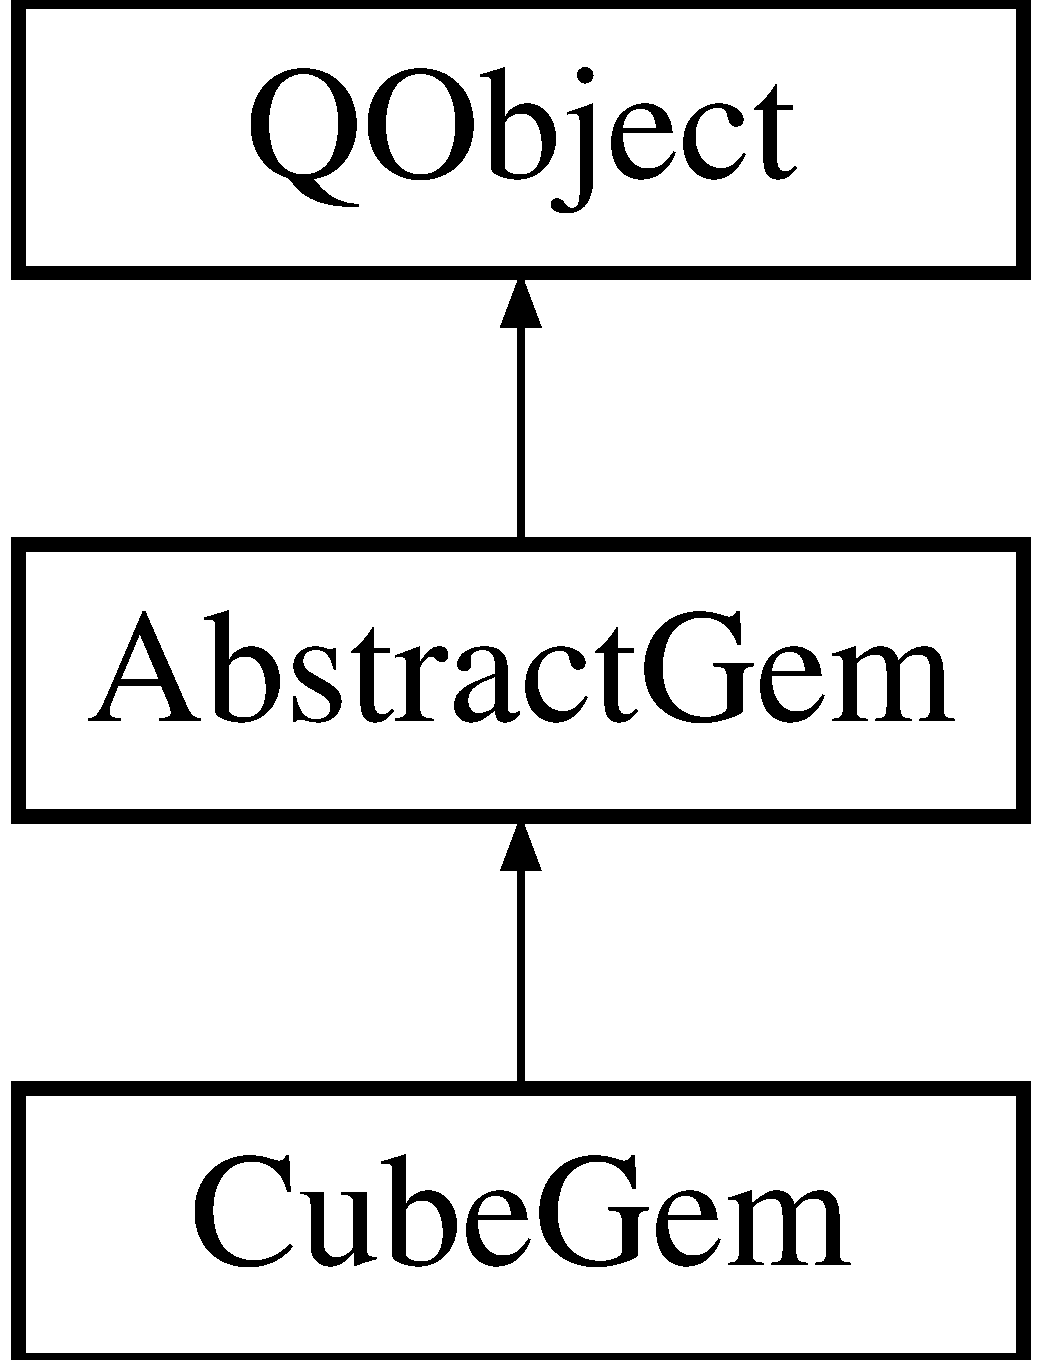
\includegraphics[height=3.000000cm]{class_cube_gem}
\end{center}
\end{figure}
\subsection*{Public Member Functions}
\begin{DoxyCompactItemize}
\item 
\hypertarget{class_cube_gem_a049ed1f21d75e2876cbbc69c56db93c2}{}{\bfseries Cube\+Gem} (Q\+Object $\ast$parent=0)\label{class_cube_gem_a049ed1f21d75e2876cbbc69c56db93c2}

\end{DoxyCompactItemize}
\subsection*{Additional Inherited Members}


The documentation for this class was generated from the following files\+:\begin{DoxyCompactItemize}
\item 
gem\+Illuminator/cubegem.\+h\item 
gem\+Illuminator/cubegem.\+cpp\end{DoxyCompactItemize}

\hypertarget{class_cube_map}{\section{Cube\+Map Class Reference}
\label{class_cube_map}\index{Cube\+Map@{Cube\+Map}}
}


The \hyperlink{class_cube_map}{Cube\+Map} class loads cubemap textures and provides them as Open\+G\+L-\/texture.  




{\ttfamily \#include $<$cubemap.\+h$>$}

Inheritance diagram for Cube\+Map\+:\begin{figure}[H]
\begin{center}
\leavevmode
\includegraphics[height=2.000000cm]{class_cube_map}
\end{center}
\end{figure}
\subsection*{Public Member Functions}
\begin{DoxyCompactItemize}
\item 
\hyperlink{class_cube_map_ac1b76abb3b551a933b23f31038855699}{Cube\+Map} (Q\+Open\+G\+L\+Functions \&gl, Q\+String cube\+Map\+Prefix, Q\+Object $\ast$parent=0)
\begin{DoxyCompactList}\small\item\em Creates a new \hyperlink{class_cube_map}{Cube\+Map} and loads required textures. \end{DoxyCompactList}\item 
virtual \hyperlink{class_cube_map_ac4c453248cd7022d3b268755b2dd218e}{$\sim$\+Cube\+Map} ()
\item 
void \hyperlink{class_cube_map_a5d772f8a6b43356593dc909a704354eb}{update} (Q\+String new\+Cube\+Map\+Prefix)
\begin{DoxyCompactList}\small\item\em Replaces current texture with new specified texture. \end{DoxyCompactList}\item 
uint \hyperlink{class_cube_map_a23189c7b896857a6080d1ceb1abf8e4a}{cube\+Map\+Texture} ()
\begin{DoxyCompactList}\small\item\em Open\+G\+L texture reference. \end{DoxyCompactList}\end{DoxyCompactItemize}
\subsection*{Protected Member Functions}
\begin{DoxyCompactItemize}
\item 
void \hyperlink{class_cube_map_a5194b38a4ee4352fe3bdae0c2daf9448}{initialize} ()
\end{DoxyCompactItemize}
\subsection*{Protected Attributes}
\begin{DoxyCompactItemize}
\item 
uint \hyperlink{class_cube_map_a07859b9c39b4c06f4b63e99b00ede4a6}{m\+\_\+cube\+Map}
\item 
Q\+Open\+G\+L\+Functions \& \hyperlink{class_cube_map_aab54def10539c674bd20212eea34a1f0}{m\+\_\+gl}
\item 
Q\+String \hyperlink{class_cube_map_a74ee2f47f59a87bc920c96396a7b33d5}{m\+\_\+cube\+Map\+Prefix}
\end{DoxyCompactItemize}


\subsection{Detailed Description}
The \hyperlink{class_cube_map}{Cube\+Map} class loads cubemap textures and provides them as Open\+G\+L-\/texture. 

\subsection{Constructor \& Destructor Documentation}
\hypertarget{class_cube_map_ac1b76abb3b551a933b23f31038855699}{\index{Cube\+Map@{Cube\+Map}!Cube\+Map@{Cube\+Map}}
\index{Cube\+Map@{Cube\+Map}!Cube\+Map@{Cube\+Map}}
\subsubsection[{Cube\+Map}]{\setlength{\rightskip}{0pt plus 5cm}Cube\+Map\+::\+Cube\+Map (
\begin{DoxyParamCaption}
\item[{Q\+Open\+G\+L\+Functions \&}]{gl, }
\item[{Q\+String}]{cube\+Map\+Prefix, }
\item[{Q\+Object $\ast$}]{parent = {\ttfamily 0}}
\end{DoxyParamCaption}
)}}\label{class_cube_map_ac1b76abb3b551a933b23f31038855699}


Creates a new \hyperlink{class_cube_map}{Cube\+Map} and loads required textures. 


\begin{DoxyParams}{Parameters}
{\em gl} & Q\+Open\+G\+L\+Functions that are used for all gl-\/calls \\
\hline
{\em cube\+Map\+Prefix} & The name of the cubemap. This is the filename of textures without fileextension and face suffix. \\
\hline
{\em parent} & Q\+Object-\/parent \\
\hline
\end{DoxyParams}
\hypertarget{class_cube_map_ac4c453248cd7022d3b268755b2dd218e}{\index{Cube\+Map@{Cube\+Map}!````~Cube\+Map@{$\sim$\+Cube\+Map}}
\index{````~Cube\+Map@{$\sim$\+Cube\+Map}!Cube\+Map@{Cube\+Map}}
\subsubsection[{$\sim$\+Cube\+Map}]{\setlength{\rightskip}{0pt plus 5cm}Cube\+Map\+::$\sim$\+Cube\+Map (
\begin{DoxyParamCaption}
{}
\end{DoxyParamCaption}
)\hspace{0.3cm}{\ttfamily [virtual]}}}\label{class_cube_map_ac4c453248cd7022d3b268755b2dd218e}


\subsection{Member Function Documentation}
\hypertarget{class_cube_map_a23189c7b896857a6080d1ceb1abf8e4a}{\index{Cube\+Map@{Cube\+Map}!cube\+Map\+Texture@{cube\+Map\+Texture}}
\index{cube\+Map\+Texture@{cube\+Map\+Texture}!Cube\+Map@{Cube\+Map}}
\subsubsection[{cube\+Map\+Texture}]{\setlength{\rightskip}{0pt plus 5cm}uint Cube\+Map\+::cube\+Map\+Texture (
\begin{DoxyParamCaption}
{}
\end{DoxyParamCaption}
)}}\label{class_cube_map_a23189c7b896857a6080d1ceb1abf8e4a}


Open\+G\+L texture reference. 

\begin{DoxyReturn}{Returns}

\end{DoxyReturn}
\hypertarget{class_cube_map_a5194b38a4ee4352fe3bdae0c2daf9448}{\index{Cube\+Map@{Cube\+Map}!initialize@{initialize}}
\index{initialize@{initialize}!Cube\+Map@{Cube\+Map}}
\subsubsection[{initialize}]{\setlength{\rightskip}{0pt plus 5cm}void Cube\+Map\+::initialize (
\begin{DoxyParamCaption}
{}
\end{DoxyParamCaption}
)\hspace{0.3cm}{\ttfamily [protected]}}}\label{class_cube_map_a5194b38a4ee4352fe3bdae0c2daf9448}
\hypertarget{class_cube_map_a5d772f8a6b43356593dc909a704354eb}{\index{Cube\+Map@{Cube\+Map}!update@{update}}
\index{update@{update}!Cube\+Map@{Cube\+Map}}
\subsubsection[{update}]{\setlength{\rightskip}{0pt plus 5cm}void Cube\+Map\+::update (
\begin{DoxyParamCaption}
\item[{Q\+String}]{new\+Cube\+Map\+Prefix}
\end{DoxyParamCaption}
)}}\label{class_cube_map_a5d772f8a6b43356593dc909a704354eb}


Replaces current texture with new specified texture. 


\begin{DoxyParams}{Parameters}
{\em new\+Cube\+Map\+Prefix} & The name of the new cubemap. This is the filename of textures without fileextension and face suffix. \\
\hline
\end{DoxyParams}


\subsection{Member Data Documentation}
\hypertarget{class_cube_map_a07859b9c39b4c06f4b63e99b00ede4a6}{\index{Cube\+Map@{Cube\+Map}!m\+\_\+cube\+Map@{m\+\_\+cube\+Map}}
\index{m\+\_\+cube\+Map@{m\+\_\+cube\+Map}!Cube\+Map@{Cube\+Map}}
\subsubsection[{m\+\_\+cube\+Map}]{\setlength{\rightskip}{0pt plus 5cm}uint Cube\+Map\+::m\+\_\+cube\+Map\hspace{0.3cm}{\ttfamily [protected]}}}\label{class_cube_map_a07859b9c39b4c06f4b63e99b00ede4a6}
\hypertarget{class_cube_map_a74ee2f47f59a87bc920c96396a7b33d5}{\index{Cube\+Map@{Cube\+Map}!m\+\_\+cube\+Map\+Prefix@{m\+\_\+cube\+Map\+Prefix}}
\index{m\+\_\+cube\+Map\+Prefix@{m\+\_\+cube\+Map\+Prefix}!Cube\+Map@{Cube\+Map}}
\subsubsection[{m\+\_\+cube\+Map\+Prefix}]{\setlength{\rightskip}{0pt plus 5cm}Q\+String Cube\+Map\+::m\+\_\+cube\+Map\+Prefix\hspace{0.3cm}{\ttfamily [protected]}}}\label{class_cube_map_a74ee2f47f59a87bc920c96396a7b33d5}
\hypertarget{class_cube_map_aab54def10539c674bd20212eea34a1f0}{\index{Cube\+Map@{Cube\+Map}!m\+\_\+gl@{m\+\_\+gl}}
\index{m\+\_\+gl@{m\+\_\+gl}!Cube\+Map@{Cube\+Map}}
\subsubsection[{m\+\_\+gl}]{\setlength{\rightskip}{0pt plus 5cm}Q\+Open\+G\+L\+Functions\& Cube\+Map\+::m\+\_\+gl\hspace{0.3cm}{\ttfamily [protected]}}}\label{class_cube_map_aab54def10539c674bd20212eea34a1f0}


The documentation for this class was generated from the following files\+:\begin{DoxyCompactItemize}
\item 
\hyperlink{cubemap_8h}{cubemap.\+h}\item 
\hyperlink{cubemap_8cpp}{cubemap.\+cpp}\end{DoxyCompactItemize}

\hypertarget{class_environment_map}{}\section{Environment\+Map Class Reference}
\label{class_environment_map}\index{Environment\+Map@{Environment\+Map}}


The \hyperlink{class_environment_map}{Environment\+Map} is a \hyperlink{class_cube_map}{Cube\+Map} based rendering technique for showing some scene enviroment.  




{\ttfamily \#include $<$environmentmap.\+h$>$}

Inheritance diagram for Environment\+Map\+:\begin{figure}[H]
\begin{center}
\leavevmode
\includegraphics[height=2.000000cm]{class_environment_map}
\end{center}
\end{figure}
\subsection*{Public Member Functions}
\begin{DoxyCompactItemize}
\item 
\hyperlink{class_environment_map_a54b674f88e757c7293abd2f52f518183}{Environment\+Map} (Q\+Open\+G\+L\+Functions \&gl, Q\+String cube\+Map\+Prefix, Q\+Object $\ast$parent=0)
\begin{DoxyCompactList}\small\item\em Creates a new \hyperlink{class_environment_map}{Environment\+Map}. The specified cube map textures are loaded imedetly(?). \end{DoxyCompactList}\item 
\hyperlink{class_environment_map_a77218340957b486754db0ff73f37c8da}{$\sim$\+Environment\+Map} ()
\item 
void \hyperlink{class_environment_map_a49b3996bb58c2e39befdea946402bbdd}{paint} (const \hyperlink{class_camera}{Camera} \&camera)
\begin{DoxyCompactList}\small\item\em Paints environmentmap into the scene using a \hyperlink{class_screen_aligned_quad}{Screen\+Aligned\+Quad}. \end{DoxyCompactList}\item 
void \hyperlink{class_environment_map_a700a5d20db46b88e2ad09675cfeb5a7f}{update} (Q\+String new\+Cube\+Map\+Prefix)
\begin{DoxyCompactList}\small\item\em Replace current \hyperlink{class_cube_map}{Cube\+Map} with new one specified by name. \end{DoxyCompactList}\item 
uint \hyperlink{class_environment_map_a49de5c6028aaf39124e6f6177aeff3db}{cube\+Map\+Texture} ()
\begin{DoxyCompactList}\small\item\em Open\+G\+L texture that is used for drawing. \end{DoxyCompactList}\end{DoxyCompactItemize}
\subsection*{Protected Member Functions}
\begin{DoxyCompactItemize}
\item 
void \hyperlink{class_environment_map_a718a9c79e383200989d22a580520fe80}{initialize} ()
\item 
void \hyperlink{class_environment_map_af348237ba84d4ac5ca45448b4a605357}{initialize\+Shader\+Program} ()
\end{DoxyCompactItemize}
\subsection*{Protected Attributes}
\begin{DoxyCompactItemize}
\item 
\hyperlink{class_cube_map}{Cube\+Map} $\ast$ \hyperlink{class_environment_map_a71fa459b1a6a88e3590cd38109bfc912}{m\+\_\+cube\+Map}
\item 
bool \hyperlink{class_environment_map_af40184d2ae6b58e909fd3c6bf1c32284}{m\+\_\+initialized}
\item 
Q\+Open\+G\+L\+Functions \& \hyperlink{class_environment_map_ad55c368a6c119293a62818a89c80da0a}{m\+\_\+gl}
\item 
\hyperlink{class_screen_aligned_quad}{Screen\+Aligned\+Quad} $\ast$ \hyperlink{class_environment_map_a2d4e6cabcbc17b659bf6dbc68069767c}{m\+\_\+quad}
\item 
Q\+Open\+G\+L\+Shader\+Program $\ast$ \hyperlink{class_environment_map_aab51ee095ecbe9fcaab64d5c8d3b3ab3}{m\+\_\+shader\+Program}
\end{DoxyCompactItemize}


\subsection{Detailed Description}
The \hyperlink{class_environment_map}{Environment\+Map} is a \hyperlink{class_cube_map}{Cube\+Map} based rendering technique for showing some scene enviroment. 

\subsection{Constructor \& Destructor Documentation}
\hypertarget{class_environment_map_a54b674f88e757c7293abd2f52f518183}{}\index{Environment\+Map@{Environment\+Map}!Environment\+Map@{Environment\+Map}}
\index{Environment\+Map@{Environment\+Map}!Environment\+Map@{Environment\+Map}}
\subsubsection[{Environment\+Map}]{\setlength{\rightskip}{0pt plus 5cm}Environment\+Map\+::\+Environment\+Map (
\begin{DoxyParamCaption}
\item[{Q\+Open\+G\+L\+Functions \&}]{gl, }
\item[{Q\+String}]{cube\+Map\+Prefix, }
\item[{Q\+Object $\ast$}]{parent = {\ttfamily 0}}
\end{DoxyParamCaption}
)}\label{class_environment_map_a54b674f88e757c7293abd2f52f518183}


Creates a new \hyperlink{class_environment_map}{Environment\+Map}. The specified cube map textures are loaded imedetly(?). 


\begin{DoxyParams}{Parameters}
{\em gl} & The Q\+Open\+G\+L\+Functions which are used for every gl-\/call \\
\hline
{\em cube\+Map\+Prefix} & The name of cubemap that should be shown. \\
\hline
{\em parent} & Q\+Object-\/parent \\
\hline
\end{DoxyParams}
\hypertarget{class_environment_map_a77218340957b486754db0ff73f37c8da}{}\index{Environment\+Map@{Environment\+Map}!````~Environment\+Map@{$\sim$\+Environment\+Map}}
\index{````~Environment\+Map@{$\sim$\+Environment\+Map}!Environment\+Map@{Environment\+Map}}
\subsubsection[{$\sim$\+Environment\+Map}]{\setlength{\rightskip}{0pt plus 5cm}Environment\+Map\+::$\sim$\+Environment\+Map (
\begin{DoxyParamCaption}
{}
\end{DoxyParamCaption}
)}\label{class_environment_map_a77218340957b486754db0ff73f37c8da}


\subsection{Member Function Documentation}
\hypertarget{class_environment_map_a49de5c6028aaf39124e6f6177aeff3db}{}\index{Environment\+Map@{Environment\+Map}!cube\+Map\+Texture@{cube\+Map\+Texture}}
\index{cube\+Map\+Texture@{cube\+Map\+Texture}!Environment\+Map@{Environment\+Map}}
\subsubsection[{cube\+Map\+Texture}]{\setlength{\rightskip}{0pt plus 5cm}uint Environment\+Map\+::cube\+Map\+Texture (
\begin{DoxyParamCaption}
{}
\end{DoxyParamCaption}
)}\label{class_environment_map_a49de5c6028aaf39124e6f6177aeff3db}


Open\+G\+L texture that is used for drawing. 

\begin{DoxyReturn}{Returns}

\end{DoxyReturn}
\hypertarget{class_environment_map_a718a9c79e383200989d22a580520fe80}{}\index{Environment\+Map@{Environment\+Map}!initialize@{initialize}}
\index{initialize@{initialize}!Environment\+Map@{Environment\+Map}}
\subsubsection[{initialize}]{\setlength{\rightskip}{0pt plus 5cm}void Environment\+Map\+::initialize (
\begin{DoxyParamCaption}
{}
\end{DoxyParamCaption}
)\hspace{0.3cm}{\ttfamily [protected]}}\label{class_environment_map_a718a9c79e383200989d22a580520fe80}
\hypertarget{class_environment_map_af348237ba84d4ac5ca45448b4a605357}{}\index{Environment\+Map@{Environment\+Map}!initialize\+Shader\+Program@{initialize\+Shader\+Program}}
\index{initialize\+Shader\+Program@{initialize\+Shader\+Program}!Environment\+Map@{Environment\+Map}}
\subsubsection[{initialize\+Shader\+Program}]{\setlength{\rightskip}{0pt plus 5cm}void Environment\+Map\+::initialize\+Shader\+Program (
\begin{DoxyParamCaption}
{}
\end{DoxyParamCaption}
)\hspace{0.3cm}{\ttfamily [protected]}}\label{class_environment_map_af348237ba84d4ac5ca45448b4a605357}
\hypertarget{class_environment_map_a49b3996bb58c2e39befdea946402bbdd}{}\index{Environment\+Map@{Environment\+Map}!paint@{paint}}
\index{paint@{paint}!Environment\+Map@{Environment\+Map}}
\subsubsection[{paint}]{\setlength{\rightskip}{0pt plus 5cm}void Environment\+Map\+::paint (
\begin{DoxyParamCaption}
\item[{const {\bf Camera} \&}]{camera}
\end{DoxyParamCaption}
)}\label{class_environment_map_a49b3996bb58c2e39befdea946402bbdd}


Paints environmentmap into the scene using a \hyperlink{class_screen_aligned_quad}{Screen\+Aligned\+Quad}. 


\begin{DoxyParams}{Parameters}
{\em camera} & The camera which is used to render the scene \\
\hline
\end{DoxyParams}
\hypertarget{class_environment_map_a700a5d20db46b88e2ad09675cfeb5a7f}{}\index{Environment\+Map@{Environment\+Map}!update@{update}}
\index{update@{update}!Environment\+Map@{Environment\+Map}}
\subsubsection[{update}]{\setlength{\rightskip}{0pt plus 5cm}void Environment\+Map\+::update (
\begin{DoxyParamCaption}
\item[{Q\+String}]{new\+Cube\+Map\+Prefix}
\end{DoxyParamCaption}
)}\label{class_environment_map_a700a5d20db46b88e2ad09675cfeb5a7f}


Replace current \hyperlink{class_cube_map}{Cube\+Map} with new one specified by name. 


\begin{DoxyParams}{Parameters}
{\em new\+Cube\+Map\+Prefix} & The name of the \hyperlink{class_cube_map}{Cube\+Map} \\
\hline
\end{DoxyParams}
\begin{DoxySeeAlso}{See also}
\hyperlink{class_cube_map_a5d772f8a6b43356593dc909a704354eb}{Cube\+Map\+::update()} 
\end{DoxySeeAlso}


\subsection{Member Data Documentation}
\hypertarget{class_environment_map_a71fa459b1a6a88e3590cd38109bfc912}{}\index{Environment\+Map@{Environment\+Map}!m\+\_\+cube\+Map@{m\+\_\+cube\+Map}}
\index{m\+\_\+cube\+Map@{m\+\_\+cube\+Map}!Environment\+Map@{Environment\+Map}}
\subsubsection[{m\+\_\+cube\+Map}]{\setlength{\rightskip}{0pt plus 5cm}{\bf Cube\+Map}$\ast$ Environment\+Map\+::m\+\_\+cube\+Map\hspace{0.3cm}{\ttfamily [protected]}}\label{class_environment_map_a71fa459b1a6a88e3590cd38109bfc912}
\hypertarget{class_environment_map_ad55c368a6c119293a62818a89c80da0a}{}\index{Environment\+Map@{Environment\+Map}!m\+\_\+gl@{m\+\_\+gl}}
\index{m\+\_\+gl@{m\+\_\+gl}!Environment\+Map@{Environment\+Map}}
\subsubsection[{m\+\_\+gl}]{\setlength{\rightskip}{0pt plus 5cm}Q\+Open\+G\+L\+Functions\& Environment\+Map\+::m\+\_\+gl\hspace{0.3cm}{\ttfamily [protected]}}\label{class_environment_map_ad55c368a6c119293a62818a89c80da0a}
\hypertarget{class_environment_map_af40184d2ae6b58e909fd3c6bf1c32284}{}\index{Environment\+Map@{Environment\+Map}!m\+\_\+initialized@{m\+\_\+initialized}}
\index{m\+\_\+initialized@{m\+\_\+initialized}!Environment\+Map@{Environment\+Map}}
\subsubsection[{m\+\_\+initialized}]{\setlength{\rightskip}{0pt plus 5cm}bool Environment\+Map\+::m\+\_\+initialized\hspace{0.3cm}{\ttfamily [protected]}}\label{class_environment_map_af40184d2ae6b58e909fd3c6bf1c32284}
\hypertarget{class_environment_map_a2d4e6cabcbc17b659bf6dbc68069767c}{}\index{Environment\+Map@{Environment\+Map}!m\+\_\+quad@{m\+\_\+quad}}
\index{m\+\_\+quad@{m\+\_\+quad}!Environment\+Map@{Environment\+Map}}
\subsubsection[{m\+\_\+quad}]{\setlength{\rightskip}{0pt plus 5cm}{\bf Screen\+Aligned\+Quad}$\ast$ Environment\+Map\+::m\+\_\+quad\hspace{0.3cm}{\ttfamily [protected]}}\label{class_environment_map_a2d4e6cabcbc17b659bf6dbc68069767c}
\hypertarget{class_environment_map_aab51ee095ecbe9fcaab64d5c8d3b3ab3}{}\index{Environment\+Map@{Environment\+Map}!m\+\_\+shader\+Program@{m\+\_\+shader\+Program}}
\index{m\+\_\+shader\+Program@{m\+\_\+shader\+Program}!Environment\+Map@{Environment\+Map}}
\subsubsection[{m\+\_\+shader\+Program}]{\setlength{\rightskip}{0pt plus 5cm}Q\+Open\+G\+L\+Shader\+Program$\ast$ Environment\+Map\+::m\+\_\+shader\+Program\hspace{0.3cm}{\ttfamily [protected]}}\label{class_environment_map_aab51ee095ecbe9fcaab64d5c8d3b3ab3}


The documentation for this class was generated from the following files\+:\begin{DoxyCompactItemize}
\item 
Game-\/\+Programming-\/\+W\+S2014/gem\+Illuminator/\hyperlink{environmentmap_8h}{environmentmap.\+h}\item 
Game-\/\+Programming-\/\+W\+S2014/gem\+Illuminator/\hyperlink{environmentmap_8cpp}{environmentmap.\+cpp}\end{DoxyCompactItemize}

\hypertarget{class_file_i_o}{}\section{File\+I\+O Class Reference}
\label{class_file_i_o}\index{File\+I\+O@{File\+I\+O}}


The \hyperlink{class_file_i_o}{File\+I\+O} class provides platform independent file reading for ressource files used by us.  The file that should be read is specified by name and \hyperlink{class_file_i_o}{File\+I\+O} will load it from platform dependent location.  




{\ttfamily \#include $<$fileio.\+h$>$}

Inheritance diagram for File\+I\+O\+:\begin{figure}[H]
\begin{center}
\leavevmode
\includegraphics[height=3.000000cm]{class_file_i_o}
\end{center}
\end{figure}
\subsection*{Signals}
\begin{DoxyCompactItemize}
\item 
void \hyperlink{class_file_i_o_a4136bb085d530f9dd54eb849f14d58da}{error} (const Q\+String \&msg)
\begin{DoxyCompactList}\small\item\em This signal will be emitted if an error occurs. \end{DoxyCompactList}\item 
void \hyperlink{class_file_i_o_a31a6e00e907268e4473a0a826d2e6a1e}{source\+Changed} (const Q\+String \&\hyperlink{class_file_i_o_ad4467aa6c50748ac1e7076d25dcd33cc}{source})
\begin{DoxyCompactList}\small\item\em This signal is emitted if the \hyperlink{class_file_i_o_a8da2b4c6cd72af512e4556203c1c66e7}{source()} is changed. \end{DoxyCompactList}\end{DoxyCompactItemize}
\subsection*{Public Member Functions}
\begin{DoxyCompactItemize}
\item 
\hyperlink{class_file_i_o_a6e4f7122f89b633e3522c2e1d31e1fdd}{File\+I\+O} (Q\+Object $\ast$parent=0)
\begin{DoxyCompactList}\small\item\em Creates a new \hyperlink{class_file_i_o}{File\+I\+O}. \end{DoxyCompactList}\item 
\hyperlink{class_file_i_o_adc3caa8f1e5d76274d8ffb8b5c17288b}{$\sim$\+File\+I\+O} ()
\item 
Q\+\_\+\+I\+N\+V\+O\+K\+A\+B\+L\+E Q\+String \hyperlink{class_file_i_o_a48c90efc3bf8dda4d612f2dff5409834}{read} ()
\begin{DoxyCompactList}\small\item\em Reads previous specified file. \end{DoxyCompactList}\item 
void \hyperlink{class_file_i_o_a985a2cce4d400bca160c5f42bf697adb}{set\+Source} (const Q\+String \&\hyperlink{class_file_i_o_ad4467aa6c50748ac1e7076d25dcd33cc}{source})
\begin{DoxyCompactList}\small\item\em Sets the source file by name. The source is read calling \hyperlink{class_file_i_o_a48c90efc3bf8dda4d612f2dff5409834}{read()} \end{DoxyCompactList}\item 
Q\+String \hyperlink{class_file_i_o_a8da2b4c6cd72af512e4556203c1c66e7}{source} ()
\begin{DoxyCompactList}\small\item\em The name of file that is read by \hyperlink{class_file_i_o_a48c90efc3bf8dda4d612f2dff5409834}{read()}. \end{DoxyCompactList}\item 
Q\+\_\+\+I\+N\+V\+O\+K\+A\+B\+L\+E bool \hyperlink{class_file_i_o_a73bc6cac958f024325e795a690740a85}{write} (const Q\+String \&data)
\begin{DoxyCompactList}\small\item\em Writes specified data into \hyperlink{class_file_i_o_a8da2b4c6cd72af512e4556203c1c66e7}{source()} \end{DoxyCompactList}\end{DoxyCompactItemize}
\subsection*{Protected Attributes}
\begin{DoxyCompactItemize}
\item 
Q\+String \hyperlink{class_file_i_o_ab8f8edbc97eec6d3cf77e314a8754ef3}{m\+\_\+source}
\end{DoxyCompactItemize}
\subsection*{Properties}
\begin{DoxyCompactItemize}
\item 
Q\+String \hyperlink{class_file_i_o_ad4467aa6c50748ac1e7076d25dcd33cc}{source}
\end{DoxyCompactItemize}


\subsection{Detailed Description}
The \hyperlink{class_file_i_o}{File\+I\+O} class provides platform independent file reading for ressource files used by us.  The file that should be read is specified by name and \hyperlink{class_file_i_o}{File\+I\+O} will load it from platform dependent location. 

\subsection{Constructor \& Destructor Documentation}
\hypertarget{class_file_i_o_a6e4f7122f89b633e3522c2e1d31e1fdd}{}\index{File\+I\+O@{File\+I\+O}!File\+I\+O@{File\+I\+O}}
\index{File\+I\+O@{File\+I\+O}!File\+I\+O@{File\+I\+O}}
\subsubsection[{File\+I\+O}]{\setlength{\rightskip}{0pt plus 5cm}File\+I\+O\+::\+File\+I\+O (
\begin{DoxyParamCaption}
\item[{Q\+Object $\ast$}]{parent = {\ttfamily 0}}
\end{DoxyParamCaption}
)\hspace{0.3cm}{\ttfamily [explicit]}}\label{class_file_i_o_a6e4f7122f89b633e3522c2e1d31e1fdd}


Creates a new \hyperlink{class_file_i_o}{File\+I\+O}. 


\begin{DoxyParams}{Parameters}
{\em parent} & Q\+Object-\/parent \\
\hline
\end{DoxyParams}
\hypertarget{class_file_i_o_adc3caa8f1e5d76274d8ffb8b5c17288b}{}\index{File\+I\+O@{File\+I\+O}!````~File\+I\+O@{$\sim$\+File\+I\+O}}
\index{````~File\+I\+O@{$\sim$\+File\+I\+O}!File\+I\+O@{File\+I\+O}}
\subsubsection[{$\sim$\+File\+I\+O}]{\setlength{\rightskip}{0pt plus 5cm}File\+I\+O\+::$\sim$\+File\+I\+O (
\begin{DoxyParamCaption}
{}
\end{DoxyParamCaption}
)}\label{class_file_i_o_adc3caa8f1e5d76274d8ffb8b5c17288b}


\subsection{Member Function Documentation}
\hypertarget{class_file_i_o_a4136bb085d530f9dd54eb849f14d58da}{}\index{File\+I\+O@{File\+I\+O}!error@{error}}
\index{error@{error}!File\+I\+O@{File\+I\+O}}
\subsubsection[{error}]{\setlength{\rightskip}{0pt plus 5cm}void File\+I\+O\+::error (
\begin{DoxyParamCaption}
\item[{const Q\+String \&}]{msg}
\end{DoxyParamCaption}
)\hspace{0.3cm}{\ttfamily [signal]}}\label{class_file_i_o_a4136bb085d530f9dd54eb849f14d58da}


This signal will be emitted if an error occurs. 


\begin{DoxyParams}{Parameters}
{\em msg} & The error message describing the error \\
\hline
\end{DoxyParams}
\hypertarget{class_file_i_o_a48c90efc3bf8dda4d612f2dff5409834}{}\index{File\+I\+O@{File\+I\+O}!read@{read}}
\index{read@{read}!File\+I\+O@{File\+I\+O}}
\subsubsection[{read}]{\setlength{\rightskip}{0pt plus 5cm}Q\+String File\+I\+O\+::read (
\begin{DoxyParamCaption}
{}
\end{DoxyParamCaption}
)}\label{class_file_i_o_a48c90efc3bf8dda4d612f2dff5409834}


Reads previous specified file. 

\begin{DoxyReturn}{Returns}
Read file as Q\+String. 
\end{DoxyReturn}
\hypertarget{class_file_i_o_a985a2cce4d400bca160c5f42bf697adb}{}\index{File\+I\+O@{File\+I\+O}!set\+Source@{set\+Source}}
\index{set\+Source@{set\+Source}!File\+I\+O@{File\+I\+O}}
\subsubsection[{set\+Source}]{\setlength{\rightskip}{0pt plus 5cm}void File\+I\+O\+::set\+Source (
\begin{DoxyParamCaption}
\item[{const Q\+String \&}]{source}
\end{DoxyParamCaption}
)}\label{class_file_i_o_a985a2cce4d400bca160c5f42bf697adb}


Sets the source file by name. The source is read calling \hyperlink{class_file_i_o_a48c90efc3bf8dda4d612f2dff5409834}{read()} 


\begin{DoxyParams}{Parameters}
{\em source} & The name of file that should be read. \\
\hline
\end{DoxyParams}
\hypertarget{class_file_i_o_a8da2b4c6cd72af512e4556203c1c66e7}{}\index{File\+I\+O@{File\+I\+O}!source@{source}}
\index{source@{source}!File\+I\+O@{File\+I\+O}}
\subsubsection[{source}]{\setlength{\rightskip}{0pt plus 5cm}Q\+String File\+I\+O\+::source (
\begin{DoxyParamCaption}
{}
\end{DoxyParamCaption}
)}\label{class_file_i_o_a8da2b4c6cd72af512e4556203c1c66e7}


The name of file that is read by \hyperlink{class_file_i_o_a48c90efc3bf8dda4d612f2dff5409834}{read()}. 

\begin{DoxyReturn}{Returns}

\end{DoxyReturn}
\hypertarget{class_file_i_o_a31a6e00e907268e4473a0a826d2e6a1e}{}\index{File\+I\+O@{File\+I\+O}!source\+Changed@{source\+Changed}}
\index{source\+Changed@{source\+Changed}!File\+I\+O@{File\+I\+O}}
\subsubsection[{source\+Changed}]{\setlength{\rightskip}{0pt plus 5cm}void File\+I\+O\+::source\+Changed (
\begin{DoxyParamCaption}
\item[{const Q\+String \&}]{source}
\end{DoxyParamCaption}
)\hspace{0.3cm}{\ttfamily [signal]}}\label{class_file_i_o_a31a6e00e907268e4473a0a826d2e6a1e}


This signal is emitted if the \hyperlink{class_file_i_o_a8da2b4c6cd72af512e4556203c1c66e7}{source()} is changed. 


\begin{DoxyParams}{Parameters}
{\em source} & The new source \\
\hline
\end{DoxyParams}
\hypertarget{class_file_i_o_a73bc6cac958f024325e795a690740a85}{}\index{File\+I\+O@{File\+I\+O}!write@{write}}
\index{write@{write}!File\+I\+O@{File\+I\+O}}
\subsubsection[{write}]{\setlength{\rightskip}{0pt plus 5cm}bool File\+I\+O\+::write (
\begin{DoxyParamCaption}
\item[{const Q\+String \&}]{data}
\end{DoxyParamCaption}
)}\label{class_file_i_o_a73bc6cac958f024325e795a690740a85}


Writes specified data into \hyperlink{class_file_i_o_a8da2b4c6cd72af512e4556203c1c66e7}{source()} 


\begin{DoxyParams}{Parameters}
{\em data} & The data that will be written into \hyperlink{class_file_i_o_a8da2b4c6cd72af512e4556203c1c66e7}{source()} \\
\hline
\end{DoxyParams}


\subsection{Member Data Documentation}
\hypertarget{class_file_i_o_ab8f8edbc97eec6d3cf77e314a8754ef3}{}\index{File\+I\+O@{File\+I\+O}!m\+\_\+source@{m\+\_\+source}}
\index{m\+\_\+source@{m\+\_\+source}!File\+I\+O@{File\+I\+O}}
\subsubsection[{m\+\_\+source}]{\setlength{\rightskip}{0pt plus 5cm}Q\+String File\+I\+O\+::m\+\_\+source\hspace{0.3cm}{\ttfamily [protected]}}\label{class_file_i_o_ab8f8edbc97eec6d3cf77e314a8754ef3}


\subsection{Property Documentation}
\hypertarget{class_file_i_o_ad4467aa6c50748ac1e7076d25dcd33cc}{}\index{File\+I\+O@{File\+I\+O}!source@{source}}
\index{source@{source}!File\+I\+O@{File\+I\+O}}
\subsubsection[{source}]{\setlength{\rightskip}{0pt plus 5cm}Q\+String File\+I\+O\+::source\hspace{0.3cm}{\ttfamily [read]}, {\ttfamily [write]}}\label{class_file_i_o_ad4467aa6c50748ac1e7076d25dcd33cc}


The documentation for this class was generated from the following files\+:\begin{DoxyCompactItemize}
\item 
Game-\/\+Programming-\/\+W\+S2014/gem\+Illuminator/\hyperlink{fileio_8h}{fileio.\+h}\item 
Game-\/\+Programming-\/\+W\+S2014/gem\+Illuminator/\hyperlink{fileio_8cpp}{fileio.\+cpp}\end{DoxyCompactItemize}

\hypertarget{class_game_lost_ray}{}\section{Game\+Lost\+Ray Class Reference}
\label{class_game_lost_ray}\index{Game\+Lost\+Ray@{Game\+Lost\+Ray}}


The \hyperlink{class_game_lost_ray}{Game\+Lost\+Ray} class is a specialized \hyperlink{class_light_ray}{Light\+Ray}, that is created if the player should loose as soon as the player reaches it.  




{\ttfamily \#include $<$gamelostray.\+h$>$}

Inheritance diagram for Game\+Lost\+Ray\+:\begin{figure}[H]
\begin{center}
\leavevmode
\includegraphics[height=3.000000cm]{class_game_lost_ray}
\end{center}
\end{figure}
\subsection*{Signals}
\begin{DoxyCompactItemize}
\item 
void \hyperlink{class_game_lost_ray_a9b2afbad70387bd9ec8f80170760ef57}{game\+Lost} ()
\begin{DoxyCompactList}\small\item\em The \hyperlink{class_game_lost_ray_a9b2afbad70387bd9ec8f80170760ef57}{game\+Lost()} signal is emitted at that moment the ray detects the player leaving the scene. \end{DoxyCompactList}\end{DoxyCompactItemize}
\subsection*{Public Member Functions}
\begin{DoxyCompactItemize}
\item 
\hyperlink{class_game_lost_ray_a15ec367ee8dfd87bc8deccde5553f8e6}{Game\+Lost\+Ray} (Q\+Object $\ast$parent=0)
\item 
void \hyperlink{class_game_lost_ray_a417d814372891fe7595a7e745b7a9f0f}{update} (int time\+Difference) override
\begin{DoxyCompactList}\small\item\em This method is like \hyperlink{class_light_ray_acf06a71a307433fa5b220baccf809e64}{Light\+Ray\+::update()} with the addition, that the game end is detect a soon as the ray has a player-\/$>$ \end{DoxyCompactList}\end{DoxyCompactItemize}
\subsection*{Protected Attributes}
\begin{DoxyCompactItemize}
\item 
bool \hyperlink{class_game_lost_ray_a9b8fd54b22a3f25d4fef9431cebafa7a}{m\+\_\+already\+Lost}
\end{DoxyCompactItemize}
\subsection*{Additional Inherited Members}


\subsection{Detailed Description}
The \hyperlink{class_game_lost_ray}{Game\+Lost\+Ray} class is a specialized \hyperlink{class_light_ray}{Light\+Ray}, that is created if the player should loose as soon as the player reaches it. 

\subsection{Constructor \& Destructor Documentation}
\hypertarget{class_game_lost_ray_a15ec367ee8dfd87bc8deccde5553f8e6}{}\index{Game\+Lost\+Ray@{Game\+Lost\+Ray}!Game\+Lost\+Ray@{Game\+Lost\+Ray}}
\index{Game\+Lost\+Ray@{Game\+Lost\+Ray}!Game\+Lost\+Ray@{Game\+Lost\+Ray}}
\subsubsection[{Game\+Lost\+Ray}]{\setlength{\rightskip}{0pt plus 5cm}Game\+Lost\+Ray\+::\+Game\+Lost\+Ray (
\begin{DoxyParamCaption}
\item[{Q\+Object $\ast$}]{parent = {\ttfamily 0}}
\end{DoxyParamCaption}
)\hspace{0.3cm}{\ttfamily [explicit]}}\label{class_game_lost_ray_a15ec367ee8dfd87bc8deccde5553f8e6}


\subsection{Member Function Documentation}
\hypertarget{class_game_lost_ray_a9b2afbad70387bd9ec8f80170760ef57}{}\index{Game\+Lost\+Ray@{Game\+Lost\+Ray}!game\+Lost@{game\+Lost}}
\index{game\+Lost@{game\+Lost}!Game\+Lost\+Ray@{Game\+Lost\+Ray}}
\subsubsection[{game\+Lost}]{\setlength{\rightskip}{0pt plus 5cm}void Game\+Lost\+Ray\+::game\+Lost (
\begin{DoxyParamCaption}
{}
\end{DoxyParamCaption}
)\hspace{0.3cm}{\ttfamily [signal]}}\label{class_game_lost_ray_a9b2afbad70387bd9ec8f80170760ef57}


The \hyperlink{class_game_lost_ray_a9b2afbad70387bd9ec8f80170760ef57}{game\+Lost()} signal is emitted at that moment the ray detects the player leaving the scene. 

\hypertarget{class_game_lost_ray_a417d814372891fe7595a7e745b7a9f0f}{}\index{Game\+Lost\+Ray@{Game\+Lost\+Ray}!update@{update}}
\index{update@{update}!Game\+Lost\+Ray@{Game\+Lost\+Ray}}
\subsubsection[{update}]{\setlength{\rightskip}{0pt plus 5cm}void Game\+Lost\+Ray\+::update (
\begin{DoxyParamCaption}
\item[{int}]{time\+Difference}
\end{DoxyParamCaption}
)\hspace{0.3cm}{\ttfamily [override]}, {\ttfamily [virtual]}}\label{class_game_lost_ray_a417d814372891fe7595a7e745b7a9f0f}


This method is like \hyperlink{class_light_ray_acf06a71a307433fa5b220baccf809e64}{Light\+Ray\+::update()} with the addition, that the game end is detect a soon as the ray has a player-\/$>$ 


\begin{DoxyParams}{Parameters}
{\em time\+Difference} & Time differnce to previous update. \\
\hline
\end{DoxyParams}


Reimplemented from \hyperlink{class_light_ray_acf06a71a307433fa5b220baccf809e64}{Light\+Ray}.



\subsection{Member Data Documentation}
\hypertarget{class_game_lost_ray_a9b8fd54b22a3f25d4fef9431cebafa7a}{}\index{Game\+Lost\+Ray@{Game\+Lost\+Ray}!m\+\_\+already\+Lost@{m\+\_\+already\+Lost}}
\index{m\+\_\+already\+Lost@{m\+\_\+already\+Lost}!Game\+Lost\+Ray@{Game\+Lost\+Ray}}
\subsubsection[{m\+\_\+already\+Lost}]{\setlength{\rightskip}{0pt plus 5cm}bool Game\+Lost\+Ray\+::m\+\_\+already\+Lost\hspace{0.3cm}{\ttfamily [protected]}}\label{class_game_lost_ray_a9b8fd54b22a3f25d4fef9431cebafa7a}


The documentation for this class was generated from the following files\+:\begin{DoxyCompactItemize}
\item 
Game-\/\+Programming-\/\+W\+S2014/gem\+Illuminator/\hyperlink{gamelostray_8h}{gamelostray.\+h}\item 
Game-\/\+Programming-\/\+W\+S2014/gem\+Illuminator/\hyperlink{gamelostray_8cpp}{gamelostray.\+cpp}\end{DoxyCompactItemize}

\hypertarget{class_gem_data}{}\section{Gem\+Data Class Reference}
\label{class_gem_data}\index{Gem\+Data@{Gem\+Data}}


The \hyperlink{class_gem_data}{Gem\+Data} class stores all required information to describe a \hyperlink{class_abstract_gem}{Abstract\+Gem}.  The adventage of \hyperlink{class_gem_data}{Gem\+Data} is, that it is possible to assign, copy, compare and \hyperlink{abstractgem_8cpp_a92fb5a3a6f53f07f0f9653dd299d31ff}{q\+Hash()} this class. Therefore it is possible to store it in most Qt-\/containers.  




{\ttfamily \#include $<$gemdata.\+h$>$}

\subsection*{Public Member Functions}
\begin{DoxyCompactItemize}
\item 
\hyperlink{class_gem_data_a1140e4a3ecf37d05cddf303d7a120ca1}{Gem\+Data} ()
\begin{DoxyCompactList}\small\item\em Creates a new \hyperlink{class_gem_data}{Gem\+Data} with all values initialized to zero. \end{DoxyCompactList}\item 
\hyperlink{class_gem_data_a384ba75fa94427e138d3f7240ffd2877}{Gem\+Data} (const \hyperlink{class_gem_data}{Gem\+Data} \&ohter\+Gem\+Data)
\begin{DoxyCompactList}\small\item\em Copy constructor. \end{DoxyCompactList}\item 
\hyperlink{class_gem_data_abbd61a573420a780baa954890b0409ea}{$\sim$\+Gem\+Data} ()
\item 
\hyperlink{class_gem_data}{Gem\+Data} \& \hyperlink{class_gem_data_a736bacc522b569d04d40321b40cabc6a}{operator=} (const \hyperlink{class_gem_data}{Gem\+Data} \&rhs)
\item 
const Q\+Vector3\+D \& \hyperlink{class_gem_data_af210f7380a31e39e1494629fb4f7b5d1}{color} () const 
\item 
void \hyperlink{class_gem_data_a08bf37ae1fa58d93146f10719c2fed41}{set\+Color} (const Q\+Vector3\+D \&\hyperlink{class_gem_data_af210f7380a31e39e1494629fb4f7b5d1}{color})
\item 
const Q\+Matrix4x4 \& \hyperlink{class_gem_data_acf4d522f8c4ef7dd30c184b73790a8fb}{model} () const 
\begin{DoxyCompactList}\small\item\em Returns on demand the modelmatrix of current gem\+Data. \end{DoxyCompactList}\item 
const Q\+Vector3\+D \& \hyperlink{class_gem_data_aa863540bdd957405b632864da28908b2}{position} () const 
\item 
void \hyperlink{class_gem_data_a6e1ea1cab5241f228842cd47b37202fa}{set\+Position} (const Q\+Vector3\+D \&\hyperlink{class_gem_data_aa863540bdd957405b632864da28908b2}{position})
\item 
const Q\+Quaternion \& \hyperlink{class_gem_data_a3c902384912903b22d5eaab7e70f1f5c}{rotation} () const 
\item 
void \hyperlink{class_gem_data_ac22fb4a6faf13d78299be0f5cfd029a1}{set\+Rotation} (const Q\+Quaternion \&\hyperlink{class_gem_data_a3c902384912903b22d5eaab7e70f1f5c}{rotation})
\item 
float \hyperlink{class_gem_data_a39ef099801a421c7b7ffbbd920084eb0}{scale} () const 
\item 
void \hyperlink{class_gem_data_a49e18ed27815f66469f4ac951b5f969b}{set\+Scale} (float \hyperlink{class_gem_data_a39ef099801a421c7b7ffbbd920084eb0}{scale})
\item 
const \hyperlink{class_q_list}{Q\+List}$<$ \hyperlink{class_triangle}{Triangle} $\ast$ $>$ \& \hyperlink{class_gem_data_a2c8956630fdf362efe4e69db9bad2f7f}{triangles} () const 
\item 
void \hyperlink{class_gem_data_aa4be4b2b96ae412308c89e053249d744}{set\+Triangles} (const \hyperlink{class_q_list}{Q\+List}$<$ \hyperlink{class_triangle}{Triangle} $\ast$ $>$ \&\hyperlink{class_gem_data_a2c8956630fdf362efe4e69db9bad2f7f}{triangles})
\item 
\hyperlink{abstractgem_8h_a2f0a34b6dac35a9610cab7a1c5fcb444}{Gem\+Type} \hyperlink{class_gem_data_a38e33b0c64c37f30d0e063580d6a20bb}{type} () const 
\item 
void \hyperlink{class_gem_data_a10d94a0bd72a57fb9a52a8f534f3e1dd}{set\+Type} (\hyperlink{abstractgem_8h_a2f0a34b6dac35a9610cab7a1c5fcb444}{Gem\+Type} \hyperlink{class_gem_data_a38e33b0c64c37f30d0e063580d6a20bb}{type})
\end{DoxyCompactItemize}
\subsection*{Protected Member Functions}
\begin{DoxyCompactItemize}
\item 
void \hyperlink{class_gem_data_a24986c8eaaa23640a7cb7fff9f4df2b5}{copy\+Triangles} (const \hyperlink{class_q_list}{Q\+List}$<$ \hyperlink{class_triangle}{Triangle} $\ast$ $>$ \&\hyperlink{class_gem_data_a2c8956630fdf362efe4e69db9bad2f7f}{triangles})
\item 
void \hyperlink{class_gem_data_ac558e3bbb71c2ec73400f0a0cb309693}{calculate\+Model\+Matrix} () const 
\end{DoxyCompactItemize}
\subsection*{Protected Attributes}
\begin{DoxyCompactItemize}
\item 
Q\+Vector3\+D $\ast$ \hyperlink{class_gem_data_aa5888d4d3212ba621643a0f1c1efca76}{m\+\_\+color}
\item 
bool \hyperlink{class_gem_data_a82ba26b9a691149c8525244969cceaef}{m\+\_\+is\+Model\+Invalid}
\item 
Q\+Matrix4x4 $\ast$ \hyperlink{class_gem_data_a3a7eec529b0228a410ea608401cf2f1a}{m\+\_\+model}
\item 
Q\+Vector3\+D $\ast$ \hyperlink{class_gem_data_ad5c2bc9fc38c168fbbf143e0092c8cdb}{m\+\_\+position}
\item 
Q\+Quaternion $\ast$ \hyperlink{class_gem_data_a8a055b766496fa47842a683035f15637}{m\+\_\+rotation}
\item 
float \hyperlink{class_gem_data_a15953642fe15a2a37aceea037e4ad81e}{m\+\_\+scale}
\item 
\hyperlink{class_q_list}{Q\+List}$<$ \hyperlink{class_triangle}{Triangle} $\ast$ $>$ $\ast$ \hyperlink{class_gem_data_a21068b04db70d2e37e9c30d816484f25}{m\+\_\+triangles}
\item 
\hyperlink{abstractgem_8h_a2f0a34b6dac35a9610cab7a1c5fcb444}{Gem\+Type} \hyperlink{class_gem_data_a310940114f54b2146f6601662e8a323f}{m\+\_\+type}
\end{DoxyCompactItemize}


\subsection{Detailed Description}
The \hyperlink{class_gem_data}{Gem\+Data} class stores all required information to describe a \hyperlink{class_abstract_gem}{Abstract\+Gem}.  The adventage of \hyperlink{class_gem_data}{Gem\+Data} is, that it is possible to assign, copy, compare and \hyperlink{abstractgem_8cpp_a92fb5a3a6f53f07f0f9653dd299d31ff}{q\+Hash()} this class. Therefore it is possible to store it in most Qt-\/containers. 

\subsection{Constructor \& Destructor Documentation}
\hypertarget{class_gem_data_a1140e4a3ecf37d05cddf303d7a120ca1}{}\index{Gem\+Data@{Gem\+Data}!Gem\+Data@{Gem\+Data}}
\index{Gem\+Data@{Gem\+Data}!Gem\+Data@{Gem\+Data}}
\subsubsection[{Gem\+Data}]{\setlength{\rightskip}{0pt plus 5cm}Gem\+Data\+::\+Gem\+Data (
\begin{DoxyParamCaption}
{}
\end{DoxyParamCaption}
)}\label{class_gem_data_a1140e4a3ecf37d05cddf303d7a120ca1}


Creates a new \hyperlink{class_gem_data}{Gem\+Data} with all values initialized to zero. 

\hypertarget{class_gem_data_a384ba75fa94427e138d3f7240ffd2877}{}\index{Gem\+Data@{Gem\+Data}!Gem\+Data@{Gem\+Data}}
\index{Gem\+Data@{Gem\+Data}!Gem\+Data@{Gem\+Data}}
\subsubsection[{Gem\+Data}]{\setlength{\rightskip}{0pt plus 5cm}Gem\+Data\+::\+Gem\+Data (
\begin{DoxyParamCaption}
\item[{const {\bf Gem\+Data} \&}]{ohter\+Gem\+Data}
\end{DoxyParamCaption}
)}\label{class_gem_data_a384ba75fa94427e138d3f7240ffd2877}


Copy constructor. 


\begin{DoxyParams}{Parameters}
{\em ohter\+Gem\+Data} & \hyperlink{class_gem_data}{Gem\+Data} that should be copied. \\
\hline
\end{DoxyParams}
\hypertarget{class_gem_data_abbd61a573420a780baa954890b0409ea}{}\index{Gem\+Data@{Gem\+Data}!````~Gem\+Data@{$\sim$\+Gem\+Data}}
\index{````~Gem\+Data@{$\sim$\+Gem\+Data}!Gem\+Data@{Gem\+Data}}
\subsubsection[{$\sim$\+Gem\+Data}]{\setlength{\rightskip}{0pt plus 5cm}Gem\+Data\+::$\sim$\+Gem\+Data (
\begin{DoxyParamCaption}
{}
\end{DoxyParamCaption}
)}\label{class_gem_data_abbd61a573420a780baa954890b0409ea}


\subsection{Member Function Documentation}
\hypertarget{class_gem_data_ac558e3bbb71c2ec73400f0a0cb309693}{}\index{Gem\+Data@{Gem\+Data}!calculate\+Model\+Matrix@{calculate\+Model\+Matrix}}
\index{calculate\+Model\+Matrix@{calculate\+Model\+Matrix}!Gem\+Data@{Gem\+Data}}
\subsubsection[{calculate\+Model\+Matrix}]{\setlength{\rightskip}{0pt plus 5cm}void Gem\+Data\+::calculate\+Model\+Matrix (
\begin{DoxyParamCaption}
{}
\end{DoxyParamCaption}
) const\hspace{0.3cm}{\ttfamily [protected]}}\label{class_gem_data_ac558e3bbb71c2ec73400f0a0cb309693}
\hypertarget{class_gem_data_af210f7380a31e39e1494629fb4f7b5d1}{}\index{Gem\+Data@{Gem\+Data}!color@{color}}
\index{color@{color}!Gem\+Data@{Gem\+Data}}
\subsubsection[{color}]{\setlength{\rightskip}{0pt plus 5cm}const Q\+Vector3\+D \& Gem\+Data\+::color (
\begin{DoxyParamCaption}
{}
\end{DoxyParamCaption}
) const}\label{class_gem_data_af210f7380a31e39e1494629fb4f7b5d1}
\hypertarget{class_gem_data_a24986c8eaaa23640a7cb7fff9f4df2b5}{}\index{Gem\+Data@{Gem\+Data}!copy\+Triangles@{copy\+Triangles}}
\index{copy\+Triangles@{copy\+Triangles}!Gem\+Data@{Gem\+Data}}
\subsubsection[{copy\+Triangles}]{\setlength{\rightskip}{0pt plus 5cm}void Gem\+Data\+::copy\+Triangles (
\begin{DoxyParamCaption}
\item[{const {\bf Q\+List}$<$ {\bf Triangle} $\ast$ $>$ \&}]{triangles}
\end{DoxyParamCaption}
)\hspace{0.3cm}{\ttfamily [protected]}}\label{class_gem_data_a24986c8eaaa23640a7cb7fff9f4df2b5}
\hypertarget{class_gem_data_acf4d522f8c4ef7dd30c184b73790a8fb}{}\index{Gem\+Data@{Gem\+Data}!model@{model}}
\index{model@{model}!Gem\+Data@{Gem\+Data}}
\subsubsection[{model}]{\setlength{\rightskip}{0pt plus 5cm}const Q\+Matrix4x4 \& Gem\+Data\+::model (
\begin{DoxyParamCaption}
{}
\end{DoxyParamCaption}
) const}\label{class_gem_data_acf4d522f8c4ef7dd30c184b73790a8fb}


Returns on demand the modelmatrix of current gem\+Data. 

\begin{DoxyReturn}{Returns}

\end{DoxyReturn}
\hypertarget{class_gem_data_a736bacc522b569d04d40321b40cabc6a}{}\index{Gem\+Data@{Gem\+Data}!operator=@{operator=}}
\index{operator=@{operator=}!Gem\+Data@{Gem\+Data}}
\subsubsection[{operator=}]{\setlength{\rightskip}{0pt plus 5cm}{\bf Gem\+Data} \& Gem\+Data\+::operator= (
\begin{DoxyParamCaption}
\item[{const {\bf Gem\+Data} \&}]{rhs}
\end{DoxyParamCaption}
)}\label{class_gem_data_a736bacc522b569d04d40321b40cabc6a}
\hypertarget{class_gem_data_aa863540bdd957405b632864da28908b2}{}\index{Gem\+Data@{Gem\+Data}!position@{position}}
\index{position@{position}!Gem\+Data@{Gem\+Data}}
\subsubsection[{position}]{\setlength{\rightskip}{0pt plus 5cm}const Q\+Vector3\+D \& Gem\+Data\+::position (
\begin{DoxyParamCaption}
{}
\end{DoxyParamCaption}
) const}\label{class_gem_data_aa863540bdd957405b632864da28908b2}
\hypertarget{class_gem_data_a3c902384912903b22d5eaab7e70f1f5c}{}\index{Gem\+Data@{Gem\+Data}!rotation@{rotation}}
\index{rotation@{rotation}!Gem\+Data@{Gem\+Data}}
\subsubsection[{rotation}]{\setlength{\rightskip}{0pt plus 5cm}const Q\+Quaternion \& Gem\+Data\+::rotation (
\begin{DoxyParamCaption}
{}
\end{DoxyParamCaption}
) const}\label{class_gem_data_a3c902384912903b22d5eaab7e70f1f5c}
\hypertarget{class_gem_data_a39ef099801a421c7b7ffbbd920084eb0}{}\index{Gem\+Data@{Gem\+Data}!scale@{scale}}
\index{scale@{scale}!Gem\+Data@{Gem\+Data}}
\subsubsection[{scale}]{\setlength{\rightskip}{0pt plus 5cm}float Gem\+Data\+::scale (
\begin{DoxyParamCaption}
{}
\end{DoxyParamCaption}
) const}\label{class_gem_data_a39ef099801a421c7b7ffbbd920084eb0}
\hypertarget{class_gem_data_a08bf37ae1fa58d93146f10719c2fed41}{}\index{Gem\+Data@{Gem\+Data}!set\+Color@{set\+Color}}
\index{set\+Color@{set\+Color}!Gem\+Data@{Gem\+Data}}
\subsubsection[{set\+Color}]{\setlength{\rightskip}{0pt plus 5cm}void Gem\+Data\+::set\+Color (
\begin{DoxyParamCaption}
\item[{const Q\+Vector3\+D \&}]{color}
\end{DoxyParamCaption}
)}\label{class_gem_data_a08bf37ae1fa58d93146f10719c2fed41}
\hypertarget{class_gem_data_a6e1ea1cab5241f228842cd47b37202fa}{}\index{Gem\+Data@{Gem\+Data}!set\+Position@{set\+Position}}
\index{set\+Position@{set\+Position}!Gem\+Data@{Gem\+Data}}
\subsubsection[{set\+Position}]{\setlength{\rightskip}{0pt plus 5cm}void Gem\+Data\+::set\+Position (
\begin{DoxyParamCaption}
\item[{const Q\+Vector3\+D \&}]{position}
\end{DoxyParamCaption}
)}\label{class_gem_data_a6e1ea1cab5241f228842cd47b37202fa}
\hypertarget{class_gem_data_ac22fb4a6faf13d78299be0f5cfd029a1}{}\index{Gem\+Data@{Gem\+Data}!set\+Rotation@{set\+Rotation}}
\index{set\+Rotation@{set\+Rotation}!Gem\+Data@{Gem\+Data}}
\subsubsection[{set\+Rotation}]{\setlength{\rightskip}{0pt plus 5cm}void Gem\+Data\+::set\+Rotation (
\begin{DoxyParamCaption}
\item[{const Q\+Quaternion \&}]{rotation}
\end{DoxyParamCaption}
)}\label{class_gem_data_ac22fb4a6faf13d78299be0f5cfd029a1}
\hypertarget{class_gem_data_a49e18ed27815f66469f4ac951b5f969b}{}\index{Gem\+Data@{Gem\+Data}!set\+Scale@{set\+Scale}}
\index{set\+Scale@{set\+Scale}!Gem\+Data@{Gem\+Data}}
\subsubsection[{set\+Scale}]{\setlength{\rightskip}{0pt plus 5cm}void Gem\+Data\+::set\+Scale (
\begin{DoxyParamCaption}
\item[{float}]{scale}
\end{DoxyParamCaption}
)}\label{class_gem_data_a49e18ed27815f66469f4ac951b5f969b}
\hypertarget{class_gem_data_aa4be4b2b96ae412308c89e053249d744}{}\index{Gem\+Data@{Gem\+Data}!set\+Triangles@{set\+Triangles}}
\index{set\+Triangles@{set\+Triangles}!Gem\+Data@{Gem\+Data}}
\subsubsection[{set\+Triangles}]{\setlength{\rightskip}{0pt plus 5cm}void Gem\+Data\+::set\+Triangles (
\begin{DoxyParamCaption}
\item[{const {\bf Q\+List}$<$ {\bf Triangle} $\ast$ $>$ \&}]{triangles}
\end{DoxyParamCaption}
)}\label{class_gem_data_aa4be4b2b96ae412308c89e053249d744}
\hypertarget{class_gem_data_a10d94a0bd72a57fb9a52a8f534f3e1dd}{}\index{Gem\+Data@{Gem\+Data}!set\+Type@{set\+Type}}
\index{set\+Type@{set\+Type}!Gem\+Data@{Gem\+Data}}
\subsubsection[{set\+Type}]{\setlength{\rightskip}{0pt plus 5cm}void Gem\+Data\+::set\+Type (
\begin{DoxyParamCaption}
\item[{{\bf Gem\+Type}}]{type}
\end{DoxyParamCaption}
)}\label{class_gem_data_a10d94a0bd72a57fb9a52a8f534f3e1dd}
\hypertarget{class_gem_data_a2c8956630fdf362efe4e69db9bad2f7f}{}\index{Gem\+Data@{Gem\+Data}!triangles@{triangles}}
\index{triangles@{triangles}!Gem\+Data@{Gem\+Data}}
\subsubsection[{triangles}]{\setlength{\rightskip}{0pt plus 5cm}const {\bf Q\+List}$<$ {\bf Triangle} $\ast$ $>$ \& Gem\+Data\+::triangles (
\begin{DoxyParamCaption}
{}
\end{DoxyParamCaption}
) const}\label{class_gem_data_a2c8956630fdf362efe4e69db9bad2f7f}
\hypertarget{class_gem_data_a38e33b0c64c37f30d0e063580d6a20bb}{}\index{Gem\+Data@{Gem\+Data}!type@{type}}
\index{type@{type}!Gem\+Data@{Gem\+Data}}
\subsubsection[{type}]{\setlength{\rightskip}{0pt plus 5cm}{\bf Gem\+Type} Gem\+Data\+::type (
\begin{DoxyParamCaption}
{}
\end{DoxyParamCaption}
) const}\label{class_gem_data_a38e33b0c64c37f30d0e063580d6a20bb}


\subsection{Member Data Documentation}
\hypertarget{class_gem_data_aa5888d4d3212ba621643a0f1c1efca76}{}\index{Gem\+Data@{Gem\+Data}!m\+\_\+color@{m\+\_\+color}}
\index{m\+\_\+color@{m\+\_\+color}!Gem\+Data@{Gem\+Data}}
\subsubsection[{m\+\_\+color}]{\setlength{\rightskip}{0pt plus 5cm}Q\+Vector3\+D$\ast$ Gem\+Data\+::m\+\_\+color\hspace{0.3cm}{\ttfamily [protected]}}\label{class_gem_data_aa5888d4d3212ba621643a0f1c1efca76}
\hypertarget{class_gem_data_a82ba26b9a691149c8525244969cceaef}{}\index{Gem\+Data@{Gem\+Data}!m\+\_\+is\+Model\+Invalid@{m\+\_\+is\+Model\+Invalid}}
\index{m\+\_\+is\+Model\+Invalid@{m\+\_\+is\+Model\+Invalid}!Gem\+Data@{Gem\+Data}}
\subsubsection[{m\+\_\+is\+Model\+Invalid}]{\setlength{\rightskip}{0pt plus 5cm}bool Gem\+Data\+::m\+\_\+is\+Model\+Invalid\hspace{0.3cm}{\ttfamily [mutable]}, {\ttfamily [protected]}}\label{class_gem_data_a82ba26b9a691149c8525244969cceaef}
\hypertarget{class_gem_data_a3a7eec529b0228a410ea608401cf2f1a}{}\index{Gem\+Data@{Gem\+Data}!m\+\_\+model@{m\+\_\+model}}
\index{m\+\_\+model@{m\+\_\+model}!Gem\+Data@{Gem\+Data}}
\subsubsection[{m\+\_\+model}]{\setlength{\rightskip}{0pt plus 5cm}Q\+Matrix4x4$\ast$ Gem\+Data\+::m\+\_\+model\hspace{0.3cm}{\ttfamily [mutable]}, {\ttfamily [protected]}}\label{class_gem_data_a3a7eec529b0228a410ea608401cf2f1a}
\hypertarget{class_gem_data_ad5c2bc9fc38c168fbbf143e0092c8cdb}{}\index{Gem\+Data@{Gem\+Data}!m\+\_\+position@{m\+\_\+position}}
\index{m\+\_\+position@{m\+\_\+position}!Gem\+Data@{Gem\+Data}}
\subsubsection[{m\+\_\+position}]{\setlength{\rightskip}{0pt plus 5cm}Q\+Vector3\+D$\ast$ Gem\+Data\+::m\+\_\+position\hspace{0.3cm}{\ttfamily [protected]}}\label{class_gem_data_ad5c2bc9fc38c168fbbf143e0092c8cdb}
\hypertarget{class_gem_data_a8a055b766496fa47842a683035f15637}{}\index{Gem\+Data@{Gem\+Data}!m\+\_\+rotation@{m\+\_\+rotation}}
\index{m\+\_\+rotation@{m\+\_\+rotation}!Gem\+Data@{Gem\+Data}}
\subsubsection[{m\+\_\+rotation}]{\setlength{\rightskip}{0pt plus 5cm}Q\+Quaternion$\ast$ Gem\+Data\+::m\+\_\+rotation\hspace{0.3cm}{\ttfamily [protected]}}\label{class_gem_data_a8a055b766496fa47842a683035f15637}
\hypertarget{class_gem_data_a15953642fe15a2a37aceea037e4ad81e}{}\index{Gem\+Data@{Gem\+Data}!m\+\_\+scale@{m\+\_\+scale}}
\index{m\+\_\+scale@{m\+\_\+scale}!Gem\+Data@{Gem\+Data}}
\subsubsection[{m\+\_\+scale}]{\setlength{\rightskip}{0pt plus 5cm}float Gem\+Data\+::m\+\_\+scale\hspace{0.3cm}{\ttfamily [protected]}}\label{class_gem_data_a15953642fe15a2a37aceea037e4ad81e}
\hypertarget{class_gem_data_a21068b04db70d2e37e9c30d816484f25}{}\index{Gem\+Data@{Gem\+Data}!m\+\_\+triangles@{m\+\_\+triangles}}
\index{m\+\_\+triangles@{m\+\_\+triangles}!Gem\+Data@{Gem\+Data}}
\subsubsection[{m\+\_\+triangles}]{\setlength{\rightskip}{0pt plus 5cm}{\bf Q\+List}$<${\bf Triangle} $\ast$$>$$\ast$ Gem\+Data\+::m\+\_\+triangles\hspace{0.3cm}{\ttfamily [protected]}}\label{class_gem_data_a21068b04db70d2e37e9c30d816484f25}
\hypertarget{class_gem_data_a310940114f54b2146f6601662e8a323f}{}\index{Gem\+Data@{Gem\+Data}!m\+\_\+type@{m\+\_\+type}}
\index{m\+\_\+type@{m\+\_\+type}!Gem\+Data@{Gem\+Data}}
\subsubsection[{m\+\_\+type}]{\setlength{\rightskip}{0pt plus 5cm}{\bf Gem\+Type} Gem\+Data\+::m\+\_\+type\hspace{0.3cm}{\ttfamily [protected]}}\label{class_gem_data_a310940114f54b2146f6601662e8a323f}


The documentation for this class was generated from the following files\+:\begin{DoxyCompactItemize}
\item 
Game-\/\+Programming-\/\+W\+S2014/gem\+Illuminator/\hyperlink{gemdata_8h}{gemdata.\+h}\item 
Game-\/\+Programming-\/\+W\+S2014/gem\+Illuminator/\hyperlink{gemdata_8cpp}{gemdata.\+cpp}\end{DoxyCompactItemize}

\hypertarget{class_gem_renderer}{}\section{Gem\+Renderer Class Reference}
\label{class_gem_renderer}\index{Gem\+Renderer@{Gem\+Renderer}}
\subsection*{Public Member Functions}
\begin{DoxyCompactItemize}
\item 
\hypertarget{class_gem_renderer_a9da8103dc08a4203727b6967337fa65b}{}void {\bfseries cleanup} (Q\+Open\+G\+L\+Functions \&gl)\label{class_gem_renderer_a9da8103dc08a4203727b6967337fa65b}

\item 
\hypertarget{class_gem_renderer_a129dc12b1b309a0d707f9c6f17a3a4e9}{}void {\bfseries paint} (Q\+Open\+G\+L\+Functions \&gl, const Q\+Matrix4x4 \&view\+Projection, Q\+Open\+G\+L\+Shader\+Program \&program)\label{class_gem_renderer_a129dc12b1b309a0d707f9c6f17a3a4e9}

\item 
\hypertarget{class_gem_renderer_afdc5555e3e82c4a021deac461fffe435}{}void {\bfseries set\+Scene\+Extent} (float extent)\label{class_gem_renderer_afdc5555e3e82c4a021deac461fffe435}

\item 
\hypertarget{class_gem_renderer_a4be8d2a7b1443262392adc828f3910c8}{}void {\bfseries update\+Gem} (\hyperlink{class_abstract_gem}{Abstract\+Gem} $\ast$gem)\label{class_gem_renderer_a4be8d2a7b1443262392adc828f3910c8}

\end{DoxyCompactItemize}
\subsection*{Protected Member Functions}
\begin{DoxyCompactItemize}
\item 
\hypertarget{class_gem_renderer_a2d4dc2d6f9b1aae7dc1e8b8d09b153de}{}void {\bfseries initialize} (Q\+Open\+G\+L\+Functions \&gl)\label{class_gem_renderer_a2d4dc2d6f9b1aae7dc1e8b8d09b153de}

\item 
\hypertarget{class_gem_renderer_aaac7cf2429ddde7715e80b4e2014d484}{}void {\bfseries paint\+All\+Gems\+With\+Own\+Draw\+Call} (Q\+Open\+G\+L\+Functions \&gl, const Q\+Matrix4x4 \&view\+Projection, Q\+Open\+G\+L\+Shader\+Program \&program)\label{class_gem_renderer_aaac7cf2429ddde7715e80b4e2014d484}

\item 
\hypertarget{class_gem_renderer_ad9e201c7b6d1e49537e5bcab80f296e3}{}void {\bfseries paint\+Gems\+Packed\+Using\+Uniform\+Arays} (Q\+Open\+G\+L\+Functions \&gl, const Q\+Matrix4x4 \&view\+Projection, Q\+Open\+G\+L\+Shader\+Program \&program)\label{class_gem_renderer_ad9e201c7b6d1e49537e5bcab80f296e3}

\item 
\hypertarget{class_gem_renderer_a03cc6455c9b52c79c120097bbe03bbd9}{}void {\bfseries paint\+Gems\+Optimized\+With\+Texture} (Q\+Open\+G\+L\+Functions \&gl, const Q\+Matrix4x4 \&view\+Projection, Q\+Open\+G\+L\+Shader\+Program \&program)\label{class_gem_renderer_a03cc6455c9b52c79c120097bbe03bbd9}

\item 
\hypertarget{class_gem_renderer_a114291cb009678f06e889c46433d7076}{}void {\bfseries update\+Gem\+For\+Own\+Draw\+Call} (\hyperlink{class_abstract_gem}{Abstract\+Gem} $\ast$gem)\label{class_gem_renderer_a114291cb009678f06e889c46433d7076}

\item 
\hypertarget{class_gem_renderer_ac5257d21b1833cc9276c144c4722a18f}{}void {\bfseries update\+Gem\+For\+Uniform\+Draw\+Call} (\hyperlink{class_abstract_gem}{Abstract\+Gem} $\ast$gem)\label{class_gem_renderer_ac5257d21b1833cc9276c144c4722a18f}

\item 
\hypertarget{class_gem_renderer_a11f9e6827954a2ea7aff7b105d59c1a5}{}void {\bfseries update\+Gem\+For\+Texture\+Optimization} (\hyperlink{class_abstract_gem}{Abstract\+Gem} $\ast$gem)\label{class_gem_renderer_a11f9e6827954a2ea7aff7b105d59c1a5}

\end{DoxyCompactItemize}
\subsection*{Protected Attributes}
\begin{DoxyCompactItemize}
\item 
\hypertarget{class_gem_renderer_abedb030e36a36f2faa096727bfdd226d}{}bool {\bfseries m\+\_\+is\+Initialized}\label{class_gem_renderer_abedb030e36a36f2faa096727bfdd226d}

\item 
\hypertarget{class_gem_renderer_a3ed9c37e253feb54b1ca0e34d51751a9}{}int {\bfseries m\+\_\+max\+Uniform\+Vector\+Size}\label{class_gem_renderer_a3ed9c37e253feb54b1ca0e34d51751a9}

\item 
\hypertarget{class_gem_renderer_a549290c95d8ca95b163ca0fae08e11c8}{}\hyperlink{class_q_hash}{Q\+Hash}$<$ \hyperlink{class_abstract_gem}{Abstract\+Gem} $\ast$, Gem\+Data\+Info $\ast$ $>$ $\ast$ {\bfseries m\+\_\+gem\+Map}\label{class_gem_renderer_a549290c95d8ca95b163ca0fae08e11c8}

\item 
\hypertarget{class_gem_renderer_af64c5f2973d7c025dc011bc64fb93e50}{}\hyperlink{class_q_hash}{Q\+Hash}$<$ Gem\+Type, \hyperlink{class_q_list}{Q\+List}$<$ Q\+Open\+G\+L\+Buffer $\ast$ $>$ $\ast$ $>$ $\ast$ {\bfseries m\+\_\+gem\+Buffers}\label{class_gem_renderer_af64c5f2973d7c025dc011bc64fb93e50}

\item 
\hypertarget{class_gem_renderer_ace5a7e3d33bd65cbe78d2b395a83e27a}{}\hyperlink{class_q_hash}{Q\+Hash}$<$ Q\+Open\+G\+L\+Buffer $\ast$, \hyperlink{class_q_list}{Q\+List}$<$ Gem\+Data\+Info $\ast$ $>$ $\ast$ $>$ $\ast$ {\bfseries m\+\_\+buffer\+Data\+Linkage}\label{class_gem_renderer_ace5a7e3d33bd65cbe78d2b395a83e27a}

\item 
\hypertarget{class_gem_renderer_a1c7545294804fd500e8e02ce106bb6ba}{}bool {\bfseries m\+\_\+is\+Gem\+Buffer\+Update\+Required}\label{class_gem_renderer_a1c7545294804fd500e8e02ce106bb6ba}

\item 
\hypertarget{class_gem_renderer_aabd20f07edbe436be86c9b29d4e05fa8}{}bool {\bfseries m\+\_\+is\+Gem\+Data\+Buffer\+Invalid}\label{class_gem_renderer_aabd20f07edbe436be86c9b29d4e05fa8}

\item 
\hypertarget{class_gem_renderer_ab93df8610036b343cdd98be3cd328aed}{}\hyperlink{class_q_list}{Q\+List}$<$ Gem\+Data\+Info $\ast$ $>$ $\ast$ {\bfseries m\+\_\+new\+Gems}\label{class_gem_renderer_ab93df8610036b343cdd98be3cd328aed}

\item 
\hypertarget{class_gem_renderer_ac09a5c2581e1500071429a833cf2bc56}{}\hyperlink{class_q_hash}{Q\+Hash}$<$ Gem\+Type, Gem\+Render\+Data $\ast$ $>$ $\ast$ {\bfseries m\+\_\+gem\+Buffers\+Tex}\label{class_gem_renderer_ac09a5c2581e1500071429a833cf2bc56}

\item 
\hypertarget{class_gem_renderer_a24391e7dfe1663b9c74210fb0424487d}{}float {\bfseries m\+\_\+scene\+Extent}\label{class_gem_renderer_a24391e7dfe1663b9c74210fb0424487d}

\end{DoxyCompactItemize}


The documentation for this class was generated from the following files\+:\begin{DoxyCompactItemize}
\item 
gem\+Illuminator/gemrenderer.\+h\item 
gem\+Illuminator/gemrenderer.\+cpp\end{DoxyCompactItemize}

\hypertarget{class_highscore}{\section{Highscore Class Reference}
\label{class_highscore}\index{Highscore@{Highscore}}
}


The \hyperlink{class_highscore}{Highscore} is only a semantic class. We want to clarify that this file\+I\+O is a \hyperlink{class_highscore}{Highscore}.  




{\ttfamily \#include $<$highscore.\+h$>$}

Inheritance diagram for Highscore\+:\begin{figure}[H]
\begin{center}
\leavevmode
\includegraphics[height=3.000000cm]{class_highscore}
\end{center}
\end{figure}
\subsection*{Public Member Functions}
\begin{DoxyCompactItemize}
\item 
\hyperlink{class_highscore_ab760f6092405a654479f34107dc38beb}{Highscore} (Q\+Object $\ast$parent=0)
\item 
\hyperlink{class_highscore_ac22dda9e0f6aeceab3c61035d6e1be5c}{$\sim$\+Highscore} ()
\end{DoxyCompactItemize}
\subsection*{Additional Inherited Members}


\subsection{Detailed Description}
The \hyperlink{class_highscore}{Highscore} is only a semantic class. We want to clarify that this file\+I\+O is a \hyperlink{class_highscore}{Highscore}. 

\subsection{Constructor \& Destructor Documentation}
\hypertarget{class_highscore_ab760f6092405a654479f34107dc38beb}{\index{Highscore@{Highscore}!Highscore@{Highscore}}
\index{Highscore@{Highscore}!Highscore@{Highscore}}
\subsubsection[{Highscore}]{\setlength{\rightskip}{0pt plus 5cm}Highscore\+::\+Highscore (
\begin{DoxyParamCaption}
\item[{Q\+Object $\ast$}]{parent = {\ttfamily 0}}
\end{DoxyParamCaption}
)\hspace{0.3cm}{\ttfamily [explicit]}}}\label{class_highscore_ab760f6092405a654479f34107dc38beb}
\hypertarget{class_highscore_ac22dda9e0f6aeceab3c61035d6e1be5c}{\index{Highscore@{Highscore}!````~Highscore@{$\sim$\+Highscore}}
\index{````~Highscore@{$\sim$\+Highscore}!Highscore@{Highscore}}
\subsubsection[{$\sim$\+Highscore}]{\setlength{\rightskip}{0pt plus 5cm}Highscore\+::$\sim$\+Highscore (
\begin{DoxyParamCaption}
{}
\end{DoxyParamCaption}
)}}\label{class_highscore_ac22dda9e0f6aeceab3c61035d6e1be5c}


The documentation for this class was generated from the following files\+:\begin{DoxyCompactItemize}
\item 
\hyperlink{highscore_8h}{highscore.\+h}\item 
\hyperlink{highscore_8cpp}{highscore.\+cpp}\end{DoxyCompactItemize}

\hypertarget{class_light_ray}{\section{Light\+Ray Class Reference}
\label{class_light_ray}\index{Light\+Ray@{Light\+Ray}}
}


The \hyperlink{class_light_ray}{Light\+Ray} class describes the lightrays sent into \hyperlink{class_scene}{Scene}.  Because Light\+Rays are sent into \hyperlink{class_scene}{Scene} right after creation, they are more lines but rays. Rays are organized as a tree, a ray owns all of its \hyperlink{class_light_ray_a6673a77eb8fcd32dcfde26a1b112d303}{successors()}. Most of the game logic is still done within \hyperlink{class_light_ray_acf06a71a307433fa5b220baccf809e64}{Light\+Ray\+::update()}.  




{\ttfamily \#include $<$lightray.\+h$>$}

Inheritance diagram for Light\+Ray\+:\begin{figure}[H]
\begin{center}
\leavevmode
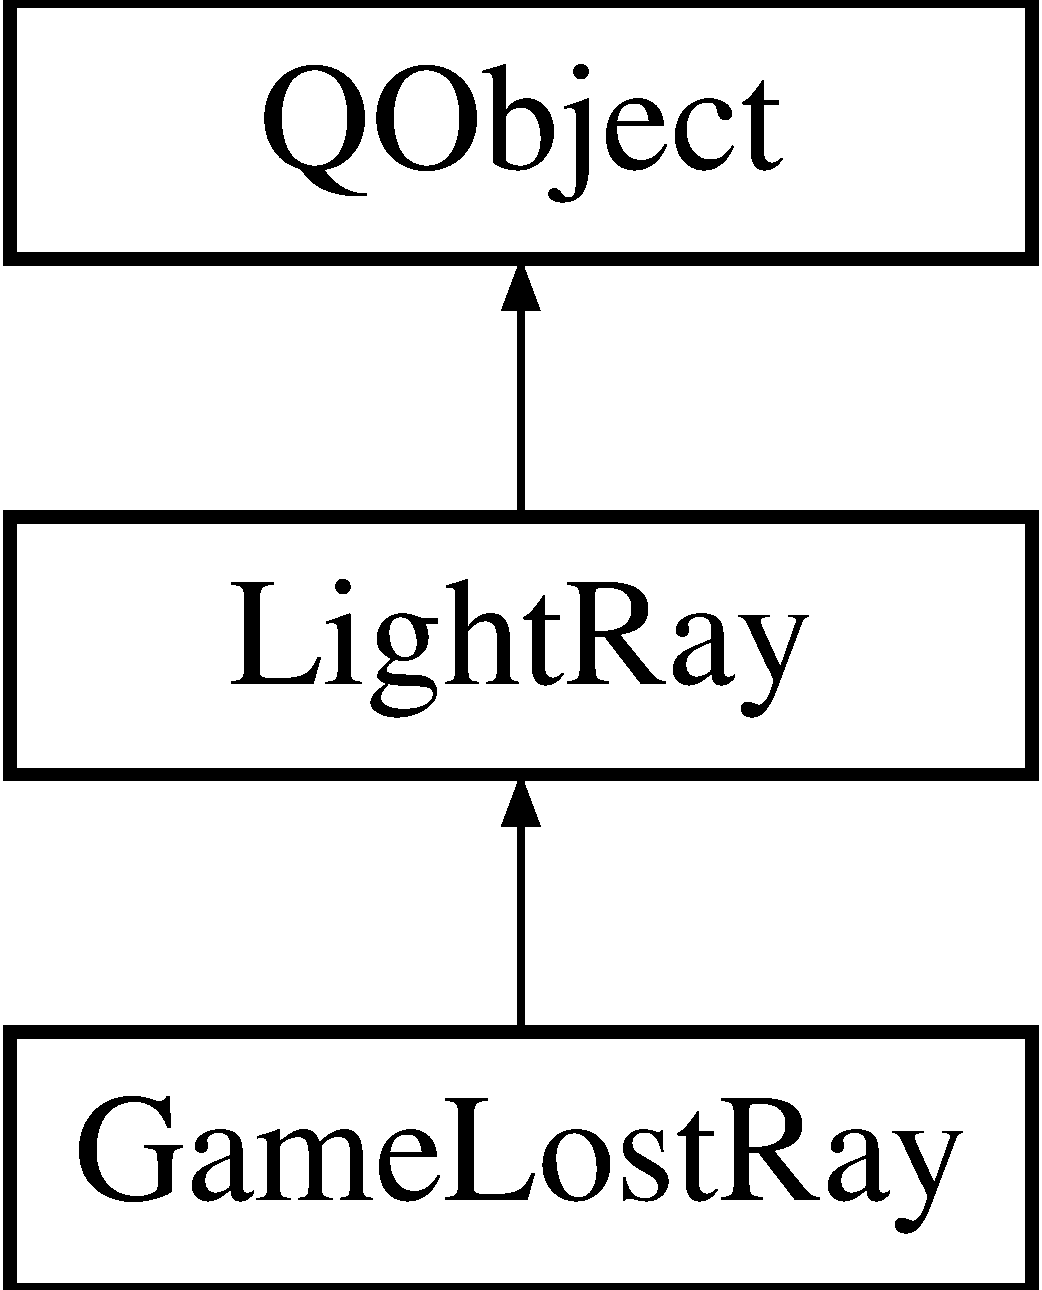
\includegraphics[height=3.000000cm]{class_light_ray}
\end{center}
\end{figure}
\subsection*{Public Slots}
\begin{DoxyCompactItemize}
\item 
const Q\+Vector3\+D \& \hyperlink{class_light_ray_a70d3d18bbecdf54dc399df5112ca024a}{start\+Position} () const 
\item 
void \hyperlink{class_light_ray_a1db98f630b5a18bb297936fc5c8f25fb}{set\+Start\+Position} (const Q\+Vector3\+D \&position)
\item 
const Q\+Vector3\+D \& \hyperlink{class_light_ray_a13026c9fc18cf7fc2d53832223172f13}{end\+Position} () const 
\item 
void \hyperlink{class_light_ray_a5b9d55f5a6bed4b610f1bc294905dd64}{set\+End\+Position} (const Q\+Vector3\+D \&position)
\item 
const Q\+Vector3\+D \& \hyperlink{class_light_ray_af2c247c9b2cc33b4b18ead8e1b12c697}{direction} () const 
\item 
const Q\+Vector3\+D \& \hyperlink{class_light_ray_a1a0dfa514a6c350b78e20903d2fde5c4}{normalized\+Direction} () const 
\item 
const Q\+Vector3\+D \& \hyperlink{class_light_ray_ae816ba62186298d8900e4617034d1d66}{color} () const 
\item 
void \hyperlink{class_light_ray_a607addd328ae2b935d21e093ae15bcd4}{set\+Color} (const Q\+Vector3\+D \&color)
\item 
\hyperlink{class_player}{Player} $\ast$ \hyperlink{class_light_ray_ab2e0d1d08c23a451b83907d61af4297a}{player} () const 
\item 
void \hyperlink{class_light_ray_a3720775f0e8d6c5a8041fd6a7b371dad}{set\+Player} (\hyperlink{class_player}{Player} $\ast$attached\+Player)
\item 
\hyperlink{class_scene}{Scene} $\ast$ \hyperlink{class_light_ray_a7ad5ff6f8863759c2183c95ba8914dfc}{scene} () const 
\item 
void \hyperlink{class_light_ray_a82577f82a77e84b81bd1b722a00bde54}{set\+Scene} (\hyperlink{class_scene}{Scene} $\ast$owning\+Scene)
\item 
bool \hyperlink{class_light_ray_a86e10593e7c2e3a4bbbbf817dd774c27}{is\+Static} () const 
\item 
void \hyperlink{class_light_ray_a6694333616a4d172f1c1bcb4ccbe1587}{set\+Static} ()
\item 
\hyperlink{class_light_ray}{Light\+Ray} $\ast$ \hyperlink{class_light_ray_ad7a12f31f9f84adc155211009a677d77}{selected\+Successor} ()
\begin{DoxyCompactList}\small\item\em Returns the ray the player should move on after reaching end of current ray. In case no successors exists they will be calculated using \hyperlink{class_light_ray_a1711b1964da22ce4083740adc2233780}{calculate\+Successors()} \end{DoxyCompactList}\item 
void \hyperlink{class_light_ray_a2644a596af5de9b41f770131b5c2b0eb}{set\+Selected\+Successor} (\hyperlink{class_light_ray}{Light\+Ray} $\ast$successor)
\item 
const \hyperlink{singleton_q_list}{Q\+List}$<$ \hyperlink{class_light_ray}{Light\+Ray} $\ast$ $>$ \& \hyperlink{class_light_ray_a6673a77eb8fcd32dcfde26a1b112d303}{successors} ()
\end{DoxyCompactItemize}
\subsection*{Signals}
\begin{DoxyCompactItemize}
\item 
void \hyperlink{class_light_ray_a4c9bff5b766f6ba5f4a265cd6aa64958}{color\+Changed} ()
\item 
void \hyperlink{class_light_ray_a5be9eb60aae11d0c24e7db4aa1f89b6c}{start\+Position\+Changed} ()
\item 
void \hyperlink{class_light_ray_a146c3e8249de30de6340fffbf0c1a4d6}{end\+Position\+Changed} ()
\item 
void \hyperlink{class_light_ray_a7b14272e752393259f0b645d92113782}{player\+Changed} ()
\item 
void \hyperlink{class_light_ray_aeea833ba9fe0fe8a3810ba002c3dbec4}{scene\+Changed} ()
\end{DoxyCompactItemize}
\subsection*{Public Member Functions}
\begin{DoxyCompactItemize}
\item 
\hyperlink{class_light_ray_a311f25dc81f2acfe6bc9f7379f76e6fe}{Light\+Ray} (Q\+Object $\ast$parent=0)
\item 
virtual \hyperlink{class_light_ray_a1ec27c859b1851ef680f803ae0555f17}{$\sim$\+Light\+Ray} ()
\item 
virtual void \hyperlink{class_light_ray_acf06a71a307433fa5b220baccf809e64}{update} (int time\+Difference)
\begin{DoxyCompactList}\small\item\em Updates our game. The player will be moved. \end{DoxyCompactList}\item 
Q\+Vector3\+D \hyperlink{class_light_ray_ab8723690d8af8cb9b4ba339eff784135}{normalized\+Orthogonal\+Vector} () const 
\begin{DoxyCompactList}\small\item\em Calculates a normalized vector that is orthogonal to direction(). \end{DoxyCompactList}\item 
Q\+Vector3\+D \hyperlink{class_light_ray_afe5d6813717569166a2c2ca29b2bc923}{calculate\+Color} ()
\begin{DoxyCompactList}\small\item\em calculate\+Successor\+Color calculates the successor color based on its normalized direction The color values are approximately in the range between 0.\+1 and 0.\+8 \end{DoxyCompactList}\end{DoxyCompactItemize}
\subsection*{Protected Member Functions}
\begin{DoxyCompactItemize}
\item 
bool \hyperlink{class_light_ray_ad2f26e29e0781597f7bf106396ba2fb7}{is\+Player\+Before\+Collision\+Point} ()
\item 
void \hyperlink{class_light_ray_a1711b1964da22ce4083740adc2233780}{calculate\+Successors} ()
\item 
\hyperlink{class_abstract_gem}{Abstract\+Gem} $\ast$ \hyperlink{class_light_ray_a9db8f3d965dec84c167b6634bee842f4}{colliding\+Gem} () const 
\item 
void \hyperlink{class_light_ray_a87c45492f6508b5c1adf8300babf8eeb}{set\+Colliding\+Gem} (\hyperlink{class_abstract_gem}{Abstract\+Gem} $\ast$gem)
\end{DoxyCompactItemize}
\subsection*{Protected Attributes}
\begin{DoxyCompactItemize}
\item 
\hyperlink{class_abstract_gem}{Abstract\+Gem} $\ast$ \hyperlink{class_light_ray_ac11396a5ac4a0899ca4bad5d88300fdd}{m\+\_\+colliding\+Gem}
\item 
\hyperlink{class_light_ray_data}{Light\+Ray\+Data} $\ast$ \hyperlink{class_light_ray_acba0c9beeba8ea2863a022910d4ffc34}{m\+\_\+data}
\item 
\hyperlink{singleton_q_list}{Q\+List}$<$ \hyperlink{class_light_ray}{Light\+Ray} $\ast$ $>$ $\ast$ \hyperlink{class_light_ray_a669e04446c77fc44bee41146c1883356}{m\+\_\+successors}
\item 
\hyperlink{class_light_ray}{Light\+Ray} $\ast$ \hyperlink{class_light_ray_a9e430528b861007696716fbd054c9de3}{m\+\_\+selected\+Successor}
\item 
bool \hyperlink{class_light_ray_af44c254c7782710304489afdabd5303a}{m\+\_\+is\+Static}
\item 
\hyperlink{class_player}{Player} $\ast$ \hyperlink{class_light_ray_a55cf457d13b240178933f0a73d6f7b2b}{m\+\_\+player}
\item 
\hyperlink{class_scene}{Scene} $\ast$ \hyperlink{class_light_ray_a9f99d6386ed92c979889f38b5348d628}{m\+\_\+scene}
\end{DoxyCompactItemize}


\subsection{Detailed Description}
The \hyperlink{class_light_ray}{Light\+Ray} class describes the lightrays sent into \hyperlink{class_scene}{Scene}.  Because Light\+Rays are sent into \hyperlink{class_scene}{Scene} right after creation, they are more lines but rays. Rays are organized as a tree, a ray owns all of its \hyperlink{class_light_ray_a6673a77eb8fcd32dcfde26a1b112d303}{successors()}. Most of the game logic is still done within \hyperlink{class_light_ray_acf06a71a307433fa5b220baccf809e64}{Light\+Ray\+::update()}. 

\subsection{Constructor \& Destructor Documentation}
\hypertarget{class_light_ray_a311f25dc81f2acfe6bc9f7379f76e6fe}{\index{Light\+Ray@{Light\+Ray}!Light\+Ray@{Light\+Ray}}
\index{Light\+Ray@{Light\+Ray}!Light\+Ray@{Light\+Ray}}
\subsubsection[{Light\+Ray}]{\setlength{\rightskip}{0pt plus 5cm}Light\+Ray\+::\+Light\+Ray (
\begin{DoxyParamCaption}
\item[{Q\+Object $\ast$}]{parent = {\ttfamily 0}}
\end{DoxyParamCaption}
)\hspace{0.3cm}{\ttfamily [explicit]}}}\label{class_light_ray_a311f25dc81f2acfe6bc9f7379f76e6fe}
\hypertarget{class_light_ray_a1ec27c859b1851ef680f803ae0555f17}{\index{Light\+Ray@{Light\+Ray}!````~Light\+Ray@{$\sim$\+Light\+Ray}}
\index{````~Light\+Ray@{$\sim$\+Light\+Ray}!Light\+Ray@{Light\+Ray}}
\subsubsection[{$\sim$\+Light\+Ray}]{\setlength{\rightskip}{0pt plus 5cm}Light\+Ray\+::$\sim$\+Light\+Ray (
\begin{DoxyParamCaption}
{}
\end{DoxyParamCaption}
)\hspace{0.3cm}{\ttfamily [virtual]}}}\label{class_light_ray_a1ec27c859b1851ef680f803ae0555f17}


\subsection{Member Function Documentation}
\hypertarget{class_light_ray_afe5d6813717569166a2c2ca29b2bc923}{\index{Light\+Ray@{Light\+Ray}!calculate\+Color@{calculate\+Color}}
\index{calculate\+Color@{calculate\+Color}!Light\+Ray@{Light\+Ray}}
\subsubsection[{calculate\+Color}]{\setlength{\rightskip}{0pt plus 5cm}Q\+Vector3\+D Light\+Ray\+::calculate\+Color (
\begin{DoxyParamCaption}
{}
\end{DoxyParamCaption}
)}}\label{class_light_ray_afe5d6813717569166a2c2ca29b2bc923}


calculate\+Successor\+Color calculates the successor color based on its normalized direction The color values are approximately in the range between 0.\+1 and 0.\+8 

\begin{DoxyReturn}{Returns}
The calculated color 
\end{DoxyReturn}
\hypertarget{class_light_ray_a1711b1964da22ce4083740adc2233780}{\index{Light\+Ray@{Light\+Ray}!calculate\+Successors@{calculate\+Successors}}
\index{calculate\+Successors@{calculate\+Successors}!Light\+Ray@{Light\+Ray}}
\subsubsection[{calculate\+Successors}]{\setlength{\rightskip}{0pt plus 5cm}void Light\+Ray\+::calculate\+Successors (
\begin{DoxyParamCaption}
{}
\end{DoxyParamCaption}
)\hspace{0.3cm}{\ttfamily [protected]}}}\label{class_light_ray_a1711b1964da22ce4083740adc2233780}
\hypertarget{class_light_ray_a9db8f3d965dec84c167b6634bee842f4}{\index{Light\+Ray@{Light\+Ray}!colliding\+Gem@{colliding\+Gem}}
\index{colliding\+Gem@{colliding\+Gem}!Light\+Ray@{Light\+Ray}}
\subsubsection[{colliding\+Gem}]{\setlength{\rightskip}{0pt plus 5cm}{\bf Abstract\+Gem} $\ast$ Light\+Ray\+::colliding\+Gem (
\begin{DoxyParamCaption}
{}
\end{DoxyParamCaption}
) const\hspace{0.3cm}{\ttfamily [protected]}}}\label{class_light_ray_a9db8f3d965dec84c167b6634bee842f4}
\hypertarget{class_light_ray_ae816ba62186298d8900e4617034d1d66}{\index{Light\+Ray@{Light\+Ray}!color@{color}}
\index{color@{color}!Light\+Ray@{Light\+Ray}}
\subsubsection[{color}]{\setlength{\rightskip}{0pt plus 5cm}const Q\+Vector3\+D\& Light\+Ray\+::color (
\begin{DoxyParamCaption}
{}
\end{DoxyParamCaption}
) const\hspace{0.3cm}{\ttfamily [slot]}}}\label{class_light_ray_ae816ba62186298d8900e4617034d1d66}
\hypertarget{class_light_ray_a4c9bff5b766f6ba5f4a265cd6aa64958}{\index{Light\+Ray@{Light\+Ray}!color\+Changed@{color\+Changed}}
\index{color\+Changed@{color\+Changed}!Light\+Ray@{Light\+Ray}}
\subsubsection[{color\+Changed}]{\setlength{\rightskip}{0pt plus 5cm}void Light\+Ray\+::color\+Changed (
\begin{DoxyParamCaption}
{}
\end{DoxyParamCaption}
)\hspace{0.3cm}{\ttfamily [signal]}}}\label{class_light_ray_a4c9bff5b766f6ba5f4a265cd6aa64958}
\hypertarget{class_light_ray_af2c247c9b2cc33b4b18ead8e1b12c697}{\index{Light\+Ray@{Light\+Ray}!direction@{direction}}
\index{direction@{direction}!Light\+Ray@{Light\+Ray}}
\subsubsection[{direction}]{\setlength{\rightskip}{0pt plus 5cm}const Q\+Vector3\+D\& Light\+Ray\+::direction (
\begin{DoxyParamCaption}
{}
\end{DoxyParamCaption}
) const\hspace{0.3cm}{\ttfamily [slot]}}}\label{class_light_ray_af2c247c9b2cc33b4b18ead8e1b12c697}
\hypertarget{class_light_ray_a13026c9fc18cf7fc2d53832223172f13}{\index{Light\+Ray@{Light\+Ray}!end\+Position@{end\+Position}}
\index{end\+Position@{end\+Position}!Light\+Ray@{Light\+Ray}}
\subsubsection[{end\+Position}]{\setlength{\rightskip}{0pt plus 5cm}const Q\+Vector3\+D\& Light\+Ray\+::end\+Position (
\begin{DoxyParamCaption}
{}
\end{DoxyParamCaption}
) const\hspace{0.3cm}{\ttfamily [slot]}}}\label{class_light_ray_a13026c9fc18cf7fc2d53832223172f13}
\hypertarget{class_light_ray_a146c3e8249de30de6340fffbf0c1a4d6}{\index{Light\+Ray@{Light\+Ray}!end\+Position\+Changed@{end\+Position\+Changed}}
\index{end\+Position\+Changed@{end\+Position\+Changed}!Light\+Ray@{Light\+Ray}}
\subsubsection[{end\+Position\+Changed}]{\setlength{\rightskip}{0pt plus 5cm}void Light\+Ray\+::end\+Position\+Changed (
\begin{DoxyParamCaption}
{}
\end{DoxyParamCaption}
)\hspace{0.3cm}{\ttfamily [signal]}}}\label{class_light_ray_a146c3e8249de30de6340fffbf0c1a4d6}
\hypertarget{class_light_ray_ad2f26e29e0781597f7bf106396ba2fb7}{\index{Light\+Ray@{Light\+Ray}!is\+Player\+Before\+Collision\+Point@{is\+Player\+Before\+Collision\+Point}}
\index{is\+Player\+Before\+Collision\+Point@{is\+Player\+Before\+Collision\+Point}!Light\+Ray@{Light\+Ray}}
\subsubsection[{is\+Player\+Before\+Collision\+Point}]{\setlength{\rightskip}{0pt plus 5cm}bool Light\+Ray\+::is\+Player\+Before\+Collision\+Point (
\begin{DoxyParamCaption}
{}
\end{DoxyParamCaption}
)\hspace{0.3cm}{\ttfamily [protected]}}}\label{class_light_ray_ad2f26e29e0781597f7bf106396ba2fb7}
\hypertarget{class_light_ray_a86e10593e7c2e3a4bbbbf817dd774c27}{\index{Light\+Ray@{Light\+Ray}!is\+Static@{is\+Static}}
\index{is\+Static@{is\+Static}!Light\+Ray@{Light\+Ray}}
\subsubsection[{is\+Static}]{\setlength{\rightskip}{0pt plus 5cm}bool Light\+Ray\+::is\+Static (
\begin{DoxyParamCaption}
{}
\end{DoxyParamCaption}
) const\hspace{0.3cm}{\ttfamily [slot]}}}\label{class_light_ray_a86e10593e7c2e3a4bbbbf817dd774c27}
\hypertarget{class_light_ray_a1a0dfa514a6c350b78e20903d2fde5c4}{\index{Light\+Ray@{Light\+Ray}!normalized\+Direction@{normalized\+Direction}}
\index{normalized\+Direction@{normalized\+Direction}!Light\+Ray@{Light\+Ray}}
\subsubsection[{normalized\+Direction}]{\setlength{\rightskip}{0pt plus 5cm}const Q\+Vector3\+D\& Light\+Ray\+::normalized\+Direction (
\begin{DoxyParamCaption}
{}
\end{DoxyParamCaption}
) const\hspace{0.3cm}{\ttfamily [slot]}}}\label{class_light_ray_a1a0dfa514a6c350b78e20903d2fde5c4}
\hypertarget{class_light_ray_ab8723690d8af8cb9b4ba339eff784135}{\index{Light\+Ray@{Light\+Ray}!normalized\+Orthogonal\+Vector@{normalized\+Orthogonal\+Vector}}
\index{normalized\+Orthogonal\+Vector@{normalized\+Orthogonal\+Vector}!Light\+Ray@{Light\+Ray}}
\subsubsection[{normalized\+Orthogonal\+Vector}]{\setlength{\rightskip}{0pt plus 5cm}Q\+Vector3\+D Light\+Ray\+::normalized\+Orthogonal\+Vector (
\begin{DoxyParamCaption}
{}
\end{DoxyParamCaption}
) const}}\label{class_light_ray_ab8723690d8af8cb9b4ba339eff784135}


Calculates a normalized vector that is orthogonal to direction(). 

\begin{DoxyReturn}{Returns}

\end{DoxyReturn}
\hypertarget{class_light_ray_ab2e0d1d08c23a451b83907d61af4297a}{\index{Light\+Ray@{Light\+Ray}!player@{player}}
\index{player@{player}!Light\+Ray@{Light\+Ray}}
\subsubsection[{player}]{\setlength{\rightskip}{0pt plus 5cm}{\bf Player}$\ast$ Light\+Ray\+::player (
\begin{DoxyParamCaption}
{}
\end{DoxyParamCaption}
) const\hspace{0.3cm}{\ttfamily [slot]}}}\label{class_light_ray_ab2e0d1d08c23a451b83907d61af4297a}
\hypertarget{class_light_ray_a7b14272e752393259f0b645d92113782}{\index{Light\+Ray@{Light\+Ray}!player\+Changed@{player\+Changed}}
\index{player\+Changed@{player\+Changed}!Light\+Ray@{Light\+Ray}}
\subsubsection[{player\+Changed}]{\setlength{\rightskip}{0pt plus 5cm}void Light\+Ray\+::player\+Changed (
\begin{DoxyParamCaption}
{}
\end{DoxyParamCaption}
)\hspace{0.3cm}{\ttfamily [signal]}}}\label{class_light_ray_a7b14272e752393259f0b645d92113782}
\hypertarget{class_light_ray_a7ad5ff6f8863759c2183c95ba8914dfc}{\index{Light\+Ray@{Light\+Ray}!scene@{scene}}
\index{scene@{scene}!Light\+Ray@{Light\+Ray}}
\subsubsection[{scene}]{\setlength{\rightskip}{0pt plus 5cm}{\bf Scene}$\ast$ Light\+Ray\+::scene (
\begin{DoxyParamCaption}
{}
\end{DoxyParamCaption}
) const\hspace{0.3cm}{\ttfamily [slot]}}}\label{class_light_ray_a7ad5ff6f8863759c2183c95ba8914dfc}
\hypertarget{class_light_ray_aeea833ba9fe0fe8a3810ba002c3dbec4}{\index{Light\+Ray@{Light\+Ray}!scene\+Changed@{scene\+Changed}}
\index{scene\+Changed@{scene\+Changed}!Light\+Ray@{Light\+Ray}}
\subsubsection[{scene\+Changed}]{\setlength{\rightskip}{0pt plus 5cm}void Light\+Ray\+::scene\+Changed (
\begin{DoxyParamCaption}
{}
\end{DoxyParamCaption}
)\hspace{0.3cm}{\ttfamily [signal]}}}\label{class_light_ray_aeea833ba9fe0fe8a3810ba002c3dbec4}
\hypertarget{class_light_ray_ad7a12f31f9f84adc155211009a677d77}{\index{Light\+Ray@{Light\+Ray}!selected\+Successor@{selected\+Successor}}
\index{selected\+Successor@{selected\+Successor}!Light\+Ray@{Light\+Ray}}
\subsubsection[{selected\+Successor}]{\setlength{\rightskip}{0pt plus 5cm}{\bf Light\+Ray} $\ast$ Light\+Ray\+::selected\+Successor (
\begin{DoxyParamCaption}
{}
\end{DoxyParamCaption}
)\hspace{0.3cm}{\ttfamily [slot]}}}\label{class_light_ray_ad7a12f31f9f84adc155211009a677d77}


Returns the ray the player should move on after reaching end of current ray. In case no successors exists they will be calculated using \hyperlink{class_light_ray_a1711b1964da22ce4083740adc2233780}{calculate\+Successors()} 

\begin{DoxyReturn}{Returns}

\end{DoxyReturn}
\hypertarget{class_light_ray_a87c45492f6508b5c1adf8300babf8eeb}{\index{Light\+Ray@{Light\+Ray}!set\+Colliding\+Gem@{set\+Colliding\+Gem}}
\index{set\+Colliding\+Gem@{set\+Colliding\+Gem}!Light\+Ray@{Light\+Ray}}
\subsubsection[{set\+Colliding\+Gem}]{\setlength{\rightskip}{0pt plus 5cm}void Light\+Ray\+::set\+Colliding\+Gem (
\begin{DoxyParamCaption}
\item[{{\bf Abstract\+Gem} $\ast$}]{gem}
\end{DoxyParamCaption}
)\hspace{0.3cm}{\ttfamily [protected]}}}\label{class_light_ray_a87c45492f6508b5c1adf8300babf8eeb}
\hypertarget{class_light_ray_a607addd328ae2b935d21e093ae15bcd4}{\index{Light\+Ray@{Light\+Ray}!set\+Color@{set\+Color}}
\index{set\+Color@{set\+Color}!Light\+Ray@{Light\+Ray}}
\subsubsection[{set\+Color}]{\setlength{\rightskip}{0pt plus 5cm}void Light\+Ray\+::set\+Color (
\begin{DoxyParamCaption}
\item[{const Q\+Vector3\+D \&}]{color}
\end{DoxyParamCaption}
)\hspace{0.3cm}{\ttfamily [slot]}}}\label{class_light_ray_a607addd328ae2b935d21e093ae15bcd4}
\hypertarget{class_light_ray_a5b9d55f5a6bed4b610f1bc294905dd64}{\index{Light\+Ray@{Light\+Ray}!set\+End\+Position@{set\+End\+Position}}
\index{set\+End\+Position@{set\+End\+Position}!Light\+Ray@{Light\+Ray}}
\subsubsection[{set\+End\+Position}]{\setlength{\rightskip}{0pt plus 5cm}void Light\+Ray\+::set\+End\+Position (
\begin{DoxyParamCaption}
\item[{const Q\+Vector3\+D \&}]{position}
\end{DoxyParamCaption}
)\hspace{0.3cm}{\ttfamily [slot]}}}\label{class_light_ray_a5b9d55f5a6bed4b610f1bc294905dd64}
\hypertarget{class_light_ray_a3720775f0e8d6c5a8041fd6a7b371dad}{\index{Light\+Ray@{Light\+Ray}!set\+Player@{set\+Player}}
\index{set\+Player@{set\+Player}!Light\+Ray@{Light\+Ray}}
\subsubsection[{set\+Player}]{\setlength{\rightskip}{0pt plus 5cm}void Light\+Ray\+::set\+Player (
\begin{DoxyParamCaption}
\item[{{\bf Player} $\ast$}]{attached\+Player}
\end{DoxyParamCaption}
)\hspace{0.3cm}{\ttfamily [slot]}}}\label{class_light_ray_a3720775f0e8d6c5a8041fd6a7b371dad}
\hypertarget{class_light_ray_a82577f82a77e84b81bd1b722a00bde54}{\index{Light\+Ray@{Light\+Ray}!set\+Scene@{set\+Scene}}
\index{set\+Scene@{set\+Scene}!Light\+Ray@{Light\+Ray}}
\subsubsection[{set\+Scene}]{\setlength{\rightskip}{0pt plus 5cm}void Light\+Ray\+::set\+Scene (
\begin{DoxyParamCaption}
\item[{{\bf Scene} $\ast$}]{owning\+Scene}
\end{DoxyParamCaption}
)\hspace{0.3cm}{\ttfamily [slot]}}}\label{class_light_ray_a82577f82a77e84b81bd1b722a00bde54}
\hypertarget{class_light_ray_a2644a596af5de9b41f770131b5c2b0eb}{\index{Light\+Ray@{Light\+Ray}!set\+Selected\+Successor@{set\+Selected\+Successor}}
\index{set\+Selected\+Successor@{set\+Selected\+Successor}!Light\+Ray@{Light\+Ray}}
\subsubsection[{set\+Selected\+Successor}]{\setlength{\rightskip}{0pt plus 5cm}void Light\+Ray\+::set\+Selected\+Successor (
\begin{DoxyParamCaption}
\item[{{\bf Light\+Ray} $\ast$}]{successor}
\end{DoxyParamCaption}
)\hspace{0.3cm}{\ttfamily [slot]}}}\label{class_light_ray_a2644a596af5de9b41f770131b5c2b0eb}
\hypertarget{class_light_ray_a1db98f630b5a18bb297936fc5c8f25fb}{\index{Light\+Ray@{Light\+Ray}!set\+Start\+Position@{set\+Start\+Position}}
\index{set\+Start\+Position@{set\+Start\+Position}!Light\+Ray@{Light\+Ray}}
\subsubsection[{set\+Start\+Position}]{\setlength{\rightskip}{0pt plus 5cm}void Light\+Ray\+::set\+Start\+Position (
\begin{DoxyParamCaption}
\item[{const Q\+Vector3\+D \&}]{position}
\end{DoxyParamCaption}
)\hspace{0.3cm}{\ttfamily [slot]}}}\label{class_light_ray_a1db98f630b5a18bb297936fc5c8f25fb}
\hypertarget{class_light_ray_a6694333616a4d172f1c1bcb4ccbe1587}{\index{Light\+Ray@{Light\+Ray}!set\+Static@{set\+Static}}
\index{set\+Static@{set\+Static}!Light\+Ray@{Light\+Ray}}
\subsubsection[{set\+Static}]{\setlength{\rightskip}{0pt plus 5cm}void Light\+Ray\+::set\+Static (
\begin{DoxyParamCaption}
{}
\end{DoxyParamCaption}
)\hspace{0.3cm}{\ttfamily [slot]}}}\label{class_light_ray_a6694333616a4d172f1c1bcb4ccbe1587}
\hypertarget{class_light_ray_a70d3d18bbecdf54dc399df5112ca024a}{\index{Light\+Ray@{Light\+Ray}!start\+Position@{start\+Position}}
\index{start\+Position@{start\+Position}!Light\+Ray@{Light\+Ray}}
\subsubsection[{start\+Position}]{\setlength{\rightskip}{0pt plus 5cm}const Q\+Vector3\+D\& Light\+Ray\+::start\+Position (
\begin{DoxyParamCaption}
{}
\end{DoxyParamCaption}
) const\hspace{0.3cm}{\ttfamily [slot]}}}\label{class_light_ray_a70d3d18bbecdf54dc399df5112ca024a}
\hypertarget{class_light_ray_a5be9eb60aae11d0c24e7db4aa1f89b6c}{\index{Light\+Ray@{Light\+Ray}!start\+Position\+Changed@{start\+Position\+Changed}}
\index{start\+Position\+Changed@{start\+Position\+Changed}!Light\+Ray@{Light\+Ray}}
\subsubsection[{start\+Position\+Changed}]{\setlength{\rightskip}{0pt plus 5cm}void Light\+Ray\+::start\+Position\+Changed (
\begin{DoxyParamCaption}
{}
\end{DoxyParamCaption}
)\hspace{0.3cm}{\ttfamily [signal]}}}\label{class_light_ray_a5be9eb60aae11d0c24e7db4aa1f89b6c}
\hypertarget{class_light_ray_a6673a77eb8fcd32dcfde26a1b112d303}{\index{Light\+Ray@{Light\+Ray}!successors@{successors}}
\index{successors@{successors}!Light\+Ray@{Light\+Ray}}
\subsubsection[{successors}]{\setlength{\rightskip}{0pt plus 5cm}const {\bf Q\+List}$<$ {\bf Light\+Ray} $\ast$ $>$ \& Light\+Ray\+::successors (
\begin{DoxyParamCaption}
{}
\end{DoxyParamCaption}
)\hspace{0.3cm}{\ttfamily [slot]}}}\label{class_light_ray_a6673a77eb8fcd32dcfde26a1b112d303}
\hypertarget{class_light_ray_acf06a71a307433fa5b220baccf809e64}{\index{Light\+Ray@{Light\+Ray}!update@{update}}
\index{update@{update}!Light\+Ray@{Light\+Ray}}
\subsubsection[{update}]{\setlength{\rightskip}{0pt plus 5cm}void Light\+Ray\+::update (
\begin{DoxyParamCaption}
\item[{int}]{time\+Difference}
\end{DoxyParamCaption}
)\hspace{0.3cm}{\ttfamily [virtual]}}}\label{class_light_ray_acf06a71a307433fa5b220baccf809e64}


Updates our game. The player will be moved. 


\begin{DoxyParams}{Parameters}
{\em time\+Difference} & Time since last update in milliseconds. \\
\hline
\end{DoxyParams}


Reimplemented in \hyperlink{class_game_lost_ray_a417d814372891fe7595a7e745b7a9f0f}{Game\+Lost\+Ray}.



\subsection{Member Data Documentation}
\hypertarget{class_light_ray_ac11396a5ac4a0899ca4bad5d88300fdd}{\index{Light\+Ray@{Light\+Ray}!m\+\_\+colliding\+Gem@{m\+\_\+colliding\+Gem}}
\index{m\+\_\+colliding\+Gem@{m\+\_\+colliding\+Gem}!Light\+Ray@{Light\+Ray}}
\subsubsection[{m\+\_\+colliding\+Gem}]{\setlength{\rightskip}{0pt plus 5cm}{\bf Abstract\+Gem}$\ast$ Light\+Ray\+::m\+\_\+colliding\+Gem\hspace{0.3cm}{\ttfamily [protected]}}}\label{class_light_ray_ac11396a5ac4a0899ca4bad5d88300fdd}
\hypertarget{class_light_ray_acba0c9beeba8ea2863a022910d4ffc34}{\index{Light\+Ray@{Light\+Ray}!m\+\_\+data@{m\+\_\+data}}
\index{m\+\_\+data@{m\+\_\+data}!Light\+Ray@{Light\+Ray}}
\subsubsection[{m\+\_\+data}]{\setlength{\rightskip}{0pt plus 5cm}{\bf Light\+Ray\+Data}$\ast$ Light\+Ray\+::m\+\_\+data\hspace{0.3cm}{\ttfamily [protected]}}}\label{class_light_ray_acba0c9beeba8ea2863a022910d4ffc34}
\hypertarget{class_light_ray_af44c254c7782710304489afdabd5303a}{\index{Light\+Ray@{Light\+Ray}!m\+\_\+is\+Static@{m\+\_\+is\+Static}}
\index{m\+\_\+is\+Static@{m\+\_\+is\+Static}!Light\+Ray@{Light\+Ray}}
\subsubsection[{m\+\_\+is\+Static}]{\setlength{\rightskip}{0pt plus 5cm}bool Light\+Ray\+::m\+\_\+is\+Static\hspace{0.3cm}{\ttfamily [protected]}}}\label{class_light_ray_af44c254c7782710304489afdabd5303a}
\hypertarget{class_light_ray_a55cf457d13b240178933f0a73d6f7b2b}{\index{Light\+Ray@{Light\+Ray}!m\+\_\+player@{m\+\_\+player}}
\index{m\+\_\+player@{m\+\_\+player}!Light\+Ray@{Light\+Ray}}
\subsubsection[{m\+\_\+player}]{\setlength{\rightskip}{0pt plus 5cm}{\bf Player}$\ast$ Light\+Ray\+::m\+\_\+player\hspace{0.3cm}{\ttfamily [protected]}}}\label{class_light_ray_a55cf457d13b240178933f0a73d6f7b2b}
\hypertarget{class_light_ray_a9f99d6386ed92c979889f38b5348d628}{\index{Light\+Ray@{Light\+Ray}!m\+\_\+scene@{m\+\_\+scene}}
\index{m\+\_\+scene@{m\+\_\+scene}!Light\+Ray@{Light\+Ray}}
\subsubsection[{m\+\_\+scene}]{\setlength{\rightskip}{0pt plus 5cm}{\bf Scene}$\ast$ Light\+Ray\+::m\+\_\+scene\hspace{0.3cm}{\ttfamily [protected]}}}\label{class_light_ray_a9f99d6386ed92c979889f38b5348d628}
\hypertarget{class_light_ray_a9e430528b861007696716fbd054c9de3}{\index{Light\+Ray@{Light\+Ray}!m\+\_\+selected\+Successor@{m\+\_\+selected\+Successor}}
\index{m\+\_\+selected\+Successor@{m\+\_\+selected\+Successor}!Light\+Ray@{Light\+Ray}}
\subsubsection[{m\+\_\+selected\+Successor}]{\setlength{\rightskip}{0pt plus 5cm}{\bf Light\+Ray}$\ast$ Light\+Ray\+::m\+\_\+selected\+Successor\hspace{0.3cm}{\ttfamily [protected]}}}\label{class_light_ray_a9e430528b861007696716fbd054c9de3}
\hypertarget{class_light_ray_a669e04446c77fc44bee41146c1883356}{\index{Light\+Ray@{Light\+Ray}!m\+\_\+successors@{m\+\_\+successors}}
\index{m\+\_\+successors@{m\+\_\+successors}!Light\+Ray@{Light\+Ray}}
\subsubsection[{m\+\_\+successors}]{\setlength{\rightskip}{0pt plus 5cm}{\bf Q\+List}$<${\bf Light\+Ray} $\ast$$>$$\ast$ Light\+Ray\+::m\+\_\+successors\hspace{0.3cm}{\ttfamily [protected]}}}\label{class_light_ray_a669e04446c77fc44bee41146c1883356}


The documentation for this class was generated from the following files\+:\begin{DoxyCompactItemize}
\item 
\hyperlink{lightray_8h}{lightray.\+h}\item 
\hyperlink{lightray_8cpp}{lightray.\+cpp}\end{DoxyCompactItemize}

\hypertarget{class_light_ray_data}{}\section{Light\+Ray\+Data Class Reference}
\label{class_light_ray_data}\index{Light\+Ray\+Data@{Light\+Ray\+Data}}


The \hyperlink{class_light_ray_data}{Light\+Ray\+Data} class stores data of a \hyperlink{class_light_ray}{Light\+Ray}. The \hyperlink{class_light_ray_data}{Light\+Ray\+Data} doesn\textquotesingle{}t inherit from Q\+Object, so it can be stored in Qt-\/\+Containers (currently only those require == or q\+Hash) by Value. Also the data can be copied easily.  




{\ttfamily \#include $<$lightraydata.\+h$>$}

\subsection*{Public Member Functions}
\begin{DoxyCompactItemize}
\item 
\hyperlink{class_light_ray_data_ac0cb11da1651f8ff7b8ed9d785b68a27}{Light\+Ray\+Data} ()
\item 
\hyperlink{class_light_ray_data_a50350aa163fd7c1a54f97cefafd2d2f7}{Light\+Ray\+Data} (const \hyperlink{class_light_ray}{Light\+Ray} \&light\+Ray)
\item 
\hyperlink{class_light_ray_data_a9344f139cafb257f61f4d800fbecd905}{Light\+Ray\+Data} (const \hyperlink{class_light_ray_data}{Light\+Ray\+Data} \&light\+Ray)
\item 
\hyperlink{class_light_ray_data_a6cd92465c9ba1da296d30a32487a6ac0}{$\sim$\+Light\+Ray\+Data} ()
\item 
Q\+Vector3\+D \hyperlink{class_light_ray_data_acada2319ae380a11a405817cd9cd3d65}{normalized\+Orthogonal\+Vector} () const 
\begin{DoxyCompactList}\small\item\em Calculates a normalized vector, that is orthogonal to \hyperlink{class_light_ray_data_aaecf9f1d378eebf6d577eaa588930a4f}{direction()}. \end{DoxyCompactList}\item 
const Q\+Vector3\+D \& \hyperlink{class_light_ray_data_a64a5b7f8d4c3af9cc3e8c1a6c6ea8c57}{color} () const 
\item 
void \hyperlink{class_light_ray_data_ad8fead207765a43bb1167e2ce95e85a4}{set\+Color} (const Q\+Vector3\+D \&\hyperlink{class_light_ray_data_a64a5b7f8d4c3af9cc3e8c1a6c6ea8c57}{color})
\item 
const Q\+Vector3\+D \& \hyperlink{class_light_ray_data_af040092e873e42d0d31f803452fc648e}{start\+Position} () const 
\item 
void \hyperlink{class_light_ray_data_a464a868047052152f375cb45ac476eb2}{set\+Start\+Position} (const Q\+Vector3\+D \&position)
\item 
const Q\+Vector3\+D \& \hyperlink{class_light_ray_data_ab47d397dcffe8a2c8da0cf4d8bbbd2bc}{end\+Position} () const 
\item 
void \hyperlink{class_light_ray_data_ad7ec7b96408f0fb7f603687c54804d3b}{set\+End\+Position} (const Q\+Vector3\+D \&position)
\item 
const Q\+Vector3\+D \& \hyperlink{class_light_ray_data_aaecf9f1d378eebf6d577eaa588930a4f}{direction} () const 
\item 
const Q\+Vector3\+D \& \hyperlink{class_light_ray_data_a791bbf3c85d32004d0d7d155cd248a43}{normalized\+Direction} () const 
\item 
\hyperlink{class_light_ray_data}{Light\+Ray\+Data} \& \hyperlink{class_light_ray_data_a2dc01f58929829517a90b1fc29f12942}{operator=} (const \hyperlink{class_light_ray_data}{Light\+Ray\+Data} \&light\+Ray)
\end{DoxyCompactItemize}
\subsection*{Protected Attributes}
\begin{DoxyCompactItemize}
\item 
Q\+Vector3\+D $\ast$ \hyperlink{class_light_ray_data_ae6ad9fa7cd9bc9db1837691c603e5eaa}{m\+\_\+color}
\item 
Q\+Vector3\+D $\ast$ \hyperlink{class_light_ray_data_a4a71e8787288d9e243c3c9dd744350ff}{m\+\_\+direction}
\item 
Q\+Vector3\+D $\ast$ \hyperlink{class_light_ray_data_af18cf984ba862735dcde2d77767c4bb2}{m\+\_\+direction\+Normalized}
\item 
Q\+Vector3\+D $\ast$ \hyperlink{class_light_ray_data_ab7228a576b4b1c0843641e3706a6cb35}{m\+\_\+end\+Position}
\item 
Q\+Vector3\+D $\ast$ \hyperlink{class_light_ray_data_a1da577bdf12b630015fca5d89712e479}{m\+\_\+start\+Position}
\end{DoxyCompactItemize}


\subsection{Detailed Description}
The \hyperlink{class_light_ray_data}{Light\+Ray\+Data} class stores data of a \hyperlink{class_light_ray}{Light\+Ray}. The \hyperlink{class_light_ray_data}{Light\+Ray\+Data} doesn\textquotesingle{}t inherit from Q\+Object, so it can be stored in Qt-\/\+Containers (currently only those require == or q\+Hash) by Value. Also the data can be copied easily. 

\subsection{Constructor \& Destructor Documentation}
\hypertarget{class_light_ray_data_ac0cb11da1651f8ff7b8ed9d785b68a27}{}\index{Light\+Ray\+Data@{Light\+Ray\+Data}!Light\+Ray\+Data@{Light\+Ray\+Data}}
\index{Light\+Ray\+Data@{Light\+Ray\+Data}!Light\+Ray\+Data@{Light\+Ray\+Data}}
\subsubsection[{Light\+Ray\+Data}]{\setlength{\rightskip}{0pt plus 5cm}Light\+Ray\+Data\+::\+Light\+Ray\+Data (
\begin{DoxyParamCaption}
{}
\end{DoxyParamCaption}
)}\label{class_light_ray_data_ac0cb11da1651f8ff7b8ed9d785b68a27}
\hypertarget{class_light_ray_data_a50350aa163fd7c1a54f97cefafd2d2f7}{}\index{Light\+Ray\+Data@{Light\+Ray\+Data}!Light\+Ray\+Data@{Light\+Ray\+Data}}
\index{Light\+Ray\+Data@{Light\+Ray\+Data}!Light\+Ray\+Data@{Light\+Ray\+Data}}
\subsubsection[{Light\+Ray\+Data}]{\setlength{\rightskip}{0pt plus 5cm}Light\+Ray\+Data\+::\+Light\+Ray\+Data (
\begin{DoxyParamCaption}
\item[{const {\bf Light\+Ray} \&}]{light\+Ray}
\end{DoxyParamCaption}
)}\label{class_light_ray_data_a50350aa163fd7c1a54f97cefafd2d2f7}
\hypertarget{class_light_ray_data_a9344f139cafb257f61f4d800fbecd905}{}\index{Light\+Ray\+Data@{Light\+Ray\+Data}!Light\+Ray\+Data@{Light\+Ray\+Data}}
\index{Light\+Ray\+Data@{Light\+Ray\+Data}!Light\+Ray\+Data@{Light\+Ray\+Data}}
\subsubsection[{Light\+Ray\+Data}]{\setlength{\rightskip}{0pt plus 5cm}Light\+Ray\+Data\+::\+Light\+Ray\+Data (
\begin{DoxyParamCaption}
\item[{const {\bf Light\+Ray\+Data} \&}]{light\+Ray}
\end{DoxyParamCaption}
)}\label{class_light_ray_data_a9344f139cafb257f61f4d800fbecd905}
\hypertarget{class_light_ray_data_a6cd92465c9ba1da296d30a32487a6ac0}{}\index{Light\+Ray\+Data@{Light\+Ray\+Data}!````~Light\+Ray\+Data@{$\sim$\+Light\+Ray\+Data}}
\index{````~Light\+Ray\+Data@{$\sim$\+Light\+Ray\+Data}!Light\+Ray\+Data@{Light\+Ray\+Data}}
\subsubsection[{$\sim$\+Light\+Ray\+Data}]{\setlength{\rightskip}{0pt plus 5cm}Light\+Ray\+Data\+::$\sim$\+Light\+Ray\+Data (
\begin{DoxyParamCaption}
{}
\end{DoxyParamCaption}
)}\label{class_light_ray_data_a6cd92465c9ba1da296d30a32487a6ac0}


\subsection{Member Function Documentation}
\hypertarget{class_light_ray_data_a64a5b7f8d4c3af9cc3e8c1a6c6ea8c57}{}\index{Light\+Ray\+Data@{Light\+Ray\+Data}!color@{color}}
\index{color@{color}!Light\+Ray\+Data@{Light\+Ray\+Data}}
\subsubsection[{color}]{\setlength{\rightskip}{0pt plus 5cm}const Q\+Vector3\+D \& Light\+Ray\+Data\+::color (
\begin{DoxyParamCaption}
{}
\end{DoxyParamCaption}
) const}\label{class_light_ray_data_a64a5b7f8d4c3af9cc3e8c1a6c6ea8c57}
\hypertarget{class_light_ray_data_aaecf9f1d378eebf6d577eaa588930a4f}{}\index{Light\+Ray\+Data@{Light\+Ray\+Data}!direction@{direction}}
\index{direction@{direction}!Light\+Ray\+Data@{Light\+Ray\+Data}}
\subsubsection[{direction}]{\setlength{\rightskip}{0pt plus 5cm}const Q\+Vector3\+D \& Light\+Ray\+Data\+::direction (
\begin{DoxyParamCaption}
{}
\end{DoxyParamCaption}
) const}\label{class_light_ray_data_aaecf9f1d378eebf6d577eaa588930a4f}
\hypertarget{class_light_ray_data_ab47d397dcffe8a2c8da0cf4d8bbbd2bc}{}\index{Light\+Ray\+Data@{Light\+Ray\+Data}!end\+Position@{end\+Position}}
\index{end\+Position@{end\+Position}!Light\+Ray\+Data@{Light\+Ray\+Data}}
\subsubsection[{end\+Position}]{\setlength{\rightskip}{0pt plus 5cm}const Q\+Vector3\+D \& Light\+Ray\+Data\+::end\+Position (
\begin{DoxyParamCaption}
{}
\end{DoxyParamCaption}
) const}\label{class_light_ray_data_ab47d397dcffe8a2c8da0cf4d8bbbd2bc}
\hypertarget{class_light_ray_data_a791bbf3c85d32004d0d7d155cd248a43}{}\index{Light\+Ray\+Data@{Light\+Ray\+Data}!normalized\+Direction@{normalized\+Direction}}
\index{normalized\+Direction@{normalized\+Direction}!Light\+Ray\+Data@{Light\+Ray\+Data}}
\subsubsection[{normalized\+Direction}]{\setlength{\rightskip}{0pt plus 5cm}const Q\+Vector3\+D \& Light\+Ray\+Data\+::normalized\+Direction (
\begin{DoxyParamCaption}
{}
\end{DoxyParamCaption}
) const}\label{class_light_ray_data_a791bbf3c85d32004d0d7d155cd248a43}
\hypertarget{class_light_ray_data_acada2319ae380a11a405817cd9cd3d65}{}\index{Light\+Ray\+Data@{Light\+Ray\+Data}!normalized\+Orthogonal\+Vector@{normalized\+Orthogonal\+Vector}}
\index{normalized\+Orthogonal\+Vector@{normalized\+Orthogonal\+Vector}!Light\+Ray\+Data@{Light\+Ray\+Data}}
\subsubsection[{normalized\+Orthogonal\+Vector}]{\setlength{\rightskip}{0pt plus 5cm}Q\+Vector3\+D Light\+Ray\+Data\+::normalized\+Orthogonal\+Vector (
\begin{DoxyParamCaption}
{}
\end{DoxyParamCaption}
) const}\label{class_light_ray_data_acada2319ae380a11a405817cd9cd3d65}


Calculates a normalized vector, that is orthogonal to \hyperlink{class_light_ray_data_aaecf9f1d378eebf6d577eaa588930a4f}{direction()}. 

\begin{DoxyReturn}{Returns}

\end{DoxyReturn}
\hypertarget{class_light_ray_data_a2dc01f58929829517a90b1fc29f12942}{}\index{Light\+Ray\+Data@{Light\+Ray\+Data}!operator=@{operator=}}
\index{operator=@{operator=}!Light\+Ray\+Data@{Light\+Ray\+Data}}
\subsubsection[{operator=}]{\setlength{\rightskip}{0pt plus 5cm}{\bf Light\+Ray\+Data} \& Light\+Ray\+Data\+::operator= (
\begin{DoxyParamCaption}
\item[{const {\bf Light\+Ray\+Data} \&}]{light\+Ray}
\end{DoxyParamCaption}
)}\label{class_light_ray_data_a2dc01f58929829517a90b1fc29f12942}
\hypertarget{class_light_ray_data_ad8fead207765a43bb1167e2ce95e85a4}{}\index{Light\+Ray\+Data@{Light\+Ray\+Data}!set\+Color@{set\+Color}}
\index{set\+Color@{set\+Color}!Light\+Ray\+Data@{Light\+Ray\+Data}}
\subsubsection[{set\+Color}]{\setlength{\rightskip}{0pt plus 5cm}void Light\+Ray\+Data\+::set\+Color (
\begin{DoxyParamCaption}
\item[{const Q\+Vector3\+D \&}]{color}
\end{DoxyParamCaption}
)}\label{class_light_ray_data_ad8fead207765a43bb1167e2ce95e85a4}
\hypertarget{class_light_ray_data_ad7ec7b96408f0fb7f603687c54804d3b}{}\index{Light\+Ray\+Data@{Light\+Ray\+Data}!set\+End\+Position@{set\+End\+Position}}
\index{set\+End\+Position@{set\+End\+Position}!Light\+Ray\+Data@{Light\+Ray\+Data}}
\subsubsection[{set\+End\+Position}]{\setlength{\rightskip}{0pt plus 5cm}void Light\+Ray\+Data\+::set\+End\+Position (
\begin{DoxyParamCaption}
\item[{const Q\+Vector3\+D \&}]{position}
\end{DoxyParamCaption}
)}\label{class_light_ray_data_ad7ec7b96408f0fb7f603687c54804d3b}
\hypertarget{class_light_ray_data_a464a868047052152f375cb45ac476eb2}{}\index{Light\+Ray\+Data@{Light\+Ray\+Data}!set\+Start\+Position@{set\+Start\+Position}}
\index{set\+Start\+Position@{set\+Start\+Position}!Light\+Ray\+Data@{Light\+Ray\+Data}}
\subsubsection[{set\+Start\+Position}]{\setlength{\rightskip}{0pt plus 5cm}void Light\+Ray\+Data\+::set\+Start\+Position (
\begin{DoxyParamCaption}
\item[{const Q\+Vector3\+D \&}]{position}
\end{DoxyParamCaption}
)}\label{class_light_ray_data_a464a868047052152f375cb45ac476eb2}
\hypertarget{class_light_ray_data_af040092e873e42d0d31f803452fc648e}{}\index{Light\+Ray\+Data@{Light\+Ray\+Data}!start\+Position@{start\+Position}}
\index{start\+Position@{start\+Position}!Light\+Ray\+Data@{Light\+Ray\+Data}}
\subsubsection[{start\+Position}]{\setlength{\rightskip}{0pt plus 5cm}const Q\+Vector3\+D \& Light\+Ray\+Data\+::start\+Position (
\begin{DoxyParamCaption}
{}
\end{DoxyParamCaption}
) const}\label{class_light_ray_data_af040092e873e42d0d31f803452fc648e}


\subsection{Member Data Documentation}
\hypertarget{class_light_ray_data_ae6ad9fa7cd9bc9db1837691c603e5eaa}{}\index{Light\+Ray\+Data@{Light\+Ray\+Data}!m\+\_\+color@{m\+\_\+color}}
\index{m\+\_\+color@{m\+\_\+color}!Light\+Ray\+Data@{Light\+Ray\+Data}}
\subsubsection[{m\+\_\+color}]{\setlength{\rightskip}{0pt plus 5cm}Q\+Vector3\+D$\ast$ Light\+Ray\+Data\+::m\+\_\+color\hspace{0.3cm}{\ttfamily [protected]}}\label{class_light_ray_data_ae6ad9fa7cd9bc9db1837691c603e5eaa}
\hypertarget{class_light_ray_data_a4a71e8787288d9e243c3c9dd744350ff}{}\index{Light\+Ray\+Data@{Light\+Ray\+Data}!m\+\_\+direction@{m\+\_\+direction}}
\index{m\+\_\+direction@{m\+\_\+direction}!Light\+Ray\+Data@{Light\+Ray\+Data}}
\subsubsection[{m\+\_\+direction}]{\setlength{\rightskip}{0pt plus 5cm}Q\+Vector3\+D$\ast$ Light\+Ray\+Data\+::m\+\_\+direction\hspace{0.3cm}{\ttfamily [protected]}}\label{class_light_ray_data_a4a71e8787288d9e243c3c9dd744350ff}
\hypertarget{class_light_ray_data_af18cf984ba862735dcde2d77767c4bb2}{}\index{Light\+Ray\+Data@{Light\+Ray\+Data}!m\+\_\+direction\+Normalized@{m\+\_\+direction\+Normalized}}
\index{m\+\_\+direction\+Normalized@{m\+\_\+direction\+Normalized}!Light\+Ray\+Data@{Light\+Ray\+Data}}
\subsubsection[{m\+\_\+direction\+Normalized}]{\setlength{\rightskip}{0pt plus 5cm}Q\+Vector3\+D$\ast$ Light\+Ray\+Data\+::m\+\_\+direction\+Normalized\hspace{0.3cm}{\ttfamily [protected]}}\label{class_light_ray_data_af18cf984ba862735dcde2d77767c4bb2}
\hypertarget{class_light_ray_data_ab7228a576b4b1c0843641e3706a6cb35}{}\index{Light\+Ray\+Data@{Light\+Ray\+Data}!m\+\_\+end\+Position@{m\+\_\+end\+Position}}
\index{m\+\_\+end\+Position@{m\+\_\+end\+Position}!Light\+Ray\+Data@{Light\+Ray\+Data}}
\subsubsection[{m\+\_\+end\+Position}]{\setlength{\rightskip}{0pt plus 5cm}Q\+Vector3\+D$\ast$ Light\+Ray\+Data\+::m\+\_\+end\+Position\hspace{0.3cm}{\ttfamily [protected]}}\label{class_light_ray_data_ab7228a576b4b1c0843641e3706a6cb35}
\hypertarget{class_light_ray_data_a1da577bdf12b630015fca5d89712e479}{}\index{Light\+Ray\+Data@{Light\+Ray\+Data}!m\+\_\+start\+Position@{m\+\_\+start\+Position}}
\index{m\+\_\+start\+Position@{m\+\_\+start\+Position}!Light\+Ray\+Data@{Light\+Ray\+Data}}
\subsubsection[{m\+\_\+start\+Position}]{\setlength{\rightskip}{0pt plus 5cm}Q\+Vector3\+D$\ast$ Light\+Ray\+Data\+::m\+\_\+start\+Position\hspace{0.3cm}{\ttfamily [protected]}}\label{class_light_ray_data_a1da577bdf12b630015fca5d89712e479}


The documentation for this class was generated from the following files\+:\begin{DoxyCompactItemize}
\item 
Game-\/\+Programming-\/\+W\+S2014/gem\+Illuminator/\hyperlink{lightraydata_8h}{lightraydata.\+h}\item 
Game-\/\+Programming-\/\+W\+S2014/gem\+Illuminator/\hyperlink{lightraydata_8cpp}{lightraydata.\+cpp}\end{DoxyCompactItemize}

\hypertarget{class_light_ray_renderer}{}\section{Light\+Ray\+Renderer Class Reference}
\label{class_light_ray_renderer}\index{Light\+Ray\+Renderer@{Light\+Ray\+Renderer}}


The \hyperlink{class_light_ray_renderer}{Light\+Ray\+Renderer} packs Light\+Rays and paint them.  




{\ttfamily \#include $<$lightrayrenderer.\+h$>$}

Inheritance diagram for Light\+Ray\+Renderer\+:\begin{figure}[H]
\begin{center}
\leavevmode
\includegraphics[height=2.000000cm]{class_light_ray_renderer}
\end{center}
\end{figure}
\subsection*{Public Member Functions}
\begin{DoxyCompactItemize}
\item 
\hyperlink{class_light_ray_renderer_a081e83e5e16a36faec002878052aab04}{Light\+Ray\+Renderer} (Q\+Object $\ast$parent=0)
\item 
virtual \hyperlink{class_light_ray_renderer_ac751be83a9d351286b0f89693c425205}{$\sim$\+Light\+Ray\+Renderer} ()
\item 
void \hyperlink{class_light_ray_renderer_a0e481c5c466f2423e06adfde398f6a28}{add\+Light\+Ray} (const \hyperlink{class_light_ray}{Light\+Ray} \&light\+Ray)
\begin{DoxyCompactList}\small\item\em Adds a new \hyperlink{class_light_ray}{Light\+Ray} that will be rendered.  Dynamic Light\+Rays are added without checking wheter they exist or not. Static Light\+Rays will be only added if the \hyperlink{class_light_ray}{Light\+Ray} is not allready drawn by \hyperlink{class_light_ray_renderer}{Light\+Ray\+Renderer}. \end{DoxyCompactList}\item 
virtual void \hyperlink{class_light_ray_renderer_a3270c30bd4f5eba01e543bb196c501ed}{paint} (Q\+Open\+G\+L\+Functions \&gl, const Q\+Matrix4x4 \&view\+Projection, Q\+Open\+G\+L\+Shader\+Program \&shader\+Program)
\begin{DoxyCompactList}\small\item\em Paints all Light\+Rays. \end{DoxyCompactList}\item 
void \hyperlink{class_light_ray_renderer_a6274b441ae15e56176d1d4d7d86ed540}{reset\+Dynamic\+Rays} ()
\begin{DoxyCompactList}\small\item\em Removes all dynamic rays. It is suggested to do so every frame. \end{DoxyCompactList}\end{DoxyCompactItemize}
\subsection*{Protected Member Functions}
\begin{DoxyCompactItemize}
\item 
void \hyperlink{class_light_ray_renderer_a6f7367b897a492fd021ea2ae43053cef}{calculate\+Vertex\+Data\+For} (const \hyperlink{class_light_ray_data}{Light\+Ray\+Data} \&ray\+Data, \hyperlink{class_q_vector}{Q\+Vector}$<$ float $>$ \&vertices, \hyperlink{class_q_vector}{Q\+Vector}$<$ unsigned int $>$ \&indices)
\begin{DoxyCompactList}\small\item\em Calculates vertex data out of start and end position of a ray. \end{DoxyCompactList}\item 
void \hyperlink{class_light_ray_renderer_aa60b1a942ae0b926f4126836dc19ea21}{update\+Dynamic\+V\+B\+O} ()
\item 
void \hyperlink{class_light_ray_renderer_a26948ed2a22fac94af809d293cecf135}{update\+Static\+V\+B\+O} ()
\item 
void \hyperlink{class_light_ray_renderer_a3e31cf1e12e66f170cb34d3620983c7c}{update\+Ray\+V\+B\+O} (Q\+Open\+G\+L\+Buffer $\ast$\&vertex\+Buffer, Q\+Open\+G\+L\+Buffer $\ast$\&index\+Buffer, const \hyperlink{class_q_set}{Q\+Set}$<$ \hyperlink{class_light_ray_data}{Light\+Ray\+Data} $>$ \&data)
\end{DoxyCompactItemize}
\subsection*{Protected Attributes}
\begin{DoxyCompactItemize}
\item 
Q\+Open\+G\+L\+Buffer $\ast$ \hyperlink{class_light_ray_renderer_afe1bab9c62f8e91c45df4680f1f878a9}{m\+\_\+dynamic\+Index\+Buffer}
\item 
\hyperlink{class_q_set}{Q\+Set}$<$ \hyperlink{class_light_ray_data}{Light\+Ray\+Data} $>$ $\ast$ \hyperlink{class_light_ray_renderer_a829e8b67018149941b5e349c336be865}{m\+\_\+dynamic\+Rays}
\item 
Q\+Open\+G\+L\+Buffer $\ast$ \hyperlink{class_light_ray_renderer_ae8c0c8b69c3dda2e8e535f3c7da7543f}{m\+\_\+dynamic\+Vertex\+Buffer}
\item 
bool \hyperlink{class_light_ray_renderer_a9931d2944cabf289973c862a714fc5fd}{m\+\_\+is\+Static\+V\+B\+O\+Update\+Required}
\item 
Q\+Open\+G\+L\+Buffer $\ast$ \hyperlink{class_light_ray_renderer_ab78cd6dadbb241b4d8929f5f1b60995a}{m\+\_\+static\+Index\+Buffer}
\item 
\hyperlink{class_q_set}{Q\+Set}$<$ \hyperlink{class_light_ray_data}{Light\+Ray\+Data} $>$ $\ast$ \hyperlink{class_light_ray_renderer_a6524c19725083f59fe41616998dcf111}{m\+\_\+static\+Rays}
\item 
Q\+Open\+G\+L\+Buffer $\ast$ \hyperlink{class_light_ray_renderer_af21bb4b6a08c84b13753860a0a89b199}{m\+\_\+static\+Vertex\+Buffer}
\end{DoxyCompactItemize}


\subsection{Detailed Description}
The \hyperlink{class_light_ray_renderer}{Light\+Ray\+Renderer} packs Light\+Rays and paint them. 

\subsection{Constructor \& Destructor Documentation}
\hypertarget{class_light_ray_renderer_a081e83e5e16a36faec002878052aab04}{}\index{Light\+Ray\+Renderer@{Light\+Ray\+Renderer}!Light\+Ray\+Renderer@{Light\+Ray\+Renderer}}
\index{Light\+Ray\+Renderer@{Light\+Ray\+Renderer}!Light\+Ray\+Renderer@{Light\+Ray\+Renderer}}
\subsubsection[{Light\+Ray\+Renderer}]{\setlength{\rightskip}{0pt plus 5cm}Light\+Ray\+Renderer\+::\+Light\+Ray\+Renderer (
\begin{DoxyParamCaption}
\item[{Q\+Object $\ast$}]{parent = {\ttfamily 0}}
\end{DoxyParamCaption}
)\hspace{0.3cm}{\ttfamily [explicit]}}\label{class_light_ray_renderer_a081e83e5e16a36faec002878052aab04}
\hypertarget{class_light_ray_renderer_ac751be83a9d351286b0f89693c425205}{}\index{Light\+Ray\+Renderer@{Light\+Ray\+Renderer}!````~Light\+Ray\+Renderer@{$\sim$\+Light\+Ray\+Renderer}}
\index{````~Light\+Ray\+Renderer@{$\sim$\+Light\+Ray\+Renderer}!Light\+Ray\+Renderer@{Light\+Ray\+Renderer}}
\subsubsection[{$\sim$\+Light\+Ray\+Renderer}]{\setlength{\rightskip}{0pt plus 5cm}Light\+Ray\+Renderer\+::$\sim$\+Light\+Ray\+Renderer (
\begin{DoxyParamCaption}
{}
\end{DoxyParamCaption}
)\hspace{0.3cm}{\ttfamily [virtual]}}\label{class_light_ray_renderer_ac751be83a9d351286b0f89693c425205}


\subsection{Member Function Documentation}
\hypertarget{class_light_ray_renderer_a0e481c5c466f2423e06adfde398f6a28}{}\index{Light\+Ray\+Renderer@{Light\+Ray\+Renderer}!add\+Light\+Ray@{add\+Light\+Ray}}
\index{add\+Light\+Ray@{add\+Light\+Ray}!Light\+Ray\+Renderer@{Light\+Ray\+Renderer}}
\subsubsection[{add\+Light\+Ray}]{\setlength{\rightskip}{0pt plus 5cm}void Light\+Ray\+Renderer\+::add\+Light\+Ray (
\begin{DoxyParamCaption}
\item[{const {\bf Light\+Ray} \&}]{light\+Ray}
\end{DoxyParamCaption}
)}\label{class_light_ray_renderer_a0e481c5c466f2423e06adfde398f6a28}


Adds a new \hyperlink{class_light_ray}{Light\+Ray} that will be rendered.  Dynamic Light\+Rays are added without checking wheter they exist or not. Static Light\+Rays will be only added if the \hyperlink{class_light_ray}{Light\+Ray} is not allready drawn by \hyperlink{class_light_ray_renderer}{Light\+Ray\+Renderer}. 


\begin{DoxyParams}{Parameters}
{\em light\+Ray} & The \hyperlink{class_light_ray}{Light\+Ray} that is added \\
\hline
\end{DoxyParams}
\hypertarget{class_light_ray_renderer_a6f7367b897a492fd021ea2ae43053cef}{}\index{Light\+Ray\+Renderer@{Light\+Ray\+Renderer}!calculate\+Vertex\+Data\+For@{calculate\+Vertex\+Data\+For}}
\index{calculate\+Vertex\+Data\+For@{calculate\+Vertex\+Data\+For}!Light\+Ray\+Renderer@{Light\+Ray\+Renderer}}
\subsubsection[{calculate\+Vertex\+Data\+For}]{\setlength{\rightskip}{0pt plus 5cm}void Light\+Ray\+Renderer\+::calculate\+Vertex\+Data\+For (
\begin{DoxyParamCaption}
\item[{const {\bf Light\+Ray\+Data} \&}]{ray\+Data, }
\item[{{\bf Q\+Vector}$<$ float $>$ \&}]{vertices, }
\item[{{\bf Q\+Vector}$<$ unsigned int $>$ \&}]{indices}
\end{DoxyParamCaption}
)\hspace{0.3cm}{\ttfamily [protected]}}\label{class_light_ray_renderer_a6f7367b897a492fd021ea2ae43053cef}


Calculates vertex data out of start and end position of a ray. 


\begin{DoxyParams}{Parameters}
{\em ray\+Data} & The ray that should be drawn and requires vertex data \\
\hline
{\em vertices} & A vector the vertex data will be appended \\
\hline
{\em indices} & A vector the index data will be appended \\
\hline
\end{DoxyParams}
\hypertarget{class_light_ray_renderer_a3270c30bd4f5eba01e543bb196c501ed}{}\index{Light\+Ray\+Renderer@{Light\+Ray\+Renderer}!paint@{paint}}
\index{paint@{paint}!Light\+Ray\+Renderer@{Light\+Ray\+Renderer}}
\subsubsection[{paint}]{\setlength{\rightskip}{0pt plus 5cm}void Light\+Ray\+Renderer\+::paint (
\begin{DoxyParamCaption}
\item[{Q\+Open\+G\+L\+Functions \&}]{gl, }
\item[{const Q\+Matrix4x4 \&}]{view\+Projection, }
\item[{Q\+Open\+G\+L\+Shader\+Program \&}]{shader\+Program}
\end{DoxyParamCaption}
)\hspace{0.3cm}{\ttfamily [virtual]}}\label{class_light_ray_renderer_a3270c30bd4f5eba01e543bb196c501ed}


Paints all Light\+Rays. 


\begin{DoxyParams}{Parameters}
{\em gl} & Q\+O\+Pen\+G\+L\+Functions which are used for gl-\/calls \\
\hline
{\em view\+Projection} & The viewprojection matrix for drawing the rays. \\
\hline
{\em shader\+Program} & The shader program that will be used to draw rays. \\
\hline
\end{DoxyParams}
\hypertarget{class_light_ray_renderer_a6274b441ae15e56176d1d4d7d86ed540}{}\index{Light\+Ray\+Renderer@{Light\+Ray\+Renderer}!reset\+Dynamic\+Rays@{reset\+Dynamic\+Rays}}
\index{reset\+Dynamic\+Rays@{reset\+Dynamic\+Rays}!Light\+Ray\+Renderer@{Light\+Ray\+Renderer}}
\subsubsection[{reset\+Dynamic\+Rays}]{\setlength{\rightskip}{0pt plus 5cm}void Light\+Ray\+Renderer\+::reset\+Dynamic\+Rays (
\begin{DoxyParamCaption}
{}
\end{DoxyParamCaption}
)}\label{class_light_ray_renderer_a6274b441ae15e56176d1d4d7d86ed540}


Removes all dynamic rays. It is suggested to do so every frame. 

\hypertarget{class_light_ray_renderer_aa60b1a942ae0b926f4126836dc19ea21}{}\index{Light\+Ray\+Renderer@{Light\+Ray\+Renderer}!update\+Dynamic\+V\+B\+O@{update\+Dynamic\+V\+B\+O}}
\index{update\+Dynamic\+V\+B\+O@{update\+Dynamic\+V\+B\+O}!Light\+Ray\+Renderer@{Light\+Ray\+Renderer}}
\subsubsection[{update\+Dynamic\+V\+B\+O}]{\setlength{\rightskip}{0pt plus 5cm}void Light\+Ray\+Renderer\+::update\+Dynamic\+V\+B\+O (
\begin{DoxyParamCaption}
{}
\end{DoxyParamCaption}
)\hspace{0.3cm}{\ttfamily [protected]}}\label{class_light_ray_renderer_aa60b1a942ae0b926f4126836dc19ea21}
\hypertarget{class_light_ray_renderer_a3e31cf1e12e66f170cb34d3620983c7c}{}\index{Light\+Ray\+Renderer@{Light\+Ray\+Renderer}!update\+Ray\+V\+B\+O@{update\+Ray\+V\+B\+O}}
\index{update\+Ray\+V\+B\+O@{update\+Ray\+V\+B\+O}!Light\+Ray\+Renderer@{Light\+Ray\+Renderer}}
\subsubsection[{update\+Ray\+V\+B\+O}]{\setlength{\rightskip}{0pt plus 5cm}void Light\+Ray\+Renderer\+::update\+Ray\+V\+B\+O (
\begin{DoxyParamCaption}
\item[{Q\+Open\+G\+L\+Buffer $\ast$\&}]{vertex\+Buffer, }
\item[{Q\+Open\+G\+L\+Buffer $\ast$\&}]{index\+Buffer, }
\item[{const {\bf Q\+Set}$<$ {\bf Light\+Ray\+Data} $>$ \&}]{data}
\end{DoxyParamCaption}
)\hspace{0.3cm}{\ttfamily [protected]}}\label{class_light_ray_renderer_a3e31cf1e12e66f170cb34d3620983c7c}
\hypertarget{class_light_ray_renderer_a26948ed2a22fac94af809d293cecf135}{}\index{Light\+Ray\+Renderer@{Light\+Ray\+Renderer}!update\+Static\+V\+B\+O@{update\+Static\+V\+B\+O}}
\index{update\+Static\+V\+B\+O@{update\+Static\+V\+B\+O}!Light\+Ray\+Renderer@{Light\+Ray\+Renderer}}
\subsubsection[{update\+Static\+V\+B\+O}]{\setlength{\rightskip}{0pt plus 5cm}void Light\+Ray\+Renderer\+::update\+Static\+V\+B\+O (
\begin{DoxyParamCaption}
{}
\end{DoxyParamCaption}
)\hspace{0.3cm}{\ttfamily [protected]}}\label{class_light_ray_renderer_a26948ed2a22fac94af809d293cecf135}


\subsection{Member Data Documentation}
\hypertarget{class_light_ray_renderer_afe1bab9c62f8e91c45df4680f1f878a9}{}\index{Light\+Ray\+Renderer@{Light\+Ray\+Renderer}!m\+\_\+dynamic\+Index\+Buffer@{m\+\_\+dynamic\+Index\+Buffer}}
\index{m\+\_\+dynamic\+Index\+Buffer@{m\+\_\+dynamic\+Index\+Buffer}!Light\+Ray\+Renderer@{Light\+Ray\+Renderer}}
\subsubsection[{m\+\_\+dynamic\+Index\+Buffer}]{\setlength{\rightskip}{0pt plus 5cm}Q\+Open\+G\+L\+Buffer$\ast$ Light\+Ray\+Renderer\+::m\+\_\+dynamic\+Index\+Buffer\hspace{0.3cm}{\ttfamily [protected]}}\label{class_light_ray_renderer_afe1bab9c62f8e91c45df4680f1f878a9}
\hypertarget{class_light_ray_renderer_a829e8b67018149941b5e349c336be865}{}\index{Light\+Ray\+Renderer@{Light\+Ray\+Renderer}!m\+\_\+dynamic\+Rays@{m\+\_\+dynamic\+Rays}}
\index{m\+\_\+dynamic\+Rays@{m\+\_\+dynamic\+Rays}!Light\+Ray\+Renderer@{Light\+Ray\+Renderer}}
\subsubsection[{m\+\_\+dynamic\+Rays}]{\setlength{\rightskip}{0pt plus 5cm}{\bf Q\+Set}$<${\bf Light\+Ray\+Data}$>$$\ast$ Light\+Ray\+Renderer\+::m\+\_\+dynamic\+Rays\hspace{0.3cm}{\ttfamily [protected]}}\label{class_light_ray_renderer_a829e8b67018149941b5e349c336be865}
\hypertarget{class_light_ray_renderer_ae8c0c8b69c3dda2e8e535f3c7da7543f}{}\index{Light\+Ray\+Renderer@{Light\+Ray\+Renderer}!m\+\_\+dynamic\+Vertex\+Buffer@{m\+\_\+dynamic\+Vertex\+Buffer}}
\index{m\+\_\+dynamic\+Vertex\+Buffer@{m\+\_\+dynamic\+Vertex\+Buffer}!Light\+Ray\+Renderer@{Light\+Ray\+Renderer}}
\subsubsection[{m\+\_\+dynamic\+Vertex\+Buffer}]{\setlength{\rightskip}{0pt plus 5cm}Q\+Open\+G\+L\+Buffer$\ast$ Light\+Ray\+Renderer\+::m\+\_\+dynamic\+Vertex\+Buffer\hspace{0.3cm}{\ttfamily [protected]}}\label{class_light_ray_renderer_ae8c0c8b69c3dda2e8e535f3c7da7543f}
\hypertarget{class_light_ray_renderer_a9931d2944cabf289973c862a714fc5fd}{}\index{Light\+Ray\+Renderer@{Light\+Ray\+Renderer}!m\+\_\+is\+Static\+V\+B\+O\+Update\+Required@{m\+\_\+is\+Static\+V\+B\+O\+Update\+Required}}
\index{m\+\_\+is\+Static\+V\+B\+O\+Update\+Required@{m\+\_\+is\+Static\+V\+B\+O\+Update\+Required}!Light\+Ray\+Renderer@{Light\+Ray\+Renderer}}
\subsubsection[{m\+\_\+is\+Static\+V\+B\+O\+Update\+Required}]{\setlength{\rightskip}{0pt plus 5cm}bool Light\+Ray\+Renderer\+::m\+\_\+is\+Static\+V\+B\+O\+Update\+Required\hspace{0.3cm}{\ttfamily [protected]}}\label{class_light_ray_renderer_a9931d2944cabf289973c862a714fc5fd}
\hypertarget{class_light_ray_renderer_ab78cd6dadbb241b4d8929f5f1b60995a}{}\index{Light\+Ray\+Renderer@{Light\+Ray\+Renderer}!m\+\_\+static\+Index\+Buffer@{m\+\_\+static\+Index\+Buffer}}
\index{m\+\_\+static\+Index\+Buffer@{m\+\_\+static\+Index\+Buffer}!Light\+Ray\+Renderer@{Light\+Ray\+Renderer}}
\subsubsection[{m\+\_\+static\+Index\+Buffer}]{\setlength{\rightskip}{0pt plus 5cm}Q\+Open\+G\+L\+Buffer$\ast$ Light\+Ray\+Renderer\+::m\+\_\+static\+Index\+Buffer\hspace{0.3cm}{\ttfamily [protected]}}\label{class_light_ray_renderer_ab78cd6dadbb241b4d8929f5f1b60995a}
\hypertarget{class_light_ray_renderer_a6524c19725083f59fe41616998dcf111}{}\index{Light\+Ray\+Renderer@{Light\+Ray\+Renderer}!m\+\_\+static\+Rays@{m\+\_\+static\+Rays}}
\index{m\+\_\+static\+Rays@{m\+\_\+static\+Rays}!Light\+Ray\+Renderer@{Light\+Ray\+Renderer}}
\subsubsection[{m\+\_\+static\+Rays}]{\setlength{\rightskip}{0pt plus 5cm}{\bf Q\+Set}$<${\bf Light\+Ray\+Data}$>$$\ast$ Light\+Ray\+Renderer\+::m\+\_\+static\+Rays\hspace{0.3cm}{\ttfamily [protected]}}\label{class_light_ray_renderer_a6524c19725083f59fe41616998dcf111}
\hypertarget{class_light_ray_renderer_af21bb4b6a08c84b13753860a0a89b199}{}\index{Light\+Ray\+Renderer@{Light\+Ray\+Renderer}!m\+\_\+static\+Vertex\+Buffer@{m\+\_\+static\+Vertex\+Buffer}}
\index{m\+\_\+static\+Vertex\+Buffer@{m\+\_\+static\+Vertex\+Buffer}!Light\+Ray\+Renderer@{Light\+Ray\+Renderer}}
\subsubsection[{m\+\_\+static\+Vertex\+Buffer}]{\setlength{\rightskip}{0pt plus 5cm}Q\+Open\+G\+L\+Buffer$\ast$ Light\+Ray\+Renderer\+::m\+\_\+static\+Vertex\+Buffer\hspace{0.3cm}{\ttfamily [protected]}}\label{class_light_ray_renderer_af21bb4b6a08c84b13753860a0a89b199}


The documentation for this class was generated from the following files\+:\begin{DoxyCompactItemize}
\item 
Game-\/\+Programming-\/\+W\+S2014/gem\+Illuminator/\hyperlink{lightrayrenderer_8h}{lightrayrenderer.\+h}\item 
Game-\/\+Programming-\/\+W\+S2014/gem\+Illuminator/\hyperlink{lightrayrenderer_8cpp}{lightrayrenderer.\+cpp}\end{DoxyCompactItemize}

\hypertarget{class_navigation}{\section{Navigation Class Reference}
\label{class_navigation}\index{Navigation@{Navigation}}
}


The \hyperlink{class_navigation}{Navigation} class provides an interface for all navigation techniques.  The navigation takes euler angles in coordinate system based on current view and translate them into quaternions describing the changes in our world.  




{\ttfamily \#include $<$navigation.\+h$>$}

Inheritance diagram for Navigation\+:\begin{figure}[H]
\begin{center}
\leavevmode
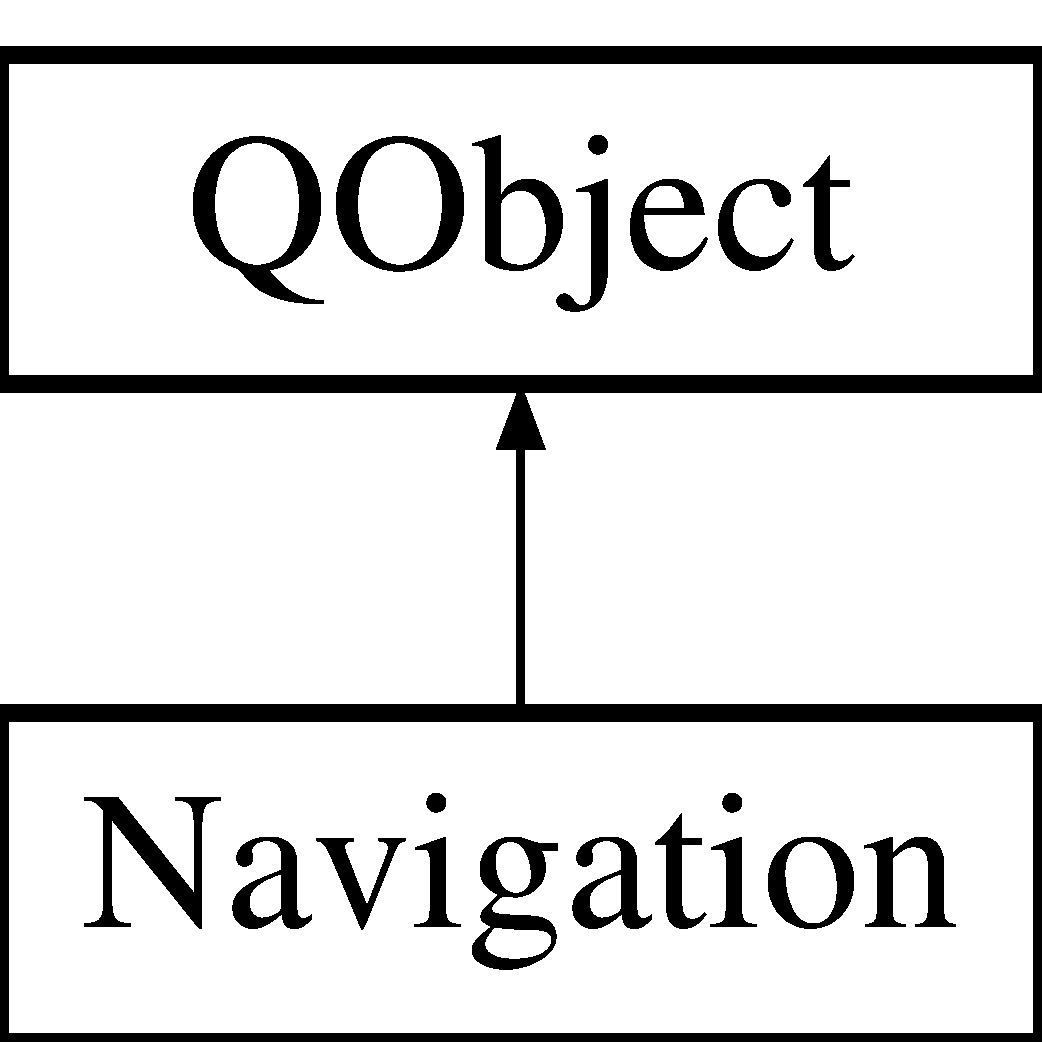
\includegraphics[height=2.000000cm]{class_navigation}
\end{center}
\end{figure}
\subsection*{Signals}
\begin{DoxyCompactItemize}
\item 
void \hyperlink{class_navigation_a46da025077023f9c225d3f5dfe870324}{euler\+Rotation\+Changed} (const Q\+Vector3\+D \&\hyperlink{class_navigation_a264e178e874b62aec38c9986a234d044}{rotation})
\item 
void \hyperlink{class_navigation_ac54fe5d8be2858c2988a9f5158d2d58e}{rotation\+Changed} (const Q\+Quaternion \&\hyperlink{class_navigation_a264e178e874b62aec38c9986a234d044}{rotation})
\item 
void \hyperlink{class_navigation_aa8de8f9227de65da000d1ce730821bab}{world\+Space\+Rotation\+Changed} (const Q\+Quaternion \&\hyperlink{class_navigation_a264e178e874b62aec38c9986a234d044}{rotation})
\end{DoxyCompactItemize}
\subsection*{Public Member Functions}
\begin{DoxyCompactItemize}
\item 
\hyperlink{class_navigation_a9848e09ca6fab3590ffdb0e1c188f31d}{Navigation} (Q\+Object $\ast$parent=0)
\item 
virtual \hyperlink{class_navigation_addd4022d716df48f4e55a1db69361ba7}{$\sim$\+Navigation} ()
\item 
Q\+Quaternion \hyperlink{class_navigation_a264e178e874b62aec38c9986a234d044}{rotation} () const 
\item 
Q\+Quaternion \hyperlink{class_navigation_adedf1fd31c40b2ba7461f67387bbb00c}{world\+Space\+Rotation} () const 
\item 
void \hyperlink{class_navigation_a945e0c9bd30f3c66da040f3242864027}{set\+Camera} (\hyperlink{class_camera}{Camera} $\ast$camera)
\item 
const Q\+Vector3\+D \& \hyperlink{class_navigation_ac756f0b773b771556505a8f20a5f2cf1}{euler\+Rotation} () const 
\item 
void \hyperlink{class_navigation_a4d9b8c12ac091a1db0c3b89f0e36cedd}{set\+Euler\+Rotation} (const Q\+Vector3\+D \&angles)
\end{DoxyCompactItemize}
\subsection*{Protected Member Functions}
\begin{DoxyCompactItemize}
\item 
Q\+Quaternion \hyperlink{class_navigation_a210a31fd6fc626468793b4dbeefcaf2c}{from\+Euler\+Angle\+Quaternions} (const Q\+Quaternion \&x, const Q\+Quaternion \&y, const Q\+Quaternion \&z) const 
\end{DoxyCompactItemize}
\subsection*{Protected Attributes}
\begin{DoxyCompactItemize}
\item 
\hyperlink{class_camera}{Camera} $\ast$ \hyperlink{class_navigation_a76a3e3ea5f8d81a19b22806eb3536302}{m\+\_\+camera}
\item 
Q\+Vector3\+D $\ast$ \hyperlink{class_navigation_a6b056244895c4250c697f6b924874b05}{m\+\_\+euler\+Rotation}
\end{DoxyCompactItemize}


\subsection{Detailed Description}
The \hyperlink{class_navigation}{Navigation} class provides an interface for all navigation techniques.  The navigation takes euler angles in coordinate system based on current view and translate them into quaternions describing the changes in our world. 

\subsection{Constructor \& Destructor Documentation}
\hypertarget{class_navigation_a9848e09ca6fab3590ffdb0e1c188f31d}{\index{Navigation@{Navigation}!Navigation@{Navigation}}
\index{Navigation@{Navigation}!Navigation@{Navigation}}
\subsubsection[{Navigation}]{\setlength{\rightskip}{0pt plus 5cm}Navigation\+::\+Navigation (
\begin{DoxyParamCaption}
\item[{Q\+Object $\ast$}]{parent = {\ttfamily 0}}
\end{DoxyParamCaption}
)\hspace{0.3cm}{\ttfamily [explicit]}}}\label{class_navigation_a9848e09ca6fab3590ffdb0e1c188f31d}
\hypertarget{class_navigation_addd4022d716df48f4e55a1db69361ba7}{\index{Navigation@{Navigation}!````~Navigation@{$\sim$\+Navigation}}
\index{````~Navigation@{$\sim$\+Navigation}!Navigation@{Navigation}}
\subsubsection[{$\sim$\+Navigation}]{\setlength{\rightskip}{0pt plus 5cm}Navigation\+::$\sim$\+Navigation (
\begin{DoxyParamCaption}
{}
\end{DoxyParamCaption}
)\hspace{0.3cm}{\ttfamily [virtual]}}}\label{class_navigation_addd4022d716df48f4e55a1db69361ba7}


\subsection{Member Function Documentation}
\hypertarget{class_navigation_ac756f0b773b771556505a8f20a5f2cf1}{\index{Navigation@{Navigation}!euler\+Rotation@{euler\+Rotation}}
\index{euler\+Rotation@{euler\+Rotation}!Navigation@{Navigation}}
\subsubsection[{euler\+Rotation}]{\setlength{\rightskip}{0pt plus 5cm}const Q\+Vector3\+D\& Navigation\+::euler\+Rotation (
\begin{DoxyParamCaption}
{}
\end{DoxyParamCaption}
) const}}\label{class_navigation_ac756f0b773b771556505a8f20a5f2cf1}
\hypertarget{class_navigation_a46da025077023f9c225d3f5dfe870324}{\index{Navigation@{Navigation}!euler\+Rotation\+Changed@{euler\+Rotation\+Changed}}
\index{euler\+Rotation\+Changed@{euler\+Rotation\+Changed}!Navigation@{Navigation}}
\subsubsection[{euler\+Rotation\+Changed}]{\setlength{\rightskip}{0pt plus 5cm}void Navigation\+::euler\+Rotation\+Changed (
\begin{DoxyParamCaption}
\item[{const Q\+Vector3\+D \&}]{rotation}
\end{DoxyParamCaption}
)\hspace{0.3cm}{\ttfamily [signal]}}}\label{class_navigation_a46da025077023f9c225d3f5dfe870324}
\hypertarget{class_navigation_a210a31fd6fc626468793b4dbeefcaf2c}{\index{Navigation@{Navigation}!from\+Euler\+Angle\+Quaternions@{from\+Euler\+Angle\+Quaternions}}
\index{from\+Euler\+Angle\+Quaternions@{from\+Euler\+Angle\+Quaternions}!Navigation@{Navigation}}
\subsubsection[{from\+Euler\+Angle\+Quaternions}]{\setlength{\rightskip}{0pt plus 5cm}Q\+Quaternion Navigation\+::from\+Euler\+Angle\+Quaternions (
\begin{DoxyParamCaption}
\item[{const Q\+Quaternion \&}]{x, }
\item[{const Q\+Quaternion \&}]{y, }
\item[{const Q\+Quaternion \&}]{z}
\end{DoxyParamCaption}
) const\hspace{0.3cm}{\ttfamily [protected]}}}\label{class_navigation_a210a31fd6fc626468793b4dbeefcaf2c}
\hypertarget{class_navigation_a264e178e874b62aec38c9986a234d044}{\index{Navigation@{Navigation}!rotation@{rotation}}
\index{rotation@{rotation}!Navigation@{Navigation}}
\subsubsection[{rotation}]{\setlength{\rightskip}{0pt plus 5cm}Q\+Quaternion Navigation\+::rotation (
\begin{DoxyParamCaption}
{}
\end{DoxyParamCaption}
) const}}\label{class_navigation_a264e178e874b62aec38c9986a234d044}
\hypertarget{class_navigation_ac54fe5d8be2858c2988a9f5158d2d58e}{\index{Navigation@{Navigation}!rotation\+Changed@{rotation\+Changed}}
\index{rotation\+Changed@{rotation\+Changed}!Navigation@{Navigation}}
\subsubsection[{rotation\+Changed}]{\setlength{\rightskip}{0pt plus 5cm}void Navigation\+::rotation\+Changed (
\begin{DoxyParamCaption}
\item[{const Q\+Quaternion \&}]{rotation}
\end{DoxyParamCaption}
)\hspace{0.3cm}{\ttfamily [signal]}}}\label{class_navigation_ac54fe5d8be2858c2988a9f5158d2d58e}
\hypertarget{class_navigation_a945e0c9bd30f3c66da040f3242864027}{\index{Navigation@{Navigation}!set\+Camera@{set\+Camera}}
\index{set\+Camera@{set\+Camera}!Navigation@{Navigation}}
\subsubsection[{set\+Camera}]{\setlength{\rightskip}{0pt plus 5cm}void Navigation\+::set\+Camera (
\begin{DoxyParamCaption}
\item[{{\bf Camera} $\ast$}]{camera}
\end{DoxyParamCaption}
)}}\label{class_navigation_a945e0c9bd30f3c66da040f3242864027}
\hypertarget{class_navigation_a4d9b8c12ac091a1db0c3b89f0e36cedd}{\index{Navigation@{Navigation}!set\+Euler\+Rotation@{set\+Euler\+Rotation}}
\index{set\+Euler\+Rotation@{set\+Euler\+Rotation}!Navigation@{Navigation}}
\subsubsection[{set\+Euler\+Rotation}]{\setlength{\rightskip}{0pt plus 5cm}void Navigation\+::set\+Euler\+Rotation (
\begin{DoxyParamCaption}
\item[{const Q\+Vector3\+D \&}]{angles}
\end{DoxyParamCaption}
)}}\label{class_navigation_a4d9b8c12ac091a1db0c3b89f0e36cedd}
\hypertarget{class_navigation_adedf1fd31c40b2ba7461f67387bbb00c}{\index{Navigation@{Navigation}!world\+Space\+Rotation@{world\+Space\+Rotation}}
\index{world\+Space\+Rotation@{world\+Space\+Rotation}!Navigation@{Navigation}}
\subsubsection[{world\+Space\+Rotation}]{\setlength{\rightskip}{0pt plus 5cm}Q\+Quaternion Navigation\+::world\+Space\+Rotation (
\begin{DoxyParamCaption}
{}
\end{DoxyParamCaption}
) const}}\label{class_navigation_adedf1fd31c40b2ba7461f67387bbb00c}
\hypertarget{class_navigation_aa8de8f9227de65da000d1ce730821bab}{\index{Navigation@{Navigation}!world\+Space\+Rotation\+Changed@{world\+Space\+Rotation\+Changed}}
\index{world\+Space\+Rotation\+Changed@{world\+Space\+Rotation\+Changed}!Navigation@{Navigation}}
\subsubsection[{world\+Space\+Rotation\+Changed}]{\setlength{\rightskip}{0pt plus 5cm}void Navigation\+::world\+Space\+Rotation\+Changed (
\begin{DoxyParamCaption}
\item[{const Q\+Quaternion \&}]{rotation}
\end{DoxyParamCaption}
)\hspace{0.3cm}{\ttfamily [signal]}}}\label{class_navigation_aa8de8f9227de65da000d1ce730821bab}


\subsection{Member Data Documentation}
\hypertarget{class_navigation_a76a3e3ea5f8d81a19b22806eb3536302}{\index{Navigation@{Navigation}!m\+\_\+camera@{m\+\_\+camera}}
\index{m\+\_\+camera@{m\+\_\+camera}!Navigation@{Navigation}}
\subsubsection[{m\+\_\+camera}]{\setlength{\rightskip}{0pt plus 5cm}{\bf Camera}$\ast$ Navigation\+::m\+\_\+camera\hspace{0.3cm}{\ttfamily [protected]}}}\label{class_navigation_a76a3e3ea5f8d81a19b22806eb3536302}
\hypertarget{class_navigation_a6b056244895c4250c697f6b924874b05}{\index{Navigation@{Navigation}!m\+\_\+euler\+Rotation@{m\+\_\+euler\+Rotation}}
\index{m\+\_\+euler\+Rotation@{m\+\_\+euler\+Rotation}!Navigation@{Navigation}}
\subsubsection[{m\+\_\+euler\+Rotation}]{\setlength{\rightskip}{0pt plus 5cm}Q\+Vector3\+D$\ast$ Navigation\+::m\+\_\+euler\+Rotation\hspace{0.3cm}{\ttfamily [protected]}}}\label{class_navigation_a6b056244895c4250c697f6b924874b05}


The documentation for this class was generated from the following files\+:\begin{DoxyCompactItemize}
\item 
\hyperlink{navigation_8h}{navigation.\+h}\item 
\hyperlink{navigation_8cpp}{navigation.\+cpp}\end{DoxyCompactItemize}

\hypertarget{class_painter}{}\section{Painter Class Reference}
\label{class_painter}\index{Painter@{Painter}}


The \hyperlink{class_painter}{Painter} class  Includes the rendering process, thus creates the whole picture.  




{\ttfamily \#include $<$painter.\+h$>$}

Inheritance diagram for Painter\+:\begin{figure}[H]
\begin{center}
\leavevmode
\includegraphics[height=2.000000cm]{class_painter}
\end{center}
\end{figure}
\subsection*{Public Slots}
\begin{DoxyCompactItemize}
\item 
\hypertarget{class_painter_a5b9b4ed8aebaebeb2f6483e350445fbc}{}void {\bfseries paint} ()\label{class_painter_a5b9b4ed8aebaebeb2f6483e350445fbc}

\end{DoxyCompactItemize}
\subsection*{Public Member Functions}
\begin{DoxyCompactItemize}
\item 
\hypertarget{class_painter_ae9520672fc113fc60cf942ba3d13a46e}{}{\bfseries Painter} (\hyperlink{class_painter_q_m_l}{Painter\+Q\+M\+L} $\ast$painter, Q\+Object $\ast$parent=0)\label{class_painter_ae9520672fc113fc60cf942ba3d13a46e}

\item 
\hypertarget{class_painter_ae2a4d4b93b38b14ca5510b3d66f9752f}{}void {\bfseries initialize\+Envmap} ()\label{class_painter_ae2a4d4b93b38b14ca5510b3d66f9752f}

\item 
\hypertarget{class_painter_addfa0fd4dd943d27c67b62dfc9ab3a0b}{}bool {\bfseries is\+Active} () const \label{class_painter_addfa0fd4dd943d27c67b62dfc9ab3a0b}

\item 
\hypertarget{class_painter_a7dd43be8d3e1eab98035fcc23316bd1a}{}void {\bfseries set\+Active} (bool active)\label{class_painter_a7dd43be8d3e1eab98035fcc23316bd1a}

\item 
\hypertarget{class_painter_ae666ca89f52438dd898054a38cb7678c}{}void {\bfseries set\+Camera} (const \hyperlink{class_camera}{Camera} \&camera)\label{class_painter_ae666ca89f52438dd898054a38cb7678c}

\item 
\hypertarget{class_painter_a9a306e3a17dcd709a1e23faf8b28cab3}{}\hyperlink{class_scene}{Scene} $\ast$ {\bfseries scene} () const \label{class_painter_a9a306e3a17dcd709a1e23faf8b28cab3}

\item 
\hypertarget{class_painter_ad0c60a921518aac36ecbbf9c050bb779}{}void {\bfseries set\+Scene} (\hyperlink{class_scene}{Scene} $\ast$scene)\label{class_painter_ad0c60a921518aac36ecbbf9c050bb779}

\item 
void \hyperlink{class_painter_a6cbe31709ecd794c00d4c524c8468b14}{set\+Viewport} (const Q\+Size \&viewport)
\begin{DoxyCompactList}\small\item\em Scene\+Renderer\+::set\+Viewport Only set within sync() \end{DoxyCompactList}\item 
\hypertarget{class_painter_a3a8ffdc1e2408e267717ed3816e93e19}{}Q\+String {\bfseries env\+Map\+Prefix} () const \label{class_painter_a3a8ffdc1e2408e267717ed3816e93e19}

\item 
\hypertarget{class_painter_afb568401ef2792e27e4f565bf35cb6bb}{}void {\bfseries set\+Env\+Map\+Prefix} (const Q\+String \&env\+Map\+Prefix)\label{class_painter_afb568401ef2792e27e4f565bf35cb6bb}

\item 
\hypertarget{class_painter_a0c2b82efd3882c162d9807282aab189f}{}Q\+Open\+G\+L\+Functions \& {\bfseries gl} () const \label{class_painter_a0c2b82efd3882c162d9807282aab189f}

\end{DoxyCompactItemize}
\subsection*{Protected Member Functions}
\begin{DoxyCompactItemize}
\item 
\hypertarget{class_painter_a12f9623c2acf87eced6e141e7638804e}{}void {\bfseries initialize} ()\label{class_painter_a12f9623c2acf87eced6e141e7638804e}

\item 
\hypertarget{class_painter_a3deca470f67f8e9fafc0cc901c689c02}{}void {\bfseries paint\+Envmap} ()\label{class_painter_a3deca470f67f8e9fafc0cc901c689c02}

\end{DoxyCompactItemize}
\subsection*{Protected Attributes}
\begin{DoxyCompactItemize}
\item 
\hypertarget{class_painter_a9b476c949ca4b2af7b1653c7106b659b}{}bool {\bfseries m\+\_\+active}\label{class_painter_a9b476c949ca4b2af7b1653c7106b659b}

\item 
\hypertarget{class_painter_a05558ea7a2f818641e0506d01d518010}{}\hyperlink{class_camera}{Camera} $\ast$ {\bfseries m\+\_\+camera}\label{class_painter_a05558ea7a2f818641e0506d01d518010}

\item 
\hypertarget{class_painter_a141349e5459cd3ce52bb12b85579f752}{}uint {\bfseries m\+\_\+envmap}\label{class_painter_a141349e5459cd3ce52bb12b85579f752}

\item 
\hypertarget{class_painter_a983045c9611224d2576cf1d20fb87770}{}Q\+String {\bfseries m\+\_\+env\+Map\+Prefix}\label{class_painter_a983045c9611224d2576cf1d20fb87770}

\item 
\hypertarget{class_painter_a8aa44a5f1477d570ee10d3dacae09f08}{}Q\+Open\+G\+L\+Functions $\ast$ {\bfseries m\+\_\+gl}\label{class_painter_a8aa44a5f1477d570ee10d3dacae09f08}

\item 
\hypertarget{class_painter_a0adcfafb8172b4f76561e2c951b1090b}{}bool {\bfseries m\+\_\+initialized}\label{class_painter_a0adcfafb8172b4f76561e2c951b1090b}

\item 
\hypertarget{class_painter_af2774293bfaf6f654cb01e504937abb8}{}\hyperlink{class_painter_q_m_l}{Painter\+Q\+M\+L} $\ast$ {\bfseries m\+\_\+painter\+Q\+M\+L}\label{class_painter_af2774293bfaf6f654cb01e504937abb8}

\item 
\hypertarget{class_painter_a50f7fad2d44554f0be878a96afacfa44}{}\hyperlink{class_screen_aligned_quad}{Screen\+Aligned\+Quad} $\ast$ {\bfseries m\+\_\+quad}\label{class_painter_a50f7fad2d44554f0be878a96afacfa44}

\item 
\hypertarget{class_painter_a9aa927a8a72482a508d5abd8e4f7d590}{}\hyperlink{class_scene}{Scene} $\ast$ {\bfseries m\+\_\+scene}\label{class_painter_a9aa927a8a72482a508d5abd8e4f7d590}

\item 
\hypertarget{class_painter_ac1208fd08f67613750efb7adbb718cea}{}Q\+Map$<$ Shader\+Programs, Q\+Open\+G\+L\+Shader\+Program $\ast$ $>$ $\ast$ {\bfseries m\+\_\+shader\+Programs}\label{class_painter_ac1208fd08f67613750efb7adbb718cea}

\item 
\hypertarget{class_painter_a9369e3a89f7074d7fae461acb18adf45}{}Q\+Size $\ast$ {\bfseries m\+\_\+viewport}\label{class_painter_a9369e3a89f7074d7fae461acb18adf45}

\end{DoxyCompactItemize}


\subsection{Detailed Description}
The \hyperlink{class_painter}{Painter} class  Includes the rendering process, thus creates the whole picture. 

\subsection{Member Function Documentation}
\hypertarget{class_painter_a6cbe31709ecd794c00d4c524c8468b14}{}\index{Painter@{Painter}!set\+Viewport@{set\+Viewport}}
\index{set\+Viewport@{set\+Viewport}!Painter@{Painter}}
\subsubsection[{set\+Viewport}]{\setlength{\rightskip}{0pt plus 5cm}void Painter\+::set\+Viewport (
\begin{DoxyParamCaption}
\item[{const Q\+Size \&}]{viewport}
\end{DoxyParamCaption}
)}\label{class_painter_a6cbe31709ecd794c00d4c524c8468b14}


Scene\+Renderer\+::set\+Viewport Only set within sync() 


\begin{DoxyParams}{Parameters}
{\em viewport} & \\
\hline
\end{DoxyParams}


The documentation for this class was generated from the following files\+:\begin{DoxyCompactItemize}
\item 
gem\+Illuminator/painter.\+h\item 
gem\+Illuminator/painter.\+cpp\end{DoxyCompactItemize}

\hypertarget{class_painter_q_m_l}{}\section{Painter\+Q\+M\+L Class Reference}
\label{class_painter_q_m_l}\index{Painter\+Q\+M\+L@{Painter\+Q\+M\+L}}
Inheritance diagram for Painter\+Q\+M\+L\+:\begin{figure}[H]
\begin{center}
\leavevmode
\includegraphics[height=2.000000cm]{class_painter_q_m_l}
\end{center}
\end{figure}
\subsection*{Public Slots}
\begin{DoxyCompactItemize}
\item 
\hypertarget{class_painter_q_m_l_a4cfd22a52fc9e29d304c0ff7cea86744}{}void {\bfseries synchronize} ()\label{class_painter_q_m_l_a4cfd22a52fc9e29d304c0ff7cea86744}

\item 
\hypertarget{class_painter_q_m_l_ab07e4719d2b05bbbfa48980b4854d190}{}void {\bfseries cleanup} ()\label{class_painter_q_m_l_ab07e4719d2b05bbbfa48980b4854d190}

\end{DoxyCompactItemize}
\subsection*{Signals}
\begin{DoxyCompactItemize}
\item 
\hypertarget{class_painter_q_m_l_a90dae96b602fc324b707ffd56d2bb3d8}{}void {\bfseries active\+Changed} ()\label{class_painter_q_m_l_a90dae96b602fc324b707ffd56d2bb3d8}

\item 
\hypertarget{class_painter_q_m_l_a5fce3441beea885f9ba2a70b2f21f0ae}{}void {\bfseries scene\+Changed} ()\label{class_painter_q_m_l_a5fce3441beea885f9ba2a70b2f21f0ae}

\item 
\hypertarget{class_painter_q_m_l_ab7b3f62ef3f2bcbea8b215d4cfb859cd}{}void {\bfseries env\+Map\+Prefix\+Changed} ()\label{class_painter_q_m_l_ab7b3f62ef3f2bcbea8b215d4cfb859cd}

\end{DoxyCompactItemize}
\subsection*{Public Member Functions}
\begin{DoxyCompactItemize}
\item 
\hypertarget{class_painter_q_m_l_a6ce68afc41c75b1fc74da16890d9f797}{}{\bfseries Painter\+Q\+M\+L} (Q\+Quick\+Item $\ast$parent=0)\label{class_painter_q_m_l_a6ce68afc41c75b1fc74da16890d9f797}

\item 
\hypertarget{class_painter_q_m_l_af5c04e89584445a002e7a86d6ab071c3}{}Q\+String {\bfseries env\+Map\+Prefix} () const \label{class_painter_q_m_l_af5c04e89584445a002e7a86d6ab071c3}

\item 
\hypertarget{class_painter_q_m_l_a65bd9e19f9b6b1bd197c34d3a9174f04}{}void {\bfseries set\+Env\+Map\+Prefix} (const Q\+String \&env\+Map\+Prefix)\label{class_painter_q_m_l_a65bd9e19f9b6b1bd197c34d3a9174f04}

\item 
\hypertarget{class_painter_q_m_l_a69fecccc6056c3ee957219ffd63c193c}{}bool {\bfseries event} (Q\+Event $\ast$ev) override\label{class_painter_q_m_l_a69fecccc6056c3ee957219ffd63c193c}

\item 
\hypertarget{class_painter_q_m_l_a391bd3c26f57dfcb3177318595c89353}{}bool {\bfseries is\+Active} () const \label{class_painter_q_m_l_a391bd3c26f57dfcb3177318595c89353}

\item 
\hypertarget{class_painter_q_m_l_a242301828022a572c1f1b72eb3ecd9e5}{}void {\bfseries set\+Active} (bool active)\label{class_painter_q_m_l_a242301828022a572c1f1b72eb3ecd9e5}

\item 
\hypertarget{class_painter_q_m_l_a7715bb2f3d638ff3d5e6e602a427b413}{}Q\+Event\+::\+Type {\bfseries painting\+Done\+Event\+Type} ()\label{class_painter_q_m_l_a7715bb2f3d638ff3d5e6e602a427b413}

\item 
\hypertarget{class_painter_q_m_l_a6694ad2cfda4aefaffc0a3151a2b09dd}{}\hyperlink{class_scene}{Scene} $\ast$ {\bfseries scene} () const \label{class_painter_q_m_l_a6694ad2cfda4aefaffc0a3151a2b09dd}

\item 
\hypertarget{class_painter_q_m_l_a81288bcb25e5b985eea33b26ede7931a}{}void {\bfseries set\+Scene} (\hyperlink{class_scene}{Scene} $\ast$scene)\label{class_painter_q_m_l_a81288bcb25e5b985eea33b26ede7931a}

\end{DoxyCompactItemize}
\subsection*{Protected Attributes}
\begin{DoxyCompactItemize}
\item 
\hypertarget{class_painter_q_m_l_af2f0bd70fd315e03ea7b8e9275bf0012}{}bool {\bfseries m\+\_\+active}\label{class_painter_q_m_l_af2f0bd70fd315e03ea7b8e9275bf0012}

\item 
\hypertarget{class_painter_q_m_l_a3b291f7043ad8437baadf6d7be1c174d}{}bool {\bfseries m\+\_\+is\+Update\+Pending}\label{class_painter_q_m_l_a3b291f7043ad8437baadf6d7be1c174d}

\item 
\hypertarget{class_painter_q_m_l_a60f7fcbca84633e58f2facb4b805c494}{}Q\+String {\bfseries m\+\_\+env\+Map\+Prefix}\label{class_painter_q_m_l_a60f7fcbca84633e58f2facb4b805c494}

\item 
\hypertarget{class_painter_q_m_l_ac4cdaa622f2b608a364051f06d3f9d18}{}bool {\bfseries m\+\_\+is\+Env\+Map\+Invalidated}\label{class_painter_q_m_l_ac4cdaa622f2b608a364051f06d3f9d18}

\item 
\hypertarget{class_painter_q_m_l_a6b21bae1a75260e121bc56cda38729c8}{}\hyperlink{class_painter}{Painter} $\ast$ {\bfseries m\+\_\+painter}\label{class_painter_q_m_l_a6b21bae1a75260e121bc56cda38729c8}

\item 
\hypertarget{class_painter_q_m_l_a7a6641710573e4fa47dfdae13e87d58e}{}int {\bfseries m\+\_\+painting\+Done\+Event\+Type}\label{class_painter_q_m_l_a7a6641710573e4fa47dfdae13e87d58e}

\item 
\hypertarget{class_painter_q_m_l_a5eccac2ab6d9974a9ae94573ac7b19d6}{}\hyperlink{class_scene}{Scene} $\ast$ {\bfseries m\+\_\+scene}\label{class_painter_q_m_l_a5eccac2ab6d9974a9ae94573ac7b19d6}

\item 
\hypertarget{class_painter_q_m_l_ad4ced718f47b69f2344a5311ec87a156}{}Q\+Time $\ast$ {\bfseries m\+\_\+time}\label{class_painter_q_m_l_ad4ced718f47b69f2344a5311ec87a156}

\end{DoxyCompactItemize}
\subsection*{Properties}
\begin{DoxyCompactItemize}
\item 
\hypertarget{class_painter_q_m_l_ae3e2f50a3b7fc1d136f408a2b6745e73}{}bool {\bfseries active}\label{class_painter_q_m_l_ae3e2f50a3b7fc1d136f408a2b6745e73}

\item 
\hypertarget{class_painter_q_m_l_ab9c17177ba01d52fcc85606cd18cc3fe}{}Q\+String {\bfseries env\+Map\+Prefix}\label{class_painter_q_m_l_ab9c17177ba01d52fcc85606cd18cc3fe}

\item 
\hypertarget{class_painter_q_m_l_a59b4d398bc7880e59bc8296c2669aaab}{}\hyperlink{class_scene}{Scene} {\bfseries scene}\label{class_painter_q_m_l_a59b4d398bc7880e59bc8296c2669aaab}

\end{DoxyCompactItemize}


The documentation for this class was generated from the following files\+:\begin{DoxyCompactItemize}
\item 
gem\+Illuminator/painterqml.\+h\item 
gem\+Illuminator/painterqml.\+cpp\end{DoxyCompactItemize}

\hypertarget{class_player}{}\section{Player Class Reference}
\label{class_player}\index{Player@{Player}}


Our \hyperlink{class_player}{Player} class is pretty stupid, because our player only ride on lightrays. The only responsiblity is to move on rays and update the camera.  




{\ttfamily \#include $<$player.\+h$>$}

Inheritance diagram for Player\+:\begin{figure}[H]
\begin{center}
\leavevmode
\includegraphics[height=2.000000cm]{class_player}
\end{center}
\end{figure}
\subsection*{Public Slots}
\begin{DoxyCompactItemize}
\item 
\hyperlink{class_camera}{Camera} $\ast$ \hyperlink{class_player_a10605ebcab0fac1b542d1bd8f3d23acd}{camera} () const 
\begin{DoxyCompactList}\small\item\em The camera which is updated by player. \end{DoxyCompactList}\item 
void \hyperlink{class_player_af5e57b3a9719cd999aff21d59355be52}{set\+Camera} (\hyperlink{class_camera}{Camera} $\ast$\hyperlink{class_player_a4e1ae30bdaec837b94451416a523d5cb}{camera})
\begin{DoxyCompactList}\small\item\em Sets the camera, that should be updated by player. The player does not take ownership of camera. \end{DoxyCompactList}\item 
qreal \hyperlink{class_player_a836e1afdde2c379b964bcf5d3811f0da}{velocity} () const 
\begin{DoxyCompactList}\small\item\em The velocity of player. \end{DoxyCompactList}\item 
void \hyperlink{class_player_ae2d5423c7bf6c6c924a451dc1cdab6aa}{set\+Velocity} (qreal \hyperlink{class_player_a53141a3791c456938945973cc78a2ea7}{velocity})
\begin{DoxyCompactList}\small\item\em Set velocity of player. \end{DoxyCompactList}\end{DoxyCompactItemize}
\subsection*{Signals}
\begin{DoxyCompactItemize}
\item 
void \hyperlink{class_player_aef620bc75871b32311560a7b2a31c144}{camera\+Changed} ()
\item 
void \hyperlink{class_player_a22ae3d9604e92fa12cfad39fe40e8651}{velocity\+Changed} ()
\end{DoxyCompactItemize}
\subsection*{Public Member Functions}
\begin{DoxyCompactItemize}
\item 
\hyperlink{class_player_a5c2a46dbacbc28b7cfbe352b6c0db644}{Player} (Q\+Object $\ast$parent=0)
\item 
virtual \hyperlink{class_player_a749d2c00e1fe0f5c2746f7505a58c062}{$\sim$\+Player} ()
\item 
void \hyperlink{class_player_a6dcd0b9f4d678260314878ab20ce6e09}{move\+On\+Ray} (const \hyperlink{class_light_ray}{Light\+Ray} \&ray, int time\+Difference\+In\+Milliseconds)
\begin{DoxyCompactList}\small\item\em Move the player along a ray. \end{DoxyCompactList}\item 
void \hyperlink{class_player_a38269e0706f91b71c6e8f8373c397969}{move\+To\+Start\+Point\+On\+Ray} (const \hyperlink{class_light_ray}{Light\+Ray} \&ray)
\begin{DoxyCompactList}\small\item\em Set the player to ray.\+start\+Position() and updates the camera accordingly. \end{DoxyCompactList}\item 
void \hyperlink{class_player_a0a4ebefb0f7593d79573ddcfe68e8e2f}{move\+To\+End\+Point\+On\+Ray} (const \hyperlink{class_light_ray}{Light\+Ray} \&ray)
\begin{DoxyCompactList}\small\item\em Set the player to ray.\+end\+Position() and updates the camera accordingly. \end{DoxyCompactList}\item 
const Q\+Vector3\+D \& \hyperlink{class_player_a0c307c67d3c6d64ee9c5b724c1e2b095}{position} () const 
\begin{DoxyCompactList}\small\item\em The position of player in world coordinates. \end{DoxyCompactList}\item 
void \hyperlink{class_player_a0cb33ddb87038b4e2af648e1b884d79f}{set\+Position} (const Q\+Vector3\+D \&\hyperlink{class_player_a0c307c67d3c6d64ee9c5b724c1e2b095}{position})
\item 
void \hyperlink{class_player_ae51ad40372e26d33351c02d77a1aba63}{set\+View\+Direction} (const Q\+Vector3\+D \&view\+Direction)
\begin{DoxyCompactList}\small\item\em Set view direction to provided value. For now this value should be the same like the direction of followed lightray. \end{DoxyCompactList}\end{DoxyCompactItemize}
\subsection*{Protected Member Functions}
\begin{DoxyCompactItemize}
\item 
void \hyperlink{class_player_a557b70acbd3cb1f71218390f7e90105c}{update\+Camera\+For\+Point\+On\+Ray} (const Q\+Vector3\+D \&point, const \hyperlink{class_light_ray}{Light\+Ray} \&ray)
\begin{DoxyCompactList}\small\item\em Updates the camera position for given point on ray. \end{DoxyCompactList}\end{DoxyCompactItemize}
\subsection*{Protected Attributes}
\begin{DoxyCompactItemize}
\item 
qreal \hyperlink{class_player_a962e97e5fd3fe1c2db4e7e2066dbe61c}{m\+\_\+velocity}
\item 
Q\+Vector3\+D $\ast$ \hyperlink{class_player_a9dc251e6a6d9a7f49c3f2ad5b64a7780}{m\+\_\+position}
\item 
\hyperlink{class_camera}{Camera} $\ast$ \hyperlink{class_player_a7721626a1c43592bfcb0c81a836f7aad}{m\+\_\+camera}
\end{DoxyCompactItemize}
\subsection*{Properties}
\begin{DoxyCompactItemize}
\item 
\hyperlink{class_camera}{Camera} \hyperlink{class_player_a4e1ae30bdaec837b94451416a523d5cb}{camera}
\item 
qreal \hyperlink{class_player_a53141a3791c456938945973cc78a2ea7}{velocity}
\end{DoxyCompactItemize}


\subsection{Detailed Description}
Our \hyperlink{class_player}{Player} class is pretty stupid, because our player only ride on lightrays. The only responsiblity is to move on rays and update the camera. 

\subsection{Constructor \& Destructor Documentation}
\hypertarget{class_player_a5c2a46dbacbc28b7cfbe352b6c0db644}{}\index{Player@{Player}!Player@{Player}}
\index{Player@{Player}!Player@{Player}}
\subsubsection[{Player}]{\setlength{\rightskip}{0pt plus 5cm}Player\+::\+Player (
\begin{DoxyParamCaption}
\item[{Q\+Object $\ast$}]{parent = {\ttfamily 0}}
\end{DoxyParamCaption}
)\hspace{0.3cm}{\ttfamily [explicit]}}\label{class_player_a5c2a46dbacbc28b7cfbe352b6c0db644}
\hypertarget{class_player_a749d2c00e1fe0f5c2746f7505a58c062}{}\index{Player@{Player}!````~Player@{$\sim$\+Player}}
\index{````~Player@{$\sim$\+Player}!Player@{Player}}
\subsubsection[{$\sim$\+Player}]{\setlength{\rightskip}{0pt plus 5cm}Player\+::$\sim$\+Player (
\begin{DoxyParamCaption}
{}
\end{DoxyParamCaption}
)\hspace{0.3cm}{\ttfamily [virtual]}}\label{class_player_a749d2c00e1fe0f5c2746f7505a58c062}


\subsection{Member Function Documentation}
\hypertarget{class_player_a10605ebcab0fac1b542d1bd8f3d23acd}{}\index{Player@{Player}!camera@{camera}}
\index{camera@{camera}!Player@{Player}}
\subsubsection[{camera}]{\setlength{\rightskip}{0pt plus 5cm}{\bf Camera}$\ast$ Player\+::camera (
\begin{DoxyParamCaption}
{}
\end{DoxyParamCaption}
) const\hspace{0.3cm}{\ttfamily [slot]}}\label{class_player_a10605ebcab0fac1b542d1bd8f3d23acd}


The camera which is updated by player. 

\begin{DoxyReturn}{Returns}

\end{DoxyReturn}
\hypertarget{class_player_aef620bc75871b32311560a7b2a31c144}{}\index{Player@{Player}!camera\+Changed@{camera\+Changed}}
\index{camera\+Changed@{camera\+Changed}!Player@{Player}}
\subsubsection[{camera\+Changed}]{\setlength{\rightskip}{0pt plus 5cm}void Player\+::camera\+Changed (
\begin{DoxyParamCaption}
{}
\end{DoxyParamCaption}
)\hspace{0.3cm}{\ttfamily [signal]}}\label{class_player_aef620bc75871b32311560a7b2a31c144}
\hypertarget{class_player_a6dcd0b9f4d678260314878ab20ce6e09}{}\index{Player@{Player}!move\+On\+Ray@{move\+On\+Ray}}
\index{move\+On\+Ray@{move\+On\+Ray}!Player@{Player}}
\subsubsection[{move\+On\+Ray}]{\setlength{\rightskip}{0pt plus 5cm}void Player\+::move\+On\+Ray (
\begin{DoxyParamCaption}
\item[{const {\bf Light\+Ray} \&}]{ray, }
\item[{int}]{time\+Difference\+In\+Milliseconds}
\end{DoxyParamCaption}
)}\label{class_player_a6dcd0b9f4d678260314878ab20ce6e09}


Move the player along a ray. 


\begin{DoxyParams}{Parameters}
{\em ray} & The ray that is followed by ray. \\
\hline
{\em time\+Difference\+In\+Milliseconds} & The time left since last update in order to calculate how far the player should move. \\
\hline
\end{DoxyParams}
\hypertarget{class_player_a0a4ebefb0f7593d79573ddcfe68e8e2f}{}\index{Player@{Player}!move\+To\+End\+Point\+On\+Ray@{move\+To\+End\+Point\+On\+Ray}}
\index{move\+To\+End\+Point\+On\+Ray@{move\+To\+End\+Point\+On\+Ray}!Player@{Player}}
\subsubsection[{move\+To\+End\+Point\+On\+Ray}]{\setlength{\rightskip}{0pt plus 5cm}void Player\+::move\+To\+End\+Point\+On\+Ray (
\begin{DoxyParamCaption}
\item[{const {\bf Light\+Ray} \&}]{ray}
\end{DoxyParamCaption}
)}\label{class_player_a0a4ebefb0f7593d79573ddcfe68e8e2f}


Set the player to ray.\+end\+Position() and updates the camera accordingly. 


\begin{DoxyParams}{Parameters}
{\em ray} & \hyperlink{class_player_a0a4ebefb0f7593d79573ddcfe68e8e2f}{move\+To\+End\+Point\+On\+Ray()}; \\
\hline
\end{DoxyParams}
\hypertarget{class_player_a38269e0706f91b71c6e8f8373c397969}{}\index{Player@{Player}!move\+To\+Start\+Point\+On\+Ray@{move\+To\+Start\+Point\+On\+Ray}}
\index{move\+To\+Start\+Point\+On\+Ray@{move\+To\+Start\+Point\+On\+Ray}!Player@{Player}}
\subsubsection[{move\+To\+Start\+Point\+On\+Ray}]{\setlength{\rightskip}{0pt plus 5cm}void Player\+::move\+To\+Start\+Point\+On\+Ray (
\begin{DoxyParamCaption}
\item[{const {\bf Light\+Ray} \&}]{ray}
\end{DoxyParamCaption}
)}\label{class_player_a38269e0706f91b71c6e8f8373c397969}


Set the player to ray.\+start\+Position() and updates the camera accordingly. 


\begin{DoxyParams}{Parameters}
{\em ray} & \hyperlink{class_player_a0a4ebefb0f7593d79573ddcfe68e8e2f}{move\+To\+End\+Point\+On\+Ray()}; \\
\hline
\end{DoxyParams}
\hypertarget{class_player_a0c307c67d3c6d64ee9c5b724c1e2b095}{}\index{Player@{Player}!position@{position}}
\index{position@{position}!Player@{Player}}
\subsubsection[{position}]{\setlength{\rightskip}{0pt plus 5cm}const Q\+Vector3\+D \& Player\+::position (
\begin{DoxyParamCaption}
{}
\end{DoxyParamCaption}
) const}\label{class_player_a0c307c67d3c6d64ee9c5b724c1e2b095}


The position of player in world coordinates. 

\begin{DoxyReturn}{Returns}

\end{DoxyReturn}
\hypertarget{class_player_af5e57b3a9719cd999aff21d59355be52}{}\index{Player@{Player}!set\+Camera@{set\+Camera}}
\index{set\+Camera@{set\+Camera}!Player@{Player}}
\subsubsection[{set\+Camera}]{\setlength{\rightskip}{0pt plus 5cm}void Player\+::set\+Camera (
\begin{DoxyParamCaption}
\item[{{\bf Camera} $\ast$}]{camera}
\end{DoxyParamCaption}
)\hspace{0.3cm}{\ttfamily [slot]}}\label{class_player_af5e57b3a9719cd999aff21d59355be52}


Sets the camera, that should be updated by player. The player does not take ownership of camera. 


\begin{DoxyParams}{Parameters}
{\em camera} & \\
\hline
\end{DoxyParams}
\hypertarget{class_player_a0cb33ddb87038b4e2af648e1b884d79f}{}\index{Player@{Player}!set\+Position@{set\+Position}}
\index{set\+Position@{set\+Position}!Player@{Player}}
\subsubsection[{set\+Position}]{\setlength{\rightskip}{0pt plus 5cm}void Player\+::set\+Position (
\begin{DoxyParamCaption}
\item[{const Q\+Vector3\+D \&}]{position}
\end{DoxyParamCaption}
)}\label{class_player_a0cb33ddb87038b4e2af648e1b884d79f}
\hypertarget{class_player_ae2d5423c7bf6c6c924a451dc1cdab6aa}{}\index{Player@{Player}!set\+Velocity@{set\+Velocity}}
\index{set\+Velocity@{set\+Velocity}!Player@{Player}}
\subsubsection[{set\+Velocity}]{\setlength{\rightskip}{0pt plus 5cm}void Player\+::set\+Velocity (
\begin{DoxyParamCaption}
\item[{qreal}]{velocity}
\end{DoxyParamCaption}
)\hspace{0.3cm}{\ttfamily [slot]}}\label{class_player_ae2d5423c7bf6c6c924a451dc1cdab6aa}


Set velocity of player. 


\begin{DoxyParams}{Parameters}
{\em velocity} & \\
\hline
\end{DoxyParams}
\hypertarget{class_player_ae51ad40372e26d33351c02d77a1aba63}{}\index{Player@{Player}!set\+View\+Direction@{set\+View\+Direction}}
\index{set\+View\+Direction@{set\+View\+Direction}!Player@{Player}}
\subsubsection[{set\+View\+Direction}]{\setlength{\rightskip}{0pt plus 5cm}void Player\+::set\+View\+Direction (
\begin{DoxyParamCaption}
\item[{const Q\+Vector3\+D \&}]{view\+Direction}
\end{DoxyParamCaption}
)}\label{class_player_ae51ad40372e26d33351c02d77a1aba63}


Set view direction to provided value. For now this value should be the same like the direction of followed lightray. 


\begin{DoxyParams}{Parameters}
{\em view\+Direction} & \\
\hline
\end{DoxyParams}
\hypertarget{class_player_a557b70acbd3cb1f71218390f7e90105c}{}\index{Player@{Player}!update\+Camera\+For\+Point\+On\+Ray@{update\+Camera\+For\+Point\+On\+Ray}}
\index{update\+Camera\+For\+Point\+On\+Ray@{update\+Camera\+For\+Point\+On\+Ray}!Player@{Player}}
\subsubsection[{update\+Camera\+For\+Point\+On\+Ray}]{\setlength{\rightskip}{0pt plus 5cm}void Player\+::update\+Camera\+For\+Point\+On\+Ray (
\begin{DoxyParamCaption}
\item[{const Q\+Vector3\+D \&}]{point, }
\item[{const {\bf Light\+Ray} \&}]{ray}
\end{DoxyParamCaption}
)\hspace{0.3cm}{\ttfamily [protected]}}\label{class_player_a557b70acbd3cb1f71218390f7e90105c}


Updates the camera position for given point on ray. 


\begin{DoxyParams}{Parameters}
{\em point} & The new \hyperlink{class_player_a0c307c67d3c6d64ee9c5b724c1e2b095}{position()} of player on ray. This point has to lie on ray or it will lead to unexpected behaviour \\
\hline
{\em ray} & The lightray the player is following. \\
\hline
\end{DoxyParams}
\hypertarget{class_player_a836e1afdde2c379b964bcf5d3811f0da}{}\index{Player@{Player}!velocity@{velocity}}
\index{velocity@{velocity}!Player@{Player}}
\subsubsection[{velocity}]{\setlength{\rightskip}{0pt plus 5cm}qreal Player\+::velocity (
\begin{DoxyParamCaption}
{}
\end{DoxyParamCaption}
) const\hspace{0.3cm}{\ttfamily [slot]}}\label{class_player_a836e1afdde2c379b964bcf5d3811f0da}


The velocity of player. 

\begin{DoxyReturn}{Returns}
Returns the distance, that is passed in one second. 
\end{DoxyReturn}
\hypertarget{class_player_a22ae3d9604e92fa12cfad39fe40e8651}{}\index{Player@{Player}!velocity\+Changed@{velocity\+Changed}}
\index{velocity\+Changed@{velocity\+Changed}!Player@{Player}}
\subsubsection[{velocity\+Changed}]{\setlength{\rightskip}{0pt plus 5cm}void Player\+::velocity\+Changed (
\begin{DoxyParamCaption}
{}
\end{DoxyParamCaption}
)\hspace{0.3cm}{\ttfamily [signal]}}\label{class_player_a22ae3d9604e92fa12cfad39fe40e8651}


\subsection{Member Data Documentation}
\hypertarget{class_player_a7721626a1c43592bfcb0c81a836f7aad}{}\index{Player@{Player}!m\+\_\+camera@{m\+\_\+camera}}
\index{m\+\_\+camera@{m\+\_\+camera}!Player@{Player}}
\subsubsection[{m\+\_\+camera}]{\setlength{\rightskip}{0pt plus 5cm}{\bf Camera}$\ast$ Player\+::m\+\_\+camera\hspace{0.3cm}{\ttfamily [protected]}}\label{class_player_a7721626a1c43592bfcb0c81a836f7aad}
\hypertarget{class_player_a9dc251e6a6d9a7f49c3f2ad5b64a7780}{}\index{Player@{Player}!m\+\_\+position@{m\+\_\+position}}
\index{m\+\_\+position@{m\+\_\+position}!Player@{Player}}
\subsubsection[{m\+\_\+position}]{\setlength{\rightskip}{0pt plus 5cm}Q\+Vector3\+D$\ast$ Player\+::m\+\_\+position\hspace{0.3cm}{\ttfamily [protected]}}\label{class_player_a9dc251e6a6d9a7f49c3f2ad5b64a7780}
\hypertarget{class_player_a962e97e5fd3fe1c2db4e7e2066dbe61c}{}\index{Player@{Player}!m\+\_\+velocity@{m\+\_\+velocity}}
\index{m\+\_\+velocity@{m\+\_\+velocity}!Player@{Player}}
\subsubsection[{m\+\_\+velocity}]{\setlength{\rightskip}{0pt plus 5cm}qreal Player\+::m\+\_\+velocity\hspace{0.3cm}{\ttfamily [protected]}}\label{class_player_a962e97e5fd3fe1c2db4e7e2066dbe61c}


\subsection{Property Documentation}
\hypertarget{class_player_a4e1ae30bdaec837b94451416a523d5cb}{}\index{Player@{Player}!camera@{camera}}
\index{camera@{camera}!Player@{Player}}
\subsubsection[{camera}]{\setlength{\rightskip}{0pt plus 5cm}{\bf Camera} $\ast$ Player\+::camera\hspace{0.3cm}{\ttfamily [read]}, {\ttfamily [write]}}\label{class_player_a4e1ae30bdaec837b94451416a523d5cb}
\hypertarget{class_player_a53141a3791c456938945973cc78a2ea7}{}\index{Player@{Player}!velocity@{velocity}}
\index{velocity@{velocity}!Player@{Player}}
\subsubsection[{velocity}]{\setlength{\rightskip}{0pt plus 5cm}qreal Player\+::velocity\hspace{0.3cm}{\ttfamily [read]}, {\ttfamily [write]}}\label{class_player_a53141a3791c456938945973cc78a2ea7}


The documentation for this class was generated from the following files\+:\begin{DoxyCompactItemize}
\item 
Game-\/\+Programming-\/\+W\+S2014/gem\+Illuminator/\hyperlink{player_8h}{player.\+h}\item 
Game-\/\+Programming-\/\+W\+S2014/gem\+Illuminator/\hyperlink{player_8cpp}{player.\+cpp}\end{DoxyCompactItemize}

\hypertarget{singleton_q_hash}{\section{Q\+Hash$<$ Key, T $>$ Singleton Reference}
\label{singleton_q_hash}\index{Q\+Hash$<$ Key, T $>$@{Q\+Hash$<$ Key, T $>$}}
}


{\ttfamily \#include $<$gemrenderer.\+h$>$}



The documentation for this singleton was generated from the following file\+:\begin{DoxyCompactItemize}
\item 
\hyperlink{gemrenderer_8h}{gemrenderer.\+h}\end{DoxyCompactItemize}

\hypertarget{singleton_q_list}{\section{Q\+List$<$ T $>$ Singleton Reference}
\label{singleton_q_list}\index{Q\+List$<$ T $>$@{Q\+List$<$ T $>$}}
}


{\ttfamily \#include $<$gemdata.\+h$>$}



The documentation for this singleton was generated from the following file\+:\begin{DoxyCompactItemize}
\item 
\hyperlink{gemdata_8h}{gemdata.\+h}\end{DoxyCompactItemize}

\hypertarget{singleton_q_set}{\section{Q\+Set$<$ T $>$ Singleton Reference}
\label{singleton_q_set}\index{Q\+Set$<$ T $>$@{Q\+Set$<$ T $>$}}
}


{\ttfamily \#include $<$lightrayrenderer.\+h$>$}



The documentation for this singleton was generated from the following file\+:\begin{DoxyCompactItemize}
\item 
\hyperlink{lightrayrenderer_8h}{lightrayrenderer.\+h}\end{DoxyCompactItemize}

\hypertarget{structqt__meta__stringdata___abstract_geometry__t}{\section{qt\+\_\+meta\+\_\+stringdata\+\_\+\+Abstract\+Geometry\+\_\+t Struct Reference}
\label{structqt__meta__stringdata___abstract_geometry__t}\index{qt\+\_\+meta\+\_\+stringdata\+\_\+\+Abstract\+Geometry\+\_\+t@{qt\+\_\+meta\+\_\+stringdata\+\_\+\+Abstract\+Geometry\+\_\+t}}
}
\subsection*{Public Attributes}
\begin{DoxyCompactItemize}
\item 
Q\+Byte\+Array\+Data \hyperlink{structqt__meta__stringdata___abstract_geometry__t_a0498359dfe03ee62a8dc8336a3d38da8}{data} \mbox{[}1\mbox{]}
\item 
char \hyperlink{structqt__meta__stringdata___abstract_geometry__t_a248e5470bfc62180b66cc81f2e44ad74}{stringdata} \mbox{[}17\mbox{]}
\end{DoxyCompactItemize}


\subsection{Member Data Documentation}
\hypertarget{structqt__meta__stringdata___abstract_geometry__t_a0498359dfe03ee62a8dc8336a3d38da8}{\index{qt\+\_\+meta\+\_\+stringdata\+\_\+\+Abstract\+Geometry\+\_\+t@{qt\+\_\+meta\+\_\+stringdata\+\_\+\+Abstract\+Geometry\+\_\+t}!data@{data}}
\index{data@{data}!qt\+\_\+meta\+\_\+stringdata\+\_\+\+Abstract\+Geometry\+\_\+t@{qt\+\_\+meta\+\_\+stringdata\+\_\+\+Abstract\+Geometry\+\_\+t}}
\subsubsection[{data}]{\setlength{\rightskip}{0pt plus 5cm}Q\+Byte\+Array\+Data qt\+\_\+meta\+\_\+stringdata\+\_\+\+Abstract\+Geometry\+\_\+t\+::data\mbox{[}1\mbox{]}}}\label{structqt__meta__stringdata___abstract_geometry__t_a0498359dfe03ee62a8dc8336a3d38da8}
\hypertarget{structqt__meta__stringdata___abstract_geometry__t_a248e5470bfc62180b66cc81f2e44ad74}{\index{qt\+\_\+meta\+\_\+stringdata\+\_\+\+Abstract\+Geometry\+\_\+t@{qt\+\_\+meta\+\_\+stringdata\+\_\+\+Abstract\+Geometry\+\_\+t}!stringdata@{stringdata}}
\index{stringdata@{stringdata}!qt\+\_\+meta\+\_\+stringdata\+\_\+\+Abstract\+Geometry\+\_\+t@{qt\+\_\+meta\+\_\+stringdata\+\_\+\+Abstract\+Geometry\+\_\+t}}
\subsubsection[{stringdata}]{\setlength{\rightskip}{0pt plus 5cm}char qt\+\_\+meta\+\_\+stringdata\+\_\+\+Abstract\+Geometry\+\_\+t\+::stringdata\mbox{[}17\mbox{]}}}\label{structqt__meta__stringdata___abstract_geometry__t_a248e5470bfc62180b66cc81f2e44ad74}


The documentation for this struct was generated from the following file\+:\begin{DoxyCompactItemize}
\item 
build-\/\+Gem\+Illuminator-\/\+Desktop\+\_\+\+Qt\+\_\+5\+\_\+3\+\_\+\+M\+S\+V\+C2013\+\_\+\+Open\+G\+L\+\_\+64bit-\/\+Debug/debug/\hyperlink{moc__abstractgeometry_8cpp}{moc\+\_\+abstractgeometry.\+cpp}\end{DoxyCompactItemize}

\hypertarget{structqt__meta__stringdata___abstract_geometry_renderer__t}{\section{qt\+\_\+meta\+\_\+stringdata\+\_\+\+Abstract\+Geometry\+Renderer\+\_\+t Struct Reference}
\label{structqt__meta__stringdata___abstract_geometry_renderer__t}\index{qt\+\_\+meta\+\_\+stringdata\+\_\+\+Abstract\+Geometry\+Renderer\+\_\+t@{qt\+\_\+meta\+\_\+stringdata\+\_\+\+Abstract\+Geometry\+Renderer\+\_\+t}}
}
\subsection*{Public Attributes}
\begin{DoxyCompactItemize}
\item 
Q\+Byte\+Array\+Data \hyperlink{structqt__meta__stringdata___abstract_geometry_renderer__t_af06f65bf4e6b2816b88a6f787434a646}{data} \mbox{[}1\mbox{]}
\item 
char \hyperlink{structqt__meta__stringdata___abstract_geometry_renderer__t_a1a06c9786d41917868142ae76dffb63e}{stringdata} \mbox{[}25\mbox{]}
\end{DoxyCompactItemize}


\subsection{Member Data Documentation}
\hypertarget{structqt__meta__stringdata___abstract_geometry_renderer__t_af06f65bf4e6b2816b88a6f787434a646}{\index{qt\+\_\+meta\+\_\+stringdata\+\_\+\+Abstract\+Geometry\+Renderer\+\_\+t@{qt\+\_\+meta\+\_\+stringdata\+\_\+\+Abstract\+Geometry\+Renderer\+\_\+t}!data@{data}}
\index{data@{data}!qt\+\_\+meta\+\_\+stringdata\+\_\+\+Abstract\+Geometry\+Renderer\+\_\+t@{qt\+\_\+meta\+\_\+stringdata\+\_\+\+Abstract\+Geometry\+Renderer\+\_\+t}}
\subsubsection[{data}]{\setlength{\rightskip}{0pt plus 5cm}Q\+Byte\+Array\+Data qt\+\_\+meta\+\_\+stringdata\+\_\+\+Abstract\+Geometry\+Renderer\+\_\+t\+::data\mbox{[}1\mbox{]}}}\label{structqt__meta__stringdata___abstract_geometry_renderer__t_af06f65bf4e6b2816b88a6f787434a646}
\hypertarget{structqt__meta__stringdata___abstract_geometry_renderer__t_a1a06c9786d41917868142ae76dffb63e}{\index{qt\+\_\+meta\+\_\+stringdata\+\_\+\+Abstract\+Geometry\+Renderer\+\_\+t@{qt\+\_\+meta\+\_\+stringdata\+\_\+\+Abstract\+Geometry\+Renderer\+\_\+t}!stringdata@{stringdata}}
\index{stringdata@{stringdata}!qt\+\_\+meta\+\_\+stringdata\+\_\+\+Abstract\+Geometry\+Renderer\+\_\+t@{qt\+\_\+meta\+\_\+stringdata\+\_\+\+Abstract\+Geometry\+Renderer\+\_\+t}}
\subsubsection[{stringdata}]{\setlength{\rightskip}{0pt plus 5cm}char qt\+\_\+meta\+\_\+stringdata\+\_\+\+Abstract\+Geometry\+Renderer\+\_\+t\+::stringdata\mbox{[}25\mbox{]}}}\label{structqt__meta__stringdata___abstract_geometry_renderer__t_a1a06c9786d41917868142ae76dffb63e}


The documentation for this struct was generated from the following file\+:\begin{DoxyCompactItemize}
\item 
build-\/\+Gem\+Illuminator-\/\+Desktop\+\_\+\+Qt\+\_\+5\+\_\+3\+\_\+\+M\+S\+V\+C2013\+\_\+\+Open\+G\+L\+\_\+64bit-\/\+Debug/debug/\hyperlink{moc__abstractgeometryrenderer_8cpp}{moc\+\_\+abstractgeometryrenderer.\+cpp}\end{DoxyCompactItemize}

\hypertarget{structqt__meta__stringdata___abstract_navigation__t}{\section{qt\+\_\+meta\+\_\+stringdata\+\_\+\+Abstract\+Navigation\+\_\+t Struct Reference}
\label{structqt__meta__stringdata___abstract_navigation__t}\index{qt\+\_\+meta\+\_\+stringdata\+\_\+\+Abstract\+Navigation\+\_\+t@{qt\+\_\+meta\+\_\+stringdata\+\_\+\+Abstract\+Navigation\+\_\+t}}
}
\subsection*{Public Attributes}
\begin{DoxyCompactItemize}
\item 
Q\+Byte\+Array\+Data \hyperlink{structqt__meta__stringdata___abstract_navigation__t_a303364c881b5e00e431ca08d8689e910}{data} \mbox{[}1\mbox{]}
\item 
char \hyperlink{structqt__meta__stringdata___abstract_navigation__t_a91e6eaefed3314ad36ccf7f1afc8be11}{stringdata} \mbox{[}19\mbox{]}
\end{DoxyCompactItemize}


\subsection{Member Data Documentation}
\hypertarget{structqt__meta__stringdata___abstract_navigation__t_a303364c881b5e00e431ca08d8689e910}{\index{qt\+\_\+meta\+\_\+stringdata\+\_\+\+Abstract\+Navigation\+\_\+t@{qt\+\_\+meta\+\_\+stringdata\+\_\+\+Abstract\+Navigation\+\_\+t}!data@{data}}
\index{data@{data}!qt\+\_\+meta\+\_\+stringdata\+\_\+\+Abstract\+Navigation\+\_\+t@{qt\+\_\+meta\+\_\+stringdata\+\_\+\+Abstract\+Navigation\+\_\+t}}
\subsubsection[{data}]{\setlength{\rightskip}{0pt plus 5cm}Q\+Byte\+Array\+Data qt\+\_\+meta\+\_\+stringdata\+\_\+\+Abstract\+Navigation\+\_\+t\+::data\mbox{[}1\mbox{]}}}\label{structqt__meta__stringdata___abstract_navigation__t_a303364c881b5e00e431ca08d8689e910}
\hypertarget{structqt__meta__stringdata___abstract_navigation__t_a91e6eaefed3314ad36ccf7f1afc8be11}{\index{qt\+\_\+meta\+\_\+stringdata\+\_\+\+Abstract\+Navigation\+\_\+t@{qt\+\_\+meta\+\_\+stringdata\+\_\+\+Abstract\+Navigation\+\_\+t}!stringdata@{stringdata}}
\index{stringdata@{stringdata}!qt\+\_\+meta\+\_\+stringdata\+\_\+\+Abstract\+Navigation\+\_\+t@{qt\+\_\+meta\+\_\+stringdata\+\_\+\+Abstract\+Navigation\+\_\+t}}
\subsubsection[{stringdata}]{\setlength{\rightskip}{0pt plus 5cm}char qt\+\_\+meta\+\_\+stringdata\+\_\+\+Abstract\+Navigation\+\_\+t\+::stringdata\mbox{[}19\mbox{]}}}\label{structqt__meta__stringdata___abstract_navigation__t_a91e6eaefed3314ad36ccf7f1afc8be11}


The documentation for this struct was generated from the following file\+:\begin{DoxyCompactItemize}
\item 
build-\/\+Gem\+Illuminator-\/\+Desktop\+\_\+\+Qt\+\_\+5\+\_\+3\+\_\+\+M\+S\+V\+C2013\+\_\+\+Open\+G\+L\+\_\+64bit-\/\+Debug/debug/\hyperlink{moc__abstractnavigation_8cpp}{moc\+\_\+abstractnavigation.\+cpp}\end{DoxyCompactItemize}

\hypertarget{structqt__meta__stringdata___light_ray__t}{\section{qt\+\_\+meta\+\_\+stringdata\+\_\+\+Light\+Ray\+\_\+t Struct Reference}
\label{structqt__meta__stringdata___light_ray__t}\index{qt\+\_\+meta\+\_\+stringdata\+\_\+\+Light\+Ray\+\_\+t@{qt\+\_\+meta\+\_\+stringdata\+\_\+\+Light\+Ray\+\_\+t}}
}
\subsection*{Public Attributes}
\begin{DoxyCompactItemize}
\item 
Q\+Byte\+Array\+Data \hyperlink{structqt__meta__stringdata___light_ray__t_a22acc089c29dc5f6af99022ef1eae03b}{data} \mbox{[}1\mbox{]}
\item 
char \hyperlink{structqt__meta__stringdata___light_ray__t_a5a609fc2834cbfd42f192ae64ce26815}{stringdata} \mbox{[}9\mbox{]}
\end{DoxyCompactItemize}


\subsection{Member Data Documentation}
\hypertarget{structqt__meta__stringdata___light_ray__t_a22acc089c29dc5f6af99022ef1eae03b}{\index{qt\+\_\+meta\+\_\+stringdata\+\_\+\+Light\+Ray\+\_\+t@{qt\+\_\+meta\+\_\+stringdata\+\_\+\+Light\+Ray\+\_\+t}!data@{data}}
\index{data@{data}!qt\+\_\+meta\+\_\+stringdata\+\_\+\+Light\+Ray\+\_\+t@{qt\+\_\+meta\+\_\+stringdata\+\_\+\+Light\+Ray\+\_\+t}}
\subsubsection[{data}]{\setlength{\rightskip}{0pt plus 5cm}Q\+Byte\+Array\+Data qt\+\_\+meta\+\_\+stringdata\+\_\+\+Light\+Ray\+\_\+t\+::data\mbox{[}1\mbox{]}}}\label{structqt__meta__stringdata___light_ray__t_a22acc089c29dc5f6af99022ef1eae03b}
\hypertarget{structqt__meta__stringdata___light_ray__t_a5a609fc2834cbfd42f192ae64ce26815}{\index{qt\+\_\+meta\+\_\+stringdata\+\_\+\+Light\+Ray\+\_\+t@{qt\+\_\+meta\+\_\+stringdata\+\_\+\+Light\+Ray\+\_\+t}!stringdata@{stringdata}}
\index{stringdata@{stringdata}!qt\+\_\+meta\+\_\+stringdata\+\_\+\+Light\+Ray\+\_\+t@{qt\+\_\+meta\+\_\+stringdata\+\_\+\+Light\+Ray\+\_\+t}}
\subsubsection[{stringdata}]{\setlength{\rightskip}{0pt plus 5cm}char qt\+\_\+meta\+\_\+stringdata\+\_\+\+Light\+Ray\+\_\+t\+::stringdata\mbox{[}9\mbox{]}}}\label{structqt__meta__stringdata___light_ray__t_a5a609fc2834cbfd42f192ae64ce26815}


The documentation for this struct was generated from the following file\+:\begin{DoxyCompactItemize}
\item 
build-\/\+Gem\+Illuminator-\/\+Desktop\+\_\+\+Qt\+\_\+5\+\_\+3\+\_\+\+M\+S\+V\+C2013\+\_\+\+Open\+G\+L\+\_\+64bit-\/\+Debug/debug/\hyperlink{moc__lightray_8cpp}{moc\+\_\+lightray.\+cpp}\end{DoxyCompactItemize}

\hypertarget{structqt__meta__stringdata___player__t}{\section{qt\+\_\+meta\+\_\+stringdata\+\_\+\+Player\+\_\+t Struct Reference}
\label{structqt__meta__stringdata___player__t}\index{qt\+\_\+meta\+\_\+stringdata\+\_\+\+Player\+\_\+t@{qt\+\_\+meta\+\_\+stringdata\+\_\+\+Player\+\_\+t}}
}
\subsection*{Public Attributes}
\begin{DoxyCompactItemize}
\item 
Q\+Byte\+Array\+Data \hyperlink{structqt__meta__stringdata___player__t_adf4edfe4a5fd0e626352d4a62025cf36}{data} \mbox{[}1\mbox{]}
\item 
char \hyperlink{structqt__meta__stringdata___player__t_a1784784ca6ea530039f58c7777386837}{stringdata} \mbox{[}7\mbox{]}
\end{DoxyCompactItemize}


\subsection{Member Data Documentation}
\hypertarget{structqt__meta__stringdata___player__t_adf4edfe4a5fd0e626352d4a62025cf36}{\index{qt\+\_\+meta\+\_\+stringdata\+\_\+\+Player\+\_\+t@{qt\+\_\+meta\+\_\+stringdata\+\_\+\+Player\+\_\+t}!data@{data}}
\index{data@{data}!qt\+\_\+meta\+\_\+stringdata\+\_\+\+Player\+\_\+t@{qt\+\_\+meta\+\_\+stringdata\+\_\+\+Player\+\_\+t}}
\subsubsection[{data}]{\setlength{\rightskip}{0pt plus 5cm}Q\+Byte\+Array\+Data qt\+\_\+meta\+\_\+stringdata\+\_\+\+Player\+\_\+t\+::data\mbox{[}1\mbox{]}}}\label{structqt__meta__stringdata___player__t_adf4edfe4a5fd0e626352d4a62025cf36}
\hypertarget{structqt__meta__stringdata___player__t_a1784784ca6ea530039f58c7777386837}{\index{qt\+\_\+meta\+\_\+stringdata\+\_\+\+Player\+\_\+t@{qt\+\_\+meta\+\_\+stringdata\+\_\+\+Player\+\_\+t}!stringdata@{stringdata}}
\index{stringdata@{stringdata}!qt\+\_\+meta\+\_\+stringdata\+\_\+\+Player\+\_\+t@{qt\+\_\+meta\+\_\+stringdata\+\_\+\+Player\+\_\+t}}
\subsubsection[{stringdata}]{\setlength{\rightskip}{0pt plus 5cm}char qt\+\_\+meta\+\_\+stringdata\+\_\+\+Player\+\_\+t\+::stringdata\mbox{[}7\mbox{]}}}\label{structqt__meta__stringdata___player__t_a1784784ca6ea530039f58c7777386837}


The documentation for this struct was generated from the following file\+:\begin{DoxyCompactItemize}
\item 
build-\/\+Gem\+Illuminator-\/\+Desktop\+\_\+\+Qt\+\_\+5\+\_\+3\+\_\+\+M\+S\+V\+C2013\+\_\+\+Open\+G\+L\+\_\+64bit-\/\+Debug/debug/\hyperlink{moc__player_8cpp}{moc\+\_\+player.\+cpp}\end{DoxyCompactItemize}

\hypertarget{structqt__meta__stringdata___scene__t}{\section{qt\+\_\+meta\+\_\+stringdata\+\_\+\+Scene\+\_\+t Struct Reference}
\label{structqt__meta__stringdata___scene__t}\index{qt\+\_\+meta\+\_\+stringdata\+\_\+\+Scene\+\_\+t@{qt\+\_\+meta\+\_\+stringdata\+\_\+\+Scene\+\_\+t}}
}
\subsection*{Public Attributes}
\begin{DoxyCompactItemize}
\item 
Q\+Byte\+Array\+Data \hyperlink{structqt__meta__stringdata___scene__t_a01246b628bf8c2aa18002772b97da01c}{data} \mbox{[}12\mbox{]}
\item 
char \hyperlink{structqt__meta__stringdata___scene__t_a593b55f5ae8e68bc3104967159148e5f}{stringdata} \mbox{[}128\mbox{]}
\end{DoxyCompactItemize}


\subsection{Member Data Documentation}
\hypertarget{structqt__meta__stringdata___scene__t_a01246b628bf8c2aa18002772b97da01c}{\index{qt\+\_\+meta\+\_\+stringdata\+\_\+\+Scene\+\_\+t@{qt\+\_\+meta\+\_\+stringdata\+\_\+\+Scene\+\_\+t}!data@{data}}
\index{data@{data}!qt\+\_\+meta\+\_\+stringdata\+\_\+\+Scene\+\_\+t@{qt\+\_\+meta\+\_\+stringdata\+\_\+\+Scene\+\_\+t}}
\subsubsection[{data}]{\setlength{\rightskip}{0pt plus 5cm}Q\+Byte\+Array\+Data qt\+\_\+meta\+\_\+stringdata\+\_\+\+Scene\+\_\+t\+::data\mbox{[}12\mbox{]}}}\label{structqt__meta__stringdata___scene__t_a01246b628bf8c2aa18002772b97da01c}
\hypertarget{structqt__meta__stringdata___scene__t_a593b55f5ae8e68bc3104967159148e5f}{\index{qt\+\_\+meta\+\_\+stringdata\+\_\+\+Scene\+\_\+t@{qt\+\_\+meta\+\_\+stringdata\+\_\+\+Scene\+\_\+t}!stringdata@{stringdata}}
\index{stringdata@{stringdata}!qt\+\_\+meta\+\_\+stringdata\+\_\+\+Scene\+\_\+t@{qt\+\_\+meta\+\_\+stringdata\+\_\+\+Scene\+\_\+t}}
\subsubsection[{stringdata}]{\setlength{\rightskip}{0pt plus 5cm}char qt\+\_\+meta\+\_\+stringdata\+\_\+\+Scene\+\_\+t\+::stringdata\mbox{[}128\mbox{]}}}\label{structqt__meta__stringdata___scene__t_a593b55f5ae8e68bc3104967159148e5f}


The documentation for this struct was generated from the following file\+:\begin{DoxyCompactItemize}
\item 
build-\/\+Gem\+Illuminator-\/\+Desktop\+\_\+\+Qt\+\_\+5\+\_\+3\+\_\+\+M\+S\+V\+C2013\+\_\+\+Open\+G\+L\+\_\+64bit-\/\+Debug/debug/\hyperlink{moc__scene_8cpp}{moc\+\_\+scene.\+cpp}\end{DoxyCompactItemize}

\hypertarget{structqt__meta__stringdata___scene_renderer__t}{\section{qt\+\_\+meta\+\_\+stringdata\+\_\+\+Scene\+Renderer\+\_\+t Struct Reference}
\label{structqt__meta__stringdata___scene_renderer__t}\index{qt\+\_\+meta\+\_\+stringdata\+\_\+\+Scene\+Renderer\+\_\+t@{qt\+\_\+meta\+\_\+stringdata\+\_\+\+Scene\+Renderer\+\_\+t}}
}
\subsection*{Public Attributes}
\begin{DoxyCompactItemize}
\item 
Q\+Byte\+Array\+Data \hyperlink{structqt__meta__stringdata___scene_renderer__t_a400433d6320ae07abf8d159740d9e08e}{data} \mbox{[}1\mbox{]}
\item 
char \hyperlink{structqt__meta__stringdata___scene_renderer__t_a52c301c29502c30eee2f35aab1764572}{stringdata} \mbox{[}14\mbox{]}
\end{DoxyCompactItemize}


\subsection{Member Data Documentation}
\hypertarget{structqt__meta__stringdata___scene_renderer__t_a400433d6320ae07abf8d159740d9e08e}{\index{qt\+\_\+meta\+\_\+stringdata\+\_\+\+Scene\+Renderer\+\_\+t@{qt\+\_\+meta\+\_\+stringdata\+\_\+\+Scene\+Renderer\+\_\+t}!data@{data}}
\index{data@{data}!qt\+\_\+meta\+\_\+stringdata\+\_\+\+Scene\+Renderer\+\_\+t@{qt\+\_\+meta\+\_\+stringdata\+\_\+\+Scene\+Renderer\+\_\+t}}
\subsubsection[{data}]{\setlength{\rightskip}{0pt plus 5cm}Q\+Byte\+Array\+Data qt\+\_\+meta\+\_\+stringdata\+\_\+\+Scene\+Renderer\+\_\+t\+::data\mbox{[}1\mbox{]}}}\label{structqt__meta__stringdata___scene_renderer__t_a400433d6320ae07abf8d159740d9e08e}
\hypertarget{structqt__meta__stringdata___scene_renderer__t_a52c301c29502c30eee2f35aab1764572}{\index{qt\+\_\+meta\+\_\+stringdata\+\_\+\+Scene\+Renderer\+\_\+t@{qt\+\_\+meta\+\_\+stringdata\+\_\+\+Scene\+Renderer\+\_\+t}!stringdata@{stringdata}}
\index{stringdata@{stringdata}!qt\+\_\+meta\+\_\+stringdata\+\_\+\+Scene\+Renderer\+\_\+t@{qt\+\_\+meta\+\_\+stringdata\+\_\+\+Scene\+Renderer\+\_\+t}}
\subsubsection[{stringdata}]{\setlength{\rightskip}{0pt plus 5cm}char qt\+\_\+meta\+\_\+stringdata\+\_\+\+Scene\+Renderer\+\_\+t\+::stringdata\mbox{[}14\mbox{]}}}\label{structqt__meta__stringdata___scene_renderer__t_a52c301c29502c30eee2f35aab1764572}


The documentation for this struct was generated from the following file\+:\begin{DoxyCompactItemize}
\item 
build-\/\+Gem\+Illuminator-\/\+Desktop\+\_\+\+Qt\+\_\+5\+\_\+3\+\_\+\+M\+S\+V\+C2013\+\_\+\+Open\+G\+L\+\_\+64bit-\/\+Debug/debug/\hyperlink{moc__scenerenderer_8cpp}{moc\+\_\+scenerenderer.\+cpp}\end{DoxyCompactItemize}

\hypertarget{classorg_1_1qtproject_1_1qt5_1_1android_1_1bindings_1_1_qt_activity}{\section{org.\+qtproject.\+qt5.\+android.\+bindings.\+Qt\+Activity Class Reference}
\label{classorg_1_1qtproject_1_1qt5_1_1android_1_1bindings_1_1_qt_activity}\index{org.\+qtproject.\+qt5.\+android.\+bindings.\+Qt\+Activity@{org.\+qtproject.\+qt5.\+android.\+bindings.\+Qt\+Activity}}
}
Inheritance diagram for org.\+qtproject.\+qt5.\+android.\+bindings.\+Qt\+Activity\+:\begin{figure}[H]
\begin{center}
\leavevmode
\includegraphics[height=2.000000cm]{classorg_1_1qtproject_1_1qt5_1_1android_1_1bindings_1_1_qt_activity}
\end{center}
\end{figure}
\subsection*{Public Member Functions}
\begin{DoxyCompactItemize}
\item 
\hyperlink{classorg_1_1qtproject_1_1qt5_1_1android_1_1bindings_1_1_qt_activity_ae7320eeaed590a34a648907cb524f31a}{Qt\+Activity} ()
\item 
boolean \hyperlink{classorg_1_1qtproject_1_1qt5_1_1android_1_1bindings_1_1_qt_activity_a3419f10b60670ae0fd0a222fcd684273}{dispatch\+Key\+Event} (Key\+Event event)
\item 
boolean \hyperlink{classorg_1_1qtproject_1_1qt5_1_1android_1_1bindings_1_1_qt_activity_a0222dd1edd412d5573914d8e563d8dfc}{super\+\_\+dispatch\+Key\+Event} (Key\+Event event)
\item 
boolean \hyperlink{classorg_1_1qtproject_1_1qt5_1_1android_1_1bindings_1_1_qt_activity_a7eacf9d228567bace814d7d90cc88dc1}{dispatch\+Populate\+Accessibility\+Event} (Accessibility\+Event event)
\item 
boolean \hyperlink{classorg_1_1qtproject_1_1qt5_1_1android_1_1bindings_1_1_qt_activity_a174082c8c4aa301a2a8c78ce237bca22}{super\+\_\+dispatch\+Populate\+Accessibility\+Event} (Accessibility\+Event event)
\item 
boolean \hyperlink{classorg_1_1qtproject_1_1qt5_1_1android_1_1bindings_1_1_qt_activity_a080d702cac33de4a97b4645567cf8c04}{dispatch\+Touch\+Event} (Motion\+Event ev)
\item 
boolean \hyperlink{classorg_1_1qtproject_1_1qt5_1_1android_1_1bindings_1_1_qt_activity_a8525630fd66e1d88e94f7bc9457bbd1b}{super\+\_\+dispatch\+Touch\+Event} (Motion\+Event event)
\item 
boolean \hyperlink{classorg_1_1qtproject_1_1qt5_1_1android_1_1bindings_1_1_qt_activity_ad305b6d78907e6fc4bc4fa9b77256a22}{dispatch\+Trackball\+Event} (Motion\+Event ev)
\item 
boolean \hyperlink{classorg_1_1qtproject_1_1qt5_1_1android_1_1bindings_1_1_qt_activity_a84a82b3eb7dd352d126c55272c64264a}{super\+\_\+dispatch\+Trackball\+Event} (Motion\+Event event)
\item 
void \hyperlink{classorg_1_1qtproject_1_1qt5_1_1android_1_1bindings_1_1_qt_activity_a03bf6f3f50c07592cbee97ce9ebdb315}{super\+\_\+on\+Activity\+Result} (int request\+Code, int result\+Code, Intent data)
\item 
void \hyperlink{classorg_1_1qtproject_1_1qt5_1_1android_1_1bindings_1_1_qt_activity_a03b4db053b9528617c37bab2d47fc803}{super\+\_\+on\+Apply\+Theme\+Resource} (Theme theme, int resid, boolean first)
\item 
void \hyperlink{classorg_1_1qtproject_1_1qt5_1_1android_1_1bindings_1_1_qt_activity_ac369eb38a2ea1f7a0d61c44a30d63620}{super\+\_\+on\+Child\+Title\+Changed} (Activity child\+Activity, Char\+Sequence title)
\item 
void \hyperlink{classorg_1_1qtproject_1_1qt5_1_1android_1_1bindings_1_1_qt_activity_a75ef70261caa7d4db3041147dc46c5d0}{on\+Configuration\+Changed} (Configuration new\+Config)
\item 
void \hyperlink{classorg_1_1qtproject_1_1qt5_1_1android_1_1bindings_1_1_qt_activity_a1c7f2e1b1ce16f2bfa70f38d88740565}{super\+\_\+on\+Configuration\+Changed} (Configuration new\+Config)
\item 
void \hyperlink{classorg_1_1qtproject_1_1qt5_1_1android_1_1bindings_1_1_qt_activity_a6310ffd404267a66b52dd4c3b357b560}{on\+Content\+Changed} ()
\item 
void \hyperlink{classorg_1_1qtproject_1_1qt5_1_1android_1_1bindings_1_1_qt_activity_a65dc57b70d42eb56f6bc12f7e0c49022}{super\+\_\+on\+Content\+Changed} ()
\item 
boolean \hyperlink{classorg_1_1qtproject_1_1qt5_1_1android_1_1bindings_1_1_qt_activity_a67108692da62e48e5d02b22ed3d83769}{on\+Context\+Item\+Selected} (Menu\+Item item)
\item 
boolean \hyperlink{classorg_1_1qtproject_1_1qt5_1_1android_1_1bindings_1_1_qt_activity_a7281a498436213e739110753b357c0bd}{super\+\_\+on\+Context\+Item\+Selected} (Menu\+Item item)
\item 
void \hyperlink{classorg_1_1qtproject_1_1qt5_1_1android_1_1bindings_1_1_qt_activity_a3e845800dc8fc21ff23589005d1a781c}{on\+Context\+Menu\+Closed} (Menu menu)
\item 
void \hyperlink{classorg_1_1qtproject_1_1qt5_1_1android_1_1bindings_1_1_qt_activity_a1b845060cb1ae8dde9bb8a60339b9468}{super\+\_\+on\+Context\+Menu\+Closed} (Menu menu)
\item 
void \hyperlink{classorg_1_1qtproject_1_1qt5_1_1android_1_1bindings_1_1_qt_activity_aa826639406d6f0697e0f1afcf69c748c}{on\+Create} (Bundle saved\+Instance\+State)
\item 
void \hyperlink{classorg_1_1qtproject_1_1qt5_1_1android_1_1bindings_1_1_qt_activity_a924489f96650a755cf63980f3d388e8e}{on\+Create\+Context\+Menu} (Context\+Menu menu, View v, Context\+Menu\+Info menu\+Info)
\item 
void \hyperlink{classorg_1_1qtproject_1_1qt5_1_1android_1_1bindings_1_1_qt_activity_ae235bff28fac3ae862e49a1fc52caf15}{super\+\_\+on\+Create\+Context\+Menu} (Context\+Menu menu, View v, Context\+Menu\+Info menu\+Info)
\item 
Char\+Sequence \hyperlink{classorg_1_1qtproject_1_1qt5_1_1android_1_1bindings_1_1_qt_activity_af86865337837c2c780913132b7118d69}{on\+Create\+Description} ()
\item 
Char\+Sequence \hyperlink{classorg_1_1qtproject_1_1qt5_1_1android_1_1bindings_1_1_qt_activity_a213a5e7065a1b53244d8b3642a23b2e4}{super\+\_\+on\+Create\+Description} ()
\item 
Dialog \hyperlink{classorg_1_1qtproject_1_1qt5_1_1android_1_1bindings_1_1_qt_activity_a946099e0315e24f0c40338b69e0d1cdf}{super\+\_\+on\+Create\+Dialog} (int id)
\item 
boolean \hyperlink{classorg_1_1qtproject_1_1qt5_1_1android_1_1bindings_1_1_qt_activity_a9303a2dd16e8deb7cdcf143ae6b480f4}{on\+Create\+Options\+Menu} (Menu menu)
\item 
boolean \hyperlink{classorg_1_1qtproject_1_1qt5_1_1android_1_1bindings_1_1_qt_activity_a25d0cb2383a485b28f53026ebe050dd4}{super\+\_\+on\+Create\+Options\+Menu} (Menu menu)
\item 
boolean \hyperlink{classorg_1_1qtproject_1_1qt5_1_1android_1_1bindings_1_1_qt_activity_a617b7c2c432bc9894d3c0b2490d27b41}{on\+Create\+Panel\+Menu} (int feature\+Id, Menu menu)
\item 
boolean \hyperlink{classorg_1_1qtproject_1_1qt5_1_1android_1_1bindings_1_1_qt_activity_a3d105b186ba9bf7d089699dbd5ca3c45}{super\+\_\+on\+Create\+Panel\+Menu} (int feature\+Id, Menu menu)
\item 
View \hyperlink{classorg_1_1qtproject_1_1qt5_1_1android_1_1bindings_1_1_qt_activity_aefde1977c2ccae37e5f1a927f7e9e9ee}{on\+Create\+Panel\+View} (int feature\+Id)
\item 
View \hyperlink{classorg_1_1qtproject_1_1qt5_1_1android_1_1bindings_1_1_qt_activity_ab37f48e1ce50767f29be1cebd4fc96e0}{super\+\_\+on\+Create\+Panel\+View} (int feature\+Id)
\item 
boolean \hyperlink{classorg_1_1qtproject_1_1qt5_1_1android_1_1bindings_1_1_qt_activity_a961e15fb9b7bcdc7e4310e881656e1d7}{on\+Create\+Thumbnail} (Bitmap out\+Bitmap, Canvas canvas)
\item 
boolean \hyperlink{classorg_1_1qtproject_1_1qt5_1_1android_1_1bindings_1_1_qt_activity_a2af36b766142fa45fa77623e549112ac}{super\+\_\+on\+Create\+Thumbnail} (Bitmap out\+Bitmap, Canvas canvas)
\item 
View \hyperlink{classorg_1_1qtproject_1_1qt5_1_1android_1_1bindings_1_1_qt_activity_a4f26e1f33245742068eb9b79689f69e5}{on\+Create\+View} (String name, Context context, Attribute\+Set attrs)
\item 
View \hyperlink{classorg_1_1qtproject_1_1qt5_1_1android_1_1bindings_1_1_qt_activity_a4e054eb047b9531cc8abaa75039136f2}{super\+\_\+on\+Create\+View} (String name, Context context, Attribute\+Set attrs)
\item 
boolean \hyperlink{classorg_1_1qtproject_1_1qt5_1_1android_1_1bindings_1_1_qt_activity_ac1ee5a8d6b1ed5e7757139be8d7810be}{on\+Key\+Down} (int key\+Code, Key\+Event event)
\item 
boolean \hyperlink{classorg_1_1qtproject_1_1qt5_1_1android_1_1bindings_1_1_qt_activity_af7fbc3d78f28c7599fac81499717ac8d}{super\+\_\+on\+Key\+Down} (int key\+Code, Key\+Event event)
\item 
boolean \hyperlink{classorg_1_1qtproject_1_1qt5_1_1android_1_1bindings_1_1_qt_activity_a9b41df58aada132667b9af5a8aa01aa7}{on\+Key\+Multiple} (int key\+Code, int repeat\+Count, Key\+Event event)
\item 
boolean \hyperlink{classorg_1_1qtproject_1_1qt5_1_1android_1_1bindings_1_1_qt_activity_a108ba4840f9990f299beb44cced0a45d}{super\+\_\+on\+Key\+Multiple} (int key\+Code, int repeat\+Count, Key\+Event event)
\item 
boolean \hyperlink{classorg_1_1qtproject_1_1qt5_1_1android_1_1bindings_1_1_qt_activity_ac81bcf0a973ed2f8035bc3af8ee73f78}{on\+Key\+Up} (int key\+Code, Key\+Event event)
\item 
boolean \hyperlink{classorg_1_1qtproject_1_1qt5_1_1android_1_1bindings_1_1_qt_activity_a0e236df83e1edd02ba8587199fc47e05}{super\+\_\+on\+Key\+Up} (int key\+Code, Key\+Event event)
\item 
void \hyperlink{classorg_1_1qtproject_1_1qt5_1_1android_1_1bindings_1_1_qt_activity_a60dde1c5c76102c0514119fbc9515450}{on\+Low\+Memory} ()
\item 
boolean \hyperlink{classorg_1_1qtproject_1_1qt5_1_1android_1_1bindings_1_1_qt_activity_a15f3f492aba46975a36f1ebdfbe5ba45}{on\+Menu\+Item\+Selected} (int feature\+Id, Menu\+Item item)
\item 
boolean \hyperlink{classorg_1_1qtproject_1_1qt5_1_1android_1_1bindings_1_1_qt_activity_a054b8b51a53012f32a3d30bf395c18ca}{super\+\_\+on\+Menu\+Item\+Selected} (int feature\+Id, Menu\+Item item)
\item 
boolean \hyperlink{classorg_1_1qtproject_1_1qt5_1_1android_1_1bindings_1_1_qt_activity_afa718d6a5777a519b1d513d7cbda938a}{on\+Menu\+Opened} (int feature\+Id, Menu menu)
\item 
boolean \hyperlink{classorg_1_1qtproject_1_1qt5_1_1android_1_1bindings_1_1_qt_activity_ab1719c7260a5641289249620984077bd}{super\+\_\+on\+Menu\+Opened} (int feature\+Id, Menu menu)
\item 
void \hyperlink{classorg_1_1qtproject_1_1qt5_1_1android_1_1bindings_1_1_qt_activity_afb8a02b6c2e3c8e868f8cce113f50b18}{super\+\_\+on\+New\+Intent} (Intent intent)
\item 
boolean \hyperlink{classorg_1_1qtproject_1_1qt5_1_1android_1_1bindings_1_1_qt_activity_a1062f0dfba41ba945835041b94bfe4fa}{on\+Options\+Item\+Selected} (Menu\+Item item)
\item 
boolean \hyperlink{classorg_1_1qtproject_1_1qt5_1_1android_1_1bindings_1_1_qt_activity_aab1ebb0d4fe4429af0b9e79a4a6295ad}{super\+\_\+on\+Options\+Item\+Selected} (Menu\+Item item)
\item 
void \hyperlink{classorg_1_1qtproject_1_1qt5_1_1android_1_1bindings_1_1_qt_activity_aad115f4cdaebb71916b85ac6309a83c4}{on\+Options\+Menu\+Closed} (Menu menu)
\item 
void \hyperlink{classorg_1_1qtproject_1_1qt5_1_1android_1_1bindings_1_1_qt_activity_abd8ef4d5f57f3046c3065cbe806f690b}{super\+\_\+on\+Options\+Menu\+Closed} (Menu menu)
\item 
void \hyperlink{classorg_1_1qtproject_1_1qt5_1_1android_1_1bindings_1_1_qt_activity_a2b39eac5b8b7003b20171ddce6b16e37}{on\+Panel\+Closed} (int feature\+Id, Menu menu)
\item 
void \hyperlink{classorg_1_1qtproject_1_1qt5_1_1android_1_1bindings_1_1_qt_activity_a5f9ad8da2fcebff92ef8c86583091d75}{super\+\_\+on\+Panel\+Closed} (int feature\+Id, Menu menu)
\item 
void \hyperlink{classorg_1_1qtproject_1_1qt5_1_1android_1_1bindings_1_1_qt_activity_aacc652635f4bf45e2fa182dc44e8df13}{super\+\_\+on\+Prepare\+Dialog} (int id, Dialog dialog)
\item 
boolean \hyperlink{classorg_1_1qtproject_1_1qt5_1_1android_1_1bindings_1_1_qt_activity_a71a7e747de798c51b6a385b5e8a99c61}{on\+Prepare\+Options\+Menu} (Menu menu)
\item 
boolean \hyperlink{classorg_1_1qtproject_1_1qt5_1_1android_1_1bindings_1_1_qt_activity_a9f7f63be6b9a75253b784e80bfa74f69}{super\+\_\+on\+Prepare\+Options\+Menu} (Menu menu)
\item 
boolean \hyperlink{classorg_1_1qtproject_1_1qt5_1_1android_1_1bindings_1_1_qt_activity_a668c15554849a0bce9422eb709b5cacc}{on\+Prepare\+Panel} (int feature\+Id, View view, Menu menu)
\item 
boolean \hyperlink{classorg_1_1qtproject_1_1qt5_1_1android_1_1bindings_1_1_qt_activity_ab8af6f3b5a5b4547829dc68e7c31fd86}{super\+\_\+on\+Prepare\+Panel} (int feature\+Id, View view, Menu menu)
\item 
void \hyperlink{classorg_1_1qtproject_1_1qt5_1_1android_1_1bindings_1_1_qt_activity_a73303f1db92072963fe8592eb05b0258}{super\+\_\+on\+Restore\+Instance\+State} (Bundle saved\+Instance\+State)
\item 
Object \hyperlink{classorg_1_1qtproject_1_1qt5_1_1android_1_1bindings_1_1_qt_activity_a5954d45f88dd09deba757e671de9077d}{on\+Retain\+Non\+Configuration\+Instance} ()
\item 
Object \hyperlink{classorg_1_1qtproject_1_1qt5_1_1android_1_1bindings_1_1_qt_activity_a4fa6ba75523273de5b492052f1ae06f0}{super\+\_\+on\+Retain\+Non\+Configuration\+Instance} ()
\item 
void \hyperlink{classorg_1_1qtproject_1_1qt5_1_1android_1_1bindings_1_1_qt_activity_a8fb26c42bd8d7516bf863cc5fb50e287}{super\+\_\+on\+Save\+Instance\+State} (Bundle out\+State)
\item 
boolean \hyperlink{classorg_1_1qtproject_1_1qt5_1_1android_1_1bindings_1_1_qt_activity_aa1c033b0b0bbc4cb9c193b239992fcb8}{on\+Search\+Requested} ()
\item 
boolean \hyperlink{classorg_1_1qtproject_1_1qt5_1_1android_1_1bindings_1_1_qt_activity_a41f90d68a12b8140f7b0f4c4037c2567}{super\+\_\+on\+Search\+Requested} ()
\item 
void \hyperlink{classorg_1_1qtproject_1_1qt5_1_1android_1_1bindings_1_1_qt_activity_aa3982942fa042ca69a13ffbaff0ef403}{super\+\_\+on\+Title\+Changed} (Char\+Sequence title, int color)
\item 
boolean \hyperlink{classorg_1_1qtproject_1_1qt5_1_1android_1_1bindings_1_1_qt_activity_ada200302a153c7dbab3e55b746a7a179}{on\+Touch\+Event} (Motion\+Event event)
\item 
boolean \hyperlink{classorg_1_1qtproject_1_1qt5_1_1android_1_1bindings_1_1_qt_activity_a216ec445b2cc31beac2032e38dd5e949}{super\+\_\+on\+Touch\+Event} (Motion\+Event event)
\item 
boolean \hyperlink{classorg_1_1qtproject_1_1qt5_1_1android_1_1bindings_1_1_qt_activity_a27faf58c38193faea2782ff85cedb567}{on\+Trackball\+Event} (Motion\+Event event)
\item 
boolean \hyperlink{classorg_1_1qtproject_1_1qt5_1_1android_1_1bindings_1_1_qt_activity_a4ee363f63dfde917e450b70c8880fef9}{super\+\_\+on\+Trackball\+Event} (Motion\+Event event)
\item 
void \hyperlink{classorg_1_1qtproject_1_1qt5_1_1android_1_1bindings_1_1_qt_activity_a3917d7d3ac6ab5bf31444d31b2784828}{on\+User\+Interaction} ()
\item 
void \hyperlink{classorg_1_1qtproject_1_1qt5_1_1android_1_1bindings_1_1_qt_activity_a706d78309b31669959a98b46952de75c}{super\+\_\+on\+User\+Interaction} ()
\item 
void \hyperlink{classorg_1_1qtproject_1_1qt5_1_1android_1_1bindings_1_1_qt_activity_ae71ad183d13c1bbb1fd1dccee12dde24}{super\+\_\+on\+User\+Leave\+Hint} ()
\item 
void \hyperlink{classorg_1_1qtproject_1_1qt5_1_1android_1_1bindings_1_1_qt_activity_af881fa829fb552af632f8b1bba96f351}{on\+Window\+Attributes\+Changed} (Layout\+Params params)
\item 
void \hyperlink{classorg_1_1qtproject_1_1qt5_1_1android_1_1bindings_1_1_qt_activity_aa510558df5227f66d81d6119389e7886}{super\+\_\+on\+Window\+Attributes\+Changed} (Layout\+Params params)
\item 
void \hyperlink{classorg_1_1qtproject_1_1qt5_1_1android_1_1bindings_1_1_qt_activity_ab161d356ebf5044a00182ffaf79d3437}{on\+Window\+Focus\+Changed} (boolean has\+Focus)
\item 
void \hyperlink{classorg_1_1qtproject_1_1qt5_1_1android_1_1bindings_1_1_qt_activity_a3d01ed848c426f937fe18214ff006931}{super\+\_\+on\+Window\+Focus\+Changed} (boolean has\+Focus)
\item 
void \hyperlink{classorg_1_1qtproject_1_1qt5_1_1android_1_1bindings_1_1_qt_activity_a052fd4aee0de52bcf2d8a10c5671d586}{on\+Attached\+To\+Window} ()
\item 
void \hyperlink{classorg_1_1qtproject_1_1qt5_1_1android_1_1bindings_1_1_qt_activity_a7155f32de8ac1f383e18250f28cd1f97}{super\+\_\+on\+Attached\+To\+Window} ()
\item 
void \hyperlink{classorg_1_1qtproject_1_1qt5_1_1android_1_1bindings_1_1_qt_activity_a593eeb49762865051c6348a6b98e7ff1}{on\+Back\+Pressed} ()
\item 
void \hyperlink{classorg_1_1qtproject_1_1qt5_1_1android_1_1bindings_1_1_qt_activity_a84b318d75dea61b3aa2743fb475c90da}{super\+\_\+on\+Back\+Pressed} ()
\item 
void \hyperlink{classorg_1_1qtproject_1_1qt5_1_1android_1_1bindings_1_1_qt_activity_aa7cad0cee8c325c1cbd7bb77a8a2c5ce}{on\+Detached\+From\+Window} ()
\item 
void \hyperlink{classorg_1_1qtproject_1_1qt5_1_1android_1_1bindings_1_1_qt_activity_a103cd6d406de520a7c30fa31a704ee11}{super\+\_\+on\+Detached\+From\+Window} ()
\item 
boolean \hyperlink{classorg_1_1qtproject_1_1qt5_1_1android_1_1bindings_1_1_qt_activity_ad1c024d3096ee30566b083bf35b711f4}{on\+Key\+Long\+Press} (int key\+Code, Key\+Event event)
\item 
boolean \hyperlink{classorg_1_1qtproject_1_1qt5_1_1android_1_1bindings_1_1_qt_activity_ad723f98cf99880c9467f96f73fa25878}{super\+\_\+on\+Key\+Long\+Press} (int key\+Code, Key\+Event event)
\item 
Dialog \hyperlink{classorg_1_1qtproject_1_1qt5_1_1android_1_1bindings_1_1_qt_activity_a814d7e98bb1c0355ed33457de6718bee}{super\+\_\+on\+Create\+Dialog} (int id, Bundle args)
\item 
void \hyperlink{classorg_1_1qtproject_1_1qt5_1_1android_1_1bindings_1_1_qt_activity_a385e763c50fd7d00213fe961bba46ed5}{super\+\_\+on\+Prepare\+Dialog} (int id, Dialog dialog, Bundle args)
\end{DoxyCompactItemize}
\subsection*{Public Attributes}
\begin{DoxyCompactItemize}
\item 
String \hyperlink{classorg_1_1qtproject_1_1qt5_1_1android_1_1bindings_1_1_qt_activity_a1c6754715d370c1e91160c534c54a7e7}{A\+P\+P\+L\+I\+C\+A\+T\+I\+O\+N\+\_\+\+P\+A\+R\+A\+M\+E\+T\+E\+R\+S} = null
\item 
String \hyperlink{classorg_1_1qtproject_1_1qt5_1_1android_1_1bindings_1_1_qt_activity_aa22d75fadcbc70bf4f5f668ea3300d6e}{E\+N\+V\+I\+R\+O\+N\+M\+E\+N\+T\+\_\+\+V\+A\+R\+I\+A\+B\+L\+E\+S} = \char`\"{}Q\+T\+\_\+\+U\+S\+E\+\_\+\+A\+N\+D\+R\+O\+I\+D\+\_\+\+N\+A\+T\+I\+V\+E\+\_\+\+S\+T\+Y\+L\+E=1\textbackslash{}t\+Q\+T\+\_\+\+U\+S\+E\+\_\+\+A\+N\+D\+R\+O\+I\+D\+\_\+\+N\+A\+T\+I\+V\+E\+\_\+\+D\+I\+A\+L\+O\+G\+S=1\textbackslash{}t\char`\"{}
\item 
String\mbox{[}$\,$\mbox{]} \hyperlink{classorg_1_1qtproject_1_1qt5_1_1android_1_1bindings_1_1_qt_activity_a0abec2a740bce96eec092bd1634d3a55}{Q\+T\+\_\+\+A\+N\+D\+R\+O\+I\+D\+\_\+\+T\+H\+E\+M\+E\+S} = null
\item 
String \hyperlink{classorg_1_1qtproject_1_1qt5_1_1android_1_1bindings_1_1_qt_activity_a74c21dffcaf3af985a164068c278b979}{Q\+T\+\_\+\+A\+N\+D\+R\+O\+I\+D\+\_\+\+D\+E\+F\+A\+U\+L\+T\+\_\+\+T\+H\+E\+M\+E} = null
\end{DoxyCompactItemize}
\subsection*{Protected Member Functions}
\begin{DoxyCompactItemize}
\item 
void \hyperlink{classorg_1_1qtproject_1_1qt5_1_1android_1_1bindings_1_1_qt_activity_a4e9a7c6b28384e4d5f713462207ffc41}{on\+Activity\+Result} (int request\+Code, int result\+Code, Intent data)
\item 
void \hyperlink{classorg_1_1qtproject_1_1qt5_1_1android_1_1bindings_1_1_qt_activity_acd279279e5ad448d802fa31b64a30aef}{on\+Apply\+Theme\+Resource} (Theme theme, int resid, boolean first)
\item 
void \hyperlink{classorg_1_1qtproject_1_1qt5_1_1android_1_1bindings_1_1_qt_activity_ac300f488c368a77573a3ecbf90f88b3c}{on\+Child\+Title\+Changed} (Activity child\+Activity, Char\+Sequence title)
\item 
Dialog \hyperlink{classorg_1_1qtproject_1_1qt5_1_1android_1_1bindings_1_1_qt_activity_a94b7cad79823109fd5ce75385766144b}{on\+Create\+Dialog} (int id)
\item 
void \hyperlink{classorg_1_1qtproject_1_1qt5_1_1android_1_1bindings_1_1_qt_activity_a30832553da49ca0dea222e062e21710c}{on\+Destroy} ()
\item 
void \hyperlink{classorg_1_1qtproject_1_1qt5_1_1android_1_1bindings_1_1_qt_activity_a995502b7cf803efcecc91d345b030404}{on\+New\+Intent} (Intent intent)
\item 
void \hyperlink{classorg_1_1qtproject_1_1qt5_1_1android_1_1bindings_1_1_qt_activity_a54af4563a2a1f3ea73187c2e9b9b042c}{on\+Pause} ()
\item 
void \hyperlink{classorg_1_1qtproject_1_1qt5_1_1android_1_1bindings_1_1_qt_activity_a1a206c815af224d5bf06e5c921f4fdd4}{on\+Post\+Create} (Bundle saved\+Instance\+State)
\item 
void \hyperlink{classorg_1_1qtproject_1_1qt5_1_1android_1_1bindings_1_1_qt_activity_af23189d66db86a4a4356af8481450fa1}{on\+Post\+Resume} ()
\item 
void \hyperlink{classorg_1_1qtproject_1_1qt5_1_1android_1_1bindings_1_1_qt_activity_a7c23883f7117af2b20250150e032935d}{on\+Prepare\+Dialog} (int id, Dialog dialog)
\item 
void \hyperlink{classorg_1_1qtproject_1_1qt5_1_1android_1_1bindings_1_1_qt_activity_a05a1cabee75d99161959de7575052b73}{on\+Restart} ()
\item 
void \hyperlink{classorg_1_1qtproject_1_1qt5_1_1android_1_1bindings_1_1_qt_activity_a0dd64ece074eb6909bb384a63105083b}{on\+Restore\+Instance\+State} (Bundle saved\+Instance\+State)
\item 
void \hyperlink{classorg_1_1qtproject_1_1qt5_1_1android_1_1bindings_1_1_qt_activity_a136a4d6d46f5a88c6e2b9866fa78fc64}{on\+Resume} ()
\item 
void \hyperlink{classorg_1_1qtproject_1_1qt5_1_1android_1_1bindings_1_1_qt_activity_ab32e70bfe633f137c58c82a96bf68f8f}{on\+Save\+Instance\+State} (Bundle out\+State)
\item 
void \hyperlink{classorg_1_1qtproject_1_1qt5_1_1android_1_1bindings_1_1_qt_activity_a5d86c0f23d31274741575dbf916814d1}{on\+Start} ()
\item 
void \hyperlink{classorg_1_1qtproject_1_1qt5_1_1android_1_1bindings_1_1_qt_activity_a2fa87ac6c9b33749654fb05211d7d894}{on\+Stop} ()
\item 
void \hyperlink{classorg_1_1qtproject_1_1qt5_1_1android_1_1bindings_1_1_qt_activity_ab084cdaffe2c7638d6c7e1255aecec3c}{on\+Title\+Changed} (Char\+Sequence title, int color)
\item 
void \hyperlink{classorg_1_1qtproject_1_1qt5_1_1android_1_1bindings_1_1_qt_activity_a86f980854e12f7cf5c8a91f7cbd875d7}{on\+User\+Leave\+Hint} ()
\item 
Dialog \hyperlink{classorg_1_1qtproject_1_1qt5_1_1android_1_1bindings_1_1_qt_activity_a68654d4382feda0419fd1a59792b3643}{on\+Create\+Dialog} (int id, Bundle args)
\item 
void \hyperlink{classorg_1_1qtproject_1_1qt5_1_1android_1_1bindings_1_1_qt_activity_aa4466dc136a61b68aaf83cf3a5a9827d}{on\+Prepare\+Dialog} (int id, Dialog dialog, Bundle args)
\end{DoxyCompactItemize}


\subsection{Constructor \& Destructor Documentation}
\hypertarget{classorg_1_1qtproject_1_1qt5_1_1android_1_1bindings_1_1_qt_activity_ae7320eeaed590a34a648907cb524f31a}{\index{org\+::qtproject\+::qt5\+::android\+::bindings\+::\+Qt\+Activity@{org\+::qtproject\+::qt5\+::android\+::bindings\+::\+Qt\+Activity}!Qt\+Activity@{Qt\+Activity}}
\index{Qt\+Activity@{Qt\+Activity}!org\+::qtproject\+::qt5\+::android\+::bindings\+::\+Qt\+Activity@{org\+::qtproject\+::qt5\+::android\+::bindings\+::\+Qt\+Activity}}
\subsubsection[{Qt\+Activity}]{\setlength{\rightskip}{0pt plus 5cm}org.\+qtproject.\+qt5.\+android.\+bindings.\+Qt\+Activity.\+Qt\+Activity (
\begin{DoxyParamCaption}
{}
\end{DoxyParamCaption}
)\hspace{0.3cm}{\ttfamily [inline]}}}\label{classorg_1_1qtproject_1_1qt5_1_1android_1_1bindings_1_1_qt_activity_ae7320eeaed590a34a648907cb524f31a}


\subsection{Member Function Documentation}
\hypertarget{classorg_1_1qtproject_1_1qt5_1_1android_1_1bindings_1_1_qt_activity_a3419f10b60670ae0fd0a222fcd684273}{\index{org\+::qtproject\+::qt5\+::android\+::bindings\+::\+Qt\+Activity@{org\+::qtproject\+::qt5\+::android\+::bindings\+::\+Qt\+Activity}!dispatch\+Key\+Event@{dispatch\+Key\+Event}}
\index{dispatch\+Key\+Event@{dispatch\+Key\+Event}!org\+::qtproject\+::qt5\+::android\+::bindings\+::\+Qt\+Activity@{org\+::qtproject\+::qt5\+::android\+::bindings\+::\+Qt\+Activity}}
\subsubsection[{dispatch\+Key\+Event}]{\setlength{\rightskip}{0pt plus 5cm}boolean org.\+qtproject.\+qt5.\+android.\+bindings.\+Qt\+Activity.\+dispatch\+Key\+Event (
\begin{DoxyParamCaption}
\item[{Key\+Event}]{event}
\end{DoxyParamCaption}
)\hspace{0.3cm}{\ttfamily [inline]}}}\label{classorg_1_1qtproject_1_1qt5_1_1android_1_1bindings_1_1_qt_activity_a3419f10b60670ae0fd0a222fcd684273}
\hypertarget{classorg_1_1qtproject_1_1qt5_1_1android_1_1bindings_1_1_qt_activity_a7eacf9d228567bace814d7d90cc88dc1}{\index{org\+::qtproject\+::qt5\+::android\+::bindings\+::\+Qt\+Activity@{org\+::qtproject\+::qt5\+::android\+::bindings\+::\+Qt\+Activity}!dispatch\+Populate\+Accessibility\+Event@{dispatch\+Populate\+Accessibility\+Event}}
\index{dispatch\+Populate\+Accessibility\+Event@{dispatch\+Populate\+Accessibility\+Event}!org\+::qtproject\+::qt5\+::android\+::bindings\+::\+Qt\+Activity@{org\+::qtproject\+::qt5\+::android\+::bindings\+::\+Qt\+Activity}}
\subsubsection[{dispatch\+Populate\+Accessibility\+Event}]{\setlength{\rightskip}{0pt plus 5cm}boolean org.\+qtproject.\+qt5.\+android.\+bindings.\+Qt\+Activity.\+dispatch\+Populate\+Accessibility\+Event (
\begin{DoxyParamCaption}
\item[{Accessibility\+Event}]{event}
\end{DoxyParamCaption}
)\hspace{0.3cm}{\ttfamily [inline]}}}\label{classorg_1_1qtproject_1_1qt5_1_1android_1_1bindings_1_1_qt_activity_a7eacf9d228567bace814d7d90cc88dc1}
\hypertarget{classorg_1_1qtproject_1_1qt5_1_1android_1_1bindings_1_1_qt_activity_a080d702cac33de4a97b4645567cf8c04}{\index{org\+::qtproject\+::qt5\+::android\+::bindings\+::\+Qt\+Activity@{org\+::qtproject\+::qt5\+::android\+::bindings\+::\+Qt\+Activity}!dispatch\+Touch\+Event@{dispatch\+Touch\+Event}}
\index{dispatch\+Touch\+Event@{dispatch\+Touch\+Event}!org\+::qtproject\+::qt5\+::android\+::bindings\+::\+Qt\+Activity@{org\+::qtproject\+::qt5\+::android\+::bindings\+::\+Qt\+Activity}}
\subsubsection[{dispatch\+Touch\+Event}]{\setlength{\rightskip}{0pt plus 5cm}boolean org.\+qtproject.\+qt5.\+android.\+bindings.\+Qt\+Activity.\+dispatch\+Touch\+Event (
\begin{DoxyParamCaption}
\item[{Motion\+Event}]{ev}
\end{DoxyParamCaption}
)\hspace{0.3cm}{\ttfamily [inline]}}}\label{classorg_1_1qtproject_1_1qt5_1_1android_1_1bindings_1_1_qt_activity_a080d702cac33de4a97b4645567cf8c04}
\hypertarget{classorg_1_1qtproject_1_1qt5_1_1android_1_1bindings_1_1_qt_activity_ad305b6d78907e6fc4bc4fa9b77256a22}{\index{org\+::qtproject\+::qt5\+::android\+::bindings\+::\+Qt\+Activity@{org\+::qtproject\+::qt5\+::android\+::bindings\+::\+Qt\+Activity}!dispatch\+Trackball\+Event@{dispatch\+Trackball\+Event}}
\index{dispatch\+Trackball\+Event@{dispatch\+Trackball\+Event}!org\+::qtproject\+::qt5\+::android\+::bindings\+::\+Qt\+Activity@{org\+::qtproject\+::qt5\+::android\+::bindings\+::\+Qt\+Activity}}
\subsubsection[{dispatch\+Trackball\+Event}]{\setlength{\rightskip}{0pt plus 5cm}boolean org.\+qtproject.\+qt5.\+android.\+bindings.\+Qt\+Activity.\+dispatch\+Trackball\+Event (
\begin{DoxyParamCaption}
\item[{Motion\+Event}]{ev}
\end{DoxyParamCaption}
)\hspace{0.3cm}{\ttfamily [inline]}}}\label{classorg_1_1qtproject_1_1qt5_1_1android_1_1bindings_1_1_qt_activity_ad305b6d78907e6fc4bc4fa9b77256a22}
\hypertarget{classorg_1_1qtproject_1_1qt5_1_1android_1_1bindings_1_1_qt_activity_a4e9a7c6b28384e4d5f713462207ffc41}{\index{org\+::qtproject\+::qt5\+::android\+::bindings\+::\+Qt\+Activity@{org\+::qtproject\+::qt5\+::android\+::bindings\+::\+Qt\+Activity}!on\+Activity\+Result@{on\+Activity\+Result}}
\index{on\+Activity\+Result@{on\+Activity\+Result}!org\+::qtproject\+::qt5\+::android\+::bindings\+::\+Qt\+Activity@{org\+::qtproject\+::qt5\+::android\+::bindings\+::\+Qt\+Activity}}
\subsubsection[{on\+Activity\+Result}]{\setlength{\rightskip}{0pt plus 5cm}void org.\+qtproject.\+qt5.\+android.\+bindings.\+Qt\+Activity.\+on\+Activity\+Result (
\begin{DoxyParamCaption}
\item[{int}]{request\+Code, }
\item[{int}]{result\+Code, }
\item[{Intent}]{data}
\end{DoxyParamCaption}
)\hspace{0.3cm}{\ttfamily [inline]}, {\ttfamily [protected]}}}\label{classorg_1_1qtproject_1_1qt5_1_1android_1_1bindings_1_1_qt_activity_a4e9a7c6b28384e4d5f713462207ffc41}
\hypertarget{classorg_1_1qtproject_1_1qt5_1_1android_1_1bindings_1_1_qt_activity_acd279279e5ad448d802fa31b64a30aef}{\index{org\+::qtproject\+::qt5\+::android\+::bindings\+::\+Qt\+Activity@{org\+::qtproject\+::qt5\+::android\+::bindings\+::\+Qt\+Activity}!on\+Apply\+Theme\+Resource@{on\+Apply\+Theme\+Resource}}
\index{on\+Apply\+Theme\+Resource@{on\+Apply\+Theme\+Resource}!org\+::qtproject\+::qt5\+::android\+::bindings\+::\+Qt\+Activity@{org\+::qtproject\+::qt5\+::android\+::bindings\+::\+Qt\+Activity}}
\subsubsection[{on\+Apply\+Theme\+Resource}]{\setlength{\rightskip}{0pt plus 5cm}void org.\+qtproject.\+qt5.\+android.\+bindings.\+Qt\+Activity.\+on\+Apply\+Theme\+Resource (
\begin{DoxyParamCaption}
\item[{Theme}]{theme, }
\item[{int}]{resid, }
\item[{boolean}]{first}
\end{DoxyParamCaption}
)\hspace{0.3cm}{\ttfamily [inline]}, {\ttfamily [protected]}}}\label{classorg_1_1qtproject_1_1qt5_1_1android_1_1bindings_1_1_qt_activity_acd279279e5ad448d802fa31b64a30aef}
\hypertarget{classorg_1_1qtproject_1_1qt5_1_1android_1_1bindings_1_1_qt_activity_a052fd4aee0de52bcf2d8a10c5671d586}{\index{org\+::qtproject\+::qt5\+::android\+::bindings\+::\+Qt\+Activity@{org\+::qtproject\+::qt5\+::android\+::bindings\+::\+Qt\+Activity}!on\+Attached\+To\+Window@{on\+Attached\+To\+Window}}
\index{on\+Attached\+To\+Window@{on\+Attached\+To\+Window}!org\+::qtproject\+::qt5\+::android\+::bindings\+::\+Qt\+Activity@{org\+::qtproject\+::qt5\+::android\+::bindings\+::\+Qt\+Activity}}
\subsubsection[{on\+Attached\+To\+Window}]{\setlength{\rightskip}{0pt plus 5cm}void org.\+qtproject.\+qt5.\+android.\+bindings.\+Qt\+Activity.\+on\+Attached\+To\+Window (
\begin{DoxyParamCaption}
{}
\end{DoxyParamCaption}
)\hspace{0.3cm}{\ttfamily [inline]}}}\label{classorg_1_1qtproject_1_1qt5_1_1android_1_1bindings_1_1_qt_activity_a052fd4aee0de52bcf2d8a10c5671d586}
\hypertarget{classorg_1_1qtproject_1_1qt5_1_1android_1_1bindings_1_1_qt_activity_a593eeb49762865051c6348a6b98e7ff1}{\index{org\+::qtproject\+::qt5\+::android\+::bindings\+::\+Qt\+Activity@{org\+::qtproject\+::qt5\+::android\+::bindings\+::\+Qt\+Activity}!on\+Back\+Pressed@{on\+Back\+Pressed}}
\index{on\+Back\+Pressed@{on\+Back\+Pressed}!org\+::qtproject\+::qt5\+::android\+::bindings\+::\+Qt\+Activity@{org\+::qtproject\+::qt5\+::android\+::bindings\+::\+Qt\+Activity}}
\subsubsection[{on\+Back\+Pressed}]{\setlength{\rightskip}{0pt plus 5cm}void org.\+qtproject.\+qt5.\+android.\+bindings.\+Qt\+Activity.\+on\+Back\+Pressed (
\begin{DoxyParamCaption}
{}
\end{DoxyParamCaption}
)\hspace{0.3cm}{\ttfamily [inline]}}}\label{classorg_1_1qtproject_1_1qt5_1_1android_1_1bindings_1_1_qt_activity_a593eeb49762865051c6348a6b98e7ff1}
\hypertarget{classorg_1_1qtproject_1_1qt5_1_1android_1_1bindings_1_1_qt_activity_ac300f488c368a77573a3ecbf90f88b3c}{\index{org\+::qtproject\+::qt5\+::android\+::bindings\+::\+Qt\+Activity@{org\+::qtproject\+::qt5\+::android\+::bindings\+::\+Qt\+Activity}!on\+Child\+Title\+Changed@{on\+Child\+Title\+Changed}}
\index{on\+Child\+Title\+Changed@{on\+Child\+Title\+Changed}!org\+::qtproject\+::qt5\+::android\+::bindings\+::\+Qt\+Activity@{org\+::qtproject\+::qt5\+::android\+::bindings\+::\+Qt\+Activity}}
\subsubsection[{on\+Child\+Title\+Changed}]{\setlength{\rightskip}{0pt plus 5cm}void org.\+qtproject.\+qt5.\+android.\+bindings.\+Qt\+Activity.\+on\+Child\+Title\+Changed (
\begin{DoxyParamCaption}
\item[{Activity}]{child\+Activity, }
\item[{Char\+Sequence}]{title}
\end{DoxyParamCaption}
)\hspace{0.3cm}{\ttfamily [inline]}, {\ttfamily [protected]}}}\label{classorg_1_1qtproject_1_1qt5_1_1android_1_1bindings_1_1_qt_activity_ac300f488c368a77573a3ecbf90f88b3c}
\hypertarget{classorg_1_1qtproject_1_1qt5_1_1android_1_1bindings_1_1_qt_activity_a75ef70261caa7d4db3041147dc46c5d0}{\index{org\+::qtproject\+::qt5\+::android\+::bindings\+::\+Qt\+Activity@{org\+::qtproject\+::qt5\+::android\+::bindings\+::\+Qt\+Activity}!on\+Configuration\+Changed@{on\+Configuration\+Changed}}
\index{on\+Configuration\+Changed@{on\+Configuration\+Changed}!org\+::qtproject\+::qt5\+::android\+::bindings\+::\+Qt\+Activity@{org\+::qtproject\+::qt5\+::android\+::bindings\+::\+Qt\+Activity}}
\subsubsection[{on\+Configuration\+Changed}]{\setlength{\rightskip}{0pt plus 5cm}void org.\+qtproject.\+qt5.\+android.\+bindings.\+Qt\+Activity.\+on\+Configuration\+Changed (
\begin{DoxyParamCaption}
\item[{Configuration}]{new\+Config}
\end{DoxyParamCaption}
)\hspace{0.3cm}{\ttfamily [inline]}}}\label{classorg_1_1qtproject_1_1qt5_1_1android_1_1bindings_1_1_qt_activity_a75ef70261caa7d4db3041147dc46c5d0}
\hypertarget{classorg_1_1qtproject_1_1qt5_1_1android_1_1bindings_1_1_qt_activity_a6310ffd404267a66b52dd4c3b357b560}{\index{org\+::qtproject\+::qt5\+::android\+::bindings\+::\+Qt\+Activity@{org\+::qtproject\+::qt5\+::android\+::bindings\+::\+Qt\+Activity}!on\+Content\+Changed@{on\+Content\+Changed}}
\index{on\+Content\+Changed@{on\+Content\+Changed}!org\+::qtproject\+::qt5\+::android\+::bindings\+::\+Qt\+Activity@{org\+::qtproject\+::qt5\+::android\+::bindings\+::\+Qt\+Activity}}
\subsubsection[{on\+Content\+Changed}]{\setlength{\rightskip}{0pt plus 5cm}void org.\+qtproject.\+qt5.\+android.\+bindings.\+Qt\+Activity.\+on\+Content\+Changed (
\begin{DoxyParamCaption}
{}
\end{DoxyParamCaption}
)\hspace{0.3cm}{\ttfamily [inline]}}}\label{classorg_1_1qtproject_1_1qt5_1_1android_1_1bindings_1_1_qt_activity_a6310ffd404267a66b52dd4c3b357b560}
\hypertarget{classorg_1_1qtproject_1_1qt5_1_1android_1_1bindings_1_1_qt_activity_a67108692da62e48e5d02b22ed3d83769}{\index{org\+::qtproject\+::qt5\+::android\+::bindings\+::\+Qt\+Activity@{org\+::qtproject\+::qt5\+::android\+::bindings\+::\+Qt\+Activity}!on\+Context\+Item\+Selected@{on\+Context\+Item\+Selected}}
\index{on\+Context\+Item\+Selected@{on\+Context\+Item\+Selected}!org\+::qtproject\+::qt5\+::android\+::bindings\+::\+Qt\+Activity@{org\+::qtproject\+::qt5\+::android\+::bindings\+::\+Qt\+Activity}}
\subsubsection[{on\+Context\+Item\+Selected}]{\setlength{\rightskip}{0pt plus 5cm}boolean org.\+qtproject.\+qt5.\+android.\+bindings.\+Qt\+Activity.\+on\+Context\+Item\+Selected (
\begin{DoxyParamCaption}
\item[{Menu\+Item}]{item}
\end{DoxyParamCaption}
)\hspace{0.3cm}{\ttfamily [inline]}}}\label{classorg_1_1qtproject_1_1qt5_1_1android_1_1bindings_1_1_qt_activity_a67108692da62e48e5d02b22ed3d83769}
\hypertarget{classorg_1_1qtproject_1_1qt5_1_1android_1_1bindings_1_1_qt_activity_a3e845800dc8fc21ff23589005d1a781c}{\index{org\+::qtproject\+::qt5\+::android\+::bindings\+::\+Qt\+Activity@{org\+::qtproject\+::qt5\+::android\+::bindings\+::\+Qt\+Activity}!on\+Context\+Menu\+Closed@{on\+Context\+Menu\+Closed}}
\index{on\+Context\+Menu\+Closed@{on\+Context\+Menu\+Closed}!org\+::qtproject\+::qt5\+::android\+::bindings\+::\+Qt\+Activity@{org\+::qtproject\+::qt5\+::android\+::bindings\+::\+Qt\+Activity}}
\subsubsection[{on\+Context\+Menu\+Closed}]{\setlength{\rightskip}{0pt plus 5cm}void org.\+qtproject.\+qt5.\+android.\+bindings.\+Qt\+Activity.\+on\+Context\+Menu\+Closed (
\begin{DoxyParamCaption}
\item[{Menu}]{menu}
\end{DoxyParamCaption}
)\hspace{0.3cm}{\ttfamily [inline]}}}\label{classorg_1_1qtproject_1_1qt5_1_1android_1_1bindings_1_1_qt_activity_a3e845800dc8fc21ff23589005d1a781c}
\hypertarget{classorg_1_1qtproject_1_1qt5_1_1android_1_1bindings_1_1_qt_activity_aa826639406d6f0697e0f1afcf69c748c}{\index{org\+::qtproject\+::qt5\+::android\+::bindings\+::\+Qt\+Activity@{org\+::qtproject\+::qt5\+::android\+::bindings\+::\+Qt\+Activity}!on\+Create@{on\+Create}}
\index{on\+Create@{on\+Create}!org\+::qtproject\+::qt5\+::android\+::bindings\+::\+Qt\+Activity@{org\+::qtproject\+::qt5\+::android\+::bindings\+::\+Qt\+Activity}}
\subsubsection[{on\+Create}]{\setlength{\rightskip}{0pt plus 5cm}void org.\+qtproject.\+qt5.\+android.\+bindings.\+Qt\+Activity.\+on\+Create (
\begin{DoxyParamCaption}
\item[{Bundle}]{saved\+Instance\+State}
\end{DoxyParamCaption}
)\hspace{0.3cm}{\ttfamily [inline]}}}\label{classorg_1_1qtproject_1_1qt5_1_1android_1_1bindings_1_1_qt_activity_aa826639406d6f0697e0f1afcf69c748c}
\hypertarget{classorg_1_1qtproject_1_1qt5_1_1android_1_1bindings_1_1_qt_activity_a924489f96650a755cf63980f3d388e8e}{\index{org\+::qtproject\+::qt5\+::android\+::bindings\+::\+Qt\+Activity@{org\+::qtproject\+::qt5\+::android\+::bindings\+::\+Qt\+Activity}!on\+Create\+Context\+Menu@{on\+Create\+Context\+Menu}}
\index{on\+Create\+Context\+Menu@{on\+Create\+Context\+Menu}!org\+::qtproject\+::qt5\+::android\+::bindings\+::\+Qt\+Activity@{org\+::qtproject\+::qt5\+::android\+::bindings\+::\+Qt\+Activity}}
\subsubsection[{on\+Create\+Context\+Menu}]{\setlength{\rightskip}{0pt plus 5cm}void org.\+qtproject.\+qt5.\+android.\+bindings.\+Qt\+Activity.\+on\+Create\+Context\+Menu (
\begin{DoxyParamCaption}
\item[{Context\+Menu}]{menu, }
\item[{View}]{v, }
\item[{Context\+Menu\+Info}]{menu\+Info}
\end{DoxyParamCaption}
)\hspace{0.3cm}{\ttfamily [inline]}}}\label{classorg_1_1qtproject_1_1qt5_1_1android_1_1bindings_1_1_qt_activity_a924489f96650a755cf63980f3d388e8e}
\hypertarget{classorg_1_1qtproject_1_1qt5_1_1android_1_1bindings_1_1_qt_activity_af86865337837c2c780913132b7118d69}{\index{org\+::qtproject\+::qt5\+::android\+::bindings\+::\+Qt\+Activity@{org\+::qtproject\+::qt5\+::android\+::bindings\+::\+Qt\+Activity}!on\+Create\+Description@{on\+Create\+Description}}
\index{on\+Create\+Description@{on\+Create\+Description}!org\+::qtproject\+::qt5\+::android\+::bindings\+::\+Qt\+Activity@{org\+::qtproject\+::qt5\+::android\+::bindings\+::\+Qt\+Activity}}
\subsubsection[{on\+Create\+Description}]{\setlength{\rightskip}{0pt plus 5cm}Char\+Sequence org.\+qtproject.\+qt5.\+android.\+bindings.\+Qt\+Activity.\+on\+Create\+Description (
\begin{DoxyParamCaption}
{}
\end{DoxyParamCaption}
)\hspace{0.3cm}{\ttfamily [inline]}}}\label{classorg_1_1qtproject_1_1qt5_1_1android_1_1bindings_1_1_qt_activity_af86865337837c2c780913132b7118d69}
\hypertarget{classorg_1_1qtproject_1_1qt5_1_1android_1_1bindings_1_1_qt_activity_a94b7cad79823109fd5ce75385766144b}{\index{org\+::qtproject\+::qt5\+::android\+::bindings\+::\+Qt\+Activity@{org\+::qtproject\+::qt5\+::android\+::bindings\+::\+Qt\+Activity}!on\+Create\+Dialog@{on\+Create\+Dialog}}
\index{on\+Create\+Dialog@{on\+Create\+Dialog}!org\+::qtproject\+::qt5\+::android\+::bindings\+::\+Qt\+Activity@{org\+::qtproject\+::qt5\+::android\+::bindings\+::\+Qt\+Activity}}
\subsubsection[{on\+Create\+Dialog}]{\setlength{\rightskip}{0pt plus 5cm}Dialog org.\+qtproject.\+qt5.\+android.\+bindings.\+Qt\+Activity.\+on\+Create\+Dialog (
\begin{DoxyParamCaption}
\item[{int}]{id}
\end{DoxyParamCaption}
)\hspace{0.3cm}{\ttfamily [inline]}, {\ttfamily [protected]}}}\label{classorg_1_1qtproject_1_1qt5_1_1android_1_1bindings_1_1_qt_activity_a94b7cad79823109fd5ce75385766144b}
\hypertarget{classorg_1_1qtproject_1_1qt5_1_1android_1_1bindings_1_1_qt_activity_a68654d4382feda0419fd1a59792b3643}{\index{org\+::qtproject\+::qt5\+::android\+::bindings\+::\+Qt\+Activity@{org\+::qtproject\+::qt5\+::android\+::bindings\+::\+Qt\+Activity}!on\+Create\+Dialog@{on\+Create\+Dialog}}
\index{on\+Create\+Dialog@{on\+Create\+Dialog}!org\+::qtproject\+::qt5\+::android\+::bindings\+::\+Qt\+Activity@{org\+::qtproject\+::qt5\+::android\+::bindings\+::\+Qt\+Activity}}
\subsubsection[{on\+Create\+Dialog}]{\setlength{\rightskip}{0pt plus 5cm}Dialog org.\+qtproject.\+qt5.\+android.\+bindings.\+Qt\+Activity.\+on\+Create\+Dialog (
\begin{DoxyParamCaption}
\item[{int}]{id, }
\item[{Bundle}]{args}
\end{DoxyParamCaption}
)\hspace{0.3cm}{\ttfamily [inline]}, {\ttfamily [protected]}}}\label{classorg_1_1qtproject_1_1qt5_1_1android_1_1bindings_1_1_qt_activity_a68654d4382feda0419fd1a59792b3643}
\hypertarget{classorg_1_1qtproject_1_1qt5_1_1android_1_1bindings_1_1_qt_activity_a9303a2dd16e8deb7cdcf143ae6b480f4}{\index{org\+::qtproject\+::qt5\+::android\+::bindings\+::\+Qt\+Activity@{org\+::qtproject\+::qt5\+::android\+::bindings\+::\+Qt\+Activity}!on\+Create\+Options\+Menu@{on\+Create\+Options\+Menu}}
\index{on\+Create\+Options\+Menu@{on\+Create\+Options\+Menu}!org\+::qtproject\+::qt5\+::android\+::bindings\+::\+Qt\+Activity@{org\+::qtproject\+::qt5\+::android\+::bindings\+::\+Qt\+Activity}}
\subsubsection[{on\+Create\+Options\+Menu}]{\setlength{\rightskip}{0pt plus 5cm}boolean org.\+qtproject.\+qt5.\+android.\+bindings.\+Qt\+Activity.\+on\+Create\+Options\+Menu (
\begin{DoxyParamCaption}
\item[{Menu}]{menu}
\end{DoxyParamCaption}
)\hspace{0.3cm}{\ttfamily [inline]}}}\label{classorg_1_1qtproject_1_1qt5_1_1android_1_1bindings_1_1_qt_activity_a9303a2dd16e8deb7cdcf143ae6b480f4}
\hypertarget{classorg_1_1qtproject_1_1qt5_1_1android_1_1bindings_1_1_qt_activity_a617b7c2c432bc9894d3c0b2490d27b41}{\index{org\+::qtproject\+::qt5\+::android\+::bindings\+::\+Qt\+Activity@{org\+::qtproject\+::qt5\+::android\+::bindings\+::\+Qt\+Activity}!on\+Create\+Panel\+Menu@{on\+Create\+Panel\+Menu}}
\index{on\+Create\+Panel\+Menu@{on\+Create\+Panel\+Menu}!org\+::qtproject\+::qt5\+::android\+::bindings\+::\+Qt\+Activity@{org\+::qtproject\+::qt5\+::android\+::bindings\+::\+Qt\+Activity}}
\subsubsection[{on\+Create\+Panel\+Menu}]{\setlength{\rightskip}{0pt plus 5cm}boolean org.\+qtproject.\+qt5.\+android.\+bindings.\+Qt\+Activity.\+on\+Create\+Panel\+Menu (
\begin{DoxyParamCaption}
\item[{int}]{feature\+Id, }
\item[{Menu}]{menu}
\end{DoxyParamCaption}
)\hspace{0.3cm}{\ttfamily [inline]}}}\label{classorg_1_1qtproject_1_1qt5_1_1android_1_1bindings_1_1_qt_activity_a617b7c2c432bc9894d3c0b2490d27b41}
\hypertarget{classorg_1_1qtproject_1_1qt5_1_1android_1_1bindings_1_1_qt_activity_aefde1977c2ccae37e5f1a927f7e9e9ee}{\index{org\+::qtproject\+::qt5\+::android\+::bindings\+::\+Qt\+Activity@{org\+::qtproject\+::qt5\+::android\+::bindings\+::\+Qt\+Activity}!on\+Create\+Panel\+View@{on\+Create\+Panel\+View}}
\index{on\+Create\+Panel\+View@{on\+Create\+Panel\+View}!org\+::qtproject\+::qt5\+::android\+::bindings\+::\+Qt\+Activity@{org\+::qtproject\+::qt5\+::android\+::bindings\+::\+Qt\+Activity}}
\subsubsection[{on\+Create\+Panel\+View}]{\setlength{\rightskip}{0pt plus 5cm}View org.\+qtproject.\+qt5.\+android.\+bindings.\+Qt\+Activity.\+on\+Create\+Panel\+View (
\begin{DoxyParamCaption}
\item[{int}]{feature\+Id}
\end{DoxyParamCaption}
)\hspace{0.3cm}{\ttfamily [inline]}}}\label{classorg_1_1qtproject_1_1qt5_1_1android_1_1bindings_1_1_qt_activity_aefde1977c2ccae37e5f1a927f7e9e9ee}
\hypertarget{classorg_1_1qtproject_1_1qt5_1_1android_1_1bindings_1_1_qt_activity_a961e15fb9b7bcdc7e4310e881656e1d7}{\index{org\+::qtproject\+::qt5\+::android\+::bindings\+::\+Qt\+Activity@{org\+::qtproject\+::qt5\+::android\+::bindings\+::\+Qt\+Activity}!on\+Create\+Thumbnail@{on\+Create\+Thumbnail}}
\index{on\+Create\+Thumbnail@{on\+Create\+Thumbnail}!org\+::qtproject\+::qt5\+::android\+::bindings\+::\+Qt\+Activity@{org\+::qtproject\+::qt5\+::android\+::bindings\+::\+Qt\+Activity}}
\subsubsection[{on\+Create\+Thumbnail}]{\setlength{\rightskip}{0pt plus 5cm}boolean org.\+qtproject.\+qt5.\+android.\+bindings.\+Qt\+Activity.\+on\+Create\+Thumbnail (
\begin{DoxyParamCaption}
\item[{Bitmap}]{out\+Bitmap, }
\item[{Canvas}]{canvas}
\end{DoxyParamCaption}
)\hspace{0.3cm}{\ttfamily [inline]}}}\label{classorg_1_1qtproject_1_1qt5_1_1android_1_1bindings_1_1_qt_activity_a961e15fb9b7bcdc7e4310e881656e1d7}
\hypertarget{classorg_1_1qtproject_1_1qt5_1_1android_1_1bindings_1_1_qt_activity_a4f26e1f33245742068eb9b79689f69e5}{\index{org\+::qtproject\+::qt5\+::android\+::bindings\+::\+Qt\+Activity@{org\+::qtproject\+::qt5\+::android\+::bindings\+::\+Qt\+Activity}!on\+Create\+View@{on\+Create\+View}}
\index{on\+Create\+View@{on\+Create\+View}!org\+::qtproject\+::qt5\+::android\+::bindings\+::\+Qt\+Activity@{org\+::qtproject\+::qt5\+::android\+::bindings\+::\+Qt\+Activity}}
\subsubsection[{on\+Create\+View}]{\setlength{\rightskip}{0pt plus 5cm}View org.\+qtproject.\+qt5.\+android.\+bindings.\+Qt\+Activity.\+on\+Create\+View (
\begin{DoxyParamCaption}
\item[{String}]{name, }
\item[{Context}]{context, }
\item[{Attribute\+Set}]{attrs}
\end{DoxyParamCaption}
)\hspace{0.3cm}{\ttfamily [inline]}}}\label{classorg_1_1qtproject_1_1qt5_1_1android_1_1bindings_1_1_qt_activity_a4f26e1f33245742068eb9b79689f69e5}
\hypertarget{classorg_1_1qtproject_1_1qt5_1_1android_1_1bindings_1_1_qt_activity_a30832553da49ca0dea222e062e21710c}{\index{org\+::qtproject\+::qt5\+::android\+::bindings\+::\+Qt\+Activity@{org\+::qtproject\+::qt5\+::android\+::bindings\+::\+Qt\+Activity}!on\+Destroy@{on\+Destroy}}
\index{on\+Destroy@{on\+Destroy}!org\+::qtproject\+::qt5\+::android\+::bindings\+::\+Qt\+Activity@{org\+::qtproject\+::qt5\+::android\+::bindings\+::\+Qt\+Activity}}
\subsubsection[{on\+Destroy}]{\setlength{\rightskip}{0pt plus 5cm}void org.\+qtproject.\+qt5.\+android.\+bindings.\+Qt\+Activity.\+on\+Destroy (
\begin{DoxyParamCaption}
{}
\end{DoxyParamCaption}
)\hspace{0.3cm}{\ttfamily [inline]}, {\ttfamily [protected]}}}\label{classorg_1_1qtproject_1_1qt5_1_1android_1_1bindings_1_1_qt_activity_a30832553da49ca0dea222e062e21710c}
\hypertarget{classorg_1_1qtproject_1_1qt5_1_1android_1_1bindings_1_1_qt_activity_aa7cad0cee8c325c1cbd7bb77a8a2c5ce}{\index{org\+::qtproject\+::qt5\+::android\+::bindings\+::\+Qt\+Activity@{org\+::qtproject\+::qt5\+::android\+::bindings\+::\+Qt\+Activity}!on\+Detached\+From\+Window@{on\+Detached\+From\+Window}}
\index{on\+Detached\+From\+Window@{on\+Detached\+From\+Window}!org\+::qtproject\+::qt5\+::android\+::bindings\+::\+Qt\+Activity@{org\+::qtproject\+::qt5\+::android\+::bindings\+::\+Qt\+Activity}}
\subsubsection[{on\+Detached\+From\+Window}]{\setlength{\rightskip}{0pt plus 5cm}void org.\+qtproject.\+qt5.\+android.\+bindings.\+Qt\+Activity.\+on\+Detached\+From\+Window (
\begin{DoxyParamCaption}
{}
\end{DoxyParamCaption}
)\hspace{0.3cm}{\ttfamily [inline]}}}\label{classorg_1_1qtproject_1_1qt5_1_1android_1_1bindings_1_1_qt_activity_aa7cad0cee8c325c1cbd7bb77a8a2c5ce}
\hypertarget{classorg_1_1qtproject_1_1qt5_1_1android_1_1bindings_1_1_qt_activity_ac1ee5a8d6b1ed5e7757139be8d7810be}{\index{org\+::qtproject\+::qt5\+::android\+::bindings\+::\+Qt\+Activity@{org\+::qtproject\+::qt5\+::android\+::bindings\+::\+Qt\+Activity}!on\+Key\+Down@{on\+Key\+Down}}
\index{on\+Key\+Down@{on\+Key\+Down}!org\+::qtproject\+::qt5\+::android\+::bindings\+::\+Qt\+Activity@{org\+::qtproject\+::qt5\+::android\+::bindings\+::\+Qt\+Activity}}
\subsubsection[{on\+Key\+Down}]{\setlength{\rightskip}{0pt plus 5cm}boolean org.\+qtproject.\+qt5.\+android.\+bindings.\+Qt\+Activity.\+on\+Key\+Down (
\begin{DoxyParamCaption}
\item[{int}]{key\+Code, }
\item[{Key\+Event}]{event}
\end{DoxyParamCaption}
)\hspace{0.3cm}{\ttfamily [inline]}}}\label{classorg_1_1qtproject_1_1qt5_1_1android_1_1bindings_1_1_qt_activity_ac1ee5a8d6b1ed5e7757139be8d7810be}
\hypertarget{classorg_1_1qtproject_1_1qt5_1_1android_1_1bindings_1_1_qt_activity_ad1c024d3096ee30566b083bf35b711f4}{\index{org\+::qtproject\+::qt5\+::android\+::bindings\+::\+Qt\+Activity@{org\+::qtproject\+::qt5\+::android\+::bindings\+::\+Qt\+Activity}!on\+Key\+Long\+Press@{on\+Key\+Long\+Press}}
\index{on\+Key\+Long\+Press@{on\+Key\+Long\+Press}!org\+::qtproject\+::qt5\+::android\+::bindings\+::\+Qt\+Activity@{org\+::qtproject\+::qt5\+::android\+::bindings\+::\+Qt\+Activity}}
\subsubsection[{on\+Key\+Long\+Press}]{\setlength{\rightskip}{0pt plus 5cm}boolean org.\+qtproject.\+qt5.\+android.\+bindings.\+Qt\+Activity.\+on\+Key\+Long\+Press (
\begin{DoxyParamCaption}
\item[{int}]{key\+Code, }
\item[{Key\+Event}]{event}
\end{DoxyParamCaption}
)\hspace{0.3cm}{\ttfamily [inline]}}}\label{classorg_1_1qtproject_1_1qt5_1_1android_1_1bindings_1_1_qt_activity_ad1c024d3096ee30566b083bf35b711f4}
\hypertarget{classorg_1_1qtproject_1_1qt5_1_1android_1_1bindings_1_1_qt_activity_a9b41df58aada132667b9af5a8aa01aa7}{\index{org\+::qtproject\+::qt5\+::android\+::bindings\+::\+Qt\+Activity@{org\+::qtproject\+::qt5\+::android\+::bindings\+::\+Qt\+Activity}!on\+Key\+Multiple@{on\+Key\+Multiple}}
\index{on\+Key\+Multiple@{on\+Key\+Multiple}!org\+::qtproject\+::qt5\+::android\+::bindings\+::\+Qt\+Activity@{org\+::qtproject\+::qt5\+::android\+::bindings\+::\+Qt\+Activity}}
\subsubsection[{on\+Key\+Multiple}]{\setlength{\rightskip}{0pt plus 5cm}boolean org.\+qtproject.\+qt5.\+android.\+bindings.\+Qt\+Activity.\+on\+Key\+Multiple (
\begin{DoxyParamCaption}
\item[{int}]{key\+Code, }
\item[{int}]{repeat\+Count, }
\item[{Key\+Event}]{event}
\end{DoxyParamCaption}
)\hspace{0.3cm}{\ttfamily [inline]}}}\label{classorg_1_1qtproject_1_1qt5_1_1android_1_1bindings_1_1_qt_activity_a9b41df58aada132667b9af5a8aa01aa7}
\hypertarget{classorg_1_1qtproject_1_1qt5_1_1android_1_1bindings_1_1_qt_activity_ac81bcf0a973ed2f8035bc3af8ee73f78}{\index{org\+::qtproject\+::qt5\+::android\+::bindings\+::\+Qt\+Activity@{org\+::qtproject\+::qt5\+::android\+::bindings\+::\+Qt\+Activity}!on\+Key\+Up@{on\+Key\+Up}}
\index{on\+Key\+Up@{on\+Key\+Up}!org\+::qtproject\+::qt5\+::android\+::bindings\+::\+Qt\+Activity@{org\+::qtproject\+::qt5\+::android\+::bindings\+::\+Qt\+Activity}}
\subsubsection[{on\+Key\+Up}]{\setlength{\rightskip}{0pt plus 5cm}boolean org.\+qtproject.\+qt5.\+android.\+bindings.\+Qt\+Activity.\+on\+Key\+Up (
\begin{DoxyParamCaption}
\item[{int}]{key\+Code, }
\item[{Key\+Event}]{event}
\end{DoxyParamCaption}
)\hspace{0.3cm}{\ttfamily [inline]}}}\label{classorg_1_1qtproject_1_1qt5_1_1android_1_1bindings_1_1_qt_activity_ac81bcf0a973ed2f8035bc3af8ee73f78}
\hypertarget{classorg_1_1qtproject_1_1qt5_1_1android_1_1bindings_1_1_qt_activity_a60dde1c5c76102c0514119fbc9515450}{\index{org\+::qtproject\+::qt5\+::android\+::bindings\+::\+Qt\+Activity@{org\+::qtproject\+::qt5\+::android\+::bindings\+::\+Qt\+Activity}!on\+Low\+Memory@{on\+Low\+Memory}}
\index{on\+Low\+Memory@{on\+Low\+Memory}!org\+::qtproject\+::qt5\+::android\+::bindings\+::\+Qt\+Activity@{org\+::qtproject\+::qt5\+::android\+::bindings\+::\+Qt\+Activity}}
\subsubsection[{on\+Low\+Memory}]{\setlength{\rightskip}{0pt plus 5cm}void org.\+qtproject.\+qt5.\+android.\+bindings.\+Qt\+Activity.\+on\+Low\+Memory (
\begin{DoxyParamCaption}
{}
\end{DoxyParamCaption}
)\hspace{0.3cm}{\ttfamily [inline]}}}\label{classorg_1_1qtproject_1_1qt5_1_1android_1_1bindings_1_1_qt_activity_a60dde1c5c76102c0514119fbc9515450}
\hypertarget{classorg_1_1qtproject_1_1qt5_1_1android_1_1bindings_1_1_qt_activity_a15f3f492aba46975a36f1ebdfbe5ba45}{\index{org\+::qtproject\+::qt5\+::android\+::bindings\+::\+Qt\+Activity@{org\+::qtproject\+::qt5\+::android\+::bindings\+::\+Qt\+Activity}!on\+Menu\+Item\+Selected@{on\+Menu\+Item\+Selected}}
\index{on\+Menu\+Item\+Selected@{on\+Menu\+Item\+Selected}!org\+::qtproject\+::qt5\+::android\+::bindings\+::\+Qt\+Activity@{org\+::qtproject\+::qt5\+::android\+::bindings\+::\+Qt\+Activity}}
\subsubsection[{on\+Menu\+Item\+Selected}]{\setlength{\rightskip}{0pt plus 5cm}boolean org.\+qtproject.\+qt5.\+android.\+bindings.\+Qt\+Activity.\+on\+Menu\+Item\+Selected (
\begin{DoxyParamCaption}
\item[{int}]{feature\+Id, }
\item[{Menu\+Item}]{item}
\end{DoxyParamCaption}
)\hspace{0.3cm}{\ttfamily [inline]}}}\label{classorg_1_1qtproject_1_1qt5_1_1android_1_1bindings_1_1_qt_activity_a15f3f492aba46975a36f1ebdfbe5ba45}
\hypertarget{classorg_1_1qtproject_1_1qt5_1_1android_1_1bindings_1_1_qt_activity_afa718d6a5777a519b1d513d7cbda938a}{\index{org\+::qtproject\+::qt5\+::android\+::bindings\+::\+Qt\+Activity@{org\+::qtproject\+::qt5\+::android\+::bindings\+::\+Qt\+Activity}!on\+Menu\+Opened@{on\+Menu\+Opened}}
\index{on\+Menu\+Opened@{on\+Menu\+Opened}!org\+::qtproject\+::qt5\+::android\+::bindings\+::\+Qt\+Activity@{org\+::qtproject\+::qt5\+::android\+::bindings\+::\+Qt\+Activity}}
\subsubsection[{on\+Menu\+Opened}]{\setlength{\rightskip}{0pt plus 5cm}boolean org.\+qtproject.\+qt5.\+android.\+bindings.\+Qt\+Activity.\+on\+Menu\+Opened (
\begin{DoxyParamCaption}
\item[{int}]{feature\+Id, }
\item[{Menu}]{menu}
\end{DoxyParamCaption}
)\hspace{0.3cm}{\ttfamily [inline]}}}\label{classorg_1_1qtproject_1_1qt5_1_1android_1_1bindings_1_1_qt_activity_afa718d6a5777a519b1d513d7cbda938a}
\hypertarget{classorg_1_1qtproject_1_1qt5_1_1android_1_1bindings_1_1_qt_activity_a995502b7cf803efcecc91d345b030404}{\index{org\+::qtproject\+::qt5\+::android\+::bindings\+::\+Qt\+Activity@{org\+::qtproject\+::qt5\+::android\+::bindings\+::\+Qt\+Activity}!on\+New\+Intent@{on\+New\+Intent}}
\index{on\+New\+Intent@{on\+New\+Intent}!org\+::qtproject\+::qt5\+::android\+::bindings\+::\+Qt\+Activity@{org\+::qtproject\+::qt5\+::android\+::bindings\+::\+Qt\+Activity}}
\subsubsection[{on\+New\+Intent}]{\setlength{\rightskip}{0pt plus 5cm}void org.\+qtproject.\+qt5.\+android.\+bindings.\+Qt\+Activity.\+on\+New\+Intent (
\begin{DoxyParamCaption}
\item[{Intent}]{intent}
\end{DoxyParamCaption}
)\hspace{0.3cm}{\ttfamily [inline]}, {\ttfamily [protected]}}}\label{classorg_1_1qtproject_1_1qt5_1_1android_1_1bindings_1_1_qt_activity_a995502b7cf803efcecc91d345b030404}
\hypertarget{classorg_1_1qtproject_1_1qt5_1_1android_1_1bindings_1_1_qt_activity_a1062f0dfba41ba945835041b94bfe4fa}{\index{org\+::qtproject\+::qt5\+::android\+::bindings\+::\+Qt\+Activity@{org\+::qtproject\+::qt5\+::android\+::bindings\+::\+Qt\+Activity}!on\+Options\+Item\+Selected@{on\+Options\+Item\+Selected}}
\index{on\+Options\+Item\+Selected@{on\+Options\+Item\+Selected}!org\+::qtproject\+::qt5\+::android\+::bindings\+::\+Qt\+Activity@{org\+::qtproject\+::qt5\+::android\+::bindings\+::\+Qt\+Activity}}
\subsubsection[{on\+Options\+Item\+Selected}]{\setlength{\rightskip}{0pt plus 5cm}boolean org.\+qtproject.\+qt5.\+android.\+bindings.\+Qt\+Activity.\+on\+Options\+Item\+Selected (
\begin{DoxyParamCaption}
\item[{Menu\+Item}]{item}
\end{DoxyParamCaption}
)\hspace{0.3cm}{\ttfamily [inline]}}}\label{classorg_1_1qtproject_1_1qt5_1_1android_1_1bindings_1_1_qt_activity_a1062f0dfba41ba945835041b94bfe4fa}
\hypertarget{classorg_1_1qtproject_1_1qt5_1_1android_1_1bindings_1_1_qt_activity_aad115f4cdaebb71916b85ac6309a83c4}{\index{org\+::qtproject\+::qt5\+::android\+::bindings\+::\+Qt\+Activity@{org\+::qtproject\+::qt5\+::android\+::bindings\+::\+Qt\+Activity}!on\+Options\+Menu\+Closed@{on\+Options\+Menu\+Closed}}
\index{on\+Options\+Menu\+Closed@{on\+Options\+Menu\+Closed}!org\+::qtproject\+::qt5\+::android\+::bindings\+::\+Qt\+Activity@{org\+::qtproject\+::qt5\+::android\+::bindings\+::\+Qt\+Activity}}
\subsubsection[{on\+Options\+Menu\+Closed}]{\setlength{\rightskip}{0pt plus 5cm}void org.\+qtproject.\+qt5.\+android.\+bindings.\+Qt\+Activity.\+on\+Options\+Menu\+Closed (
\begin{DoxyParamCaption}
\item[{Menu}]{menu}
\end{DoxyParamCaption}
)\hspace{0.3cm}{\ttfamily [inline]}}}\label{classorg_1_1qtproject_1_1qt5_1_1android_1_1bindings_1_1_qt_activity_aad115f4cdaebb71916b85ac6309a83c4}
\hypertarget{classorg_1_1qtproject_1_1qt5_1_1android_1_1bindings_1_1_qt_activity_a2b39eac5b8b7003b20171ddce6b16e37}{\index{org\+::qtproject\+::qt5\+::android\+::bindings\+::\+Qt\+Activity@{org\+::qtproject\+::qt5\+::android\+::bindings\+::\+Qt\+Activity}!on\+Panel\+Closed@{on\+Panel\+Closed}}
\index{on\+Panel\+Closed@{on\+Panel\+Closed}!org\+::qtproject\+::qt5\+::android\+::bindings\+::\+Qt\+Activity@{org\+::qtproject\+::qt5\+::android\+::bindings\+::\+Qt\+Activity}}
\subsubsection[{on\+Panel\+Closed}]{\setlength{\rightskip}{0pt plus 5cm}void org.\+qtproject.\+qt5.\+android.\+bindings.\+Qt\+Activity.\+on\+Panel\+Closed (
\begin{DoxyParamCaption}
\item[{int}]{feature\+Id, }
\item[{Menu}]{menu}
\end{DoxyParamCaption}
)\hspace{0.3cm}{\ttfamily [inline]}}}\label{classorg_1_1qtproject_1_1qt5_1_1android_1_1bindings_1_1_qt_activity_a2b39eac5b8b7003b20171ddce6b16e37}
\hypertarget{classorg_1_1qtproject_1_1qt5_1_1android_1_1bindings_1_1_qt_activity_a54af4563a2a1f3ea73187c2e9b9b042c}{\index{org\+::qtproject\+::qt5\+::android\+::bindings\+::\+Qt\+Activity@{org\+::qtproject\+::qt5\+::android\+::bindings\+::\+Qt\+Activity}!on\+Pause@{on\+Pause}}
\index{on\+Pause@{on\+Pause}!org\+::qtproject\+::qt5\+::android\+::bindings\+::\+Qt\+Activity@{org\+::qtproject\+::qt5\+::android\+::bindings\+::\+Qt\+Activity}}
\subsubsection[{on\+Pause}]{\setlength{\rightskip}{0pt plus 5cm}void org.\+qtproject.\+qt5.\+android.\+bindings.\+Qt\+Activity.\+on\+Pause (
\begin{DoxyParamCaption}
{}
\end{DoxyParamCaption}
)\hspace{0.3cm}{\ttfamily [inline]}, {\ttfamily [protected]}}}\label{classorg_1_1qtproject_1_1qt5_1_1android_1_1bindings_1_1_qt_activity_a54af4563a2a1f3ea73187c2e9b9b042c}
\hypertarget{classorg_1_1qtproject_1_1qt5_1_1android_1_1bindings_1_1_qt_activity_a1a206c815af224d5bf06e5c921f4fdd4}{\index{org\+::qtproject\+::qt5\+::android\+::bindings\+::\+Qt\+Activity@{org\+::qtproject\+::qt5\+::android\+::bindings\+::\+Qt\+Activity}!on\+Post\+Create@{on\+Post\+Create}}
\index{on\+Post\+Create@{on\+Post\+Create}!org\+::qtproject\+::qt5\+::android\+::bindings\+::\+Qt\+Activity@{org\+::qtproject\+::qt5\+::android\+::bindings\+::\+Qt\+Activity}}
\subsubsection[{on\+Post\+Create}]{\setlength{\rightskip}{0pt plus 5cm}void org.\+qtproject.\+qt5.\+android.\+bindings.\+Qt\+Activity.\+on\+Post\+Create (
\begin{DoxyParamCaption}
\item[{Bundle}]{saved\+Instance\+State}
\end{DoxyParamCaption}
)\hspace{0.3cm}{\ttfamily [inline]}, {\ttfamily [protected]}}}\label{classorg_1_1qtproject_1_1qt5_1_1android_1_1bindings_1_1_qt_activity_a1a206c815af224d5bf06e5c921f4fdd4}
\hypertarget{classorg_1_1qtproject_1_1qt5_1_1android_1_1bindings_1_1_qt_activity_af23189d66db86a4a4356af8481450fa1}{\index{org\+::qtproject\+::qt5\+::android\+::bindings\+::\+Qt\+Activity@{org\+::qtproject\+::qt5\+::android\+::bindings\+::\+Qt\+Activity}!on\+Post\+Resume@{on\+Post\+Resume}}
\index{on\+Post\+Resume@{on\+Post\+Resume}!org\+::qtproject\+::qt5\+::android\+::bindings\+::\+Qt\+Activity@{org\+::qtproject\+::qt5\+::android\+::bindings\+::\+Qt\+Activity}}
\subsubsection[{on\+Post\+Resume}]{\setlength{\rightskip}{0pt plus 5cm}void org.\+qtproject.\+qt5.\+android.\+bindings.\+Qt\+Activity.\+on\+Post\+Resume (
\begin{DoxyParamCaption}
{}
\end{DoxyParamCaption}
)\hspace{0.3cm}{\ttfamily [inline]}, {\ttfamily [protected]}}}\label{classorg_1_1qtproject_1_1qt5_1_1android_1_1bindings_1_1_qt_activity_af23189d66db86a4a4356af8481450fa1}
\hypertarget{classorg_1_1qtproject_1_1qt5_1_1android_1_1bindings_1_1_qt_activity_a7c23883f7117af2b20250150e032935d}{\index{org\+::qtproject\+::qt5\+::android\+::bindings\+::\+Qt\+Activity@{org\+::qtproject\+::qt5\+::android\+::bindings\+::\+Qt\+Activity}!on\+Prepare\+Dialog@{on\+Prepare\+Dialog}}
\index{on\+Prepare\+Dialog@{on\+Prepare\+Dialog}!org\+::qtproject\+::qt5\+::android\+::bindings\+::\+Qt\+Activity@{org\+::qtproject\+::qt5\+::android\+::bindings\+::\+Qt\+Activity}}
\subsubsection[{on\+Prepare\+Dialog}]{\setlength{\rightskip}{0pt plus 5cm}void org.\+qtproject.\+qt5.\+android.\+bindings.\+Qt\+Activity.\+on\+Prepare\+Dialog (
\begin{DoxyParamCaption}
\item[{int}]{id, }
\item[{Dialog}]{dialog}
\end{DoxyParamCaption}
)\hspace{0.3cm}{\ttfamily [inline]}, {\ttfamily [protected]}}}\label{classorg_1_1qtproject_1_1qt5_1_1android_1_1bindings_1_1_qt_activity_a7c23883f7117af2b20250150e032935d}
\hypertarget{classorg_1_1qtproject_1_1qt5_1_1android_1_1bindings_1_1_qt_activity_aa4466dc136a61b68aaf83cf3a5a9827d}{\index{org\+::qtproject\+::qt5\+::android\+::bindings\+::\+Qt\+Activity@{org\+::qtproject\+::qt5\+::android\+::bindings\+::\+Qt\+Activity}!on\+Prepare\+Dialog@{on\+Prepare\+Dialog}}
\index{on\+Prepare\+Dialog@{on\+Prepare\+Dialog}!org\+::qtproject\+::qt5\+::android\+::bindings\+::\+Qt\+Activity@{org\+::qtproject\+::qt5\+::android\+::bindings\+::\+Qt\+Activity}}
\subsubsection[{on\+Prepare\+Dialog}]{\setlength{\rightskip}{0pt plus 5cm}void org.\+qtproject.\+qt5.\+android.\+bindings.\+Qt\+Activity.\+on\+Prepare\+Dialog (
\begin{DoxyParamCaption}
\item[{int}]{id, }
\item[{Dialog}]{dialog, }
\item[{Bundle}]{args}
\end{DoxyParamCaption}
)\hspace{0.3cm}{\ttfamily [inline]}, {\ttfamily [protected]}}}\label{classorg_1_1qtproject_1_1qt5_1_1android_1_1bindings_1_1_qt_activity_aa4466dc136a61b68aaf83cf3a5a9827d}
\hypertarget{classorg_1_1qtproject_1_1qt5_1_1android_1_1bindings_1_1_qt_activity_a71a7e747de798c51b6a385b5e8a99c61}{\index{org\+::qtproject\+::qt5\+::android\+::bindings\+::\+Qt\+Activity@{org\+::qtproject\+::qt5\+::android\+::bindings\+::\+Qt\+Activity}!on\+Prepare\+Options\+Menu@{on\+Prepare\+Options\+Menu}}
\index{on\+Prepare\+Options\+Menu@{on\+Prepare\+Options\+Menu}!org\+::qtproject\+::qt5\+::android\+::bindings\+::\+Qt\+Activity@{org\+::qtproject\+::qt5\+::android\+::bindings\+::\+Qt\+Activity}}
\subsubsection[{on\+Prepare\+Options\+Menu}]{\setlength{\rightskip}{0pt plus 5cm}boolean org.\+qtproject.\+qt5.\+android.\+bindings.\+Qt\+Activity.\+on\+Prepare\+Options\+Menu (
\begin{DoxyParamCaption}
\item[{Menu}]{menu}
\end{DoxyParamCaption}
)\hspace{0.3cm}{\ttfamily [inline]}}}\label{classorg_1_1qtproject_1_1qt5_1_1android_1_1bindings_1_1_qt_activity_a71a7e747de798c51b6a385b5e8a99c61}
\hypertarget{classorg_1_1qtproject_1_1qt5_1_1android_1_1bindings_1_1_qt_activity_a668c15554849a0bce9422eb709b5cacc}{\index{org\+::qtproject\+::qt5\+::android\+::bindings\+::\+Qt\+Activity@{org\+::qtproject\+::qt5\+::android\+::bindings\+::\+Qt\+Activity}!on\+Prepare\+Panel@{on\+Prepare\+Panel}}
\index{on\+Prepare\+Panel@{on\+Prepare\+Panel}!org\+::qtproject\+::qt5\+::android\+::bindings\+::\+Qt\+Activity@{org\+::qtproject\+::qt5\+::android\+::bindings\+::\+Qt\+Activity}}
\subsubsection[{on\+Prepare\+Panel}]{\setlength{\rightskip}{0pt plus 5cm}boolean org.\+qtproject.\+qt5.\+android.\+bindings.\+Qt\+Activity.\+on\+Prepare\+Panel (
\begin{DoxyParamCaption}
\item[{int}]{feature\+Id, }
\item[{View}]{view, }
\item[{Menu}]{menu}
\end{DoxyParamCaption}
)\hspace{0.3cm}{\ttfamily [inline]}}}\label{classorg_1_1qtproject_1_1qt5_1_1android_1_1bindings_1_1_qt_activity_a668c15554849a0bce9422eb709b5cacc}
\hypertarget{classorg_1_1qtproject_1_1qt5_1_1android_1_1bindings_1_1_qt_activity_a05a1cabee75d99161959de7575052b73}{\index{org\+::qtproject\+::qt5\+::android\+::bindings\+::\+Qt\+Activity@{org\+::qtproject\+::qt5\+::android\+::bindings\+::\+Qt\+Activity}!on\+Restart@{on\+Restart}}
\index{on\+Restart@{on\+Restart}!org\+::qtproject\+::qt5\+::android\+::bindings\+::\+Qt\+Activity@{org\+::qtproject\+::qt5\+::android\+::bindings\+::\+Qt\+Activity}}
\subsubsection[{on\+Restart}]{\setlength{\rightskip}{0pt plus 5cm}void org.\+qtproject.\+qt5.\+android.\+bindings.\+Qt\+Activity.\+on\+Restart (
\begin{DoxyParamCaption}
{}
\end{DoxyParamCaption}
)\hspace{0.3cm}{\ttfamily [inline]}, {\ttfamily [protected]}}}\label{classorg_1_1qtproject_1_1qt5_1_1android_1_1bindings_1_1_qt_activity_a05a1cabee75d99161959de7575052b73}
\hypertarget{classorg_1_1qtproject_1_1qt5_1_1android_1_1bindings_1_1_qt_activity_a0dd64ece074eb6909bb384a63105083b}{\index{org\+::qtproject\+::qt5\+::android\+::bindings\+::\+Qt\+Activity@{org\+::qtproject\+::qt5\+::android\+::bindings\+::\+Qt\+Activity}!on\+Restore\+Instance\+State@{on\+Restore\+Instance\+State}}
\index{on\+Restore\+Instance\+State@{on\+Restore\+Instance\+State}!org\+::qtproject\+::qt5\+::android\+::bindings\+::\+Qt\+Activity@{org\+::qtproject\+::qt5\+::android\+::bindings\+::\+Qt\+Activity}}
\subsubsection[{on\+Restore\+Instance\+State}]{\setlength{\rightskip}{0pt plus 5cm}void org.\+qtproject.\+qt5.\+android.\+bindings.\+Qt\+Activity.\+on\+Restore\+Instance\+State (
\begin{DoxyParamCaption}
\item[{Bundle}]{saved\+Instance\+State}
\end{DoxyParamCaption}
)\hspace{0.3cm}{\ttfamily [inline]}, {\ttfamily [protected]}}}\label{classorg_1_1qtproject_1_1qt5_1_1android_1_1bindings_1_1_qt_activity_a0dd64ece074eb6909bb384a63105083b}
\hypertarget{classorg_1_1qtproject_1_1qt5_1_1android_1_1bindings_1_1_qt_activity_a136a4d6d46f5a88c6e2b9866fa78fc64}{\index{org\+::qtproject\+::qt5\+::android\+::bindings\+::\+Qt\+Activity@{org\+::qtproject\+::qt5\+::android\+::bindings\+::\+Qt\+Activity}!on\+Resume@{on\+Resume}}
\index{on\+Resume@{on\+Resume}!org\+::qtproject\+::qt5\+::android\+::bindings\+::\+Qt\+Activity@{org\+::qtproject\+::qt5\+::android\+::bindings\+::\+Qt\+Activity}}
\subsubsection[{on\+Resume}]{\setlength{\rightskip}{0pt plus 5cm}void org.\+qtproject.\+qt5.\+android.\+bindings.\+Qt\+Activity.\+on\+Resume (
\begin{DoxyParamCaption}
{}
\end{DoxyParamCaption}
)\hspace{0.3cm}{\ttfamily [inline]}, {\ttfamily [protected]}}}\label{classorg_1_1qtproject_1_1qt5_1_1android_1_1bindings_1_1_qt_activity_a136a4d6d46f5a88c6e2b9866fa78fc64}
\hypertarget{classorg_1_1qtproject_1_1qt5_1_1android_1_1bindings_1_1_qt_activity_a5954d45f88dd09deba757e671de9077d}{\index{org\+::qtproject\+::qt5\+::android\+::bindings\+::\+Qt\+Activity@{org\+::qtproject\+::qt5\+::android\+::bindings\+::\+Qt\+Activity}!on\+Retain\+Non\+Configuration\+Instance@{on\+Retain\+Non\+Configuration\+Instance}}
\index{on\+Retain\+Non\+Configuration\+Instance@{on\+Retain\+Non\+Configuration\+Instance}!org\+::qtproject\+::qt5\+::android\+::bindings\+::\+Qt\+Activity@{org\+::qtproject\+::qt5\+::android\+::bindings\+::\+Qt\+Activity}}
\subsubsection[{on\+Retain\+Non\+Configuration\+Instance}]{\setlength{\rightskip}{0pt plus 5cm}Object org.\+qtproject.\+qt5.\+android.\+bindings.\+Qt\+Activity.\+on\+Retain\+Non\+Configuration\+Instance (
\begin{DoxyParamCaption}
{}
\end{DoxyParamCaption}
)\hspace{0.3cm}{\ttfamily [inline]}}}\label{classorg_1_1qtproject_1_1qt5_1_1android_1_1bindings_1_1_qt_activity_a5954d45f88dd09deba757e671de9077d}
\hypertarget{classorg_1_1qtproject_1_1qt5_1_1android_1_1bindings_1_1_qt_activity_ab32e70bfe633f137c58c82a96bf68f8f}{\index{org\+::qtproject\+::qt5\+::android\+::bindings\+::\+Qt\+Activity@{org\+::qtproject\+::qt5\+::android\+::bindings\+::\+Qt\+Activity}!on\+Save\+Instance\+State@{on\+Save\+Instance\+State}}
\index{on\+Save\+Instance\+State@{on\+Save\+Instance\+State}!org\+::qtproject\+::qt5\+::android\+::bindings\+::\+Qt\+Activity@{org\+::qtproject\+::qt5\+::android\+::bindings\+::\+Qt\+Activity}}
\subsubsection[{on\+Save\+Instance\+State}]{\setlength{\rightskip}{0pt plus 5cm}void org.\+qtproject.\+qt5.\+android.\+bindings.\+Qt\+Activity.\+on\+Save\+Instance\+State (
\begin{DoxyParamCaption}
\item[{Bundle}]{out\+State}
\end{DoxyParamCaption}
)\hspace{0.3cm}{\ttfamily [inline]}, {\ttfamily [protected]}}}\label{classorg_1_1qtproject_1_1qt5_1_1android_1_1bindings_1_1_qt_activity_ab32e70bfe633f137c58c82a96bf68f8f}
\hypertarget{classorg_1_1qtproject_1_1qt5_1_1android_1_1bindings_1_1_qt_activity_aa1c033b0b0bbc4cb9c193b239992fcb8}{\index{org\+::qtproject\+::qt5\+::android\+::bindings\+::\+Qt\+Activity@{org\+::qtproject\+::qt5\+::android\+::bindings\+::\+Qt\+Activity}!on\+Search\+Requested@{on\+Search\+Requested}}
\index{on\+Search\+Requested@{on\+Search\+Requested}!org\+::qtproject\+::qt5\+::android\+::bindings\+::\+Qt\+Activity@{org\+::qtproject\+::qt5\+::android\+::bindings\+::\+Qt\+Activity}}
\subsubsection[{on\+Search\+Requested}]{\setlength{\rightskip}{0pt plus 5cm}boolean org.\+qtproject.\+qt5.\+android.\+bindings.\+Qt\+Activity.\+on\+Search\+Requested (
\begin{DoxyParamCaption}
{}
\end{DoxyParamCaption}
)\hspace{0.3cm}{\ttfamily [inline]}}}\label{classorg_1_1qtproject_1_1qt5_1_1android_1_1bindings_1_1_qt_activity_aa1c033b0b0bbc4cb9c193b239992fcb8}
\hypertarget{classorg_1_1qtproject_1_1qt5_1_1android_1_1bindings_1_1_qt_activity_a5d86c0f23d31274741575dbf916814d1}{\index{org\+::qtproject\+::qt5\+::android\+::bindings\+::\+Qt\+Activity@{org\+::qtproject\+::qt5\+::android\+::bindings\+::\+Qt\+Activity}!on\+Start@{on\+Start}}
\index{on\+Start@{on\+Start}!org\+::qtproject\+::qt5\+::android\+::bindings\+::\+Qt\+Activity@{org\+::qtproject\+::qt5\+::android\+::bindings\+::\+Qt\+Activity}}
\subsubsection[{on\+Start}]{\setlength{\rightskip}{0pt plus 5cm}void org.\+qtproject.\+qt5.\+android.\+bindings.\+Qt\+Activity.\+on\+Start (
\begin{DoxyParamCaption}
{}
\end{DoxyParamCaption}
)\hspace{0.3cm}{\ttfamily [inline]}, {\ttfamily [protected]}}}\label{classorg_1_1qtproject_1_1qt5_1_1android_1_1bindings_1_1_qt_activity_a5d86c0f23d31274741575dbf916814d1}
\hypertarget{classorg_1_1qtproject_1_1qt5_1_1android_1_1bindings_1_1_qt_activity_a2fa87ac6c9b33749654fb05211d7d894}{\index{org\+::qtproject\+::qt5\+::android\+::bindings\+::\+Qt\+Activity@{org\+::qtproject\+::qt5\+::android\+::bindings\+::\+Qt\+Activity}!on\+Stop@{on\+Stop}}
\index{on\+Stop@{on\+Stop}!org\+::qtproject\+::qt5\+::android\+::bindings\+::\+Qt\+Activity@{org\+::qtproject\+::qt5\+::android\+::bindings\+::\+Qt\+Activity}}
\subsubsection[{on\+Stop}]{\setlength{\rightskip}{0pt plus 5cm}void org.\+qtproject.\+qt5.\+android.\+bindings.\+Qt\+Activity.\+on\+Stop (
\begin{DoxyParamCaption}
{}
\end{DoxyParamCaption}
)\hspace{0.3cm}{\ttfamily [inline]}, {\ttfamily [protected]}}}\label{classorg_1_1qtproject_1_1qt5_1_1android_1_1bindings_1_1_qt_activity_a2fa87ac6c9b33749654fb05211d7d894}
\hypertarget{classorg_1_1qtproject_1_1qt5_1_1android_1_1bindings_1_1_qt_activity_ab084cdaffe2c7638d6c7e1255aecec3c}{\index{org\+::qtproject\+::qt5\+::android\+::bindings\+::\+Qt\+Activity@{org\+::qtproject\+::qt5\+::android\+::bindings\+::\+Qt\+Activity}!on\+Title\+Changed@{on\+Title\+Changed}}
\index{on\+Title\+Changed@{on\+Title\+Changed}!org\+::qtproject\+::qt5\+::android\+::bindings\+::\+Qt\+Activity@{org\+::qtproject\+::qt5\+::android\+::bindings\+::\+Qt\+Activity}}
\subsubsection[{on\+Title\+Changed}]{\setlength{\rightskip}{0pt plus 5cm}void org.\+qtproject.\+qt5.\+android.\+bindings.\+Qt\+Activity.\+on\+Title\+Changed (
\begin{DoxyParamCaption}
\item[{Char\+Sequence}]{title, }
\item[{int}]{color}
\end{DoxyParamCaption}
)\hspace{0.3cm}{\ttfamily [inline]}, {\ttfamily [protected]}}}\label{classorg_1_1qtproject_1_1qt5_1_1android_1_1bindings_1_1_qt_activity_ab084cdaffe2c7638d6c7e1255aecec3c}
\hypertarget{classorg_1_1qtproject_1_1qt5_1_1android_1_1bindings_1_1_qt_activity_ada200302a153c7dbab3e55b746a7a179}{\index{org\+::qtproject\+::qt5\+::android\+::bindings\+::\+Qt\+Activity@{org\+::qtproject\+::qt5\+::android\+::bindings\+::\+Qt\+Activity}!on\+Touch\+Event@{on\+Touch\+Event}}
\index{on\+Touch\+Event@{on\+Touch\+Event}!org\+::qtproject\+::qt5\+::android\+::bindings\+::\+Qt\+Activity@{org\+::qtproject\+::qt5\+::android\+::bindings\+::\+Qt\+Activity}}
\subsubsection[{on\+Touch\+Event}]{\setlength{\rightskip}{0pt plus 5cm}boolean org.\+qtproject.\+qt5.\+android.\+bindings.\+Qt\+Activity.\+on\+Touch\+Event (
\begin{DoxyParamCaption}
\item[{Motion\+Event}]{event}
\end{DoxyParamCaption}
)\hspace{0.3cm}{\ttfamily [inline]}}}\label{classorg_1_1qtproject_1_1qt5_1_1android_1_1bindings_1_1_qt_activity_ada200302a153c7dbab3e55b746a7a179}
\hypertarget{classorg_1_1qtproject_1_1qt5_1_1android_1_1bindings_1_1_qt_activity_a27faf58c38193faea2782ff85cedb567}{\index{org\+::qtproject\+::qt5\+::android\+::bindings\+::\+Qt\+Activity@{org\+::qtproject\+::qt5\+::android\+::bindings\+::\+Qt\+Activity}!on\+Trackball\+Event@{on\+Trackball\+Event}}
\index{on\+Trackball\+Event@{on\+Trackball\+Event}!org\+::qtproject\+::qt5\+::android\+::bindings\+::\+Qt\+Activity@{org\+::qtproject\+::qt5\+::android\+::bindings\+::\+Qt\+Activity}}
\subsubsection[{on\+Trackball\+Event}]{\setlength{\rightskip}{0pt plus 5cm}boolean org.\+qtproject.\+qt5.\+android.\+bindings.\+Qt\+Activity.\+on\+Trackball\+Event (
\begin{DoxyParamCaption}
\item[{Motion\+Event}]{event}
\end{DoxyParamCaption}
)\hspace{0.3cm}{\ttfamily [inline]}}}\label{classorg_1_1qtproject_1_1qt5_1_1android_1_1bindings_1_1_qt_activity_a27faf58c38193faea2782ff85cedb567}
\hypertarget{classorg_1_1qtproject_1_1qt5_1_1android_1_1bindings_1_1_qt_activity_a3917d7d3ac6ab5bf31444d31b2784828}{\index{org\+::qtproject\+::qt5\+::android\+::bindings\+::\+Qt\+Activity@{org\+::qtproject\+::qt5\+::android\+::bindings\+::\+Qt\+Activity}!on\+User\+Interaction@{on\+User\+Interaction}}
\index{on\+User\+Interaction@{on\+User\+Interaction}!org\+::qtproject\+::qt5\+::android\+::bindings\+::\+Qt\+Activity@{org\+::qtproject\+::qt5\+::android\+::bindings\+::\+Qt\+Activity}}
\subsubsection[{on\+User\+Interaction}]{\setlength{\rightskip}{0pt plus 5cm}void org.\+qtproject.\+qt5.\+android.\+bindings.\+Qt\+Activity.\+on\+User\+Interaction (
\begin{DoxyParamCaption}
{}
\end{DoxyParamCaption}
)\hspace{0.3cm}{\ttfamily [inline]}}}\label{classorg_1_1qtproject_1_1qt5_1_1android_1_1bindings_1_1_qt_activity_a3917d7d3ac6ab5bf31444d31b2784828}
\hypertarget{classorg_1_1qtproject_1_1qt5_1_1android_1_1bindings_1_1_qt_activity_a86f980854e12f7cf5c8a91f7cbd875d7}{\index{org\+::qtproject\+::qt5\+::android\+::bindings\+::\+Qt\+Activity@{org\+::qtproject\+::qt5\+::android\+::bindings\+::\+Qt\+Activity}!on\+User\+Leave\+Hint@{on\+User\+Leave\+Hint}}
\index{on\+User\+Leave\+Hint@{on\+User\+Leave\+Hint}!org\+::qtproject\+::qt5\+::android\+::bindings\+::\+Qt\+Activity@{org\+::qtproject\+::qt5\+::android\+::bindings\+::\+Qt\+Activity}}
\subsubsection[{on\+User\+Leave\+Hint}]{\setlength{\rightskip}{0pt plus 5cm}void org.\+qtproject.\+qt5.\+android.\+bindings.\+Qt\+Activity.\+on\+User\+Leave\+Hint (
\begin{DoxyParamCaption}
{}
\end{DoxyParamCaption}
)\hspace{0.3cm}{\ttfamily [inline]}, {\ttfamily [protected]}}}\label{classorg_1_1qtproject_1_1qt5_1_1android_1_1bindings_1_1_qt_activity_a86f980854e12f7cf5c8a91f7cbd875d7}
\hypertarget{classorg_1_1qtproject_1_1qt5_1_1android_1_1bindings_1_1_qt_activity_af881fa829fb552af632f8b1bba96f351}{\index{org\+::qtproject\+::qt5\+::android\+::bindings\+::\+Qt\+Activity@{org\+::qtproject\+::qt5\+::android\+::bindings\+::\+Qt\+Activity}!on\+Window\+Attributes\+Changed@{on\+Window\+Attributes\+Changed}}
\index{on\+Window\+Attributes\+Changed@{on\+Window\+Attributes\+Changed}!org\+::qtproject\+::qt5\+::android\+::bindings\+::\+Qt\+Activity@{org\+::qtproject\+::qt5\+::android\+::bindings\+::\+Qt\+Activity}}
\subsubsection[{on\+Window\+Attributes\+Changed}]{\setlength{\rightskip}{0pt plus 5cm}void org.\+qtproject.\+qt5.\+android.\+bindings.\+Qt\+Activity.\+on\+Window\+Attributes\+Changed (
\begin{DoxyParamCaption}
\item[{Layout\+Params}]{params}
\end{DoxyParamCaption}
)\hspace{0.3cm}{\ttfamily [inline]}}}\label{classorg_1_1qtproject_1_1qt5_1_1android_1_1bindings_1_1_qt_activity_af881fa829fb552af632f8b1bba96f351}
\hypertarget{classorg_1_1qtproject_1_1qt5_1_1android_1_1bindings_1_1_qt_activity_ab161d356ebf5044a00182ffaf79d3437}{\index{org\+::qtproject\+::qt5\+::android\+::bindings\+::\+Qt\+Activity@{org\+::qtproject\+::qt5\+::android\+::bindings\+::\+Qt\+Activity}!on\+Window\+Focus\+Changed@{on\+Window\+Focus\+Changed}}
\index{on\+Window\+Focus\+Changed@{on\+Window\+Focus\+Changed}!org\+::qtproject\+::qt5\+::android\+::bindings\+::\+Qt\+Activity@{org\+::qtproject\+::qt5\+::android\+::bindings\+::\+Qt\+Activity}}
\subsubsection[{on\+Window\+Focus\+Changed}]{\setlength{\rightskip}{0pt plus 5cm}void org.\+qtproject.\+qt5.\+android.\+bindings.\+Qt\+Activity.\+on\+Window\+Focus\+Changed (
\begin{DoxyParamCaption}
\item[{boolean}]{has\+Focus}
\end{DoxyParamCaption}
)\hspace{0.3cm}{\ttfamily [inline]}}}\label{classorg_1_1qtproject_1_1qt5_1_1android_1_1bindings_1_1_qt_activity_ab161d356ebf5044a00182ffaf79d3437}
\hypertarget{classorg_1_1qtproject_1_1qt5_1_1android_1_1bindings_1_1_qt_activity_a0222dd1edd412d5573914d8e563d8dfc}{\index{org\+::qtproject\+::qt5\+::android\+::bindings\+::\+Qt\+Activity@{org\+::qtproject\+::qt5\+::android\+::bindings\+::\+Qt\+Activity}!super\+\_\+dispatch\+Key\+Event@{super\+\_\+dispatch\+Key\+Event}}
\index{super\+\_\+dispatch\+Key\+Event@{super\+\_\+dispatch\+Key\+Event}!org\+::qtproject\+::qt5\+::android\+::bindings\+::\+Qt\+Activity@{org\+::qtproject\+::qt5\+::android\+::bindings\+::\+Qt\+Activity}}
\subsubsection[{super\+\_\+dispatch\+Key\+Event}]{\setlength{\rightskip}{0pt plus 5cm}boolean org.\+qtproject.\+qt5.\+android.\+bindings.\+Qt\+Activity.\+super\+\_\+dispatch\+Key\+Event (
\begin{DoxyParamCaption}
\item[{Key\+Event}]{event}
\end{DoxyParamCaption}
)\hspace{0.3cm}{\ttfamily [inline]}}}\label{classorg_1_1qtproject_1_1qt5_1_1android_1_1bindings_1_1_qt_activity_a0222dd1edd412d5573914d8e563d8dfc}
\hypertarget{classorg_1_1qtproject_1_1qt5_1_1android_1_1bindings_1_1_qt_activity_a174082c8c4aa301a2a8c78ce237bca22}{\index{org\+::qtproject\+::qt5\+::android\+::bindings\+::\+Qt\+Activity@{org\+::qtproject\+::qt5\+::android\+::bindings\+::\+Qt\+Activity}!super\+\_\+dispatch\+Populate\+Accessibility\+Event@{super\+\_\+dispatch\+Populate\+Accessibility\+Event}}
\index{super\+\_\+dispatch\+Populate\+Accessibility\+Event@{super\+\_\+dispatch\+Populate\+Accessibility\+Event}!org\+::qtproject\+::qt5\+::android\+::bindings\+::\+Qt\+Activity@{org\+::qtproject\+::qt5\+::android\+::bindings\+::\+Qt\+Activity}}
\subsubsection[{super\+\_\+dispatch\+Populate\+Accessibility\+Event}]{\setlength{\rightskip}{0pt plus 5cm}boolean org.\+qtproject.\+qt5.\+android.\+bindings.\+Qt\+Activity.\+super\+\_\+dispatch\+Populate\+Accessibility\+Event (
\begin{DoxyParamCaption}
\item[{Accessibility\+Event}]{event}
\end{DoxyParamCaption}
)\hspace{0.3cm}{\ttfamily [inline]}}}\label{classorg_1_1qtproject_1_1qt5_1_1android_1_1bindings_1_1_qt_activity_a174082c8c4aa301a2a8c78ce237bca22}
\hypertarget{classorg_1_1qtproject_1_1qt5_1_1android_1_1bindings_1_1_qt_activity_a8525630fd66e1d88e94f7bc9457bbd1b}{\index{org\+::qtproject\+::qt5\+::android\+::bindings\+::\+Qt\+Activity@{org\+::qtproject\+::qt5\+::android\+::bindings\+::\+Qt\+Activity}!super\+\_\+dispatch\+Touch\+Event@{super\+\_\+dispatch\+Touch\+Event}}
\index{super\+\_\+dispatch\+Touch\+Event@{super\+\_\+dispatch\+Touch\+Event}!org\+::qtproject\+::qt5\+::android\+::bindings\+::\+Qt\+Activity@{org\+::qtproject\+::qt5\+::android\+::bindings\+::\+Qt\+Activity}}
\subsubsection[{super\+\_\+dispatch\+Touch\+Event}]{\setlength{\rightskip}{0pt plus 5cm}boolean org.\+qtproject.\+qt5.\+android.\+bindings.\+Qt\+Activity.\+super\+\_\+dispatch\+Touch\+Event (
\begin{DoxyParamCaption}
\item[{Motion\+Event}]{event}
\end{DoxyParamCaption}
)\hspace{0.3cm}{\ttfamily [inline]}}}\label{classorg_1_1qtproject_1_1qt5_1_1android_1_1bindings_1_1_qt_activity_a8525630fd66e1d88e94f7bc9457bbd1b}
\hypertarget{classorg_1_1qtproject_1_1qt5_1_1android_1_1bindings_1_1_qt_activity_a84a82b3eb7dd352d126c55272c64264a}{\index{org\+::qtproject\+::qt5\+::android\+::bindings\+::\+Qt\+Activity@{org\+::qtproject\+::qt5\+::android\+::bindings\+::\+Qt\+Activity}!super\+\_\+dispatch\+Trackball\+Event@{super\+\_\+dispatch\+Trackball\+Event}}
\index{super\+\_\+dispatch\+Trackball\+Event@{super\+\_\+dispatch\+Trackball\+Event}!org\+::qtproject\+::qt5\+::android\+::bindings\+::\+Qt\+Activity@{org\+::qtproject\+::qt5\+::android\+::bindings\+::\+Qt\+Activity}}
\subsubsection[{super\+\_\+dispatch\+Trackball\+Event}]{\setlength{\rightskip}{0pt plus 5cm}boolean org.\+qtproject.\+qt5.\+android.\+bindings.\+Qt\+Activity.\+super\+\_\+dispatch\+Trackball\+Event (
\begin{DoxyParamCaption}
\item[{Motion\+Event}]{event}
\end{DoxyParamCaption}
)\hspace{0.3cm}{\ttfamily [inline]}}}\label{classorg_1_1qtproject_1_1qt5_1_1android_1_1bindings_1_1_qt_activity_a84a82b3eb7dd352d126c55272c64264a}
\hypertarget{classorg_1_1qtproject_1_1qt5_1_1android_1_1bindings_1_1_qt_activity_a03bf6f3f50c07592cbee97ce9ebdb315}{\index{org\+::qtproject\+::qt5\+::android\+::bindings\+::\+Qt\+Activity@{org\+::qtproject\+::qt5\+::android\+::bindings\+::\+Qt\+Activity}!super\+\_\+on\+Activity\+Result@{super\+\_\+on\+Activity\+Result}}
\index{super\+\_\+on\+Activity\+Result@{super\+\_\+on\+Activity\+Result}!org\+::qtproject\+::qt5\+::android\+::bindings\+::\+Qt\+Activity@{org\+::qtproject\+::qt5\+::android\+::bindings\+::\+Qt\+Activity}}
\subsubsection[{super\+\_\+on\+Activity\+Result}]{\setlength{\rightskip}{0pt plus 5cm}void org.\+qtproject.\+qt5.\+android.\+bindings.\+Qt\+Activity.\+super\+\_\+on\+Activity\+Result (
\begin{DoxyParamCaption}
\item[{int}]{request\+Code, }
\item[{int}]{result\+Code, }
\item[{Intent}]{data}
\end{DoxyParamCaption}
)\hspace{0.3cm}{\ttfamily [inline]}}}\label{classorg_1_1qtproject_1_1qt5_1_1android_1_1bindings_1_1_qt_activity_a03bf6f3f50c07592cbee97ce9ebdb315}
\hypertarget{classorg_1_1qtproject_1_1qt5_1_1android_1_1bindings_1_1_qt_activity_a03b4db053b9528617c37bab2d47fc803}{\index{org\+::qtproject\+::qt5\+::android\+::bindings\+::\+Qt\+Activity@{org\+::qtproject\+::qt5\+::android\+::bindings\+::\+Qt\+Activity}!super\+\_\+on\+Apply\+Theme\+Resource@{super\+\_\+on\+Apply\+Theme\+Resource}}
\index{super\+\_\+on\+Apply\+Theme\+Resource@{super\+\_\+on\+Apply\+Theme\+Resource}!org\+::qtproject\+::qt5\+::android\+::bindings\+::\+Qt\+Activity@{org\+::qtproject\+::qt5\+::android\+::bindings\+::\+Qt\+Activity}}
\subsubsection[{super\+\_\+on\+Apply\+Theme\+Resource}]{\setlength{\rightskip}{0pt plus 5cm}void org.\+qtproject.\+qt5.\+android.\+bindings.\+Qt\+Activity.\+super\+\_\+on\+Apply\+Theme\+Resource (
\begin{DoxyParamCaption}
\item[{Theme}]{theme, }
\item[{int}]{resid, }
\item[{boolean}]{first}
\end{DoxyParamCaption}
)\hspace{0.3cm}{\ttfamily [inline]}}}\label{classorg_1_1qtproject_1_1qt5_1_1android_1_1bindings_1_1_qt_activity_a03b4db053b9528617c37bab2d47fc803}
\hypertarget{classorg_1_1qtproject_1_1qt5_1_1android_1_1bindings_1_1_qt_activity_a7155f32de8ac1f383e18250f28cd1f97}{\index{org\+::qtproject\+::qt5\+::android\+::bindings\+::\+Qt\+Activity@{org\+::qtproject\+::qt5\+::android\+::bindings\+::\+Qt\+Activity}!super\+\_\+on\+Attached\+To\+Window@{super\+\_\+on\+Attached\+To\+Window}}
\index{super\+\_\+on\+Attached\+To\+Window@{super\+\_\+on\+Attached\+To\+Window}!org\+::qtproject\+::qt5\+::android\+::bindings\+::\+Qt\+Activity@{org\+::qtproject\+::qt5\+::android\+::bindings\+::\+Qt\+Activity}}
\subsubsection[{super\+\_\+on\+Attached\+To\+Window}]{\setlength{\rightskip}{0pt plus 5cm}void org.\+qtproject.\+qt5.\+android.\+bindings.\+Qt\+Activity.\+super\+\_\+on\+Attached\+To\+Window (
\begin{DoxyParamCaption}
{}
\end{DoxyParamCaption}
)\hspace{0.3cm}{\ttfamily [inline]}}}\label{classorg_1_1qtproject_1_1qt5_1_1android_1_1bindings_1_1_qt_activity_a7155f32de8ac1f383e18250f28cd1f97}
\hypertarget{classorg_1_1qtproject_1_1qt5_1_1android_1_1bindings_1_1_qt_activity_a84b318d75dea61b3aa2743fb475c90da}{\index{org\+::qtproject\+::qt5\+::android\+::bindings\+::\+Qt\+Activity@{org\+::qtproject\+::qt5\+::android\+::bindings\+::\+Qt\+Activity}!super\+\_\+on\+Back\+Pressed@{super\+\_\+on\+Back\+Pressed}}
\index{super\+\_\+on\+Back\+Pressed@{super\+\_\+on\+Back\+Pressed}!org\+::qtproject\+::qt5\+::android\+::bindings\+::\+Qt\+Activity@{org\+::qtproject\+::qt5\+::android\+::bindings\+::\+Qt\+Activity}}
\subsubsection[{super\+\_\+on\+Back\+Pressed}]{\setlength{\rightskip}{0pt plus 5cm}void org.\+qtproject.\+qt5.\+android.\+bindings.\+Qt\+Activity.\+super\+\_\+on\+Back\+Pressed (
\begin{DoxyParamCaption}
{}
\end{DoxyParamCaption}
)\hspace{0.3cm}{\ttfamily [inline]}}}\label{classorg_1_1qtproject_1_1qt5_1_1android_1_1bindings_1_1_qt_activity_a84b318d75dea61b3aa2743fb475c90da}
\hypertarget{classorg_1_1qtproject_1_1qt5_1_1android_1_1bindings_1_1_qt_activity_ac369eb38a2ea1f7a0d61c44a30d63620}{\index{org\+::qtproject\+::qt5\+::android\+::bindings\+::\+Qt\+Activity@{org\+::qtproject\+::qt5\+::android\+::bindings\+::\+Qt\+Activity}!super\+\_\+on\+Child\+Title\+Changed@{super\+\_\+on\+Child\+Title\+Changed}}
\index{super\+\_\+on\+Child\+Title\+Changed@{super\+\_\+on\+Child\+Title\+Changed}!org\+::qtproject\+::qt5\+::android\+::bindings\+::\+Qt\+Activity@{org\+::qtproject\+::qt5\+::android\+::bindings\+::\+Qt\+Activity}}
\subsubsection[{super\+\_\+on\+Child\+Title\+Changed}]{\setlength{\rightskip}{0pt plus 5cm}void org.\+qtproject.\+qt5.\+android.\+bindings.\+Qt\+Activity.\+super\+\_\+on\+Child\+Title\+Changed (
\begin{DoxyParamCaption}
\item[{Activity}]{child\+Activity, }
\item[{Char\+Sequence}]{title}
\end{DoxyParamCaption}
)\hspace{0.3cm}{\ttfamily [inline]}}}\label{classorg_1_1qtproject_1_1qt5_1_1android_1_1bindings_1_1_qt_activity_ac369eb38a2ea1f7a0d61c44a30d63620}
\hypertarget{classorg_1_1qtproject_1_1qt5_1_1android_1_1bindings_1_1_qt_activity_a1c7f2e1b1ce16f2bfa70f38d88740565}{\index{org\+::qtproject\+::qt5\+::android\+::bindings\+::\+Qt\+Activity@{org\+::qtproject\+::qt5\+::android\+::bindings\+::\+Qt\+Activity}!super\+\_\+on\+Configuration\+Changed@{super\+\_\+on\+Configuration\+Changed}}
\index{super\+\_\+on\+Configuration\+Changed@{super\+\_\+on\+Configuration\+Changed}!org\+::qtproject\+::qt5\+::android\+::bindings\+::\+Qt\+Activity@{org\+::qtproject\+::qt5\+::android\+::bindings\+::\+Qt\+Activity}}
\subsubsection[{super\+\_\+on\+Configuration\+Changed}]{\setlength{\rightskip}{0pt plus 5cm}void org.\+qtproject.\+qt5.\+android.\+bindings.\+Qt\+Activity.\+super\+\_\+on\+Configuration\+Changed (
\begin{DoxyParamCaption}
\item[{Configuration}]{new\+Config}
\end{DoxyParamCaption}
)\hspace{0.3cm}{\ttfamily [inline]}}}\label{classorg_1_1qtproject_1_1qt5_1_1android_1_1bindings_1_1_qt_activity_a1c7f2e1b1ce16f2bfa70f38d88740565}
\hypertarget{classorg_1_1qtproject_1_1qt5_1_1android_1_1bindings_1_1_qt_activity_a65dc57b70d42eb56f6bc12f7e0c49022}{\index{org\+::qtproject\+::qt5\+::android\+::bindings\+::\+Qt\+Activity@{org\+::qtproject\+::qt5\+::android\+::bindings\+::\+Qt\+Activity}!super\+\_\+on\+Content\+Changed@{super\+\_\+on\+Content\+Changed}}
\index{super\+\_\+on\+Content\+Changed@{super\+\_\+on\+Content\+Changed}!org\+::qtproject\+::qt5\+::android\+::bindings\+::\+Qt\+Activity@{org\+::qtproject\+::qt5\+::android\+::bindings\+::\+Qt\+Activity}}
\subsubsection[{super\+\_\+on\+Content\+Changed}]{\setlength{\rightskip}{0pt plus 5cm}void org.\+qtproject.\+qt5.\+android.\+bindings.\+Qt\+Activity.\+super\+\_\+on\+Content\+Changed (
\begin{DoxyParamCaption}
{}
\end{DoxyParamCaption}
)\hspace{0.3cm}{\ttfamily [inline]}}}\label{classorg_1_1qtproject_1_1qt5_1_1android_1_1bindings_1_1_qt_activity_a65dc57b70d42eb56f6bc12f7e0c49022}
\hypertarget{classorg_1_1qtproject_1_1qt5_1_1android_1_1bindings_1_1_qt_activity_a7281a498436213e739110753b357c0bd}{\index{org\+::qtproject\+::qt5\+::android\+::bindings\+::\+Qt\+Activity@{org\+::qtproject\+::qt5\+::android\+::bindings\+::\+Qt\+Activity}!super\+\_\+on\+Context\+Item\+Selected@{super\+\_\+on\+Context\+Item\+Selected}}
\index{super\+\_\+on\+Context\+Item\+Selected@{super\+\_\+on\+Context\+Item\+Selected}!org\+::qtproject\+::qt5\+::android\+::bindings\+::\+Qt\+Activity@{org\+::qtproject\+::qt5\+::android\+::bindings\+::\+Qt\+Activity}}
\subsubsection[{super\+\_\+on\+Context\+Item\+Selected}]{\setlength{\rightskip}{0pt plus 5cm}boolean org.\+qtproject.\+qt5.\+android.\+bindings.\+Qt\+Activity.\+super\+\_\+on\+Context\+Item\+Selected (
\begin{DoxyParamCaption}
\item[{Menu\+Item}]{item}
\end{DoxyParamCaption}
)\hspace{0.3cm}{\ttfamily [inline]}}}\label{classorg_1_1qtproject_1_1qt5_1_1android_1_1bindings_1_1_qt_activity_a7281a498436213e739110753b357c0bd}
\hypertarget{classorg_1_1qtproject_1_1qt5_1_1android_1_1bindings_1_1_qt_activity_a1b845060cb1ae8dde9bb8a60339b9468}{\index{org\+::qtproject\+::qt5\+::android\+::bindings\+::\+Qt\+Activity@{org\+::qtproject\+::qt5\+::android\+::bindings\+::\+Qt\+Activity}!super\+\_\+on\+Context\+Menu\+Closed@{super\+\_\+on\+Context\+Menu\+Closed}}
\index{super\+\_\+on\+Context\+Menu\+Closed@{super\+\_\+on\+Context\+Menu\+Closed}!org\+::qtproject\+::qt5\+::android\+::bindings\+::\+Qt\+Activity@{org\+::qtproject\+::qt5\+::android\+::bindings\+::\+Qt\+Activity}}
\subsubsection[{super\+\_\+on\+Context\+Menu\+Closed}]{\setlength{\rightskip}{0pt plus 5cm}void org.\+qtproject.\+qt5.\+android.\+bindings.\+Qt\+Activity.\+super\+\_\+on\+Context\+Menu\+Closed (
\begin{DoxyParamCaption}
\item[{Menu}]{menu}
\end{DoxyParamCaption}
)\hspace{0.3cm}{\ttfamily [inline]}}}\label{classorg_1_1qtproject_1_1qt5_1_1android_1_1bindings_1_1_qt_activity_a1b845060cb1ae8dde9bb8a60339b9468}
\hypertarget{classorg_1_1qtproject_1_1qt5_1_1android_1_1bindings_1_1_qt_activity_ae235bff28fac3ae862e49a1fc52caf15}{\index{org\+::qtproject\+::qt5\+::android\+::bindings\+::\+Qt\+Activity@{org\+::qtproject\+::qt5\+::android\+::bindings\+::\+Qt\+Activity}!super\+\_\+on\+Create\+Context\+Menu@{super\+\_\+on\+Create\+Context\+Menu}}
\index{super\+\_\+on\+Create\+Context\+Menu@{super\+\_\+on\+Create\+Context\+Menu}!org\+::qtproject\+::qt5\+::android\+::bindings\+::\+Qt\+Activity@{org\+::qtproject\+::qt5\+::android\+::bindings\+::\+Qt\+Activity}}
\subsubsection[{super\+\_\+on\+Create\+Context\+Menu}]{\setlength{\rightskip}{0pt plus 5cm}void org.\+qtproject.\+qt5.\+android.\+bindings.\+Qt\+Activity.\+super\+\_\+on\+Create\+Context\+Menu (
\begin{DoxyParamCaption}
\item[{Context\+Menu}]{menu, }
\item[{View}]{v, }
\item[{Context\+Menu\+Info}]{menu\+Info}
\end{DoxyParamCaption}
)\hspace{0.3cm}{\ttfamily [inline]}}}\label{classorg_1_1qtproject_1_1qt5_1_1android_1_1bindings_1_1_qt_activity_ae235bff28fac3ae862e49a1fc52caf15}
\hypertarget{classorg_1_1qtproject_1_1qt5_1_1android_1_1bindings_1_1_qt_activity_a213a5e7065a1b53244d8b3642a23b2e4}{\index{org\+::qtproject\+::qt5\+::android\+::bindings\+::\+Qt\+Activity@{org\+::qtproject\+::qt5\+::android\+::bindings\+::\+Qt\+Activity}!super\+\_\+on\+Create\+Description@{super\+\_\+on\+Create\+Description}}
\index{super\+\_\+on\+Create\+Description@{super\+\_\+on\+Create\+Description}!org\+::qtproject\+::qt5\+::android\+::bindings\+::\+Qt\+Activity@{org\+::qtproject\+::qt5\+::android\+::bindings\+::\+Qt\+Activity}}
\subsubsection[{super\+\_\+on\+Create\+Description}]{\setlength{\rightskip}{0pt plus 5cm}Char\+Sequence org.\+qtproject.\+qt5.\+android.\+bindings.\+Qt\+Activity.\+super\+\_\+on\+Create\+Description (
\begin{DoxyParamCaption}
{}
\end{DoxyParamCaption}
)\hspace{0.3cm}{\ttfamily [inline]}}}\label{classorg_1_1qtproject_1_1qt5_1_1android_1_1bindings_1_1_qt_activity_a213a5e7065a1b53244d8b3642a23b2e4}
\hypertarget{classorg_1_1qtproject_1_1qt5_1_1android_1_1bindings_1_1_qt_activity_a946099e0315e24f0c40338b69e0d1cdf}{\index{org\+::qtproject\+::qt5\+::android\+::bindings\+::\+Qt\+Activity@{org\+::qtproject\+::qt5\+::android\+::bindings\+::\+Qt\+Activity}!super\+\_\+on\+Create\+Dialog@{super\+\_\+on\+Create\+Dialog}}
\index{super\+\_\+on\+Create\+Dialog@{super\+\_\+on\+Create\+Dialog}!org\+::qtproject\+::qt5\+::android\+::bindings\+::\+Qt\+Activity@{org\+::qtproject\+::qt5\+::android\+::bindings\+::\+Qt\+Activity}}
\subsubsection[{super\+\_\+on\+Create\+Dialog}]{\setlength{\rightskip}{0pt plus 5cm}Dialog org.\+qtproject.\+qt5.\+android.\+bindings.\+Qt\+Activity.\+super\+\_\+on\+Create\+Dialog (
\begin{DoxyParamCaption}
\item[{int}]{id}
\end{DoxyParamCaption}
)\hspace{0.3cm}{\ttfamily [inline]}}}\label{classorg_1_1qtproject_1_1qt5_1_1android_1_1bindings_1_1_qt_activity_a946099e0315e24f0c40338b69e0d1cdf}
\hypertarget{classorg_1_1qtproject_1_1qt5_1_1android_1_1bindings_1_1_qt_activity_a814d7e98bb1c0355ed33457de6718bee}{\index{org\+::qtproject\+::qt5\+::android\+::bindings\+::\+Qt\+Activity@{org\+::qtproject\+::qt5\+::android\+::bindings\+::\+Qt\+Activity}!super\+\_\+on\+Create\+Dialog@{super\+\_\+on\+Create\+Dialog}}
\index{super\+\_\+on\+Create\+Dialog@{super\+\_\+on\+Create\+Dialog}!org\+::qtproject\+::qt5\+::android\+::bindings\+::\+Qt\+Activity@{org\+::qtproject\+::qt5\+::android\+::bindings\+::\+Qt\+Activity}}
\subsubsection[{super\+\_\+on\+Create\+Dialog}]{\setlength{\rightskip}{0pt plus 5cm}Dialog org.\+qtproject.\+qt5.\+android.\+bindings.\+Qt\+Activity.\+super\+\_\+on\+Create\+Dialog (
\begin{DoxyParamCaption}
\item[{int}]{id, }
\item[{Bundle}]{args}
\end{DoxyParamCaption}
)\hspace{0.3cm}{\ttfamily [inline]}}}\label{classorg_1_1qtproject_1_1qt5_1_1android_1_1bindings_1_1_qt_activity_a814d7e98bb1c0355ed33457de6718bee}
\hypertarget{classorg_1_1qtproject_1_1qt5_1_1android_1_1bindings_1_1_qt_activity_a25d0cb2383a485b28f53026ebe050dd4}{\index{org\+::qtproject\+::qt5\+::android\+::bindings\+::\+Qt\+Activity@{org\+::qtproject\+::qt5\+::android\+::bindings\+::\+Qt\+Activity}!super\+\_\+on\+Create\+Options\+Menu@{super\+\_\+on\+Create\+Options\+Menu}}
\index{super\+\_\+on\+Create\+Options\+Menu@{super\+\_\+on\+Create\+Options\+Menu}!org\+::qtproject\+::qt5\+::android\+::bindings\+::\+Qt\+Activity@{org\+::qtproject\+::qt5\+::android\+::bindings\+::\+Qt\+Activity}}
\subsubsection[{super\+\_\+on\+Create\+Options\+Menu}]{\setlength{\rightskip}{0pt plus 5cm}boolean org.\+qtproject.\+qt5.\+android.\+bindings.\+Qt\+Activity.\+super\+\_\+on\+Create\+Options\+Menu (
\begin{DoxyParamCaption}
\item[{Menu}]{menu}
\end{DoxyParamCaption}
)\hspace{0.3cm}{\ttfamily [inline]}}}\label{classorg_1_1qtproject_1_1qt5_1_1android_1_1bindings_1_1_qt_activity_a25d0cb2383a485b28f53026ebe050dd4}
\hypertarget{classorg_1_1qtproject_1_1qt5_1_1android_1_1bindings_1_1_qt_activity_a3d105b186ba9bf7d089699dbd5ca3c45}{\index{org\+::qtproject\+::qt5\+::android\+::bindings\+::\+Qt\+Activity@{org\+::qtproject\+::qt5\+::android\+::bindings\+::\+Qt\+Activity}!super\+\_\+on\+Create\+Panel\+Menu@{super\+\_\+on\+Create\+Panel\+Menu}}
\index{super\+\_\+on\+Create\+Panel\+Menu@{super\+\_\+on\+Create\+Panel\+Menu}!org\+::qtproject\+::qt5\+::android\+::bindings\+::\+Qt\+Activity@{org\+::qtproject\+::qt5\+::android\+::bindings\+::\+Qt\+Activity}}
\subsubsection[{super\+\_\+on\+Create\+Panel\+Menu}]{\setlength{\rightskip}{0pt plus 5cm}boolean org.\+qtproject.\+qt5.\+android.\+bindings.\+Qt\+Activity.\+super\+\_\+on\+Create\+Panel\+Menu (
\begin{DoxyParamCaption}
\item[{int}]{feature\+Id, }
\item[{Menu}]{menu}
\end{DoxyParamCaption}
)\hspace{0.3cm}{\ttfamily [inline]}}}\label{classorg_1_1qtproject_1_1qt5_1_1android_1_1bindings_1_1_qt_activity_a3d105b186ba9bf7d089699dbd5ca3c45}
\hypertarget{classorg_1_1qtproject_1_1qt5_1_1android_1_1bindings_1_1_qt_activity_ab37f48e1ce50767f29be1cebd4fc96e0}{\index{org\+::qtproject\+::qt5\+::android\+::bindings\+::\+Qt\+Activity@{org\+::qtproject\+::qt5\+::android\+::bindings\+::\+Qt\+Activity}!super\+\_\+on\+Create\+Panel\+View@{super\+\_\+on\+Create\+Panel\+View}}
\index{super\+\_\+on\+Create\+Panel\+View@{super\+\_\+on\+Create\+Panel\+View}!org\+::qtproject\+::qt5\+::android\+::bindings\+::\+Qt\+Activity@{org\+::qtproject\+::qt5\+::android\+::bindings\+::\+Qt\+Activity}}
\subsubsection[{super\+\_\+on\+Create\+Panel\+View}]{\setlength{\rightskip}{0pt plus 5cm}View org.\+qtproject.\+qt5.\+android.\+bindings.\+Qt\+Activity.\+super\+\_\+on\+Create\+Panel\+View (
\begin{DoxyParamCaption}
\item[{int}]{feature\+Id}
\end{DoxyParamCaption}
)\hspace{0.3cm}{\ttfamily [inline]}}}\label{classorg_1_1qtproject_1_1qt5_1_1android_1_1bindings_1_1_qt_activity_ab37f48e1ce50767f29be1cebd4fc96e0}
\hypertarget{classorg_1_1qtproject_1_1qt5_1_1android_1_1bindings_1_1_qt_activity_a2af36b766142fa45fa77623e549112ac}{\index{org\+::qtproject\+::qt5\+::android\+::bindings\+::\+Qt\+Activity@{org\+::qtproject\+::qt5\+::android\+::bindings\+::\+Qt\+Activity}!super\+\_\+on\+Create\+Thumbnail@{super\+\_\+on\+Create\+Thumbnail}}
\index{super\+\_\+on\+Create\+Thumbnail@{super\+\_\+on\+Create\+Thumbnail}!org\+::qtproject\+::qt5\+::android\+::bindings\+::\+Qt\+Activity@{org\+::qtproject\+::qt5\+::android\+::bindings\+::\+Qt\+Activity}}
\subsubsection[{super\+\_\+on\+Create\+Thumbnail}]{\setlength{\rightskip}{0pt plus 5cm}boolean org.\+qtproject.\+qt5.\+android.\+bindings.\+Qt\+Activity.\+super\+\_\+on\+Create\+Thumbnail (
\begin{DoxyParamCaption}
\item[{Bitmap}]{out\+Bitmap, }
\item[{Canvas}]{canvas}
\end{DoxyParamCaption}
)\hspace{0.3cm}{\ttfamily [inline]}}}\label{classorg_1_1qtproject_1_1qt5_1_1android_1_1bindings_1_1_qt_activity_a2af36b766142fa45fa77623e549112ac}
\hypertarget{classorg_1_1qtproject_1_1qt5_1_1android_1_1bindings_1_1_qt_activity_a4e054eb047b9531cc8abaa75039136f2}{\index{org\+::qtproject\+::qt5\+::android\+::bindings\+::\+Qt\+Activity@{org\+::qtproject\+::qt5\+::android\+::bindings\+::\+Qt\+Activity}!super\+\_\+on\+Create\+View@{super\+\_\+on\+Create\+View}}
\index{super\+\_\+on\+Create\+View@{super\+\_\+on\+Create\+View}!org\+::qtproject\+::qt5\+::android\+::bindings\+::\+Qt\+Activity@{org\+::qtproject\+::qt5\+::android\+::bindings\+::\+Qt\+Activity}}
\subsubsection[{super\+\_\+on\+Create\+View}]{\setlength{\rightskip}{0pt plus 5cm}View org.\+qtproject.\+qt5.\+android.\+bindings.\+Qt\+Activity.\+super\+\_\+on\+Create\+View (
\begin{DoxyParamCaption}
\item[{String}]{name, }
\item[{Context}]{context, }
\item[{Attribute\+Set}]{attrs}
\end{DoxyParamCaption}
)\hspace{0.3cm}{\ttfamily [inline]}}}\label{classorg_1_1qtproject_1_1qt5_1_1android_1_1bindings_1_1_qt_activity_a4e054eb047b9531cc8abaa75039136f2}
\hypertarget{classorg_1_1qtproject_1_1qt5_1_1android_1_1bindings_1_1_qt_activity_a103cd6d406de520a7c30fa31a704ee11}{\index{org\+::qtproject\+::qt5\+::android\+::bindings\+::\+Qt\+Activity@{org\+::qtproject\+::qt5\+::android\+::bindings\+::\+Qt\+Activity}!super\+\_\+on\+Detached\+From\+Window@{super\+\_\+on\+Detached\+From\+Window}}
\index{super\+\_\+on\+Detached\+From\+Window@{super\+\_\+on\+Detached\+From\+Window}!org\+::qtproject\+::qt5\+::android\+::bindings\+::\+Qt\+Activity@{org\+::qtproject\+::qt5\+::android\+::bindings\+::\+Qt\+Activity}}
\subsubsection[{super\+\_\+on\+Detached\+From\+Window}]{\setlength{\rightskip}{0pt plus 5cm}void org.\+qtproject.\+qt5.\+android.\+bindings.\+Qt\+Activity.\+super\+\_\+on\+Detached\+From\+Window (
\begin{DoxyParamCaption}
{}
\end{DoxyParamCaption}
)\hspace{0.3cm}{\ttfamily [inline]}}}\label{classorg_1_1qtproject_1_1qt5_1_1android_1_1bindings_1_1_qt_activity_a103cd6d406de520a7c30fa31a704ee11}
\hypertarget{classorg_1_1qtproject_1_1qt5_1_1android_1_1bindings_1_1_qt_activity_af7fbc3d78f28c7599fac81499717ac8d}{\index{org\+::qtproject\+::qt5\+::android\+::bindings\+::\+Qt\+Activity@{org\+::qtproject\+::qt5\+::android\+::bindings\+::\+Qt\+Activity}!super\+\_\+on\+Key\+Down@{super\+\_\+on\+Key\+Down}}
\index{super\+\_\+on\+Key\+Down@{super\+\_\+on\+Key\+Down}!org\+::qtproject\+::qt5\+::android\+::bindings\+::\+Qt\+Activity@{org\+::qtproject\+::qt5\+::android\+::bindings\+::\+Qt\+Activity}}
\subsubsection[{super\+\_\+on\+Key\+Down}]{\setlength{\rightskip}{0pt plus 5cm}boolean org.\+qtproject.\+qt5.\+android.\+bindings.\+Qt\+Activity.\+super\+\_\+on\+Key\+Down (
\begin{DoxyParamCaption}
\item[{int}]{key\+Code, }
\item[{Key\+Event}]{event}
\end{DoxyParamCaption}
)\hspace{0.3cm}{\ttfamily [inline]}}}\label{classorg_1_1qtproject_1_1qt5_1_1android_1_1bindings_1_1_qt_activity_af7fbc3d78f28c7599fac81499717ac8d}
\hypertarget{classorg_1_1qtproject_1_1qt5_1_1android_1_1bindings_1_1_qt_activity_ad723f98cf99880c9467f96f73fa25878}{\index{org\+::qtproject\+::qt5\+::android\+::bindings\+::\+Qt\+Activity@{org\+::qtproject\+::qt5\+::android\+::bindings\+::\+Qt\+Activity}!super\+\_\+on\+Key\+Long\+Press@{super\+\_\+on\+Key\+Long\+Press}}
\index{super\+\_\+on\+Key\+Long\+Press@{super\+\_\+on\+Key\+Long\+Press}!org\+::qtproject\+::qt5\+::android\+::bindings\+::\+Qt\+Activity@{org\+::qtproject\+::qt5\+::android\+::bindings\+::\+Qt\+Activity}}
\subsubsection[{super\+\_\+on\+Key\+Long\+Press}]{\setlength{\rightskip}{0pt plus 5cm}boolean org.\+qtproject.\+qt5.\+android.\+bindings.\+Qt\+Activity.\+super\+\_\+on\+Key\+Long\+Press (
\begin{DoxyParamCaption}
\item[{int}]{key\+Code, }
\item[{Key\+Event}]{event}
\end{DoxyParamCaption}
)\hspace{0.3cm}{\ttfamily [inline]}}}\label{classorg_1_1qtproject_1_1qt5_1_1android_1_1bindings_1_1_qt_activity_ad723f98cf99880c9467f96f73fa25878}
\hypertarget{classorg_1_1qtproject_1_1qt5_1_1android_1_1bindings_1_1_qt_activity_a108ba4840f9990f299beb44cced0a45d}{\index{org\+::qtproject\+::qt5\+::android\+::bindings\+::\+Qt\+Activity@{org\+::qtproject\+::qt5\+::android\+::bindings\+::\+Qt\+Activity}!super\+\_\+on\+Key\+Multiple@{super\+\_\+on\+Key\+Multiple}}
\index{super\+\_\+on\+Key\+Multiple@{super\+\_\+on\+Key\+Multiple}!org\+::qtproject\+::qt5\+::android\+::bindings\+::\+Qt\+Activity@{org\+::qtproject\+::qt5\+::android\+::bindings\+::\+Qt\+Activity}}
\subsubsection[{super\+\_\+on\+Key\+Multiple}]{\setlength{\rightskip}{0pt plus 5cm}boolean org.\+qtproject.\+qt5.\+android.\+bindings.\+Qt\+Activity.\+super\+\_\+on\+Key\+Multiple (
\begin{DoxyParamCaption}
\item[{int}]{key\+Code, }
\item[{int}]{repeat\+Count, }
\item[{Key\+Event}]{event}
\end{DoxyParamCaption}
)\hspace{0.3cm}{\ttfamily [inline]}}}\label{classorg_1_1qtproject_1_1qt5_1_1android_1_1bindings_1_1_qt_activity_a108ba4840f9990f299beb44cced0a45d}
\hypertarget{classorg_1_1qtproject_1_1qt5_1_1android_1_1bindings_1_1_qt_activity_a0e236df83e1edd02ba8587199fc47e05}{\index{org\+::qtproject\+::qt5\+::android\+::bindings\+::\+Qt\+Activity@{org\+::qtproject\+::qt5\+::android\+::bindings\+::\+Qt\+Activity}!super\+\_\+on\+Key\+Up@{super\+\_\+on\+Key\+Up}}
\index{super\+\_\+on\+Key\+Up@{super\+\_\+on\+Key\+Up}!org\+::qtproject\+::qt5\+::android\+::bindings\+::\+Qt\+Activity@{org\+::qtproject\+::qt5\+::android\+::bindings\+::\+Qt\+Activity}}
\subsubsection[{super\+\_\+on\+Key\+Up}]{\setlength{\rightskip}{0pt plus 5cm}boolean org.\+qtproject.\+qt5.\+android.\+bindings.\+Qt\+Activity.\+super\+\_\+on\+Key\+Up (
\begin{DoxyParamCaption}
\item[{int}]{key\+Code, }
\item[{Key\+Event}]{event}
\end{DoxyParamCaption}
)\hspace{0.3cm}{\ttfamily [inline]}}}\label{classorg_1_1qtproject_1_1qt5_1_1android_1_1bindings_1_1_qt_activity_a0e236df83e1edd02ba8587199fc47e05}
\hypertarget{classorg_1_1qtproject_1_1qt5_1_1android_1_1bindings_1_1_qt_activity_a054b8b51a53012f32a3d30bf395c18ca}{\index{org\+::qtproject\+::qt5\+::android\+::bindings\+::\+Qt\+Activity@{org\+::qtproject\+::qt5\+::android\+::bindings\+::\+Qt\+Activity}!super\+\_\+on\+Menu\+Item\+Selected@{super\+\_\+on\+Menu\+Item\+Selected}}
\index{super\+\_\+on\+Menu\+Item\+Selected@{super\+\_\+on\+Menu\+Item\+Selected}!org\+::qtproject\+::qt5\+::android\+::bindings\+::\+Qt\+Activity@{org\+::qtproject\+::qt5\+::android\+::bindings\+::\+Qt\+Activity}}
\subsubsection[{super\+\_\+on\+Menu\+Item\+Selected}]{\setlength{\rightskip}{0pt plus 5cm}boolean org.\+qtproject.\+qt5.\+android.\+bindings.\+Qt\+Activity.\+super\+\_\+on\+Menu\+Item\+Selected (
\begin{DoxyParamCaption}
\item[{int}]{feature\+Id, }
\item[{Menu\+Item}]{item}
\end{DoxyParamCaption}
)\hspace{0.3cm}{\ttfamily [inline]}}}\label{classorg_1_1qtproject_1_1qt5_1_1android_1_1bindings_1_1_qt_activity_a054b8b51a53012f32a3d30bf395c18ca}
\hypertarget{classorg_1_1qtproject_1_1qt5_1_1android_1_1bindings_1_1_qt_activity_ab1719c7260a5641289249620984077bd}{\index{org\+::qtproject\+::qt5\+::android\+::bindings\+::\+Qt\+Activity@{org\+::qtproject\+::qt5\+::android\+::bindings\+::\+Qt\+Activity}!super\+\_\+on\+Menu\+Opened@{super\+\_\+on\+Menu\+Opened}}
\index{super\+\_\+on\+Menu\+Opened@{super\+\_\+on\+Menu\+Opened}!org\+::qtproject\+::qt5\+::android\+::bindings\+::\+Qt\+Activity@{org\+::qtproject\+::qt5\+::android\+::bindings\+::\+Qt\+Activity}}
\subsubsection[{super\+\_\+on\+Menu\+Opened}]{\setlength{\rightskip}{0pt plus 5cm}boolean org.\+qtproject.\+qt5.\+android.\+bindings.\+Qt\+Activity.\+super\+\_\+on\+Menu\+Opened (
\begin{DoxyParamCaption}
\item[{int}]{feature\+Id, }
\item[{Menu}]{menu}
\end{DoxyParamCaption}
)\hspace{0.3cm}{\ttfamily [inline]}}}\label{classorg_1_1qtproject_1_1qt5_1_1android_1_1bindings_1_1_qt_activity_ab1719c7260a5641289249620984077bd}
\hypertarget{classorg_1_1qtproject_1_1qt5_1_1android_1_1bindings_1_1_qt_activity_afb8a02b6c2e3c8e868f8cce113f50b18}{\index{org\+::qtproject\+::qt5\+::android\+::bindings\+::\+Qt\+Activity@{org\+::qtproject\+::qt5\+::android\+::bindings\+::\+Qt\+Activity}!super\+\_\+on\+New\+Intent@{super\+\_\+on\+New\+Intent}}
\index{super\+\_\+on\+New\+Intent@{super\+\_\+on\+New\+Intent}!org\+::qtproject\+::qt5\+::android\+::bindings\+::\+Qt\+Activity@{org\+::qtproject\+::qt5\+::android\+::bindings\+::\+Qt\+Activity}}
\subsubsection[{super\+\_\+on\+New\+Intent}]{\setlength{\rightskip}{0pt plus 5cm}void org.\+qtproject.\+qt5.\+android.\+bindings.\+Qt\+Activity.\+super\+\_\+on\+New\+Intent (
\begin{DoxyParamCaption}
\item[{Intent}]{intent}
\end{DoxyParamCaption}
)\hspace{0.3cm}{\ttfamily [inline]}}}\label{classorg_1_1qtproject_1_1qt5_1_1android_1_1bindings_1_1_qt_activity_afb8a02b6c2e3c8e868f8cce113f50b18}
\hypertarget{classorg_1_1qtproject_1_1qt5_1_1android_1_1bindings_1_1_qt_activity_aab1ebb0d4fe4429af0b9e79a4a6295ad}{\index{org\+::qtproject\+::qt5\+::android\+::bindings\+::\+Qt\+Activity@{org\+::qtproject\+::qt5\+::android\+::bindings\+::\+Qt\+Activity}!super\+\_\+on\+Options\+Item\+Selected@{super\+\_\+on\+Options\+Item\+Selected}}
\index{super\+\_\+on\+Options\+Item\+Selected@{super\+\_\+on\+Options\+Item\+Selected}!org\+::qtproject\+::qt5\+::android\+::bindings\+::\+Qt\+Activity@{org\+::qtproject\+::qt5\+::android\+::bindings\+::\+Qt\+Activity}}
\subsubsection[{super\+\_\+on\+Options\+Item\+Selected}]{\setlength{\rightskip}{0pt plus 5cm}boolean org.\+qtproject.\+qt5.\+android.\+bindings.\+Qt\+Activity.\+super\+\_\+on\+Options\+Item\+Selected (
\begin{DoxyParamCaption}
\item[{Menu\+Item}]{item}
\end{DoxyParamCaption}
)\hspace{0.3cm}{\ttfamily [inline]}}}\label{classorg_1_1qtproject_1_1qt5_1_1android_1_1bindings_1_1_qt_activity_aab1ebb0d4fe4429af0b9e79a4a6295ad}
\hypertarget{classorg_1_1qtproject_1_1qt5_1_1android_1_1bindings_1_1_qt_activity_abd8ef4d5f57f3046c3065cbe806f690b}{\index{org\+::qtproject\+::qt5\+::android\+::bindings\+::\+Qt\+Activity@{org\+::qtproject\+::qt5\+::android\+::bindings\+::\+Qt\+Activity}!super\+\_\+on\+Options\+Menu\+Closed@{super\+\_\+on\+Options\+Menu\+Closed}}
\index{super\+\_\+on\+Options\+Menu\+Closed@{super\+\_\+on\+Options\+Menu\+Closed}!org\+::qtproject\+::qt5\+::android\+::bindings\+::\+Qt\+Activity@{org\+::qtproject\+::qt5\+::android\+::bindings\+::\+Qt\+Activity}}
\subsubsection[{super\+\_\+on\+Options\+Menu\+Closed}]{\setlength{\rightskip}{0pt plus 5cm}void org.\+qtproject.\+qt5.\+android.\+bindings.\+Qt\+Activity.\+super\+\_\+on\+Options\+Menu\+Closed (
\begin{DoxyParamCaption}
\item[{Menu}]{menu}
\end{DoxyParamCaption}
)\hspace{0.3cm}{\ttfamily [inline]}}}\label{classorg_1_1qtproject_1_1qt5_1_1android_1_1bindings_1_1_qt_activity_abd8ef4d5f57f3046c3065cbe806f690b}
\hypertarget{classorg_1_1qtproject_1_1qt5_1_1android_1_1bindings_1_1_qt_activity_a5f9ad8da2fcebff92ef8c86583091d75}{\index{org\+::qtproject\+::qt5\+::android\+::bindings\+::\+Qt\+Activity@{org\+::qtproject\+::qt5\+::android\+::bindings\+::\+Qt\+Activity}!super\+\_\+on\+Panel\+Closed@{super\+\_\+on\+Panel\+Closed}}
\index{super\+\_\+on\+Panel\+Closed@{super\+\_\+on\+Panel\+Closed}!org\+::qtproject\+::qt5\+::android\+::bindings\+::\+Qt\+Activity@{org\+::qtproject\+::qt5\+::android\+::bindings\+::\+Qt\+Activity}}
\subsubsection[{super\+\_\+on\+Panel\+Closed}]{\setlength{\rightskip}{0pt plus 5cm}void org.\+qtproject.\+qt5.\+android.\+bindings.\+Qt\+Activity.\+super\+\_\+on\+Panel\+Closed (
\begin{DoxyParamCaption}
\item[{int}]{feature\+Id, }
\item[{Menu}]{menu}
\end{DoxyParamCaption}
)\hspace{0.3cm}{\ttfamily [inline]}}}\label{classorg_1_1qtproject_1_1qt5_1_1android_1_1bindings_1_1_qt_activity_a5f9ad8da2fcebff92ef8c86583091d75}
\hypertarget{classorg_1_1qtproject_1_1qt5_1_1android_1_1bindings_1_1_qt_activity_aacc652635f4bf45e2fa182dc44e8df13}{\index{org\+::qtproject\+::qt5\+::android\+::bindings\+::\+Qt\+Activity@{org\+::qtproject\+::qt5\+::android\+::bindings\+::\+Qt\+Activity}!super\+\_\+on\+Prepare\+Dialog@{super\+\_\+on\+Prepare\+Dialog}}
\index{super\+\_\+on\+Prepare\+Dialog@{super\+\_\+on\+Prepare\+Dialog}!org\+::qtproject\+::qt5\+::android\+::bindings\+::\+Qt\+Activity@{org\+::qtproject\+::qt5\+::android\+::bindings\+::\+Qt\+Activity}}
\subsubsection[{super\+\_\+on\+Prepare\+Dialog}]{\setlength{\rightskip}{0pt plus 5cm}void org.\+qtproject.\+qt5.\+android.\+bindings.\+Qt\+Activity.\+super\+\_\+on\+Prepare\+Dialog (
\begin{DoxyParamCaption}
\item[{int}]{id, }
\item[{Dialog}]{dialog}
\end{DoxyParamCaption}
)\hspace{0.3cm}{\ttfamily [inline]}}}\label{classorg_1_1qtproject_1_1qt5_1_1android_1_1bindings_1_1_qt_activity_aacc652635f4bf45e2fa182dc44e8df13}
\hypertarget{classorg_1_1qtproject_1_1qt5_1_1android_1_1bindings_1_1_qt_activity_a385e763c50fd7d00213fe961bba46ed5}{\index{org\+::qtproject\+::qt5\+::android\+::bindings\+::\+Qt\+Activity@{org\+::qtproject\+::qt5\+::android\+::bindings\+::\+Qt\+Activity}!super\+\_\+on\+Prepare\+Dialog@{super\+\_\+on\+Prepare\+Dialog}}
\index{super\+\_\+on\+Prepare\+Dialog@{super\+\_\+on\+Prepare\+Dialog}!org\+::qtproject\+::qt5\+::android\+::bindings\+::\+Qt\+Activity@{org\+::qtproject\+::qt5\+::android\+::bindings\+::\+Qt\+Activity}}
\subsubsection[{super\+\_\+on\+Prepare\+Dialog}]{\setlength{\rightskip}{0pt plus 5cm}void org.\+qtproject.\+qt5.\+android.\+bindings.\+Qt\+Activity.\+super\+\_\+on\+Prepare\+Dialog (
\begin{DoxyParamCaption}
\item[{int}]{id, }
\item[{Dialog}]{dialog, }
\item[{Bundle}]{args}
\end{DoxyParamCaption}
)\hspace{0.3cm}{\ttfamily [inline]}}}\label{classorg_1_1qtproject_1_1qt5_1_1android_1_1bindings_1_1_qt_activity_a385e763c50fd7d00213fe961bba46ed5}
\hypertarget{classorg_1_1qtproject_1_1qt5_1_1android_1_1bindings_1_1_qt_activity_a9f7f63be6b9a75253b784e80bfa74f69}{\index{org\+::qtproject\+::qt5\+::android\+::bindings\+::\+Qt\+Activity@{org\+::qtproject\+::qt5\+::android\+::bindings\+::\+Qt\+Activity}!super\+\_\+on\+Prepare\+Options\+Menu@{super\+\_\+on\+Prepare\+Options\+Menu}}
\index{super\+\_\+on\+Prepare\+Options\+Menu@{super\+\_\+on\+Prepare\+Options\+Menu}!org\+::qtproject\+::qt5\+::android\+::bindings\+::\+Qt\+Activity@{org\+::qtproject\+::qt5\+::android\+::bindings\+::\+Qt\+Activity}}
\subsubsection[{super\+\_\+on\+Prepare\+Options\+Menu}]{\setlength{\rightskip}{0pt plus 5cm}boolean org.\+qtproject.\+qt5.\+android.\+bindings.\+Qt\+Activity.\+super\+\_\+on\+Prepare\+Options\+Menu (
\begin{DoxyParamCaption}
\item[{Menu}]{menu}
\end{DoxyParamCaption}
)\hspace{0.3cm}{\ttfamily [inline]}}}\label{classorg_1_1qtproject_1_1qt5_1_1android_1_1bindings_1_1_qt_activity_a9f7f63be6b9a75253b784e80bfa74f69}
\hypertarget{classorg_1_1qtproject_1_1qt5_1_1android_1_1bindings_1_1_qt_activity_ab8af6f3b5a5b4547829dc68e7c31fd86}{\index{org\+::qtproject\+::qt5\+::android\+::bindings\+::\+Qt\+Activity@{org\+::qtproject\+::qt5\+::android\+::bindings\+::\+Qt\+Activity}!super\+\_\+on\+Prepare\+Panel@{super\+\_\+on\+Prepare\+Panel}}
\index{super\+\_\+on\+Prepare\+Panel@{super\+\_\+on\+Prepare\+Panel}!org\+::qtproject\+::qt5\+::android\+::bindings\+::\+Qt\+Activity@{org\+::qtproject\+::qt5\+::android\+::bindings\+::\+Qt\+Activity}}
\subsubsection[{super\+\_\+on\+Prepare\+Panel}]{\setlength{\rightskip}{0pt plus 5cm}boolean org.\+qtproject.\+qt5.\+android.\+bindings.\+Qt\+Activity.\+super\+\_\+on\+Prepare\+Panel (
\begin{DoxyParamCaption}
\item[{int}]{feature\+Id, }
\item[{View}]{view, }
\item[{Menu}]{menu}
\end{DoxyParamCaption}
)\hspace{0.3cm}{\ttfamily [inline]}}}\label{classorg_1_1qtproject_1_1qt5_1_1android_1_1bindings_1_1_qt_activity_ab8af6f3b5a5b4547829dc68e7c31fd86}
\hypertarget{classorg_1_1qtproject_1_1qt5_1_1android_1_1bindings_1_1_qt_activity_a73303f1db92072963fe8592eb05b0258}{\index{org\+::qtproject\+::qt5\+::android\+::bindings\+::\+Qt\+Activity@{org\+::qtproject\+::qt5\+::android\+::bindings\+::\+Qt\+Activity}!super\+\_\+on\+Restore\+Instance\+State@{super\+\_\+on\+Restore\+Instance\+State}}
\index{super\+\_\+on\+Restore\+Instance\+State@{super\+\_\+on\+Restore\+Instance\+State}!org\+::qtproject\+::qt5\+::android\+::bindings\+::\+Qt\+Activity@{org\+::qtproject\+::qt5\+::android\+::bindings\+::\+Qt\+Activity}}
\subsubsection[{super\+\_\+on\+Restore\+Instance\+State}]{\setlength{\rightskip}{0pt plus 5cm}void org.\+qtproject.\+qt5.\+android.\+bindings.\+Qt\+Activity.\+super\+\_\+on\+Restore\+Instance\+State (
\begin{DoxyParamCaption}
\item[{Bundle}]{saved\+Instance\+State}
\end{DoxyParamCaption}
)\hspace{0.3cm}{\ttfamily [inline]}}}\label{classorg_1_1qtproject_1_1qt5_1_1android_1_1bindings_1_1_qt_activity_a73303f1db92072963fe8592eb05b0258}
\hypertarget{classorg_1_1qtproject_1_1qt5_1_1android_1_1bindings_1_1_qt_activity_a4fa6ba75523273de5b492052f1ae06f0}{\index{org\+::qtproject\+::qt5\+::android\+::bindings\+::\+Qt\+Activity@{org\+::qtproject\+::qt5\+::android\+::bindings\+::\+Qt\+Activity}!super\+\_\+on\+Retain\+Non\+Configuration\+Instance@{super\+\_\+on\+Retain\+Non\+Configuration\+Instance}}
\index{super\+\_\+on\+Retain\+Non\+Configuration\+Instance@{super\+\_\+on\+Retain\+Non\+Configuration\+Instance}!org\+::qtproject\+::qt5\+::android\+::bindings\+::\+Qt\+Activity@{org\+::qtproject\+::qt5\+::android\+::bindings\+::\+Qt\+Activity}}
\subsubsection[{super\+\_\+on\+Retain\+Non\+Configuration\+Instance}]{\setlength{\rightskip}{0pt plus 5cm}Object org.\+qtproject.\+qt5.\+android.\+bindings.\+Qt\+Activity.\+super\+\_\+on\+Retain\+Non\+Configuration\+Instance (
\begin{DoxyParamCaption}
{}
\end{DoxyParamCaption}
)\hspace{0.3cm}{\ttfamily [inline]}}}\label{classorg_1_1qtproject_1_1qt5_1_1android_1_1bindings_1_1_qt_activity_a4fa6ba75523273de5b492052f1ae06f0}
\hypertarget{classorg_1_1qtproject_1_1qt5_1_1android_1_1bindings_1_1_qt_activity_a8fb26c42bd8d7516bf863cc5fb50e287}{\index{org\+::qtproject\+::qt5\+::android\+::bindings\+::\+Qt\+Activity@{org\+::qtproject\+::qt5\+::android\+::bindings\+::\+Qt\+Activity}!super\+\_\+on\+Save\+Instance\+State@{super\+\_\+on\+Save\+Instance\+State}}
\index{super\+\_\+on\+Save\+Instance\+State@{super\+\_\+on\+Save\+Instance\+State}!org\+::qtproject\+::qt5\+::android\+::bindings\+::\+Qt\+Activity@{org\+::qtproject\+::qt5\+::android\+::bindings\+::\+Qt\+Activity}}
\subsubsection[{super\+\_\+on\+Save\+Instance\+State}]{\setlength{\rightskip}{0pt plus 5cm}void org.\+qtproject.\+qt5.\+android.\+bindings.\+Qt\+Activity.\+super\+\_\+on\+Save\+Instance\+State (
\begin{DoxyParamCaption}
\item[{Bundle}]{out\+State}
\end{DoxyParamCaption}
)\hspace{0.3cm}{\ttfamily [inline]}}}\label{classorg_1_1qtproject_1_1qt5_1_1android_1_1bindings_1_1_qt_activity_a8fb26c42bd8d7516bf863cc5fb50e287}
\hypertarget{classorg_1_1qtproject_1_1qt5_1_1android_1_1bindings_1_1_qt_activity_a41f90d68a12b8140f7b0f4c4037c2567}{\index{org\+::qtproject\+::qt5\+::android\+::bindings\+::\+Qt\+Activity@{org\+::qtproject\+::qt5\+::android\+::bindings\+::\+Qt\+Activity}!super\+\_\+on\+Search\+Requested@{super\+\_\+on\+Search\+Requested}}
\index{super\+\_\+on\+Search\+Requested@{super\+\_\+on\+Search\+Requested}!org\+::qtproject\+::qt5\+::android\+::bindings\+::\+Qt\+Activity@{org\+::qtproject\+::qt5\+::android\+::bindings\+::\+Qt\+Activity}}
\subsubsection[{super\+\_\+on\+Search\+Requested}]{\setlength{\rightskip}{0pt plus 5cm}boolean org.\+qtproject.\+qt5.\+android.\+bindings.\+Qt\+Activity.\+super\+\_\+on\+Search\+Requested (
\begin{DoxyParamCaption}
{}
\end{DoxyParamCaption}
)\hspace{0.3cm}{\ttfamily [inline]}}}\label{classorg_1_1qtproject_1_1qt5_1_1android_1_1bindings_1_1_qt_activity_a41f90d68a12b8140f7b0f4c4037c2567}
\hypertarget{classorg_1_1qtproject_1_1qt5_1_1android_1_1bindings_1_1_qt_activity_aa3982942fa042ca69a13ffbaff0ef403}{\index{org\+::qtproject\+::qt5\+::android\+::bindings\+::\+Qt\+Activity@{org\+::qtproject\+::qt5\+::android\+::bindings\+::\+Qt\+Activity}!super\+\_\+on\+Title\+Changed@{super\+\_\+on\+Title\+Changed}}
\index{super\+\_\+on\+Title\+Changed@{super\+\_\+on\+Title\+Changed}!org\+::qtproject\+::qt5\+::android\+::bindings\+::\+Qt\+Activity@{org\+::qtproject\+::qt5\+::android\+::bindings\+::\+Qt\+Activity}}
\subsubsection[{super\+\_\+on\+Title\+Changed}]{\setlength{\rightskip}{0pt plus 5cm}void org.\+qtproject.\+qt5.\+android.\+bindings.\+Qt\+Activity.\+super\+\_\+on\+Title\+Changed (
\begin{DoxyParamCaption}
\item[{Char\+Sequence}]{title, }
\item[{int}]{color}
\end{DoxyParamCaption}
)\hspace{0.3cm}{\ttfamily [inline]}}}\label{classorg_1_1qtproject_1_1qt5_1_1android_1_1bindings_1_1_qt_activity_aa3982942fa042ca69a13ffbaff0ef403}
\hypertarget{classorg_1_1qtproject_1_1qt5_1_1android_1_1bindings_1_1_qt_activity_a216ec445b2cc31beac2032e38dd5e949}{\index{org\+::qtproject\+::qt5\+::android\+::bindings\+::\+Qt\+Activity@{org\+::qtproject\+::qt5\+::android\+::bindings\+::\+Qt\+Activity}!super\+\_\+on\+Touch\+Event@{super\+\_\+on\+Touch\+Event}}
\index{super\+\_\+on\+Touch\+Event@{super\+\_\+on\+Touch\+Event}!org\+::qtproject\+::qt5\+::android\+::bindings\+::\+Qt\+Activity@{org\+::qtproject\+::qt5\+::android\+::bindings\+::\+Qt\+Activity}}
\subsubsection[{super\+\_\+on\+Touch\+Event}]{\setlength{\rightskip}{0pt plus 5cm}boolean org.\+qtproject.\+qt5.\+android.\+bindings.\+Qt\+Activity.\+super\+\_\+on\+Touch\+Event (
\begin{DoxyParamCaption}
\item[{Motion\+Event}]{event}
\end{DoxyParamCaption}
)\hspace{0.3cm}{\ttfamily [inline]}}}\label{classorg_1_1qtproject_1_1qt5_1_1android_1_1bindings_1_1_qt_activity_a216ec445b2cc31beac2032e38dd5e949}
\hypertarget{classorg_1_1qtproject_1_1qt5_1_1android_1_1bindings_1_1_qt_activity_a4ee363f63dfde917e450b70c8880fef9}{\index{org\+::qtproject\+::qt5\+::android\+::bindings\+::\+Qt\+Activity@{org\+::qtproject\+::qt5\+::android\+::bindings\+::\+Qt\+Activity}!super\+\_\+on\+Trackball\+Event@{super\+\_\+on\+Trackball\+Event}}
\index{super\+\_\+on\+Trackball\+Event@{super\+\_\+on\+Trackball\+Event}!org\+::qtproject\+::qt5\+::android\+::bindings\+::\+Qt\+Activity@{org\+::qtproject\+::qt5\+::android\+::bindings\+::\+Qt\+Activity}}
\subsubsection[{super\+\_\+on\+Trackball\+Event}]{\setlength{\rightskip}{0pt plus 5cm}boolean org.\+qtproject.\+qt5.\+android.\+bindings.\+Qt\+Activity.\+super\+\_\+on\+Trackball\+Event (
\begin{DoxyParamCaption}
\item[{Motion\+Event}]{event}
\end{DoxyParamCaption}
)\hspace{0.3cm}{\ttfamily [inline]}}}\label{classorg_1_1qtproject_1_1qt5_1_1android_1_1bindings_1_1_qt_activity_a4ee363f63dfde917e450b70c8880fef9}
\hypertarget{classorg_1_1qtproject_1_1qt5_1_1android_1_1bindings_1_1_qt_activity_a706d78309b31669959a98b46952de75c}{\index{org\+::qtproject\+::qt5\+::android\+::bindings\+::\+Qt\+Activity@{org\+::qtproject\+::qt5\+::android\+::bindings\+::\+Qt\+Activity}!super\+\_\+on\+User\+Interaction@{super\+\_\+on\+User\+Interaction}}
\index{super\+\_\+on\+User\+Interaction@{super\+\_\+on\+User\+Interaction}!org\+::qtproject\+::qt5\+::android\+::bindings\+::\+Qt\+Activity@{org\+::qtproject\+::qt5\+::android\+::bindings\+::\+Qt\+Activity}}
\subsubsection[{super\+\_\+on\+User\+Interaction}]{\setlength{\rightskip}{0pt plus 5cm}void org.\+qtproject.\+qt5.\+android.\+bindings.\+Qt\+Activity.\+super\+\_\+on\+User\+Interaction (
\begin{DoxyParamCaption}
{}
\end{DoxyParamCaption}
)\hspace{0.3cm}{\ttfamily [inline]}}}\label{classorg_1_1qtproject_1_1qt5_1_1android_1_1bindings_1_1_qt_activity_a706d78309b31669959a98b46952de75c}
\hypertarget{classorg_1_1qtproject_1_1qt5_1_1android_1_1bindings_1_1_qt_activity_ae71ad183d13c1bbb1fd1dccee12dde24}{\index{org\+::qtproject\+::qt5\+::android\+::bindings\+::\+Qt\+Activity@{org\+::qtproject\+::qt5\+::android\+::bindings\+::\+Qt\+Activity}!super\+\_\+on\+User\+Leave\+Hint@{super\+\_\+on\+User\+Leave\+Hint}}
\index{super\+\_\+on\+User\+Leave\+Hint@{super\+\_\+on\+User\+Leave\+Hint}!org\+::qtproject\+::qt5\+::android\+::bindings\+::\+Qt\+Activity@{org\+::qtproject\+::qt5\+::android\+::bindings\+::\+Qt\+Activity}}
\subsubsection[{super\+\_\+on\+User\+Leave\+Hint}]{\setlength{\rightskip}{0pt plus 5cm}void org.\+qtproject.\+qt5.\+android.\+bindings.\+Qt\+Activity.\+super\+\_\+on\+User\+Leave\+Hint (
\begin{DoxyParamCaption}
{}
\end{DoxyParamCaption}
)\hspace{0.3cm}{\ttfamily [inline]}}}\label{classorg_1_1qtproject_1_1qt5_1_1android_1_1bindings_1_1_qt_activity_ae71ad183d13c1bbb1fd1dccee12dde24}
\hypertarget{classorg_1_1qtproject_1_1qt5_1_1android_1_1bindings_1_1_qt_activity_aa510558df5227f66d81d6119389e7886}{\index{org\+::qtproject\+::qt5\+::android\+::bindings\+::\+Qt\+Activity@{org\+::qtproject\+::qt5\+::android\+::bindings\+::\+Qt\+Activity}!super\+\_\+on\+Window\+Attributes\+Changed@{super\+\_\+on\+Window\+Attributes\+Changed}}
\index{super\+\_\+on\+Window\+Attributes\+Changed@{super\+\_\+on\+Window\+Attributes\+Changed}!org\+::qtproject\+::qt5\+::android\+::bindings\+::\+Qt\+Activity@{org\+::qtproject\+::qt5\+::android\+::bindings\+::\+Qt\+Activity}}
\subsubsection[{super\+\_\+on\+Window\+Attributes\+Changed}]{\setlength{\rightskip}{0pt plus 5cm}void org.\+qtproject.\+qt5.\+android.\+bindings.\+Qt\+Activity.\+super\+\_\+on\+Window\+Attributes\+Changed (
\begin{DoxyParamCaption}
\item[{Layout\+Params}]{params}
\end{DoxyParamCaption}
)\hspace{0.3cm}{\ttfamily [inline]}}}\label{classorg_1_1qtproject_1_1qt5_1_1android_1_1bindings_1_1_qt_activity_aa510558df5227f66d81d6119389e7886}
\hypertarget{classorg_1_1qtproject_1_1qt5_1_1android_1_1bindings_1_1_qt_activity_a3d01ed848c426f937fe18214ff006931}{\index{org\+::qtproject\+::qt5\+::android\+::bindings\+::\+Qt\+Activity@{org\+::qtproject\+::qt5\+::android\+::bindings\+::\+Qt\+Activity}!super\+\_\+on\+Window\+Focus\+Changed@{super\+\_\+on\+Window\+Focus\+Changed}}
\index{super\+\_\+on\+Window\+Focus\+Changed@{super\+\_\+on\+Window\+Focus\+Changed}!org\+::qtproject\+::qt5\+::android\+::bindings\+::\+Qt\+Activity@{org\+::qtproject\+::qt5\+::android\+::bindings\+::\+Qt\+Activity}}
\subsubsection[{super\+\_\+on\+Window\+Focus\+Changed}]{\setlength{\rightskip}{0pt plus 5cm}void org.\+qtproject.\+qt5.\+android.\+bindings.\+Qt\+Activity.\+super\+\_\+on\+Window\+Focus\+Changed (
\begin{DoxyParamCaption}
\item[{boolean}]{has\+Focus}
\end{DoxyParamCaption}
)\hspace{0.3cm}{\ttfamily [inline]}}}\label{classorg_1_1qtproject_1_1qt5_1_1android_1_1bindings_1_1_qt_activity_a3d01ed848c426f937fe18214ff006931}


\subsection{Member Data Documentation}
\hypertarget{classorg_1_1qtproject_1_1qt5_1_1android_1_1bindings_1_1_qt_activity_a1c6754715d370c1e91160c534c54a7e7}{\index{org\+::qtproject\+::qt5\+::android\+::bindings\+::\+Qt\+Activity@{org\+::qtproject\+::qt5\+::android\+::bindings\+::\+Qt\+Activity}!A\+P\+P\+L\+I\+C\+A\+T\+I\+O\+N\+\_\+\+P\+A\+R\+A\+M\+E\+T\+E\+R\+S@{A\+P\+P\+L\+I\+C\+A\+T\+I\+O\+N\+\_\+\+P\+A\+R\+A\+M\+E\+T\+E\+R\+S}}
\index{A\+P\+P\+L\+I\+C\+A\+T\+I\+O\+N\+\_\+\+P\+A\+R\+A\+M\+E\+T\+E\+R\+S@{A\+P\+P\+L\+I\+C\+A\+T\+I\+O\+N\+\_\+\+P\+A\+R\+A\+M\+E\+T\+E\+R\+S}!org\+::qtproject\+::qt5\+::android\+::bindings\+::\+Qt\+Activity@{org\+::qtproject\+::qt5\+::android\+::bindings\+::\+Qt\+Activity}}
\subsubsection[{A\+P\+P\+L\+I\+C\+A\+T\+I\+O\+N\+\_\+\+P\+A\+R\+A\+M\+E\+T\+E\+R\+S}]{\setlength{\rightskip}{0pt plus 5cm}String org.\+qtproject.\+qt5.\+android.\+bindings.\+Qt\+Activity.\+A\+P\+P\+L\+I\+C\+A\+T\+I\+O\+N\+\_\+\+P\+A\+R\+A\+M\+E\+T\+E\+R\+S = null}}\label{classorg_1_1qtproject_1_1qt5_1_1android_1_1bindings_1_1_qt_activity_a1c6754715d370c1e91160c534c54a7e7}
\hypertarget{classorg_1_1qtproject_1_1qt5_1_1android_1_1bindings_1_1_qt_activity_aa22d75fadcbc70bf4f5f668ea3300d6e}{\index{org\+::qtproject\+::qt5\+::android\+::bindings\+::\+Qt\+Activity@{org\+::qtproject\+::qt5\+::android\+::bindings\+::\+Qt\+Activity}!E\+N\+V\+I\+R\+O\+N\+M\+E\+N\+T\+\_\+\+V\+A\+R\+I\+A\+B\+L\+E\+S@{E\+N\+V\+I\+R\+O\+N\+M\+E\+N\+T\+\_\+\+V\+A\+R\+I\+A\+B\+L\+E\+S}}
\index{E\+N\+V\+I\+R\+O\+N\+M\+E\+N\+T\+\_\+\+V\+A\+R\+I\+A\+B\+L\+E\+S@{E\+N\+V\+I\+R\+O\+N\+M\+E\+N\+T\+\_\+\+V\+A\+R\+I\+A\+B\+L\+E\+S}!org\+::qtproject\+::qt5\+::android\+::bindings\+::\+Qt\+Activity@{org\+::qtproject\+::qt5\+::android\+::bindings\+::\+Qt\+Activity}}
\subsubsection[{E\+N\+V\+I\+R\+O\+N\+M\+E\+N\+T\+\_\+\+V\+A\+R\+I\+A\+B\+L\+E\+S}]{\setlength{\rightskip}{0pt plus 5cm}String org.\+qtproject.\+qt5.\+android.\+bindings.\+Qt\+Activity.\+E\+N\+V\+I\+R\+O\+N\+M\+E\+N\+T\+\_\+\+V\+A\+R\+I\+A\+B\+L\+E\+S = \char`\"{}Q\+T\+\_\+\+U\+S\+E\+\_\+\+A\+N\+D\+R\+O\+I\+D\+\_\+\+N\+A\+T\+I\+V\+E\+\_\+\+S\+T\+Y\+L\+E=1\textbackslash{}t\+Q\+T\+\_\+\+U\+S\+E\+\_\+\+A\+N\+D\+R\+O\+I\+D\+\_\+\+N\+A\+T\+I\+V\+E\+\_\+\+D\+I\+A\+L\+O\+G\+S=1\textbackslash{}t\char`\"{}}}\label{classorg_1_1qtproject_1_1qt5_1_1android_1_1bindings_1_1_qt_activity_aa22d75fadcbc70bf4f5f668ea3300d6e}
\hypertarget{classorg_1_1qtproject_1_1qt5_1_1android_1_1bindings_1_1_qt_activity_a74c21dffcaf3af985a164068c278b979}{\index{org\+::qtproject\+::qt5\+::android\+::bindings\+::\+Qt\+Activity@{org\+::qtproject\+::qt5\+::android\+::bindings\+::\+Qt\+Activity}!Q\+T\+\_\+\+A\+N\+D\+R\+O\+I\+D\+\_\+\+D\+E\+F\+A\+U\+L\+T\+\_\+\+T\+H\+E\+M\+E@{Q\+T\+\_\+\+A\+N\+D\+R\+O\+I\+D\+\_\+\+D\+E\+F\+A\+U\+L\+T\+\_\+\+T\+H\+E\+M\+E}}
\index{Q\+T\+\_\+\+A\+N\+D\+R\+O\+I\+D\+\_\+\+D\+E\+F\+A\+U\+L\+T\+\_\+\+T\+H\+E\+M\+E@{Q\+T\+\_\+\+A\+N\+D\+R\+O\+I\+D\+\_\+\+D\+E\+F\+A\+U\+L\+T\+\_\+\+T\+H\+E\+M\+E}!org\+::qtproject\+::qt5\+::android\+::bindings\+::\+Qt\+Activity@{org\+::qtproject\+::qt5\+::android\+::bindings\+::\+Qt\+Activity}}
\subsubsection[{Q\+T\+\_\+\+A\+N\+D\+R\+O\+I\+D\+\_\+\+D\+E\+F\+A\+U\+L\+T\+\_\+\+T\+H\+E\+M\+E}]{\setlength{\rightskip}{0pt plus 5cm}String org.\+qtproject.\+qt5.\+android.\+bindings.\+Qt\+Activity.\+Q\+T\+\_\+\+A\+N\+D\+R\+O\+I\+D\+\_\+\+D\+E\+F\+A\+U\+L\+T\+\_\+\+T\+H\+E\+M\+E = null}}\label{classorg_1_1qtproject_1_1qt5_1_1android_1_1bindings_1_1_qt_activity_a74c21dffcaf3af985a164068c278b979}
\hypertarget{classorg_1_1qtproject_1_1qt5_1_1android_1_1bindings_1_1_qt_activity_a0abec2a740bce96eec092bd1634d3a55}{\index{org\+::qtproject\+::qt5\+::android\+::bindings\+::\+Qt\+Activity@{org\+::qtproject\+::qt5\+::android\+::bindings\+::\+Qt\+Activity}!Q\+T\+\_\+\+A\+N\+D\+R\+O\+I\+D\+\_\+\+T\+H\+E\+M\+E\+S@{Q\+T\+\_\+\+A\+N\+D\+R\+O\+I\+D\+\_\+\+T\+H\+E\+M\+E\+S}}
\index{Q\+T\+\_\+\+A\+N\+D\+R\+O\+I\+D\+\_\+\+T\+H\+E\+M\+E\+S@{Q\+T\+\_\+\+A\+N\+D\+R\+O\+I\+D\+\_\+\+T\+H\+E\+M\+E\+S}!org\+::qtproject\+::qt5\+::android\+::bindings\+::\+Qt\+Activity@{org\+::qtproject\+::qt5\+::android\+::bindings\+::\+Qt\+Activity}}
\subsubsection[{Q\+T\+\_\+\+A\+N\+D\+R\+O\+I\+D\+\_\+\+T\+H\+E\+M\+E\+S}]{\setlength{\rightskip}{0pt plus 5cm}String \mbox{[}$\,$\mbox{]} org.\+qtproject.\+qt5.\+android.\+bindings.\+Qt\+Activity.\+Q\+T\+\_\+\+A\+N\+D\+R\+O\+I\+D\+\_\+\+T\+H\+E\+M\+E\+S = null}}\label{classorg_1_1qtproject_1_1qt5_1_1android_1_1bindings_1_1_qt_activity_a0abec2a740bce96eec092bd1634d3a55}


The documentation for this class was generated from the following file\+:\begin{DoxyCompactItemize}
\item 
android/src/org/qtproject/qt5/android/bindings/\hyperlink{_qt_activity_8java}{Qt\+Activity.\+java}\end{DoxyCompactItemize}

\hypertarget{singleton_q_vector}{\section{Q\+Vector$<$ T $>$ Singleton Reference}
\label{singleton_q_vector}\index{Q\+Vector$<$ T $>$@{Q\+Vector$<$ T $>$}}
}


{\ttfamily \#include $<$gemrenderer.\+h$>$}



The documentation for this singleton was generated from the following file\+:\begin{DoxyCompactItemize}
\item 
\hyperlink{gemrenderer_8h}{gemrenderer.\+h}\end{DoxyCompactItemize}

\hypertarget{class_scene}{}\section{Scene Class Reference}
\label{class_scene}\index{Scene@{Scene}}
Inheritance diagram for Scene\+:\begin{figure}[H]
\begin{center}
\leavevmode
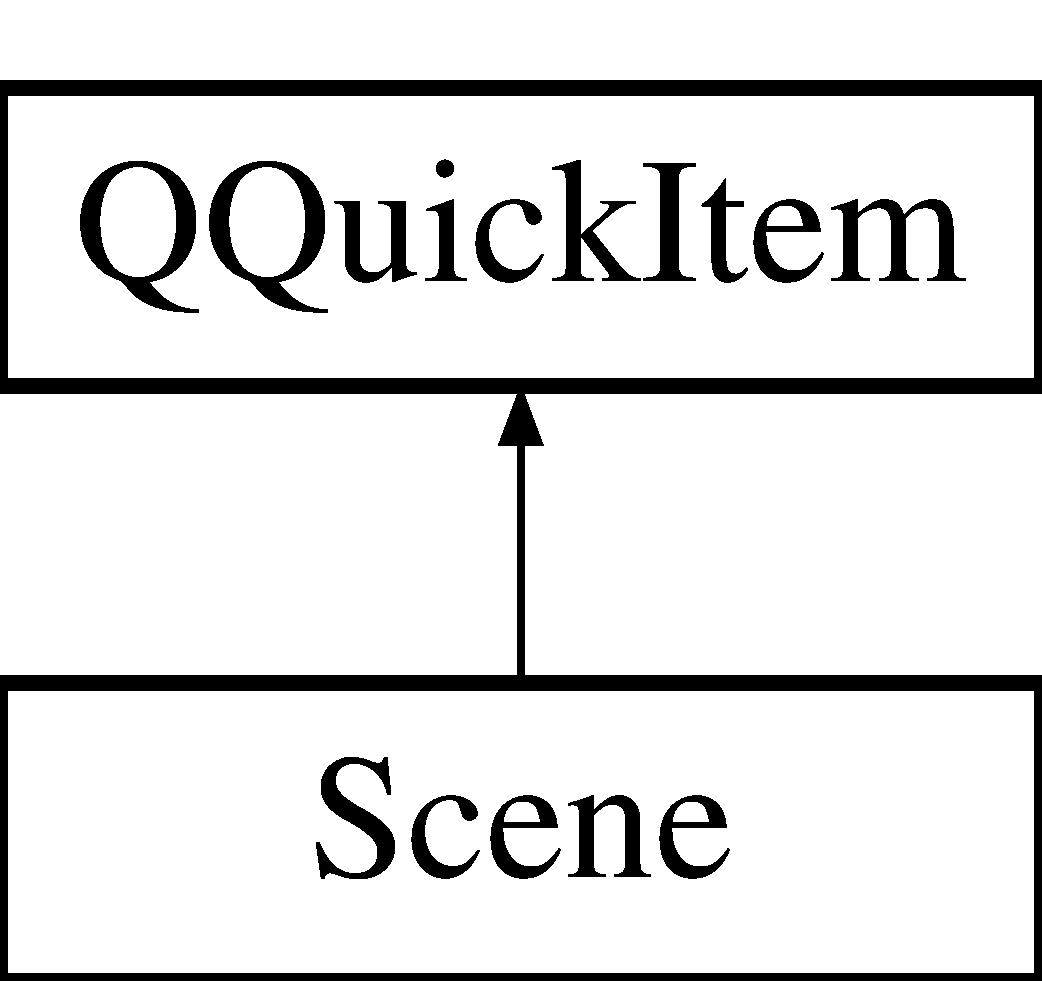
\includegraphics[height=2.000000cm]{class_scene}
\end{center}
\end{figure}
\subsection*{Public Slots}
\begin{DoxyCompactItemize}
\item 
\hypertarget{class_scene_affe50b48f645e09b22f6f8c5c0561654}{}virtual void {\bfseries sync} (int elapsed\+Time)\label{class_scene_affe50b48f645e09b22f6f8c5c0561654}

\item 
\hypertarget{class_scene_abc75a5de4f5a191816e6e1901b7b62bf}{}virtual void {\bfseries cleanup\+G\+L} (Q\+Open\+G\+L\+Functions \&gl)\label{class_scene_abc75a5de4f5a191816e6e1901b7b62bf}

\item 
\hypertarget{class_scene_a0d27204bee9a3211c83bc81f592b5c3c}{}void {\bfseries paint} (Q\+Open\+G\+L\+Functions \&gl, const Q\+Matrix4x4 \&view\+Projection, const Q\+Map$<$ Shader\+Programs, Q\+Open\+G\+L\+Shader\+Program $\ast$ $>$ \&shader\+Programs)\label{class_scene_a0d27204bee9a3211c83bc81f592b5c3c}

\item 
\hypertarget{class_scene_ace3407a4d148d317a20b1bf205554bc5}{}void {\bfseries register\+Navigation} (\hyperlink{class_navigation}{Navigation} $\ast$navigation)\label{class_scene_ace3407a4d148d317a20b1bf205554bc5}

\item 
\hypertarget{class_scene_ade6d7968a2bad7c1dfbae98045a8aa7d}{}void {\bfseries rotate\+Current\+Gem} (const Q\+Quaternion \&quaternion)\label{class_scene_ade6d7968a2bad7c1dfbae98045a8aa7d}

\end{DoxyCompactItemize}
\subsection*{Signals}
\begin{DoxyCompactItemize}
\item 
\hypertarget{class_scene_a9c23e7cda34a3089165ce18c2ec89c15}{}void {\bfseries cubes\+Changed} ()\label{class_scene_a9c23e7cda34a3089165ce18c2ec89c15}

\item 
\hypertarget{class_scene_a8df7e2ef0bf2910fa03df1c16b255551}{}void {\bfseries geometries\+Changed} ()\label{class_scene_a8df7e2ef0bf2910fa03df1c16b255551}

\item 
\hypertarget{class_scene_a4eed91c96f13a7646830737b820755c4}{}void {\bfseries root\+Light\+Ray\+Changed} ()\label{class_scene_a4eed91c96f13a7646830737b820755c4}

\end{DoxyCompactItemize}
\subsection*{Public Member Functions}
\begin{DoxyCompactItemize}
\item 
\hypertarget{class_scene_a93f88c89ce94ad70a668225522818b1e}{}{\bfseries Scene} (Q\+Quick\+Item $\ast$parent=0)\label{class_scene_a93f88c89ce94ad70a668225522818b1e}

\item 
\hypertarget{class_scene_a34966e5d9859ef84b3867b29f26c4dc6}{}Q\+Qml\+List\+Property$<$ \hyperlink{class_abstract_gem}{Abstract\+Gem} $>$ {\bfseries geometries} ()\label{class_scene_a34966e5d9859ef84b3867b29f26c4dc6}

\item 
\hypertarget{class_scene_a81b014ae882dfaec147d917b1ea99d68}{}\hyperlink{class_camera}{Camera} $\ast$ {\bfseries camera} () const \label{class_scene_a81b014ae882dfaec147d917b1ea99d68}

\item 
\hypertarget{class_scene_a4c722c43b266a642a4a06d0d818b14d1}{}void {\bfseries set\+Camera} (\hyperlink{class_camera}{Camera} $\ast$camera)\label{class_scene_a4c722c43b266a642a4a06d0d818b14d1}

\item 
\hypertarget{class_scene_ac8f232cf7cae52e2a235f63589fe85b5}{}\hyperlink{class_scene_renderer}{Scene\+Renderer} \& {\bfseries scene\+Renderer} () const \label{class_scene_ac8f232cf7cae52e2a235f63589fe85b5}

\item 
\hyperlink{class_abstract_gem}{Abstract\+Gem} $\ast$ \hyperlink{class_scene_af96ea722705769055ef2f9e9572f3fa0}{find\+Gem\+With\+Bounding\+Sphere\+Intersected\+By} (const \hyperlink{class_light_ray}{Light\+Ray} \&ray, Q\+Vector3\+D $\ast$collision\+Point=nullptr) const 
\begin{DoxyCompactList}\small\item\em Finds the nearest gem, that bounding sphere is intersected by given ray. \end{DoxyCompactList}\item 
\hyperlink{class_abstract_gem}{Abstract\+Gem} $\ast$ \hyperlink{class_scene_a2a2cee0a97d8436aac1cd582904af459}{find\+Gem\+Intersected\+By} (const \hyperlink{class_light_ray}{Light\+Ray} \&ray, Q\+Vector3\+D $\ast$collision\+Point=nullptr) const 
\begin{DoxyCompactList}\small\item\em Finds the nearest gem with bounding sphere intersected by given ray. \end{DoxyCompactList}\item 
\hyperlink{class_triangle}{Triangle} $\ast$ \hyperlink{class_scene_a2a06baa2386486f9276f97c47d76e624}{find\+Gem\+Face\+Intersected\+By} (const \hyperlink{class_light_ray}{Light\+Ray} \&ray, Q\+Vector3\+D $\ast$collision\+Point=nullptr) const 
\begin{DoxyCompactList}\small\item\em Finds intersected face of nearest gem intersected by given ray. \end{DoxyCompactList}\item 
\hypertarget{class_scene_afcaeead320358b9d9dd02a113ef97c44}{}void {\bfseries set\+Current\+Gem} (\hyperlink{class_abstract_gem}{Abstract\+Gem} $\ast$current\+Gem)\label{class_scene_afcaeead320358b9d9dd02a113ef97c44}

\item 
\hypertarget{class_scene_a7de6dcc38dd6398f71af71295ae09966}{}\hyperlink{class_light_ray}{Light\+Ray} $\ast$ {\bfseries root\+Light\+Ray} () const \label{class_scene_a7de6dcc38dd6398f71af71295ae09966}

\item 
\hypertarget{class_scene_a3da6be3089fe335bf628ef58d23cda18}{}void {\bfseries set\+Root\+Light\+Ray} (\hyperlink{class_light_ray}{Light\+Ray} $\ast$root\+Light\+Ray)\label{class_scene_a3da6be3089fe335bf628ef58d23cda18}

\end{DoxyCompactItemize}
\subsection*{Protected Attributes}
\begin{DoxyCompactItemize}
\item 
\hypertarget{class_scene_a62831eb6a67ce74ee608b4327bf069f3}{}\hyperlink{class_scene_bounds}{Scene\+Bounds} $\ast$ {\bfseries m\+\_\+bounds}\label{class_scene_a62831eb6a67ce74ee608b4327bf069f3}

\item 
\hypertarget{class_scene_ab37f5e133a5fe0803c3df42a4fcba7bf}{}\hyperlink{class_camera}{Camera} $\ast$ {\bfseries m\+\_\+camera}\label{class_scene_ab37f5e133a5fe0803c3df42a4fcba7bf}

\item 
\hypertarget{class_scene_aff9d5a2212ba1b5813dc10177f0344cb}{}\hyperlink{class_abstract_gem}{Abstract\+Gem} $\ast$ {\bfseries m\+\_\+current\+Gem}\label{class_scene_aff9d5a2212ba1b5813dc10177f0344cb}

\item 
\hypertarget{class_scene_a4865a91dd0d6d9af51a7e5cb74d9c991}{}\hyperlink{class_q_list}{Q\+List}$<$ \hyperlink{class_abstract_gem}{Abstract\+Gem} $\ast$ $>$ {\bfseries m\+\_\+gem}\label{class_scene_a4865a91dd0d6d9af51a7e5cb74d9c991}

\item 
\hypertarget{class_scene_ab06de12f271bb51852aedf06285b1032}{}\hyperlink{class_light_ray_renderer}{Light\+Ray\+Renderer} $\ast$ {\bfseries m\+\_\+light\+Ray\+Renderer}\label{class_scene_ab06de12f271bb51852aedf06285b1032}

\item 
\hypertarget{class_scene_a595ab554271bd87c4c73f0cce175ff81}{}\hyperlink{class_navigation}{Navigation} $\ast$ {\bfseries m\+\_\+navigation}\label{class_scene_a595ab554271bd87c4c73f0cce175ff81}

\item 
\hypertarget{class_scene_aa7040eec94173f3ca255a35f926fad6f}{}\hyperlink{class_scene_renderer}{Scene\+Renderer} $\ast$ {\bfseries m\+\_\+renderer}\label{class_scene_aa7040eec94173f3ca255a35f926fad6f}

\item 
\hypertarget{class_scene_a766daf7b6a92c877f1fc57f3d8af9959}{}\hyperlink{class_light_ray}{Light\+Ray} $\ast$ {\bfseries m\+\_\+root\+Light\+Ray}\label{class_scene_a766daf7b6a92c877f1fc57f3d8af9959}

\end{DoxyCompactItemize}
\subsection*{Properties}
\begin{DoxyCompactItemize}
\item 
\hypertarget{class_scene_a827a20f41fe948e08f2774579b91d048}{}Q\+Qml\+List\+Property$<$ \hyperlink{class_abstract_gem}{Abstract\+Gem} $>$ {\bfseries geometries}\label{class_scene_a827a20f41fe948e08f2774579b91d048}

\item 
\hypertarget{class_scene_ab915c54546b8cecc3ae6bb7c8983518c}{}\hyperlink{class_camera}{Camera} {\bfseries camera}\label{class_scene_ab915c54546b8cecc3ae6bb7c8983518c}

\item 
\hypertarget{class_scene_a437a4ce938a6de368c2a6abba0ec3f3d}{}\hyperlink{class_light_ray}{Light\+Ray} {\bfseries root\+Light\+Ray}\label{class_scene_a437a4ce938a6de368c2a6abba0ec3f3d}

\end{DoxyCompactItemize}


\subsection{Member Function Documentation}
\hypertarget{class_scene_a2a06baa2386486f9276f97c47d76e624}{}\index{Scene@{Scene}!find\+Gem\+Face\+Intersected\+By@{find\+Gem\+Face\+Intersected\+By}}
\index{find\+Gem\+Face\+Intersected\+By@{find\+Gem\+Face\+Intersected\+By}!Scene@{Scene}}
\subsubsection[{find\+Gem\+Face\+Intersected\+By}]{\setlength{\rightskip}{0pt plus 5cm}{\bf Triangle} $\ast$ Scene\+::find\+Gem\+Face\+Intersected\+By (
\begin{DoxyParamCaption}
\item[{const {\bf Light\+Ray} \&}]{ray, }
\item[{Q\+Vector3\+D $\ast$}]{collision\+Point = {\ttfamily nullptr}}
\end{DoxyParamCaption}
) const}\label{class_scene_a2a06baa2386486f9276f97c47d76e624}


Finds intersected face of nearest gem intersected by given ray. 


\begin{DoxyParams}{Parameters}
{\em ray} & Ray send into scene to find gem face. \\
\hline
{\em collision\+Point} & Optional parameter. The point of collision is written into. Only if no nullptr is returned this value is useable. \\
\hline
\end{DoxyParams}
\begin{DoxyReturn}{Returns}
Returns the nearst intersected face of a gem. Returns never nullptr. 
\end{DoxyReturn}
\hypertarget{class_scene_a2a2cee0a97d8436aac1cd582904af459}{}\index{Scene@{Scene}!find\+Gem\+Intersected\+By@{find\+Gem\+Intersected\+By}}
\index{find\+Gem\+Intersected\+By@{find\+Gem\+Intersected\+By}!Scene@{Scene}}
\subsubsection[{find\+Gem\+Intersected\+By}]{\setlength{\rightskip}{0pt plus 5cm}{\bf Abstract\+Gem} $\ast$ Scene\+::find\+Gem\+Intersected\+By (
\begin{DoxyParamCaption}
\item[{const {\bf Light\+Ray} \&}]{ray, }
\item[{Q\+Vector3\+D $\ast$}]{collision\+Point = {\ttfamily nullptr}}
\end{DoxyParamCaption}
) const}\label{class_scene_a2a2cee0a97d8436aac1cd582904af459}


Finds the nearest gem with bounding sphere intersected by given ray. 


\begin{DoxyParams}{Parameters}
{\em ray} & Ray send into scene to find gem. \\
\hline
{\em collision\+Point} & Optional parameter. The point of collision is written into. \\
\hline
\end{DoxyParams}
\begin{DoxyReturn}{Returns}
Returns the nearst intersected gem. Returns never a nullptr; 
\end{DoxyReturn}
\hypertarget{class_scene_af96ea722705769055ef2f9e9572f3fa0}{}\index{Scene@{Scene}!find\+Gem\+With\+Bounding\+Sphere\+Intersected\+By@{find\+Gem\+With\+Bounding\+Sphere\+Intersected\+By}}
\index{find\+Gem\+With\+Bounding\+Sphere\+Intersected\+By@{find\+Gem\+With\+Bounding\+Sphere\+Intersected\+By}!Scene@{Scene}}
\subsubsection[{find\+Gem\+With\+Bounding\+Sphere\+Intersected\+By}]{\setlength{\rightskip}{0pt plus 5cm}{\bf Abstract\+Gem} $\ast$ Scene\+::find\+Gem\+With\+Bounding\+Sphere\+Intersected\+By (
\begin{DoxyParamCaption}
\item[{const {\bf Light\+Ray} \&}]{ray, }
\item[{Q\+Vector3\+D $\ast$}]{collision\+Point = {\ttfamily nullptr}}
\end{DoxyParamCaption}
) const}\label{class_scene_af96ea722705769055ef2f9e9572f3fa0}


Finds the nearest gem, that bounding sphere is intersected by given ray. 


\begin{DoxyParams}{Parameters}
{\em ray} & Ray send into scene to find gem. \\
\hline
{\em collision\+Point} & Optional parameter. The point of collision is written into. Only if no nullptr is returned this value is useable. \\
\hline
\end{DoxyParams}
\begin{DoxyReturn}{Returns}
Returns the nearst intersected gem. Returns never nullptr. 
\end{DoxyReturn}


The documentation for this class was generated from the following files\+:\begin{DoxyCompactItemize}
\item 
gem\+Illuminator/scene.\+h\item 
gem\+Illuminator/scene.\+cpp\end{DoxyCompactItemize}

\hypertarget{class_scene_bounds}{\section{Scene\+Bounds Class Reference}
\label{class_scene_bounds}\index{Scene\+Bounds@{Scene\+Bounds}}
}


The \hyperlink{class_scene_bounds}{Scene\+Bounds} class is a special kind of gem describing the bounds of scene. The shape of the bounds is a cube, with a given extent in each direction.  The main reason that the bounds are also a gem is easier collision detection. If we have bounds around our scene every ray emitted into scene will hit something. Furthermore the collision with scene bounds can be processed in a way, that the player will lose if the player hits the bounds.  




{\ttfamily \#include $<$scenebounds.\+h$>$}

Inheritance diagram for Scene\+Bounds\+:\begin{figure}[H]
\begin{center}
\leavevmode
\includegraphics[height=3.000000cm]{class_scene_bounds}
\end{center}
\end{figure}
\subsection*{Public Member Functions}
\begin{DoxyCompactItemize}
\item 
\hyperlink{class_scene_bounds_a26e24012c6a45d3412745828b037dae4}{Scene\+Bounds} (Q\+Object $\ast$parent=0)
\begin{DoxyCompactList}\small\item\em Creates new \hyperlink{class_scene_bounds}{Scene\+Bounds}. The extent of bounds is taken from config file. \end{DoxyCompactList}\item 
virtual \hyperlink{class_scene_bounds_a625ef0d42c9133022a636ba5a57ad840}{$\sim$\+Scene\+Bounds} ()
\item 
void \hyperlink{class_scene_bounds_a26db5e7928d3ac7d0257dc52e1ed4e77}{set\+Position} (const Q\+Vector3\+D \&position) override
\begin{DoxyCompactList}\small\item\em Override \hyperlink{class_abstract_gem_aaf11fa4b522dc334ebed4f2d031a3e2b}{Abstract\+Gem\+::set\+Position()} in order to forbid moving the bounds around. \end{DoxyCompactList}\item 
void \hyperlink{class_scene_bounds_a2e7b2f2e66700b414584ca6b407faf72}{set\+Rotation} (const Q\+Quaternion \&rotation) override
\begin{DoxyCompactList}\small\item\em set\+Rotation Override \hyperlink{class_abstract_gem_afce4d09f74fec117d27b11a220eee6b9}{Abstract\+Gem\+::set\+Rotation()} in order to forbid rotating the bounds. \end{DoxyCompactList}\item 
\hyperlink{singleton_q_list}{Q\+List}$<$ \hyperlink{class_light_ray}{Light\+Ray} $\ast$ $>$ \hyperlink{class_scene_bounds_aeac6aafe6081e8efd6b4180e86346dc0}{process\+Ray\+Intersection} (const \hyperlink{class_light_ray}{Light\+Ray} \&ray, \hyperlink{class_scene}{Scene} $\ast$scene) override
\begin{DoxyCompactList}\small\item\em Override \hyperlink{class_abstract_gem_ab4f3c6d38acbe59a610c67588e4944d7}{Abstract\+Gem\+::process\+Ray\+Intersection()} in order to ensure the player loses hitting the bounds. \end{DoxyCompactList}\end{DoxyCompactItemize}
\subsection*{Additional Inherited Members}


\subsection{Detailed Description}
The \hyperlink{class_scene_bounds}{Scene\+Bounds} class is a special kind of gem describing the bounds of scene. The shape of the bounds is a cube, with a given extent in each direction.  The main reason that the bounds are also a gem is easier collision detection. If we have bounds around our scene every ray emitted into scene will hit something. Furthermore the collision with scene bounds can be processed in a way, that the player will lose if the player hits the bounds. 

\subsection{Constructor \& Destructor Documentation}
\hypertarget{class_scene_bounds_a26e24012c6a45d3412745828b037dae4}{\index{Scene\+Bounds@{Scene\+Bounds}!Scene\+Bounds@{Scene\+Bounds}}
\index{Scene\+Bounds@{Scene\+Bounds}!Scene\+Bounds@{Scene\+Bounds}}
\subsubsection[{Scene\+Bounds}]{\setlength{\rightskip}{0pt plus 5cm}Scene\+Bounds\+::\+Scene\+Bounds (
\begin{DoxyParamCaption}
\item[{Q\+Object $\ast$}]{parent = {\ttfamily 0}}
\end{DoxyParamCaption}
)\hspace{0.3cm}{\ttfamily [explicit]}}}\label{class_scene_bounds_a26e24012c6a45d3412745828b037dae4}


Creates new \hyperlink{class_scene_bounds}{Scene\+Bounds}. The extent of bounds is taken from config file. 


\begin{DoxyParams}{Parameters}
{\em parent} & \\
\hline
\end{DoxyParams}
\hypertarget{class_scene_bounds_a625ef0d42c9133022a636ba5a57ad840}{\index{Scene\+Bounds@{Scene\+Bounds}!````~Scene\+Bounds@{$\sim$\+Scene\+Bounds}}
\index{````~Scene\+Bounds@{$\sim$\+Scene\+Bounds}!Scene\+Bounds@{Scene\+Bounds}}
\subsubsection[{$\sim$\+Scene\+Bounds}]{\setlength{\rightskip}{0pt plus 5cm}Scene\+Bounds\+::$\sim$\+Scene\+Bounds (
\begin{DoxyParamCaption}
{}
\end{DoxyParamCaption}
)\hspace{0.3cm}{\ttfamily [virtual]}}}\label{class_scene_bounds_a625ef0d42c9133022a636ba5a57ad840}


\subsection{Member Function Documentation}
\hypertarget{class_scene_bounds_aeac6aafe6081e8efd6b4180e86346dc0}{\index{Scene\+Bounds@{Scene\+Bounds}!process\+Ray\+Intersection@{process\+Ray\+Intersection}}
\index{process\+Ray\+Intersection@{process\+Ray\+Intersection}!Scene\+Bounds@{Scene\+Bounds}}
\subsubsection[{process\+Ray\+Intersection}]{\setlength{\rightskip}{0pt plus 5cm}{\bf Q\+List}$<$ {\bf Light\+Ray} $\ast$ $>$ Scene\+Bounds\+::process\+Ray\+Intersection (
\begin{DoxyParamCaption}
\item[{const {\bf Light\+Ray} \&}]{ray, }
\item[{{\bf Scene} $\ast$}]{scene}
\end{DoxyParamCaption}
)\hspace{0.3cm}{\ttfamily [override]}, {\ttfamily [virtual]}}}\label{class_scene_bounds_aeac6aafe6081e8efd6b4180e86346dc0}


Override \hyperlink{class_abstract_gem_ab4f3c6d38acbe59a610c67588e4944d7}{Abstract\+Gem\+::process\+Ray\+Intersection()} in order to ensure the player loses hitting the bounds. 


\begin{DoxyParams}{Parameters}
{\em ray} & The ray hitting the bounds. \\
\hline
{\em scene} & The scene containing all lightrays. \\
\hline
\end{DoxyParams}
\begin{DoxyReturn}{Returns}
Returns a \hyperlink{singleton_q_list}{Q\+List} containing only a \hyperlink{class_game_lost_ray}{Game\+Lost\+Ray}, so the player will loose as soon as the player tries to move on returned ray. 
\end{DoxyReturn}


Reimplemented from \hyperlink{class_abstract_gem_ab4f3c6d38acbe59a610c67588e4944d7}{Abstract\+Gem}.

\hypertarget{class_scene_bounds_a26db5e7928d3ac7d0257dc52e1ed4e77}{\index{Scene\+Bounds@{Scene\+Bounds}!set\+Position@{set\+Position}}
\index{set\+Position@{set\+Position}!Scene\+Bounds@{Scene\+Bounds}}
\subsubsection[{set\+Position}]{\setlength{\rightskip}{0pt plus 5cm}void Scene\+Bounds\+::set\+Position (
\begin{DoxyParamCaption}
\item[{const Q\+Vector3\+D \&}]{position}
\end{DoxyParamCaption}
)\hspace{0.3cm}{\ttfamily [override]}, {\ttfamily [virtual]}}}\label{class_scene_bounds_a26db5e7928d3ac7d0257dc52e1ed4e77}


Override \hyperlink{class_abstract_gem_aaf11fa4b522dc334ebed4f2d031a3e2b}{Abstract\+Gem\+::set\+Position()} in order to forbid moving the bounds around. 


\begin{DoxyParams}{Parameters}
{\em position} & This parameter will be ignored. \\
\hline
\end{DoxyParams}


Reimplemented from \hyperlink{class_abstract_gem_aaf11fa4b522dc334ebed4f2d031a3e2b}{Abstract\+Gem}.

\hypertarget{class_scene_bounds_a2e7b2f2e66700b414584ca6b407faf72}{\index{Scene\+Bounds@{Scene\+Bounds}!set\+Rotation@{set\+Rotation}}
\index{set\+Rotation@{set\+Rotation}!Scene\+Bounds@{Scene\+Bounds}}
\subsubsection[{set\+Rotation}]{\setlength{\rightskip}{0pt plus 5cm}void Scene\+Bounds\+::set\+Rotation (
\begin{DoxyParamCaption}
\item[{const Q\+Quaternion \&}]{rotation}
\end{DoxyParamCaption}
)\hspace{0.3cm}{\ttfamily [override]}, {\ttfamily [virtual]}}}\label{class_scene_bounds_a2e7b2f2e66700b414584ca6b407faf72}


set\+Rotation Override \hyperlink{class_abstract_gem_afce4d09f74fec117d27b11a220eee6b9}{Abstract\+Gem\+::set\+Rotation()} in order to forbid rotating the bounds. 


\begin{DoxyParams}{Parameters}
{\em rotation} & This parameter will be ignored. \\
\hline
\end{DoxyParams}


Reimplemented from \hyperlink{class_abstract_gem_afce4d09f74fec117d27b11a220eee6b9}{Abstract\+Gem}.



The documentation for this class was generated from the following files\+:\begin{DoxyCompactItemize}
\item 
\hyperlink{scenebounds_8h}{scenebounds.\+h}\item 
\hyperlink{scenebounds_8cpp}{scenebounds.\+cpp}\end{DoxyCompactItemize}

\hypertarget{class_scene_renderer}{}\section{Scene\+Renderer Class Reference}
\label{class_scene_renderer}\index{Scene\+Renderer@{Scene\+Renderer}}


The \hyperlink{class_scene_renderer}{Scene\+Renderer} class  Renders the scene\+: Packs the scene in the buffer and draws the scene in one call.  




{\ttfamily \#include $<$scenerenderer.\+h$>$}

Inheritance diagram for Scene\+Renderer\+:\begin{figure}[H]
\begin{center}
\leavevmode
\includegraphics[height=2.000000cm]{class_scene_renderer}
\end{center}
\end{figure}
\subsection*{Public Slots}
\begin{DoxyCompactItemize}
\item 
\hypertarget{class_scene_renderer_a0b6e4d40b218acb45ea13bb4fda494e5}{}void {\bfseries paint} (Q\+Open\+G\+L\+Functions \&gl, const Q\+Matrix4x4 \&view\+Projection, const Q\+Map$<$ Shader\+Programs, Q\+Open\+G\+L\+Shader\+Program $\ast$ $>$ \&shader\+Programs)\label{class_scene_renderer_a0b6e4d40b218acb45ea13bb4fda494e5}

\end{DoxyCompactItemize}
\subsection*{Public Member Functions}
\begin{DoxyCompactItemize}
\item 
\hypertarget{class_scene_renderer_a12f72dc9b22e99ecdccaec38b6d2d512}{}{\bfseries Scene\+Renderer} (Q\+Object $\ast$parent=0)\label{class_scene_renderer_a12f72dc9b22e99ecdccaec38b6d2d512}

\item 
\hypertarget{class_scene_renderer_a9dc118d75160651fb925410a68fef70f}{}void {\bfseries cleanup} (Q\+Open\+G\+L\+Functions \&gl)\label{class_scene_renderer_a9dc118d75160651fb925410a68fef70f}

\item 
\hypertarget{class_scene_renderer_a0cae4e7fdd5ef1fd4d38f480521433a9}{}void {\bfseries synchronize\+Geometries} (\hyperlink{class_q_list}{Q\+List}$<$ \hyperlink{class_abstract_gem}{Abstract\+Gem} $\ast$ $>$ geometries)\label{class_scene_renderer_a0cae4e7fdd5ef1fd4d38f480521433a9}

\item 
\hypertarget{class_scene_renderer_a6596dcdb04a471f4fbcfa82eed07b9d8}{}void {\bfseries set\+Scene\+Extent} (float extent)\label{class_scene_renderer_a6596dcdb04a471f4fbcfa82eed07b9d8}

\item 
\hypertarget{class_scene_renderer_ad57b11f56edc29b4e46a9104af6efe6d}{}\hyperlink{class_light_ray}{Light\+Ray} $\ast$ {\bfseries root\+Light\+Ray} () const \label{class_scene_renderer_ad57b11f56edc29b4e46a9104af6efe6d}

\item 
\hypertarget{class_scene_renderer_a8e9b701f5b236adbe805715944d9ae8c}{}void {\bfseries set\+Root\+Light\+Ray} (\hyperlink{class_light_ray}{Light\+Ray} $\ast$root\+Light\+Ray)\label{class_scene_renderer_a8e9b701f5b236adbe805715944d9ae8c}

\end{DoxyCompactItemize}
\subsection*{Protected Member Functions}
\begin{DoxyCompactItemize}
\item 
\hypertarget{class_scene_renderer_a6a8fecf9dcfcda180e4f9d2abb0ca2e8}{}void {\bfseries paint\+Gems} (Q\+Open\+G\+L\+Functions \&gl, const Q\+Matrix4x4 \&view\+Projection, Q\+Open\+G\+L\+Shader\+Program \&shader\+Program)\label{class_scene_renderer_a6a8fecf9dcfcda180e4f9d2abb0ca2e8}

\item 
\hypertarget{class_scene_renderer_a6371e0e5c63e519fcf407f12d9d47262}{}void {\bfseries paint\+Light\+Rays} (Q\+Open\+G\+L\+Functions \&gl, const Q\+Matrix4x4 \&view\+Projection, Q\+Open\+G\+L\+Shader\+Program \&shader\+Program)\label{class_scene_renderer_a6371e0e5c63e519fcf407f12d9d47262}

\end{DoxyCompactItemize}
\subsection*{Protected Attributes}
\begin{DoxyCompactItemize}
\item 
\hypertarget{class_scene_renderer_adf73dd839ccd615bf377b8dba695255e}{}\hyperlink{class_gem_renderer}{Gem\+Renderer} $\ast$ {\bfseries m\+\_\+gem\+Renderer}\label{class_scene_renderer_adf73dd839ccd615bf377b8dba695255e}

\item 
\hypertarget{class_scene_renderer_af2d4ded15e32fd485295fc0531645dc1}{}\hyperlink{class_q_list}{Q\+List}$<$ \hyperlink{class_abstract_gem}{Abstract\+Gem} $\ast$ $>$ {\bfseries m\+\_\+geometries}\label{class_scene_renderer_af2d4ded15e32fd485295fc0531645dc1}

\item 
\hypertarget{class_scene_renderer_aec10558966df8efad69726e9b06d0cfd}{}\hyperlink{class_light_ray}{Light\+Ray} $\ast$ {\bfseries m\+\_\+root\+Light\+Ray}\label{class_scene_renderer_aec10558966df8efad69726e9b06d0cfd}

\item 
\hypertarget{class_scene_renderer_ae9cdbec278ec42dac41c7f1d9d75388f}{}float {\bfseries m\+\_\+scene\+Extent}\label{class_scene_renderer_ae9cdbec278ec42dac41c7f1d9d75388f}

\end{DoxyCompactItemize}


\subsection{Detailed Description}
The \hyperlink{class_scene_renderer}{Scene\+Renderer} class  Renders the scene\+: Packs the scene in the buffer and draws the scene in one call. 

The documentation for this class was generated from the following files\+:\begin{DoxyCompactItemize}
\item 
gem\+Illuminator/scenerenderer.\+h\item 
gem\+Illuminator/scenerenderer.\+cpp\end{DoxyCompactItemize}

\hypertarget{class_screen_aligned_quad}{}\section{Screen\+Aligned\+Quad Class Reference}
\label{class_screen_aligned_quad}\index{Screen\+Aligned\+Quad@{Screen\+Aligned\+Quad}}
\subsection*{Public Member Functions}
\begin{DoxyCompactItemize}
\item 
\hypertarget{class_screen_aligned_quad_ac288d2712b9846afb5077af53b454761}{}void {\bfseries draw} (Q\+Open\+G\+L\+Functions \&gl)\label{class_screen_aligned_quad_ac288d2712b9846afb5077af53b454761}

\end{DoxyCompactItemize}
\subsection*{Static Protected Member Functions}
\begin{DoxyCompactItemize}
\item 
\hypertarget{class_screen_aligned_quad_a103c649c457d5fcaf90d3f8ed4b7e208}{}static void {\bfseries strip} (Q\+Open\+G\+L\+Buffer \&vertices)\label{class_screen_aligned_quad_a103c649c457d5fcaf90d3f8ed4b7e208}

\end{DoxyCompactItemize}


The documentation for this class was generated from the following files\+:\begin{DoxyCompactItemize}
\item 
gem\+Illuminator/screenalignedquad.\+h\item 
gem\+Illuminator/screenalignedquad.\+cpp\end{DoxyCompactItemize}

\hypertarget{class_soundmanager}{}\section{Soundmanager Class Reference}
\label{class_soundmanager}\index{Soundmanager@{Soundmanager}}


The \hyperlink{class_soundmanager}{Soundmanager} class provides several sounds which can be played.  The \hyperlink{class_soundmanager}{Soundmanager} manages the required ressources.  




{\ttfamily \#include $<$soundmanager.\+h$>$}

Inheritance diagram for Soundmanager\+:\begin{figure}[H]
\begin{center}
\leavevmode
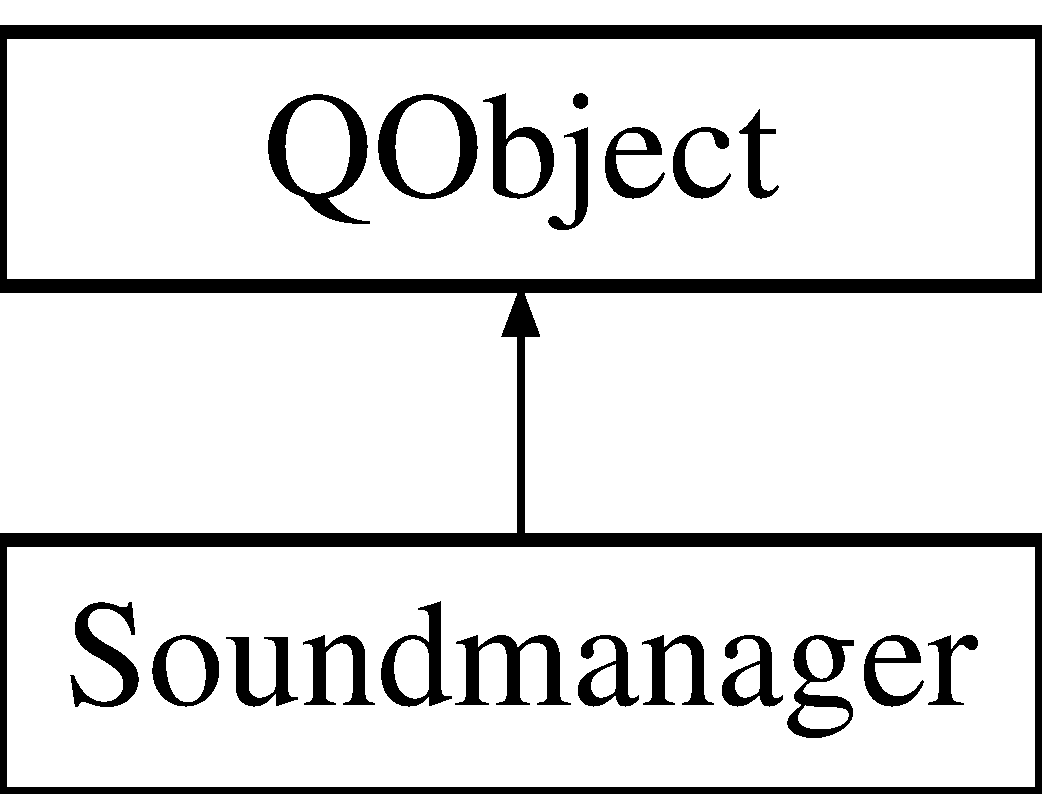
\includegraphics[height=2.000000cm]{class_soundmanager}
\end{center}
\end{figure}
\subsection*{Public Member Functions}
\begin{DoxyCompactItemize}
\item 
virtual \hyperlink{class_soundmanager_a098a604a4cb0a238863ddb0065f11885}{$\sim$\+Soundmanager} ()
\item 
Q\+\_\+\+I\+N\+V\+O\+K\+A\+B\+L\+E void \hyperlink{class_soundmanager_adc77c21e0705c9220b6bfff6d8957d7c}{play\+Background\+Music} ()
\begin{DoxyCompactList}\small\item\em Starts playing our background music. \end{DoxyCompactList}\item 
void \hyperlink{class_soundmanager_a6116af7088ee72cafda5d3e1c6b6600b}{play\+Collision\+Sound} ()
\begin{DoxyCompactList}\small\item\em Plays a previously defined sound in order to indicate a collision. \end{DoxyCompactList}\item 
void \hyperlink{class_soundmanager_a490ddb5b63b94701ad5d246d27759b14}{set\+Collision\+Sound} (\hyperlink{soundmanager_8h_a7fbdfef23a43c911ebc18ef1b9d9808d}{Sound\+Effects} effect)
\begin{DoxyCompactList}\small\item\em Sets the collision sound that will be played next time \hyperlink{class_soundmanager_a6116af7088ee72cafda5d3e1c6b6600b}{play\+Collision\+Sound()} is called. \end{DoxyCompactList}\item 
Q\+\_\+\+I\+N\+V\+O\+K\+A\+B\+L\+E void \hyperlink{class_soundmanager_a36411846ae8c5cd18239cfb913f3dc83}{stop\+Background\+Music} ()
\begin{DoxyCompactList}\small\item\em Stops playing our background music. \end{DoxyCompactList}\end{DoxyCompactItemize}
\subsection*{Static Public Member Functions}
\begin{DoxyCompactItemize}
\item 
static void \hyperlink{class_soundmanager_aa4a2f89d1c517bff42654038da492d65}{drop} ()
\begin{DoxyCompactList}\small\item\em Drops current instance of our \hyperlink{class_soundmanager}{Soundmanager}. \end{DoxyCompactList}\item 
static \hyperlink{class_soundmanager}{Soundmanager} $\ast$ \hyperlink{class_soundmanager_aa1fa87053cd1cd240447a54327962b23}{instance} ()
\begin{DoxyCompactList}\small\item\em The instance of our \hyperlink{class_soundmanager}{Soundmanager}. \end{DoxyCompactList}\end{DoxyCompactItemize}
\subsection*{Protected Member Functions}
\begin{DoxyCompactItemize}
\item 
\hyperlink{class_soundmanager_a8b484955e5732155f07099e53dca61e1}{Soundmanager} ()
\item 
void \hyperlink{class_soundmanager_a97874137f1bc5dcff106b0a5faeca828}{load\+Sounds} ()
\end{DoxyCompactItemize}
\subsection*{Protected Attributes}
\begin{DoxyCompactItemize}
\item 
Q\+Media\+Player $\ast$ \hyperlink{class_soundmanager_a39e32f7d94670486c52e78721a8f4faf}{m\+\_\+background\+Music}
\item 
Q\+Media\+Player $\ast$ \hyperlink{class_soundmanager_a824f9bfdbe61a7db3cb54cb87cb80268}{m\+\_\+collision\+Sound}
\end{DoxyCompactItemize}
\subsection*{Static Protected Attributes}
\begin{DoxyCompactItemize}
\item 
static \hyperlink{class_soundmanager}{Soundmanager} $\ast$ \hyperlink{class_soundmanager_a81105bb352bada9ff056335df0dd2bb3}{m\+\_\+instance} = 0
\end{DoxyCompactItemize}


\subsection{Detailed Description}
The \hyperlink{class_soundmanager}{Soundmanager} class provides several sounds which can be played.  The \hyperlink{class_soundmanager}{Soundmanager} manages the required ressources. 

\subsection{Constructor \& Destructor Documentation}
\hypertarget{class_soundmanager_a098a604a4cb0a238863ddb0065f11885}{}\index{Soundmanager@{Soundmanager}!````~Soundmanager@{$\sim$\+Soundmanager}}
\index{````~Soundmanager@{$\sim$\+Soundmanager}!Soundmanager@{Soundmanager}}
\subsubsection[{$\sim$\+Soundmanager}]{\setlength{\rightskip}{0pt plus 5cm}Soundmanager\+::$\sim$\+Soundmanager (
\begin{DoxyParamCaption}
{}
\end{DoxyParamCaption}
)\hspace{0.3cm}{\ttfamily [virtual]}}\label{class_soundmanager_a098a604a4cb0a238863ddb0065f11885}
\hypertarget{class_soundmanager_a8b484955e5732155f07099e53dca61e1}{}\index{Soundmanager@{Soundmanager}!Soundmanager@{Soundmanager}}
\index{Soundmanager@{Soundmanager}!Soundmanager@{Soundmanager}}
\subsubsection[{Soundmanager}]{\setlength{\rightskip}{0pt plus 5cm}Soundmanager\+::\+Soundmanager (
\begin{DoxyParamCaption}
{}
\end{DoxyParamCaption}
)\hspace{0.3cm}{\ttfamily [protected]}}\label{class_soundmanager_a8b484955e5732155f07099e53dca61e1}


\subsection{Member Function Documentation}
\hypertarget{class_soundmanager_aa4a2f89d1c517bff42654038da492d65}{}\index{Soundmanager@{Soundmanager}!drop@{drop}}
\index{drop@{drop}!Soundmanager@{Soundmanager}}
\subsubsection[{drop}]{\setlength{\rightskip}{0pt plus 5cm}void Soundmanager\+::drop (
\begin{DoxyParamCaption}
{}
\end{DoxyParamCaption}
)\hspace{0.3cm}{\ttfamily [static]}}\label{class_soundmanager_aa4a2f89d1c517bff42654038da492d65}


Drops current instance of our \hyperlink{class_soundmanager}{Soundmanager}. 

\hypertarget{class_soundmanager_aa1fa87053cd1cd240447a54327962b23}{}\index{Soundmanager@{Soundmanager}!instance@{instance}}
\index{instance@{instance}!Soundmanager@{Soundmanager}}
\subsubsection[{instance}]{\setlength{\rightskip}{0pt plus 5cm}{\bf Soundmanager} $\ast$ Soundmanager\+::instance (
\begin{DoxyParamCaption}
{}
\end{DoxyParamCaption}
)\hspace{0.3cm}{\ttfamily [static]}}\label{class_soundmanager_aa1fa87053cd1cd240447a54327962b23}


The instance of our \hyperlink{class_soundmanager}{Soundmanager}. 

\begin{DoxyReturn}{Returns}

\end{DoxyReturn}
\hypertarget{class_soundmanager_a97874137f1bc5dcff106b0a5faeca828}{}\index{Soundmanager@{Soundmanager}!load\+Sounds@{load\+Sounds}}
\index{load\+Sounds@{load\+Sounds}!Soundmanager@{Soundmanager}}
\subsubsection[{load\+Sounds}]{\setlength{\rightskip}{0pt plus 5cm}void Soundmanager\+::load\+Sounds (
\begin{DoxyParamCaption}
{}
\end{DoxyParamCaption}
)\hspace{0.3cm}{\ttfamily [protected]}}\label{class_soundmanager_a97874137f1bc5dcff106b0a5faeca828}
\hypertarget{class_soundmanager_adc77c21e0705c9220b6bfff6d8957d7c}{}\index{Soundmanager@{Soundmanager}!play\+Background\+Music@{play\+Background\+Music}}
\index{play\+Background\+Music@{play\+Background\+Music}!Soundmanager@{Soundmanager}}
\subsubsection[{play\+Background\+Music}]{\setlength{\rightskip}{0pt plus 5cm}void Soundmanager\+::play\+Background\+Music (
\begin{DoxyParamCaption}
{}
\end{DoxyParamCaption}
)}\label{class_soundmanager_adc77c21e0705c9220b6bfff6d8957d7c}


Starts playing our background music. 

\begin{DoxySeeAlso}{See also}
\hyperlink{class_soundmanager_a36411846ae8c5cd18239cfb913f3dc83}{stop\+Background\+Music()} 
\end{DoxySeeAlso}
\hypertarget{class_soundmanager_a6116af7088ee72cafda5d3e1c6b6600b}{}\index{Soundmanager@{Soundmanager}!play\+Collision\+Sound@{play\+Collision\+Sound}}
\index{play\+Collision\+Sound@{play\+Collision\+Sound}!Soundmanager@{Soundmanager}}
\subsubsection[{play\+Collision\+Sound}]{\setlength{\rightskip}{0pt plus 5cm}void Soundmanager\+::play\+Collision\+Sound (
\begin{DoxyParamCaption}
{}
\end{DoxyParamCaption}
)}\label{class_soundmanager_a6116af7088ee72cafda5d3e1c6b6600b}


Plays a previously defined sound in order to indicate a collision. 

\begin{DoxySeeAlso}{See also}
\hyperlink{class_soundmanager_a490ddb5b63b94701ad5d246d27759b14}{set\+Collision\+Sound()} 
\end{DoxySeeAlso}
\hypertarget{class_soundmanager_a490ddb5b63b94701ad5d246d27759b14}{}\index{Soundmanager@{Soundmanager}!set\+Collision\+Sound@{set\+Collision\+Sound}}
\index{set\+Collision\+Sound@{set\+Collision\+Sound}!Soundmanager@{Soundmanager}}
\subsubsection[{set\+Collision\+Sound}]{\setlength{\rightskip}{0pt plus 5cm}void Soundmanager\+::set\+Collision\+Sound (
\begin{DoxyParamCaption}
\item[{{\bf Sound\+Effects}}]{effect}
\end{DoxyParamCaption}
)}\label{class_soundmanager_a490ddb5b63b94701ad5d246d27759b14}


Sets the collision sound that will be played next time \hyperlink{class_soundmanager_a6116af7088ee72cafda5d3e1c6b6600b}{play\+Collision\+Sound()} is called. 


\begin{DoxyParams}{Parameters}
{\em effect} & The choosen Sound\+Effect \\
\hline
\end{DoxyParams}
\hypertarget{class_soundmanager_a36411846ae8c5cd18239cfb913f3dc83}{}\index{Soundmanager@{Soundmanager}!stop\+Background\+Music@{stop\+Background\+Music}}
\index{stop\+Background\+Music@{stop\+Background\+Music}!Soundmanager@{Soundmanager}}
\subsubsection[{stop\+Background\+Music}]{\setlength{\rightskip}{0pt plus 5cm}void Soundmanager\+::stop\+Background\+Music (
\begin{DoxyParamCaption}
{}
\end{DoxyParamCaption}
)}\label{class_soundmanager_a36411846ae8c5cd18239cfb913f3dc83}


Stops playing our background music. 



\subsection{Member Data Documentation}
\hypertarget{class_soundmanager_a39e32f7d94670486c52e78721a8f4faf}{}\index{Soundmanager@{Soundmanager}!m\+\_\+background\+Music@{m\+\_\+background\+Music}}
\index{m\+\_\+background\+Music@{m\+\_\+background\+Music}!Soundmanager@{Soundmanager}}
\subsubsection[{m\+\_\+background\+Music}]{\setlength{\rightskip}{0pt plus 5cm}Q\+Media\+Player$\ast$ Soundmanager\+::m\+\_\+background\+Music\hspace{0.3cm}{\ttfamily [protected]}}\label{class_soundmanager_a39e32f7d94670486c52e78721a8f4faf}
\hypertarget{class_soundmanager_a824f9bfdbe61a7db3cb54cb87cb80268}{}\index{Soundmanager@{Soundmanager}!m\+\_\+collision\+Sound@{m\+\_\+collision\+Sound}}
\index{m\+\_\+collision\+Sound@{m\+\_\+collision\+Sound}!Soundmanager@{Soundmanager}}
\subsubsection[{m\+\_\+collision\+Sound}]{\setlength{\rightskip}{0pt plus 5cm}Q\+Media\+Player$\ast$ Soundmanager\+::m\+\_\+collision\+Sound\hspace{0.3cm}{\ttfamily [protected]}}\label{class_soundmanager_a824f9bfdbe61a7db3cb54cb87cb80268}
\hypertarget{class_soundmanager_a81105bb352bada9ff056335df0dd2bb3}{}\index{Soundmanager@{Soundmanager}!m\+\_\+instance@{m\+\_\+instance}}
\index{m\+\_\+instance@{m\+\_\+instance}!Soundmanager@{Soundmanager}}
\subsubsection[{m\+\_\+instance}]{\setlength{\rightskip}{0pt plus 5cm}{\bf Soundmanager} $\ast$ Soundmanager\+::m\+\_\+instance = 0\hspace{0.3cm}{\ttfamily [static]}, {\ttfamily [protected]}}\label{class_soundmanager_a81105bb352bada9ff056335df0dd2bb3}


The documentation for this class was generated from the following files\+:\begin{DoxyCompactItemize}
\item 
Game-\/\+Programming-\/\+W\+S2014/gem\+Illuminator/\hyperlink{soundmanager_8h}{soundmanager.\+h}\item 
Game-\/\+Programming-\/\+W\+S2014/gem\+Illuminator/\hyperlink{soundmanager_8cpp}{soundmanager.\+cpp}\end{DoxyCompactItemize}

\hypertarget{class_tetrahedron_gem}{}\section{Tetrahedron\+Gem Class Reference}
\label{class_tetrahedron_gem}\index{Tetrahedron\+Gem@{Tetrahedron\+Gem}}
Inheritance diagram for Tetrahedron\+Gem\+:\begin{figure}[H]
\begin{center}
\leavevmode
\includegraphics[height=3.000000cm]{class_tetrahedron_gem}
\end{center}
\end{figure}
\subsection*{Public Member Functions}
\begin{DoxyCompactItemize}
\item 
\hypertarget{class_tetrahedron_gem_af942fcb0a4da9b3dfcf989931b2bc393}{}{\bfseries Tetrahedron\+Gem} (Q\+Object $\ast$parent=0)\label{class_tetrahedron_gem_af942fcb0a4da9b3dfcf989931b2bc393}

\end{DoxyCompactItemize}
\subsection*{Additional Inherited Members}


The documentation for this class was generated from the following files\+:\begin{DoxyCompactItemize}
\item 
gem\+Illuminator/tetrahedrongem.\+h\item 
gem\+Illuminator/tetrahedrongem.\+cpp\end{DoxyCompactItemize}

\hypertarget{class_triangle}{\section{Triangle Class Reference}
\label{class_triangle}\index{Triangle@{Triangle}}
}


The \hyperlink{class_triangle}{Triangle} class represents a triangle in three dimensional space.  




{\ttfamily \#include $<$triangle.\+h$>$}

\subsection*{Public Member Functions}
\begin{DoxyCompactItemize}
\item 
\hyperlink{class_triangle_aaefe4ed500c07918d30c6f0e286332c5}{Triangle} ()
\begin{DoxyCompactList}\small\item\em Creates a new degenerated \hyperlink{class_triangle}{Triangle}, with all points in (0, 0, 0). \end{DoxyCompactList}\item 
\hyperlink{class_triangle_a89052ece2572bfee5d6ade44b9f5094d}{Triangle} (const Q\+Vector3\+D \&\hyperlink{class_triangle_a430bf0a9d8eaf20ea7bdefcd8082588c}{a}, const Q\+Vector3\+D \&\hyperlink{class_triangle_a8327124c9b9b752be94187c9fbf3f460}{b}, const Q\+Vector3\+D \&\hyperlink{class_triangle_a61f6c0245df276555de6d1b1a98840b8}{c})
\begin{DoxyCompactList}\small\item\em Creates a new \hyperlink{class_triangle}{Triangle}, with specified points. It is expected, that points a, b and c are ordered counter clock wise. \end{DoxyCompactList}\item 
\hyperlink{class_triangle_a889893fe34e2eb7121082b86199d5628}{Triangle} (const \hyperlink{class_triangle}{Triangle} \&triangle)
\begin{DoxyCompactList}\small\item\em Creates a new \hyperlink{class_triangle}{Triangle} with data copied from given triangle. \end{DoxyCompactList}\item 
\hyperlink{class_triangle_a5199760a17454f4dc94c855a57e3a152}{$\sim$\+Triangle} ()
\item 
\hyperlink{class_triangle}{Triangle} \& \hyperlink{class_triangle_aae57b61e09898f54256a83e76acfe502}{operator=} (const \hyperlink{class_triangle}{Triangle} \&triangle)
\item 
const Q\+Vector3\+D \& \hyperlink{class_triangle_a430bf0a9d8eaf20ea7bdefcd8082588c}{a} () const 
\item 
void \hyperlink{class_triangle_a24c012d83d7e6c5d0b27985d8dcb64da}{set\+A} (const Q\+Vector3\+D \&\hyperlink{class_triangle_a430bf0a9d8eaf20ea7bdefcd8082588c}{a})
\item 
const Q\+Vector3\+D \& \hyperlink{class_triangle_a8327124c9b9b752be94187c9fbf3f460}{b} () const 
\item 
void \hyperlink{class_triangle_a9f889b49a5ea3b4be4c4366c63673095}{set\+B} (const Q\+Vector3\+D \&\hyperlink{class_triangle_a8327124c9b9b752be94187c9fbf3f460}{b})
\item 
const Q\+Vector3\+D \& \hyperlink{class_triangle_a61f6c0245df276555de6d1b1a98840b8}{c} () const 
\item 
void \hyperlink{class_triangle_af4566995b306c0f9ae72b457b7acb983}{set\+C} (const Q\+Vector3\+D \&\hyperlink{class_triangle_a61f6c0245df276555de6d1b1a98840b8}{c})
\item 
const Q\+Vector3\+D \& \hyperlink{class_triangle_aa1ccf6af0c2567e53b9dc6f51243f934}{normal} () const 
\begin{DoxyCompactList}\small\item\em Returns normal of triangle. The vertices \hyperlink{class_triangle_a430bf0a9d8eaf20ea7bdefcd8082588c}{a()}, \hyperlink{class_triangle_a8327124c9b9b752be94187c9fbf3f460}{b()} and \hyperlink{class_triangle_a61f6c0245df276555de6d1b1a98840b8}{c()} ordered counter clockwise are expected to describe outer side of triangle. \end{DoxyCompactList}\item 
\hyperlink{singleton_q_list}{Q\+List}$<$ Q\+Vector3\+D $>$ \hyperlink{class_triangle_a66da12d2c747c435ea5148df472d9229}{vertices} () const 
\begin{DoxyCompactList}\small\item\em Convenience method. All vertices are returned in \hyperlink{singleton_q_list}{Q\+List}. \end{DoxyCompactList}\item 
Q\+Vector3\+D \hyperlink{class_triangle_a4fb81ac7e355c97a03f4c056bd79ac99}{reflect} (const Q\+Vector3\+D \&incident\+Vector) const 
\begin{DoxyCompactList}\small\item\em Reflects incoming ray at outer side of triangle. \end{DoxyCompactList}\end{DoxyCompactItemize}
\subsection*{Protected Member Functions}
\begin{DoxyCompactItemize}
\item 
void \hyperlink{class_triangle_a429f86c999f5c27720f7b912fa3b20ca}{calculate\+Normal} () const 
\end{DoxyCompactItemize}
\subsection*{Protected Attributes}
\begin{DoxyCompactItemize}
\item 
Q\+Vector3\+D $\ast$ \hyperlink{class_triangle_a38f859bd8a6291d1fe460dbcf3c937c8}{m\+\_\+a}
\item 
Q\+Vector3\+D $\ast$ \hyperlink{class_triangle_a783a7fcacbfa566c37dfd3fa8c6f44fd}{m\+\_\+b}
\item 
Q\+Vector3\+D $\ast$ \hyperlink{class_triangle_ae39dcbf0b28b543900380517bbef628c}{m\+\_\+c}
\item 
Q\+Vector3\+D $\ast$ \hyperlink{class_triangle_a86922a6a07e847f2df3b9310af273d8a}{m\+\_\+normal}
\end{DoxyCompactItemize}


\subsection{Detailed Description}
The \hyperlink{class_triangle}{Triangle} class represents a triangle in three dimensional space. 

Mostly this is a data class storing the vertices and is easy copyable. Also, some helper functions are implemented. 

\subsection{Constructor \& Destructor Documentation}
\hypertarget{class_triangle_aaefe4ed500c07918d30c6f0e286332c5}{\index{Triangle@{Triangle}!Triangle@{Triangle}}
\index{Triangle@{Triangle}!Triangle@{Triangle}}
\subsubsection[{Triangle}]{\setlength{\rightskip}{0pt plus 5cm}Triangle\+::\+Triangle (
\begin{DoxyParamCaption}
{}
\end{DoxyParamCaption}
)}}\label{class_triangle_aaefe4ed500c07918d30c6f0e286332c5}


Creates a new degenerated \hyperlink{class_triangle}{Triangle}, with all points in (0, 0, 0). 

\hypertarget{class_triangle_a89052ece2572bfee5d6ade44b9f5094d}{\index{Triangle@{Triangle}!Triangle@{Triangle}}
\index{Triangle@{Triangle}!Triangle@{Triangle}}
\subsubsection[{Triangle}]{\setlength{\rightskip}{0pt plus 5cm}Triangle\+::\+Triangle (
\begin{DoxyParamCaption}
\item[{const Q\+Vector3\+D \&}]{a, }
\item[{const Q\+Vector3\+D \&}]{b, }
\item[{const Q\+Vector3\+D \&}]{c}
\end{DoxyParamCaption}
)}}\label{class_triangle_a89052ece2572bfee5d6ade44b9f5094d}


Creates a new \hyperlink{class_triangle}{Triangle}, with specified points. It is expected, that points a, b and c are ordered counter clock wise. 


\begin{DoxyParams}{Parameters}
{\em a} & First vertex. \\
\hline
{\em b} & Second vertex. \\
\hline
{\em c} & Third vertex. \\
\hline
\end{DoxyParams}
\hypertarget{class_triangle_a889893fe34e2eb7121082b86199d5628}{\index{Triangle@{Triangle}!Triangle@{Triangle}}
\index{Triangle@{Triangle}!Triangle@{Triangle}}
\subsubsection[{Triangle}]{\setlength{\rightskip}{0pt plus 5cm}Triangle\+::\+Triangle (
\begin{DoxyParamCaption}
\item[{const {\bf Triangle} \&}]{triangle}
\end{DoxyParamCaption}
)}}\label{class_triangle_a889893fe34e2eb7121082b86199d5628}


Creates a new \hyperlink{class_triangle}{Triangle} with data copied from given triangle. 


\begin{DoxyParams}{Parameters}
{\em triangle} & The \hyperlink{class_triangle}{Triangle}, that will be copied. \\
\hline
\end{DoxyParams}
\hypertarget{class_triangle_a5199760a17454f4dc94c855a57e3a152}{\index{Triangle@{Triangle}!````~Triangle@{$\sim$\+Triangle}}
\index{````~Triangle@{$\sim$\+Triangle}!Triangle@{Triangle}}
\subsubsection[{$\sim$\+Triangle}]{\setlength{\rightskip}{0pt plus 5cm}Triangle\+::$\sim$\+Triangle (
\begin{DoxyParamCaption}
{}
\end{DoxyParamCaption}
)}}\label{class_triangle_a5199760a17454f4dc94c855a57e3a152}


\subsection{Member Function Documentation}
\hypertarget{class_triangle_a430bf0a9d8eaf20ea7bdefcd8082588c}{\index{Triangle@{Triangle}!a@{a}}
\index{a@{a}!Triangle@{Triangle}}
\subsubsection[{a}]{\setlength{\rightskip}{0pt plus 5cm}const Q\+Vector3\+D \& Triangle\+::a (
\begin{DoxyParamCaption}
{}
\end{DoxyParamCaption}
) const}}\label{class_triangle_a430bf0a9d8eaf20ea7bdefcd8082588c}
\hypertarget{class_triangle_a8327124c9b9b752be94187c9fbf3f460}{\index{Triangle@{Triangle}!b@{b}}
\index{b@{b}!Triangle@{Triangle}}
\subsubsection[{b}]{\setlength{\rightskip}{0pt plus 5cm}const Q\+Vector3\+D \& Triangle\+::b (
\begin{DoxyParamCaption}
{}
\end{DoxyParamCaption}
) const}}\label{class_triangle_a8327124c9b9b752be94187c9fbf3f460}
\hypertarget{class_triangle_a61f6c0245df276555de6d1b1a98840b8}{\index{Triangle@{Triangle}!c@{c}}
\index{c@{c}!Triangle@{Triangle}}
\subsubsection[{c}]{\setlength{\rightskip}{0pt plus 5cm}const Q\+Vector3\+D \& Triangle\+::c (
\begin{DoxyParamCaption}
{}
\end{DoxyParamCaption}
) const}}\label{class_triangle_a61f6c0245df276555de6d1b1a98840b8}
\hypertarget{class_triangle_a429f86c999f5c27720f7b912fa3b20ca}{\index{Triangle@{Triangle}!calculate\+Normal@{calculate\+Normal}}
\index{calculate\+Normal@{calculate\+Normal}!Triangle@{Triangle}}
\subsubsection[{calculate\+Normal}]{\setlength{\rightskip}{0pt plus 5cm}void Triangle\+::calculate\+Normal (
\begin{DoxyParamCaption}
{}
\end{DoxyParamCaption}
) const\hspace{0.3cm}{\ttfamily [protected]}}}\label{class_triangle_a429f86c999f5c27720f7b912fa3b20ca}
\hypertarget{class_triangle_aa1ccf6af0c2567e53b9dc6f51243f934}{\index{Triangle@{Triangle}!normal@{normal}}
\index{normal@{normal}!Triangle@{Triangle}}
\subsubsection[{normal}]{\setlength{\rightskip}{0pt plus 5cm}const Q\+Vector3\+D \& Triangle\+::normal (
\begin{DoxyParamCaption}
{}
\end{DoxyParamCaption}
) const}}\label{class_triangle_aa1ccf6af0c2567e53b9dc6f51243f934}


Returns normal of triangle. The vertices \hyperlink{class_triangle_a430bf0a9d8eaf20ea7bdefcd8082588c}{a()}, \hyperlink{class_triangle_a8327124c9b9b752be94187c9fbf3f460}{b()} and \hyperlink{class_triangle_a61f6c0245df276555de6d1b1a98840b8}{c()} ordered counter clockwise are expected to describe outer side of triangle. 

\begin{DoxyReturn}{Returns}

\end{DoxyReturn}
\hypertarget{class_triangle_aae57b61e09898f54256a83e76acfe502}{\index{Triangle@{Triangle}!operator=@{operator=}}
\index{operator=@{operator=}!Triangle@{Triangle}}
\subsubsection[{operator=}]{\setlength{\rightskip}{0pt plus 5cm}{\bf Triangle} \& Triangle\+::operator= (
\begin{DoxyParamCaption}
\item[{const {\bf Triangle} \&}]{triangle}
\end{DoxyParamCaption}
)}}\label{class_triangle_aae57b61e09898f54256a83e76acfe502}
\hypertarget{class_triangle_a4fb81ac7e355c97a03f4c056bd79ac99}{\index{Triangle@{Triangle}!reflect@{reflect}}
\index{reflect@{reflect}!Triangle@{Triangle}}
\subsubsection[{reflect}]{\setlength{\rightskip}{0pt plus 5cm}Q\+Vector3\+D Triangle\+::reflect (
\begin{DoxyParamCaption}
\item[{const Q\+Vector3\+D \&}]{incident\+Vector}
\end{DoxyParamCaption}
) const}}\label{class_triangle_a4fb81ac7e355c97a03f4c056bd79ac99}


Reflects incoming ray at outer side of triangle. 


\begin{DoxyParams}{Parameters}
{\em incident\+Vector} & The vector that will be reflected. \\
\hline
\end{DoxyParams}
\begin{DoxyReturn}{Returns}
Reflected vector. 
\end{DoxyReturn}
\hypertarget{class_triangle_a24c012d83d7e6c5d0b27985d8dcb64da}{\index{Triangle@{Triangle}!set\+A@{set\+A}}
\index{set\+A@{set\+A}!Triangle@{Triangle}}
\subsubsection[{set\+A}]{\setlength{\rightskip}{0pt plus 5cm}void Triangle\+::set\+A (
\begin{DoxyParamCaption}
\item[{const Q\+Vector3\+D \&}]{a}
\end{DoxyParamCaption}
)}}\label{class_triangle_a24c012d83d7e6c5d0b27985d8dcb64da}
\hypertarget{class_triangle_a9f889b49a5ea3b4be4c4366c63673095}{\index{Triangle@{Triangle}!set\+B@{set\+B}}
\index{set\+B@{set\+B}!Triangle@{Triangle}}
\subsubsection[{set\+B}]{\setlength{\rightskip}{0pt plus 5cm}void Triangle\+::set\+B (
\begin{DoxyParamCaption}
\item[{const Q\+Vector3\+D \&}]{b}
\end{DoxyParamCaption}
)}}\label{class_triangle_a9f889b49a5ea3b4be4c4366c63673095}
\hypertarget{class_triangle_af4566995b306c0f9ae72b457b7acb983}{\index{Triangle@{Triangle}!set\+C@{set\+C}}
\index{set\+C@{set\+C}!Triangle@{Triangle}}
\subsubsection[{set\+C}]{\setlength{\rightskip}{0pt plus 5cm}void Triangle\+::set\+C (
\begin{DoxyParamCaption}
\item[{const Q\+Vector3\+D \&}]{c}
\end{DoxyParamCaption}
)}}\label{class_triangle_af4566995b306c0f9ae72b457b7acb983}
\hypertarget{class_triangle_a66da12d2c747c435ea5148df472d9229}{\index{Triangle@{Triangle}!vertices@{vertices}}
\index{vertices@{vertices}!Triangle@{Triangle}}
\subsubsection[{vertices}]{\setlength{\rightskip}{0pt plus 5cm}{\bf Q\+List}$<$ Q\+Vector3\+D $>$ Triangle\+::vertices (
\begin{DoxyParamCaption}
{}
\end{DoxyParamCaption}
) const}}\label{class_triangle_a66da12d2c747c435ea5148df472d9229}


Convenience method. All vertices are returned in \hyperlink{singleton_q_list}{Q\+List}. 

\begin{DoxyReturn}{Returns}
\hyperlink{singleton_q_list}{Q\+List} of vertices. Containing \hyperlink{class_triangle_a430bf0a9d8eaf20ea7bdefcd8082588c}{a()}, \hyperlink{class_triangle_a8327124c9b9b752be94187c9fbf3f460}{b()} and \hyperlink{class_triangle_a61f6c0245df276555de6d1b1a98840b8}{c()} in this order. 
\end{DoxyReturn}


\subsection{Member Data Documentation}
\hypertarget{class_triangle_a38f859bd8a6291d1fe460dbcf3c937c8}{\index{Triangle@{Triangle}!m\+\_\+a@{m\+\_\+a}}
\index{m\+\_\+a@{m\+\_\+a}!Triangle@{Triangle}}
\subsubsection[{m\+\_\+a}]{\setlength{\rightskip}{0pt plus 5cm}Q\+Vector3\+D$\ast$ Triangle\+::m\+\_\+a\hspace{0.3cm}{\ttfamily [protected]}}}\label{class_triangle_a38f859bd8a6291d1fe460dbcf3c937c8}
\hypertarget{class_triangle_a783a7fcacbfa566c37dfd3fa8c6f44fd}{\index{Triangle@{Triangle}!m\+\_\+b@{m\+\_\+b}}
\index{m\+\_\+b@{m\+\_\+b}!Triangle@{Triangle}}
\subsubsection[{m\+\_\+b}]{\setlength{\rightskip}{0pt plus 5cm}Q\+Vector3\+D$\ast$ Triangle\+::m\+\_\+b\hspace{0.3cm}{\ttfamily [protected]}}}\label{class_triangle_a783a7fcacbfa566c37dfd3fa8c6f44fd}
\hypertarget{class_triangle_ae39dcbf0b28b543900380517bbef628c}{\index{Triangle@{Triangle}!m\+\_\+c@{m\+\_\+c}}
\index{m\+\_\+c@{m\+\_\+c}!Triangle@{Triangle}}
\subsubsection[{m\+\_\+c}]{\setlength{\rightskip}{0pt plus 5cm}Q\+Vector3\+D$\ast$ Triangle\+::m\+\_\+c\hspace{0.3cm}{\ttfamily [protected]}}}\label{class_triangle_ae39dcbf0b28b543900380517bbef628c}
\hypertarget{class_triangle_a86922a6a07e847f2df3b9310af273d8a}{\index{Triangle@{Triangle}!m\+\_\+normal@{m\+\_\+normal}}
\index{m\+\_\+normal@{m\+\_\+normal}!Triangle@{Triangle}}
\subsubsection[{m\+\_\+normal}]{\setlength{\rightskip}{0pt plus 5cm}Q\+Vector3\+D$\ast$ Triangle\+::m\+\_\+normal\hspace{0.3cm}{\ttfamily [mutable]}, {\ttfamily [protected]}}}\label{class_triangle_a86922a6a07e847f2df3b9310af273d8a}


The documentation for this class was generated from the following files\+:\begin{DoxyCompactItemize}
\item 
\hyperlink{triangle_8h}{triangle.\+h}\item 
\hyperlink{triangle_8cpp}{triangle.\+cpp}\end{DoxyCompactItemize}

\chapter{File Documentation}
\hypertarget{abstractgem_8cpp}{\section{abstractgem.\+cpp File Reference}
\label{abstractgem_8cpp}\index{abstractgem.\+cpp@{abstractgem.\+cpp}}
}
{\ttfamily \#include \char`\"{}abstractgem.\+h\char`\"{}}\\*
{\ttfamily \#include $<$limits$>$}\\*
{\ttfamily \#include $<$Q\+Quaternion$>$}\\*
{\ttfamily \#include $<$Q\+Matrix4x4$>$}\\*
{\ttfamily \#include \char`\"{}gemdata.\+h\char`\"{}}\\*
{\ttfamily \#include \char`\"{}lightray.\+h\char`\"{}}\\*
{\ttfamily \#include \char`\"{}triangle.\+h\char`\"{}}\\*
{\ttfamily \#include \char`\"{}scene.\+h\char`\"{}}\\*
\subsection*{Functions}
\begin{DoxyCompactItemize}
\item 
Q\+Vector3\+D \hyperlink{abstractgem_8cpp_a697c6102488dd3c0aff0ca9ddccf23cd}{rotate\+Vector} (const Q\+Vector3\+D \&vector, const Q\+Quaternion \&quaternion)
\item 
uint \hyperlink{abstractgem_8cpp_a92fb5a3a6f53f07f0f9653dd299d31ff}{q\+Hash} (\hyperlink{abstractgem_8h_a2f0a34b6dac35a9610cab7a1c5fcb444}{Gem\+Type} key, uint seed)
\begin{DoxyCompactList}\small\item\em Custom implementation of q\+Hash. Providing hash calculation for Gem\+Type. In order to use Gem\+Type as key in \hyperlink{singleton_q_hash}{Q\+Hash} and \hyperlink{singleton_q_set}{Q\+Set}. \end{DoxyCompactList}\end{DoxyCompactItemize}


\subsection{Function Documentation}
\hypertarget{abstractgem_8cpp_a92fb5a3a6f53f07f0f9653dd299d31ff}{\index{abstractgem.\+cpp@{abstractgem.\+cpp}!q\+Hash@{q\+Hash}}
\index{q\+Hash@{q\+Hash}!abstractgem.\+cpp@{abstractgem.\+cpp}}
\subsubsection[{q\+Hash}]{\setlength{\rightskip}{0pt plus 5cm}uint q\+Hash (
\begin{DoxyParamCaption}
\item[{{\bf Gem\+Type}}]{key, }
\item[{uint}]{seed}
\end{DoxyParamCaption}
)}}\label{abstractgem_8cpp_a92fb5a3a6f53f07f0f9653dd299d31ff}


Custom implementation of q\+Hash. Providing hash calculation for Gem\+Type. In order to use Gem\+Type as key in \hyperlink{singleton_q_hash}{Q\+Hash} and \hyperlink{singleton_q_set}{Q\+Set}. 


\begin{DoxyParams}{Parameters}
{\em key} & Value the hash value is calculated for \\
\hline
{\em seed} & \\
\hline
\end{DoxyParams}
\begin{DoxyReturn}{Returns}
Returns hash value. 
\end{DoxyReturn}
\hypertarget{abstractgem_8cpp_a697c6102488dd3c0aff0ca9ddccf23cd}{\index{abstractgem.\+cpp@{abstractgem.\+cpp}!rotate\+Vector@{rotate\+Vector}}
\index{rotate\+Vector@{rotate\+Vector}!abstractgem.\+cpp@{abstractgem.\+cpp}}
\subsubsection[{rotate\+Vector}]{\setlength{\rightskip}{0pt plus 5cm}Q\+Vector3\+D rotate\+Vector (
\begin{DoxyParamCaption}
\item[{const Q\+Vector3\+D \&}]{vector, }
\item[{const Q\+Quaternion \&}]{quaternion}
\end{DoxyParamCaption}
)}}\label{abstractgem_8cpp_a697c6102488dd3c0aff0ca9ddccf23cd}

\hypertarget{abstractgem_8h}{}\section{Game-\/\+Programming-\/\+W\+S2014/gem\+Illuminator/abstractgem.h File Reference}
\label{abstractgem_8h}\index{Game-\/\+Programming-\/\+W\+S2014/gem\+Illuminator/abstractgem.\+h@{Game-\/\+Programming-\/\+W\+S2014/gem\+Illuminator/abstractgem.\+h}}
{\ttfamily \#include $<$Q\+Object$>$}\\*
{\ttfamily \#include $<$Q\+Quaternion$>$}\\*
{\ttfamily \#include $<$Q\+Vector3\+D$>$}\\*
\subsection*{Classes}
\begin{DoxyCompactItemize}
\item 
class \hyperlink{class_abstract_gem}{Abstract\+Gem}
\begin{DoxyCompactList}\small\item\em The \hyperlink{class_abstract_gem}{Abstract\+Gem} class is our base class of all gems.  As base class all required information of a gem are stored. Also usefull algorithms for collision detection are provided. Furthermore this class is supposed to be used within Q\+M\+L. \end{DoxyCompactList}\end{DoxyCompactItemize}
\subsection*{Enumerations}
\begin{DoxyCompactItemize}
\item 
enum \hyperlink{abstractgem_8h_a2f0a34b6dac35a9610cab7a1c5fcb444}{Gem\+Type} \{ \hyperlink{abstractgem_8h_a2f0a34b6dac35a9610cab7a1c5fcb444ae353dbe42c8654f33588d4da0b517469}{Gem\+Type\+::\+Abstract}, 
\hyperlink{abstractgem_8h_a2f0a34b6dac35a9610cab7a1c5fcb444aa296104f0c61a9cf39f4824d05315e12}{Gem\+Type\+::\+Cube}, 
\hyperlink{abstractgem_8h_a2f0a34b6dac35a9610cab7a1c5fcb444ae029cf63d8d01a489974f9289b50dc80}{Gem\+Type\+::\+Tetrahedron}
 \}
\begin{DoxyCompactList}\small\item\em The Gem\+Type An enum describing current gem type. This enum is used for faster comparision of gems, because all gems of one type have same (objectspace) vertices. \end{DoxyCompactList}\end{DoxyCompactItemize}
\subsection*{Functions}
\begin{DoxyCompactItemize}
\item 
uint \hyperlink{abstractgem_8h_a92fb5a3a6f53f07f0f9653dd299d31ff}{q\+Hash} (\hyperlink{abstractgem_8h_a2f0a34b6dac35a9610cab7a1c5fcb444}{Gem\+Type} key, uint seed)
\begin{DoxyCompactList}\small\item\em Custom implementation of q\+Hash. Providing hash calculation for Gem\+Type. In order to use Gem\+Type as key in \hyperlink{class_q_hash}{Q\+Hash} and \hyperlink{class_q_set}{Q\+Set}. \end{DoxyCompactList}\end{DoxyCompactItemize}


\subsection{Enumeration Type Documentation}
\hypertarget{abstractgem_8h_a2f0a34b6dac35a9610cab7a1c5fcb444}{}\index{abstractgem.\+h@{abstractgem.\+h}!Gem\+Type@{Gem\+Type}}
\index{Gem\+Type@{Gem\+Type}!abstractgem.\+h@{abstractgem.\+h}}
\subsubsection[{Gem\+Type}]{\setlength{\rightskip}{0pt plus 5cm}enum {\bf Gem\+Type}\hspace{0.3cm}{\ttfamily [strong]}}\label{abstractgem_8h_a2f0a34b6dac35a9610cab7a1c5fcb444}


The Gem\+Type An enum describing current gem type. This enum is used for faster comparision of gems, because all gems of one type have same (objectspace) vertices. 

\begin{Desc}
\item[Enumerator]\par
\begin{description}
\index{Abstract@{Abstract}!abstractgem.\+h@{abstractgem.\+h}}\index{abstractgem.\+h@{abstractgem.\+h}!Abstract@{Abstract}}\item[{\em 
\hypertarget{abstractgem_8h_a2f0a34b6dac35a9610cab7a1c5fcb444ae353dbe42c8654f33588d4da0b517469}{}Abstract\label{abstractgem_8h_a2f0a34b6dac35a9610cab7a1c5fcb444ae353dbe42c8654f33588d4da0b517469}
}]\index{Cube@{Cube}!abstractgem.\+h@{abstractgem.\+h}}\index{abstractgem.\+h@{abstractgem.\+h}!Cube@{Cube}}\item[{\em 
\hypertarget{abstractgem_8h_a2f0a34b6dac35a9610cab7a1c5fcb444aa296104f0c61a9cf39f4824d05315e12}{}Cube\label{abstractgem_8h_a2f0a34b6dac35a9610cab7a1c5fcb444aa296104f0c61a9cf39f4824d05315e12}
}]\index{Tetrahedron@{Tetrahedron}!abstractgem.\+h@{abstractgem.\+h}}\index{abstractgem.\+h@{abstractgem.\+h}!Tetrahedron@{Tetrahedron}}\item[{\em 
\hypertarget{abstractgem_8h_a2f0a34b6dac35a9610cab7a1c5fcb444ae029cf63d8d01a489974f9289b50dc80}{}Tetrahedron\label{abstractgem_8h_a2f0a34b6dac35a9610cab7a1c5fcb444ae029cf63d8d01a489974f9289b50dc80}
}]\end{description}
\end{Desc}


\subsection{Function Documentation}
\hypertarget{abstractgem_8h_a92fb5a3a6f53f07f0f9653dd299d31ff}{}\index{abstractgem.\+h@{abstractgem.\+h}!q\+Hash@{q\+Hash}}
\index{q\+Hash@{q\+Hash}!abstractgem.\+h@{abstractgem.\+h}}
\subsubsection[{q\+Hash}]{\setlength{\rightskip}{0pt plus 5cm}uint q\+Hash (
\begin{DoxyParamCaption}
\item[{{\bf Gem\+Type}}]{key, }
\item[{uint}]{seed}
\end{DoxyParamCaption}
)}\label{abstractgem_8h_a92fb5a3a6f53f07f0f9653dd299d31ff}


Custom implementation of q\+Hash. Providing hash calculation for Gem\+Type. In order to use Gem\+Type as key in \hyperlink{class_q_hash}{Q\+Hash} and \hyperlink{class_q_set}{Q\+Set}. 


\begin{DoxyParams}{Parameters}
{\em key} & Value the hash value is calculated for \\
\hline
{\em seed} & \\
\hline
\end{DoxyParams}
\begin{DoxyReturn}{Returns}
Returns hash value. 
\end{DoxyReturn}

\hypertarget{_qt_activity_8java}{\section{android/src/org/qtproject/qt5/android/bindings/\+Qt\+Activity.java File Reference}
\label{_qt_activity_8java}\index{android/src/org/qtproject/qt5/android/bindings/\+Qt\+Activity.\+java@{android/src/org/qtproject/qt5/android/bindings/\+Qt\+Activity.\+java}}
}
\subsection*{Classes}
\begin{DoxyCompactItemize}
\item 
class \hyperlink{classorg_1_1qtproject_1_1qt5_1_1android_1_1bindings_1_1_qt_activity}{org.\+qtproject.\+qt5.\+android.\+bindings.\+Qt\+Activity}
\end{DoxyCompactItemize}
\subsection*{Packages}
\begin{DoxyCompactItemize}
\item 
package \hyperlink{namespaceorg_1_1qtproject_1_1qt5_1_1android_1_1bindings}{org.\+qtproject.\+qt5.\+android.\+bindings}
\end{DoxyCompactItemize}

\hypertarget{blureffect_8cpp}{\section{blureffect.\+cpp File Reference}
\label{blureffect_8cpp}\index{blureffect.\+cpp@{blureffect.\+cpp}}
}
{\ttfamily \#include \char`\"{}blureffect.\+h\char`\"{}}\\*
{\ttfamily \#include $<$Q\+Map$>$}\\*
{\ttfamily \#include $<$Q\+Open\+G\+L\+Functions$>$}\\*
{\ttfamily \#include $<$Q\+Open\+G\+L\+Shader\+Program$>$}\\*
{\ttfamily \#include $<$Q\+Size$>$}\\*
{\ttfamily \#include \char`\"{}screenalignedquad.\+h\char`\"{}}\\*
{\ttfamily \#include \char`\"{}shaderprograms.\+h\char`\"{}}\\*

\hypertarget{blureffect_8h}{\section{blureffect.\+h File Reference}
\label{blureffect_8h}\index{blureffect.\+h@{blureffect.\+h}}
}
{\ttfamily \#include $<$Q\+Object$>$}\\*
\subsection*{Classes}
\begin{DoxyCompactItemize}
\item 
class \hyperlink{class_blur_effect}{Blur\+Effect}
\begin{DoxyCompactList}\small\item\em The \hyperlink{class_blur_effect}{Blur\+Effect} blurs a given texture. \end{DoxyCompactList}\end{DoxyCompactItemize}

\hypertarget{moc__abstractgeometry_8cpp}{\section{build-\/\+Gem\+Illuminator-\/\+Desktop\+\_\+\+Qt\+\_\+5\+\_\+3\+\_\+\+M\+S\+V\+C2013\+\_\+\+Open\+G\+L\+\_\+64bit-\/\+Debug/debug/moc\+\_\+abstractgeometry.cpp File Reference}
\label{moc__abstractgeometry_8cpp}\index{build-\/\+Gem\+Illuminator-\/\+Desktop\+\_\+\+Qt\+\_\+5\+\_\+3\+\_\+\+M\+S\+V\+C2013\+\_\+\+Open\+G\+L\+\_\+64bit-\/\+Debug/debug/moc\+\_\+abstractgeometry.\+cpp@{build-\/\+Gem\+Illuminator-\/\+Desktop\+\_\+\+Qt\+\_\+5\+\_\+3\+\_\+\+M\+S\+V\+C2013\+\_\+\+Open\+G\+L\+\_\+64bit-\/\+Debug/debug/moc\+\_\+abstractgeometry.\+cpp}}
}
{\ttfamily \#include \char`\"{}../../\+Gem\+Illuminator/abstractgeometry.\+h\char`\"{}}\\*
{\ttfamily \#include $<$Qt\+Core/qbytearray.\+h$>$}\\*
{\ttfamily \#include $<$Qt\+Core/qmetatype.\+h$>$}\\*
\subsection*{Classes}
\begin{DoxyCompactItemize}
\item 
struct \hyperlink{structqt__meta__stringdata___abstract_geometry__t}{qt\+\_\+meta\+\_\+stringdata\+\_\+\+Abstract\+Geometry\+\_\+t}
\end{DoxyCompactItemize}
\subsection*{Macros}
\begin{DoxyCompactItemize}
\item 
\#define \hyperlink{moc__abstractgeometry_8cpp_a75bb9482d242cde0a06c9dbdc6b83abe}{Q\+T\+\_\+\+M\+O\+C\+\_\+\+L\+I\+T\+E\+R\+A\+L}(idx, ofs, len)
\end{DoxyCompactItemize}


\subsection{Macro Definition Documentation}
\hypertarget{moc__abstractgeometry_8cpp_a75bb9482d242cde0a06c9dbdc6b83abe}{\index{moc\+\_\+abstractgeometry.\+cpp@{moc\+\_\+abstractgeometry.\+cpp}!Q\+T\+\_\+\+M\+O\+C\+\_\+\+L\+I\+T\+E\+R\+A\+L@{Q\+T\+\_\+\+M\+O\+C\+\_\+\+L\+I\+T\+E\+R\+A\+L}}
\index{Q\+T\+\_\+\+M\+O\+C\+\_\+\+L\+I\+T\+E\+R\+A\+L@{Q\+T\+\_\+\+M\+O\+C\+\_\+\+L\+I\+T\+E\+R\+A\+L}!moc\+\_\+abstractgeometry.\+cpp@{moc\+\_\+abstractgeometry.\+cpp}}
\subsubsection[{Q\+T\+\_\+\+M\+O\+C\+\_\+\+L\+I\+T\+E\+R\+A\+L}]{\setlength{\rightskip}{0pt plus 5cm}\#define Q\+T\+\_\+\+M\+O\+C\+\_\+\+L\+I\+T\+E\+R\+A\+L(
\begin{DoxyParamCaption}
\item[{}]{idx, }
\item[{}]{ofs, }
\item[{}]{len}
\end{DoxyParamCaption}
)}}\label{moc__abstractgeometry_8cpp_a75bb9482d242cde0a06c9dbdc6b83abe}
{\bfseries Value\+:}
\begin{DoxyCode}
Q\_STATIC\_BYTE\_ARRAY\_DATA\_HEADER\_INITIALIZER\_WITH\_OFFSET(len, \(\backslash\)
    qptrdiff(offsetof(\hyperlink{structqt__meta__stringdata___abstract_geometry__t}{qt\_meta\_stringdata\_AbstractGeometry\_t}, 
      stringdata) + ofs \(\backslash\)
        - idx * \textcolor{keyword}{sizeof}(QByteArrayData)) \(\backslash\)
    )
\end{DoxyCode}

\hypertarget{moc__abstractgeometryrenderer_8cpp}{\section{build-\/\+Gem\+Illuminator-\/\+Desktop\+\_\+\+Qt\+\_\+5\+\_\+3\+\_\+\+M\+S\+V\+C2013\+\_\+\+Open\+G\+L\+\_\+64bit-\/\+Debug/debug/moc\+\_\+abstractgeometryrenderer.cpp File Reference}
\label{moc__abstractgeometryrenderer_8cpp}\index{build-\/\+Gem\+Illuminator-\/\+Desktop\+\_\+\+Qt\+\_\+5\+\_\+3\+\_\+\+M\+S\+V\+C2013\+\_\+\+Open\+G\+L\+\_\+64bit-\/\+Debug/debug/moc\+\_\+abstractgeometryrenderer.\+cpp@{build-\/\+Gem\+Illuminator-\/\+Desktop\+\_\+\+Qt\+\_\+5\+\_\+3\+\_\+\+M\+S\+V\+C2013\+\_\+\+Open\+G\+L\+\_\+64bit-\/\+Debug/debug/moc\+\_\+abstractgeometryrenderer.\+cpp}}
}
{\ttfamily \#include \char`\"{}../../\+Gem\+Illuminator/abstractgeometryrenderer.\+h\char`\"{}}\\*
{\ttfamily \#include $<$Qt\+Core/qbytearray.\+h$>$}\\*
{\ttfamily \#include $<$Qt\+Core/qmetatype.\+h$>$}\\*
\subsection*{Classes}
\begin{DoxyCompactItemize}
\item 
struct \hyperlink{structqt__meta__stringdata___abstract_geometry_renderer__t}{qt\+\_\+meta\+\_\+stringdata\+\_\+\+Abstract\+Geometry\+Renderer\+\_\+t}
\end{DoxyCompactItemize}
\subsection*{Macros}
\begin{DoxyCompactItemize}
\item 
\#define \hyperlink{moc__abstractgeometryrenderer_8cpp_a75bb9482d242cde0a06c9dbdc6b83abe}{Q\+T\+\_\+\+M\+O\+C\+\_\+\+L\+I\+T\+E\+R\+A\+L}(idx, ofs, len)
\end{DoxyCompactItemize}


\subsection{Macro Definition Documentation}
\hypertarget{moc__abstractgeometryrenderer_8cpp_a75bb9482d242cde0a06c9dbdc6b83abe}{\index{moc\+\_\+abstractgeometryrenderer.\+cpp@{moc\+\_\+abstractgeometryrenderer.\+cpp}!Q\+T\+\_\+\+M\+O\+C\+\_\+\+L\+I\+T\+E\+R\+A\+L@{Q\+T\+\_\+\+M\+O\+C\+\_\+\+L\+I\+T\+E\+R\+A\+L}}
\index{Q\+T\+\_\+\+M\+O\+C\+\_\+\+L\+I\+T\+E\+R\+A\+L@{Q\+T\+\_\+\+M\+O\+C\+\_\+\+L\+I\+T\+E\+R\+A\+L}!moc\+\_\+abstractgeometryrenderer.\+cpp@{moc\+\_\+abstractgeometryrenderer.\+cpp}}
\subsubsection[{Q\+T\+\_\+\+M\+O\+C\+\_\+\+L\+I\+T\+E\+R\+A\+L}]{\setlength{\rightskip}{0pt plus 5cm}\#define Q\+T\+\_\+\+M\+O\+C\+\_\+\+L\+I\+T\+E\+R\+A\+L(
\begin{DoxyParamCaption}
\item[{}]{idx, }
\item[{}]{ofs, }
\item[{}]{len}
\end{DoxyParamCaption}
)}}\label{moc__abstractgeometryrenderer_8cpp_a75bb9482d242cde0a06c9dbdc6b83abe}
{\bfseries Value\+:}
\begin{DoxyCode}
Q\_STATIC\_BYTE\_ARRAY\_DATA\_HEADER\_INITIALIZER\_WITH\_OFFSET(len, \(\backslash\)
    qptrdiff(offsetof(\hyperlink{structqt__meta__stringdata___abstract_geometry_renderer__t}{qt\_meta\_stringdata\_AbstractGeometryRenderer\_t}
      , stringdata) + ofs \(\backslash\)
        - idx * \textcolor{keyword}{sizeof}(QByteArrayData)) \(\backslash\)
    )
\end{DoxyCode}

\input{moc__abstractnavigation_8cpp}
\hypertarget{moc__lightray_8cpp}{\section{build-\/\+Gem\+Illuminator-\/\+Desktop\+\_\+\+Qt\+\_\+5\+\_\+3\+\_\+\+M\+S\+V\+C2013\+\_\+\+Open\+G\+L\+\_\+64bit-\/\+Debug/debug/moc\+\_\+lightray.cpp File Reference}
\label{moc__lightray_8cpp}\index{build-\/\+Gem\+Illuminator-\/\+Desktop\+\_\+\+Qt\+\_\+5\+\_\+3\+\_\+\+M\+S\+V\+C2013\+\_\+\+Open\+G\+L\+\_\+64bit-\/\+Debug/debug/moc\+\_\+lightray.\+cpp@{build-\/\+Gem\+Illuminator-\/\+Desktop\+\_\+\+Qt\+\_\+5\+\_\+3\+\_\+\+M\+S\+V\+C2013\+\_\+\+Open\+G\+L\+\_\+64bit-\/\+Debug/debug/moc\+\_\+lightray.\+cpp}}
}
{\ttfamily \#include \char`\"{}../../\+Gem\+Illuminator/lightray.\+h\char`\"{}}\\*
{\ttfamily \#include $<$Qt\+Core/qbytearray.\+h$>$}\\*
{\ttfamily \#include $<$Qt\+Core/qmetatype.\+h$>$}\\*
\subsection*{Classes}
\begin{DoxyCompactItemize}
\item 
struct \hyperlink{structqt__meta__stringdata___light_ray__t}{qt\+\_\+meta\+\_\+stringdata\+\_\+\+Light\+Ray\+\_\+t}
\end{DoxyCompactItemize}
\subsection*{Macros}
\begin{DoxyCompactItemize}
\item 
\#define \hyperlink{moc__lightray_8cpp_a75bb9482d242cde0a06c9dbdc6b83abe}{Q\+T\+\_\+\+M\+O\+C\+\_\+\+L\+I\+T\+E\+R\+A\+L}(idx, ofs, len)
\end{DoxyCompactItemize}


\subsection{Macro Definition Documentation}
\hypertarget{moc__lightray_8cpp_a75bb9482d242cde0a06c9dbdc6b83abe}{\index{moc\+\_\+lightray.\+cpp@{moc\+\_\+lightray.\+cpp}!Q\+T\+\_\+\+M\+O\+C\+\_\+\+L\+I\+T\+E\+R\+A\+L@{Q\+T\+\_\+\+M\+O\+C\+\_\+\+L\+I\+T\+E\+R\+A\+L}}
\index{Q\+T\+\_\+\+M\+O\+C\+\_\+\+L\+I\+T\+E\+R\+A\+L@{Q\+T\+\_\+\+M\+O\+C\+\_\+\+L\+I\+T\+E\+R\+A\+L}!moc\+\_\+lightray.\+cpp@{moc\+\_\+lightray.\+cpp}}
\subsubsection[{Q\+T\+\_\+\+M\+O\+C\+\_\+\+L\+I\+T\+E\+R\+A\+L}]{\setlength{\rightskip}{0pt plus 5cm}\#define Q\+T\+\_\+\+M\+O\+C\+\_\+\+L\+I\+T\+E\+R\+A\+L(
\begin{DoxyParamCaption}
\item[{}]{idx, }
\item[{}]{ofs, }
\item[{}]{len}
\end{DoxyParamCaption}
)}}\label{moc__lightray_8cpp_a75bb9482d242cde0a06c9dbdc6b83abe}
{\bfseries Value\+:}
\begin{DoxyCode}
Q\_STATIC\_BYTE\_ARRAY\_DATA\_HEADER\_INITIALIZER\_WITH\_OFFSET(len, \(\backslash\)
    qptrdiff(offsetof(\hyperlink{structqt__meta__stringdata___light_ray__t}{qt\_meta\_stringdata\_LightRay\_t}, stringdata) + ofs \(\backslash\)
        - idx * \textcolor{keyword}{sizeof}(QByteArrayData)) \(\backslash\)
    )
\end{DoxyCode}

\hypertarget{moc__player_8cpp}{\section{build-\/\+Gem\+Illuminator-\/\+Desktop\+\_\+\+Qt\+\_\+5\+\_\+3\+\_\+\+M\+S\+V\+C2013\+\_\+\+Open\+G\+L\+\_\+64bit-\/\+Debug/debug/moc\+\_\+player.cpp File Reference}
\label{moc__player_8cpp}\index{build-\/\+Gem\+Illuminator-\/\+Desktop\+\_\+\+Qt\+\_\+5\+\_\+3\+\_\+\+M\+S\+V\+C2013\+\_\+\+Open\+G\+L\+\_\+64bit-\/\+Debug/debug/moc\+\_\+player.\+cpp@{build-\/\+Gem\+Illuminator-\/\+Desktop\+\_\+\+Qt\+\_\+5\+\_\+3\+\_\+\+M\+S\+V\+C2013\+\_\+\+Open\+G\+L\+\_\+64bit-\/\+Debug/debug/moc\+\_\+player.\+cpp}}
}
{\ttfamily \#include \char`\"{}../../\+Gem\+Illuminator/player.\+h\char`\"{}}\\*
{\ttfamily \#include $<$Qt\+Core/qbytearray.\+h$>$}\\*
{\ttfamily \#include $<$Qt\+Core/qmetatype.\+h$>$}\\*
\subsection*{Classes}
\begin{DoxyCompactItemize}
\item 
struct \hyperlink{structqt__meta__stringdata___player__t}{qt\+\_\+meta\+\_\+stringdata\+\_\+\+Player\+\_\+t}
\end{DoxyCompactItemize}
\subsection*{Macros}
\begin{DoxyCompactItemize}
\item 
\#define \hyperlink{moc__player_8cpp_a75bb9482d242cde0a06c9dbdc6b83abe}{Q\+T\+\_\+\+M\+O\+C\+\_\+\+L\+I\+T\+E\+R\+A\+L}(idx, ofs, len)
\end{DoxyCompactItemize}


\subsection{Macro Definition Documentation}
\hypertarget{moc__player_8cpp_a75bb9482d242cde0a06c9dbdc6b83abe}{\index{moc\+\_\+player.\+cpp@{moc\+\_\+player.\+cpp}!Q\+T\+\_\+\+M\+O\+C\+\_\+\+L\+I\+T\+E\+R\+A\+L@{Q\+T\+\_\+\+M\+O\+C\+\_\+\+L\+I\+T\+E\+R\+A\+L}}
\index{Q\+T\+\_\+\+M\+O\+C\+\_\+\+L\+I\+T\+E\+R\+A\+L@{Q\+T\+\_\+\+M\+O\+C\+\_\+\+L\+I\+T\+E\+R\+A\+L}!moc\+\_\+player.\+cpp@{moc\+\_\+player.\+cpp}}
\subsubsection[{Q\+T\+\_\+\+M\+O\+C\+\_\+\+L\+I\+T\+E\+R\+A\+L}]{\setlength{\rightskip}{0pt plus 5cm}\#define Q\+T\+\_\+\+M\+O\+C\+\_\+\+L\+I\+T\+E\+R\+A\+L(
\begin{DoxyParamCaption}
\item[{}]{idx, }
\item[{}]{ofs, }
\item[{}]{len}
\end{DoxyParamCaption}
)}}\label{moc__player_8cpp_a75bb9482d242cde0a06c9dbdc6b83abe}
{\bfseries Value\+:}
\begin{DoxyCode}
Q\_STATIC\_BYTE\_ARRAY\_DATA\_HEADER\_INITIALIZER\_WITH\_OFFSET(len, \(\backslash\)
    qptrdiff(offsetof(\hyperlink{structqt__meta__stringdata___player__t}{qt\_meta\_stringdata\_Player\_t}, stringdata) + ofs \(\backslash\)
        - idx * \textcolor{keyword}{sizeof}(QByteArrayData)) \(\backslash\)
    )
\end{DoxyCode}

\hypertarget{moc__scene_8cpp}{\section{build-\/\+Gem\+Illuminator-\/\+Desktop\+\_\+\+Qt\+\_\+5\+\_\+3\+\_\+\+M\+S\+V\+C2013\+\_\+\+Open\+G\+L\+\_\+64bit-\/\+Debug/debug/moc\+\_\+scene.cpp File Reference}
\label{moc__scene_8cpp}\index{build-\/\+Gem\+Illuminator-\/\+Desktop\+\_\+\+Qt\+\_\+5\+\_\+3\+\_\+\+M\+S\+V\+C2013\+\_\+\+Open\+G\+L\+\_\+64bit-\/\+Debug/debug/moc\+\_\+scene.\+cpp@{build-\/\+Gem\+Illuminator-\/\+Desktop\+\_\+\+Qt\+\_\+5\+\_\+3\+\_\+\+M\+S\+V\+C2013\+\_\+\+Open\+G\+L\+\_\+64bit-\/\+Debug/debug/moc\+\_\+scene.\+cpp}}
}
{\ttfamily \#include \char`\"{}../../\+Gem\+Illuminator/scene.\+h\char`\"{}}\\*
{\ttfamily \#include $<$Qt\+Core/qbytearray.\+h$>$}\\*
{\ttfamily \#include $<$Qt\+Core/qmetatype.\+h$>$}\\*
\subsection*{Classes}
\begin{DoxyCompactItemize}
\item 
struct \hyperlink{structqt__meta__stringdata___scene__t}{qt\+\_\+meta\+\_\+stringdata\+\_\+\+Scene\+\_\+t}
\end{DoxyCompactItemize}
\subsection*{Macros}
\begin{DoxyCompactItemize}
\item 
\#define \hyperlink{moc__scene_8cpp_a75bb9482d242cde0a06c9dbdc6b83abe}{Q\+T\+\_\+\+M\+O\+C\+\_\+\+L\+I\+T\+E\+R\+A\+L}(idx, ofs, len)
\end{DoxyCompactItemize}


\subsection{Macro Definition Documentation}
\hypertarget{moc__scene_8cpp_a75bb9482d242cde0a06c9dbdc6b83abe}{\index{moc\+\_\+scene.\+cpp@{moc\+\_\+scene.\+cpp}!Q\+T\+\_\+\+M\+O\+C\+\_\+\+L\+I\+T\+E\+R\+A\+L@{Q\+T\+\_\+\+M\+O\+C\+\_\+\+L\+I\+T\+E\+R\+A\+L}}
\index{Q\+T\+\_\+\+M\+O\+C\+\_\+\+L\+I\+T\+E\+R\+A\+L@{Q\+T\+\_\+\+M\+O\+C\+\_\+\+L\+I\+T\+E\+R\+A\+L}!moc\+\_\+scene.\+cpp@{moc\+\_\+scene.\+cpp}}
\subsubsection[{Q\+T\+\_\+\+M\+O\+C\+\_\+\+L\+I\+T\+E\+R\+A\+L}]{\setlength{\rightskip}{0pt plus 5cm}\#define Q\+T\+\_\+\+M\+O\+C\+\_\+\+L\+I\+T\+E\+R\+A\+L(
\begin{DoxyParamCaption}
\item[{}]{idx, }
\item[{}]{ofs, }
\item[{}]{len}
\end{DoxyParamCaption}
)}}\label{moc__scene_8cpp_a75bb9482d242cde0a06c9dbdc6b83abe}
{\bfseries Value\+:}
\begin{DoxyCode}
Q\_STATIC\_BYTE\_ARRAY\_DATA\_HEADER\_INITIALIZER\_WITH\_OFFSET(len, \(\backslash\)
    qptrdiff(offsetof(\hyperlink{structqt__meta__stringdata___scene__t}{qt\_meta\_stringdata\_Scene\_t}, stringdata) + ofs \(\backslash\)
        - idx * \textcolor{keyword}{sizeof}(QByteArrayData)) \(\backslash\)
    )
\end{DoxyCode}

\hypertarget{moc__scenerenderer_8cpp}{\section{build-\/\+Gem\+Illuminator-\/\+Desktop\+\_\+\+Qt\+\_\+5\+\_\+3\+\_\+\+M\+S\+V\+C2013\+\_\+\+Open\+G\+L\+\_\+64bit-\/\+Debug/debug/moc\+\_\+scenerenderer.cpp File Reference}
\label{moc__scenerenderer_8cpp}\index{build-\/\+Gem\+Illuminator-\/\+Desktop\+\_\+\+Qt\+\_\+5\+\_\+3\+\_\+\+M\+S\+V\+C2013\+\_\+\+Open\+G\+L\+\_\+64bit-\/\+Debug/debug/moc\+\_\+scenerenderer.\+cpp@{build-\/\+Gem\+Illuminator-\/\+Desktop\+\_\+\+Qt\+\_\+5\+\_\+3\+\_\+\+M\+S\+V\+C2013\+\_\+\+Open\+G\+L\+\_\+64bit-\/\+Debug/debug/moc\+\_\+scenerenderer.\+cpp}}
}
{\ttfamily \#include \char`\"{}../../\+Gem\+Illuminator/scenerenderer.\+h\char`\"{}}\\*
{\ttfamily \#include $<$Qt\+Core/qbytearray.\+h$>$}\\*
{\ttfamily \#include $<$Qt\+Core/qmetatype.\+h$>$}\\*
\subsection*{Classes}
\begin{DoxyCompactItemize}
\item 
struct \hyperlink{structqt__meta__stringdata___scene_renderer__t}{qt\+\_\+meta\+\_\+stringdata\+\_\+\+Scene\+Renderer\+\_\+t}
\end{DoxyCompactItemize}
\subsection*{Macros}
\begin{DoxyCompactItemize}
\item 
\#define \hyperlink{moc__scenerenderer_8cpp_a75bb9482d242cde0a06c9dbdc6b83abe}{Q\+T\+\_\+\+M\+O\+C\+\_\+\+L\+I\+T\+E\+R\+A\+L}(idx, ofs, len)
\end{DoxyCompactItemize}


\subsection{Macro Definition Documentation}
\hypertarget{moc__scenerenderer_8cpp_a75bb9482d242cde0a06c9dbdc6b83abe}{\index{moc\+\_\+scenerenderer.\+cpp@{moc\+\_\+scenerenderer.\+cpp}!Q\+T\+\_\+\+M\+O\+C\+\_\+\+L\+I\+T\+E\+R\+A\+L@{Q\+T\+\_\+\+M\+O\+C\+\_\+\+L\+I\+T\+E\+R\+A\+L}}
\index{Q\+T\+\_\+\+M\+O\+C\+\_\+\+L\+I\+T\+E\+R\+A\+L@{Q\+T\+\_\+\+M\+O\+C\+\_\+\+L\+I\+T\+E\+R\+A\+L}!moc\+\_\+scenerenderer.\+cpp@{moc\+\_\+scenerenderer.\+cpp}}
\subsubsection[{Q\+T\+\_\+\+M\+O\+C\+\_\+\+L\+I\+T\+E\+R\+A\+L}]{\setlength{\rightskip}{0pt plus 5cm}\#define Q\+T\+\_\+\+M\+O\+C\+\_\+\+L\+I\+T\+E\+R\+A\+L(
\begin{DoxyParamCaption}
\item[{}]{idx, }
\item[{}]{ofs, }
\item[{}]{len}
\end{DoxyParamCaption}
)}}\label{moc__scenerenderer_8cpp_a75bb9482d242cde0a06c9dbdc6b83abe}
{\bfseries Value\+:}
\begin{DoxyCode}
Q\_STATIC\_BYTE\_ARRAY\_DATA\_HEADER\_INITIALIZER\_WITH\_OFFSET(len, \(\backslash\)
    qptrdiff(offsetof(\hyperlink{structqt__meta__stringdata___scene_renderer__t}{qt\_meta\_stringdata\_SceneRenderer\_t}, stringdata) + 
      ofs \(\backslash\)
        - idx * \textcolor{keyword}{sizeof}(QByteArrayData)) \(\backslash\)
    )
\end{DoxyCode}

\hypertarget{qrc__qml_8cpp}{\section{build-\/\+Gem\+Illuminator-\/\+Desktop\+\_\+\+Qt\+\_\+5\+\_\+3\+\_\+\+M\+S\+V\+C2013\+\_\+\+Open\+G\+L\+\_\+64bit-\/\+Debug/debug/qrc\+\_\+qml.cpp File Reference}
\label{qrc__qml_8cpp}\index{build-\/\+Gem\+Illuminator-\/\+Desktop\+\_\+\+Qt\+\_\+5\+\_\+3\+\_\+\+M\+S\+V\+C2013\+\_\+\+Open\+G\+L\+\_\+64bit-\/\+Debug/debug/qrc\+\_\+qml.\+cpp@{build-\/\+Gem\+Illuminator-\/\+Desktop\+\_\+\+Qt\+\_\+5\+\_\+3\+\_\+\+M\+S\+V\+C2013\+\_\+\+Open\+G\+L\+\_\+64bit-\/\+Debug/debug/qrc\+\_\+qml.\+cpp}}
}
{\ttfamily \#include $<$Qt\+Core/qglobal.\+h$>$}\\*
\subsection*{Functions}
\begin{DoxyCompactItemize}
\item 
Q\+T\+\_\+\+B\+E\+G\+I\+N\+\_\+\+N\+A\+M\+E\+S\+P\+A\+C\+E \\*
Q\+\_\+\+C\+O\+R\+E\+\_\+\+E\+X\+P\+O\+R\+T bool \hyperlink{qrc__qml_8cpp_ab3bec3d1e679084be46edc41e4c91bc1}{q\+Register\+Resource\+Data} (int, const unsigned char $\ast$, const unsigned char $\ast$, const unsigned char $\ast$)
\item 
Q\+\_\+\+C\+O\+R\+E\+\_\+\+E\+X\+P\+O\+R\+T bool \hyperlink{qrc__qml_8cpp_ad65f8bca8010dd1fd135a28a085c6d03}{q\+Unregister\+Resource\+Data} (int, const unsigned char $\ast$, const unsigned char $\ast$, const unsigned char $\ast$)
\item 
Q\+T\+\_\+\+E\+N\+D\+\_\+\+N\+A\+M\+E\+S\+P\+A\+C\+E int \\*
Q\+T\+\_\+\+M\+A\+N\+G\+L\+E\+\_\+\+N\+A\+M\+E\+S\+P\+A\+C\+E() \hyperlink{qrc__qml_8cpp_a5b7a22662436c3d7e9f61d4f8a45d084}{q\+Init\+Resources\+\_\+qml} ()
\item 
int Q\+T\+\_\+\+M\+A\+N\+G\+L\+E\+\_\+\+N\+A\+M\+E\+S\+P\+A\+C\+E() \hyperlink{qrc__qml_8cpp_a6573a502a0f4398002c9aebdb74cdb7d}{q\+Cleanup\+Resources\+\_\+qml} ()
\end{DoxyCompactItemize}


\subsection{Function Documentation}
\hypertarget{qrc__qml_8cpp_a6573a502a0f4398002c9aebdb74cdb7d}{\index{qrc\+\_\+qml.\+cpp@{qrc\+\_\+qml.\+cpp}!q\+Cleanup\+Resources\+\_\+qml@{q\+Cleanup\+Resources\+\_\+qml}}
\index{q\+Cleanup\+Resources\+\_\+qml@{q\+Cleanup\+Resources\+\_\+qml}!qrc\+\_\+qml.\+cpp@{qrc\+\_\+qml.\+cpp}}
\subsubsection[{q\+Cleanup\+Resources\+\_\+qml}]{\setlength{\rightskip}{0pt plus 5cm}int Q\+T\+\_\+\+M\+A\+N\+G\+L\+E\+\_\+\+N\+A\+M\+E\+S\+P\+A\+C\+E() q\+Cleanup\+Resources\+\_\+qml (
\begin{DoxyParamCaption}
{}
\end{DoxyParamCaption}
)}}\label{qrc__qml_8cpp_a6573a502a0f4398002c9aebdb74cdb7d}
\hypertarget{qrc__qml_8cpp_a5b7a22662436c3d7e9f61d4f8a45d084}{\index{qrc\+\_\+qml.\+cpp@{qrc\+\_\+qml.\+cpp}!q\+Init\+Resources\+\_\+qml@{q\+Init\+Resources\+\_\+qml}}
\index{q\+Init\+Resources\+\_\+qml@{q\+Init\+Resources\+\_\+qml}!qrc\+\_\+qml.\+cpp@{qrc\+\_\+qml.\+cpp}}
\subsubsection[{q\+Init\+Resources\+\_\+qml}]{\setlength{\rightskip}{0pt plus 5cm}Q\+T\+\_\+\+E\+N\+D\+\_\+\+N\+A\+M\+E\+S\+P\+A\+C\+E int Q\+T\+\_\+\+M\+A\+N\+G\+L\+E\+\_\+\+N\+A\+M\+E\+S\+P\+A\+C\+E() q\+Init\+Resources\+\_\+qml (
\begin{DoxyParamCaption}
{}
\end{DoxyParamCaption}
)}}\label{qrc__qml_8cpp_a5b7a22662436c3d7e9f61d4f8a45d084}
\hypertarget{qrc__qml_8cpp_ab3bec3d1e679084be46edc41e4c91bc1}{\index{qrc\+\_\+qml.\+cpp@{qrc\+\_\+qml.\+cpp}!q\+Register\+Resource\+Data@{q\+Register\+Resource\+Data}}
\index{q\+Register\+Resource\+Data@{q\+Register\+Resource\+Data}!qrc\+\_\+qml.\+cpp@{qrc\+\_\+qml.\+cpp}}
\subsubsection[{q\+Register\+Resource\+Data}]{\setlength{\rightskip}{0pt plus 5cm}Q\+T\+\_\+\+B\+E\+G\+I\+N\+\_\+\+N\+A\+M\+E\+S\+P\+A\+C\+E Q\+\_\+\+C\+O\+R\+E\+\_\+\+E\+X\+P\+O\+R\+T bool q\+Register\+Resource\+Data (
\begin{DoxyParamCaption}
\item[{int}]{, }
\item[{const unsigned char $\ast$}]{, }
\item[{const unsigned char $\ast$}]{, }
\item[{const unsigned char $\ast$}]{}
\end{DoxyParamCaption}
)}}\label{qrc__qml_8cpp_ab3bec3d1e679084be46edc41e4c91bc1}
\hypertarget{qrc__qml_8cpp_ad65f8bca8010dd1fd135a28a085c6d03}{\index{qrc\+\_\+qml.\+cpp@{qrc\+\_\+qml.\+cpp}!q\+Unregister\+Resource\+Data@{q\+Unregister\+Resource\+Data}}
\index{q\+Unregister\+Resource\+Data@{q\+Unregister\+Resource\+Data}!qrc\+\_\+qml.\+cpp@{qrc\+\_\+qml.\+cpp}}
\subsubsection[{q\+Unregister\+Resource\+Data}]{\setlength{\rightskip}{0pt plus 5cm}Q\+\_\+\+C\+O\+R\+E\+\_\+\+E\+X\+P\+O\+R\+T bool q\+Unregister\+Resource\+Data (
\begin{DoxyParamCaption}
\item[{int}]{, }
\item[{const unsigned char $\ast$}]{, }
\item[{const unsigned char $\ast$}]{, }
\item[{const unsigned char $\ast$}]{}
\end{DoxyParamCaption}
)}}\label{qrc__qml_8cpp_ad65f8bca8010dd1fd135a28a085c6d03}

\hypertarget{camera_8cpp}{}\section{Game-\/\+Programming-\/\+W\+S2014/gem\+Illuminator/camera.cpp File Reference}
\label{camera_8cpp}\index{Game-\/\+Programming-\/\+W\+S2014/gem\+Illuminator/camera.\+cpp@{Game-\/\+Programming-\/\+W\+S2014/gem\+Illuminator/camera.\+cpp}}
{\ttfamily \#include \char`\"{}camera.\+h\char`\"{}}\\*
{\ttfamily \#include $<$Q\+Matrix4x4$>$}\\*

\hypertarget{camera_8h}{}\section{Game-\/\+Programming-\/\+W\+S2014/gem\+Illuminator/camera.h File Reference}
\label{camera_8h}\index{Game-\/\+Programming-\/\+W\+S2014/gem\+Illuminator/camera.\+h@{Game-\/\+Programming-\/\+W\+S2014/gem\+Illuminator/camera.\+h}}
{\ttfamily \#include $<$Q\+Object$>$}\\*
{\ttfamily \#include $<$Q\+Size$>$}\\*
{\ttfamily \#include $<$Q\+Vector3\+D$>$}\\*
\subsection*{Classes}
\begin{DoxyCompactItemize}
\item 
class \hyperlink{class_camera}{Camera}
\begin{DoxyCompactList}\small\item\em The \hyperlink{class_camera}{Camera} class provides view and perspective projection matrices. Additional the viewport of camera is stored.  The view of camera has to be specified by eye, center and up or by position, viewdirection and up. It is allowed to mix both definitions, but it might lead to unexpected behaviour. The perspective projection is specified by field of view, viewport, and near and far plane. \end{DoxyCompactList}\end{DoxyCompactItemize}

\hypertarget{config_8cpp}{\section{config.\+cpp File Reference}
\label{config_8cpp}\index{config.\+cpp@{config.\+cpp}}
}
{\ttfamily \#include \char`\"{}config.\+h\char`\"{}}\\*
{\ttfamily \#include $<$Q\+Mutex$>$}\\*
\subsection*{Functions}
\begin{DoxyCompactItemize}
\item 
Q\+Object $\ast$ \hyperlink{config_8cpp_a56714e31f1e5ca24864b87cf85e3de2a}{config\+Singletontype\+Provider} (Q\+Qml\+Engine $\ast$, Q\+J\+S\+Engine $\ast$)
\begin{DoxyCompactList}\small\item\em Callback function used to get the current instance of \hyperlink{class_config}{Config} within Q\+M\+L. \end{DoxyCompactList}\end{DoxyCompactItemize}


\subsection{Function Documentation}
\hypertarget{config_8cpp_a56714e31f1e5ca24864b87cf85e3de2a}{\index{config.\+cpp@{config.\+cpp}!config\+Singletontype\+Provider@{config\+Singletontype\+Provider}}
\index{config\+Singletontype\+Provider@{config\+Singletontype\+Provider}!config.\+cpp@{config.\+cpp}}
\subsubsection[{config\+Singletontype\+Provider}]{\setlength{\rightskip}{0pt plus 5cm}Q\+Object$\ast$ config\+Singletontype\+Provider (
\begin{DoxyParamCaption}
\item[{Q\+Qml\+Engine $\ast$}]{engine, }
\item[{Q\+J\+S\+Engine $\ast$}]{script\+Engine}
\end{DoxyParamCaption}
)}}\label{config_8cpp_a56714e31f1e5ca24864b87cf85e3de2a}


Callback function used to get the current instance of \hyperlink{class_config}{Config} within Q\+M\+L. 


\begin{DoxyParams}{Parameters}
{\em engine} & Unused parameter required by callback. \\
\hline
{\em script\+Engine} & Unused parameter required by callback. \\
\hline
\end{DoxyParams}
\begin{DoxyReturn}{Returns}
Our instance of \hyperlink{class_config}{Config} 
\end{DoxyReturn}

\hypertarget{config_8h}{\section{config.\+h File Reference}
\label{config_8h}\index{config.\+h@{config.\+h}}
}
{\ttfamily \#include $<$Q\+Object$>$}\\*
{\ttfamily \#include \char`\"{}fileio.\+h\char`\"{}}\\*
\subsection*{Classes}
\begin{DoxyCompactItemize}
\item 
class \hyperlink{class_config}{Config}
\begin{DoxyCompactList}\small\item\em The \hyperlink{class_config}{Config} class provides easy access to values read out of our config.\+json provided by Config\+View.\+qml.  The config class is implemented as singleton, because these values are used in many various situations. This class works together Config\+View.\+qml. \end{DoxyCompactList}\end{DoxyCompactItemize}
\subsection*{Functions}
\begin{DoxyCompactItemize}
\item 
Q\+Object $\ast$ \hyperlink{config_8h_ab3fd4eb7f94958ed77c45b019e9f9156}{config\+Singletontype\+Provider} (Q\+Qml\+Engine $\ast$engine, Q\+J\+S\+Engine $\ast$script\+Engine)
\begin{DoxyCompactList}\small\item\em Callback function used to get the current instance of \hyperlink{class_config}{Config} within Q\+M\+L. \end{DoxyCompactList}\end{DoxyCompactItemize}


\subsection{Function Documentation}
\hypertarget{config_8h_ab3fd4eb7f94958ed77c45b019e9f9156}{\index{config.\+h@{config.\+h}!config\+Singletontype\+Provider@{config\+Singletontype\+Provider}}
\index{config\+Singletontype\+Provider@{config\+Singletontype\+Provider}!config.\+h@{config.\+h}}
\subsubsection[{config\+Singletontype\+Provider}]{\setlength{\rightskip}{0pt plus 5cm}Q\+Object$\ast$ config\+Singletontype\+Provider (
\begin{DoxyParamCaption}
\item[{Q\+Qml\+Engine $\ast$}]{engine, }
\item[{Q\+J\+S\+Engine $\ast$}]{script\+Engine}
\end{DoxyParamCaption}
)}}\label{config_8h_ab3fd4eb7f94958ed77c45b019e9f9156}


Callback function used to get the current instance of \hyperlink{class_config}{Config} within Q\+M\+L. 


\begin{DoxyParams}{Parameters}
{\em engine} & Unused parameter required by callback. \\
\hline
{\em script\+Engine} & Unused parameter required by callback. \\
\hline
\end{DoxyParams}
\begin{DoxyReturn}{Returns}
Our instance of \hyperlink{class_config}{Config} 
\end{DoxyReturn}

\hypertarget{cubegem_8cpp}{\section{cubegem.\+cpp File Reference}
\label{cubegem_8cpp}\index{cubegem.\+cpp@{cubegem.\+cpp}}
}
{\ttfamily \#include \char`\"{}cubegem.\+h\char`\"{}}\\*
{\ttfamily \#include \char`\"{}gemdata.\+h\char`\"{}}\\*
{\ttfamily \#include \char`\"{}gemrenderer.\+h\char`\"{}}\\*
{\ttfamily \#include \char`\"{}lightray.\+h\char`\"{}}\\*
{\ttfamily \#include \char`\"{}triangle.\+h\char`\"{}}\\*
{\ttfamily \#include $<$Q\+Vector$>$}\\*
{\ttfamily \#include $<$Q\+Vector3\+D$>$}\\*

\hypertarget{cubegem_8h}{}\section{Game-\/\+Programming-\/\+W\+S2014/gem\+Illuminator/cubegem.h File Reference}
\label{cubegem_8h}\index{Game-\/\+Programming-\/\+W\+S2014/gem\+Illuminator/cubegem.\+h@{Game-\/\+Programming-\/\+W\+S2014/gem\+Illuminator/cubegem.\+h}}
{\ttfamily \#include \char`\"{}abstractgem.\+h\char`\"{}}\\*
\subsection*{Classes}
\begin{DoxyCompactItemize}
\item 
class \hyperlink{class_cube_gem}{Cube\+Gem}
\begin{DoxyCompactList}\small\item\em Cube\+Gems are gems with a shape like a cube. The only difference to Abstrac\+Gem is the fact, that a cube gem has a shape defined. \end{DoxyCompactList}\end{DoxyCompactItemize}

\hypertarget{cubemap_8cpp}{}\section{Game-\/\+Programming-\/\+W\+S2014/gem\+Illuminator/cubemap.cpp File Reference}
\label{cubemap_8cpp}\index{Game-\/\+Programming-\/\+W\+S2014/gem\+Illuminator/cubemap.\+cpp@{Game-\/\+Programming-\/\+W\+S2014/gem\+Illuminator/cubemap.\+cpp}}
{\ttfamily \#include \char`\"{}cubemap.\+h\char`\"{}}\\*
{\ttfamily \#include $<$Q\+Image$>$}\\*
{\ttfamily \#include $<$Q\+Map$>$}\\*
{\ttfamily \#include $<$Q\+Open\+G\+L\+Functions$>$}\\*

\hypertarget{cubemap_8h}{\section{cubemap.\+h File Reference}
\label{cubemap_8h}\index{cubemap.\+h@{cubemap.\+h}}
}
{\ttfamily \#include $<$Q\+Object$>$}\\*
\subsection*{Classes}
\begin{DoxyCompactItemize}
\item 
class \hyperlink{class_cube_map}{Cube\+Map}
\begin{DoxyCompactList}\small\item\em The \hyperlink{class_cube_map}{Cube\+Map} class loads cubemap textures and provides them as Open\+G\+L-\/texture. \end{DoxyCompactList}\end{DoxyCompactItemize}

\hypertarget{environmentmap_8cpp}{\section{environmentmap.\+cpp File Reference}
\label{environmentmap_8cpp}\index{environmentmap.\+cpp@{environmentmap.\+cpp}}
}
{\ttfamily \#include \char`\"{}environmentmap.\+h\char`\"{}}\\*
{\ttfamily \#include $<$Q\+Open\+G\+L\+Functions$>$}\\*
{\ttfamily \#include $<$Q\+Open\+G\+L\+Shader\+Program$>$}\\*
{\ttfamily \#include \char`\"{}camera.\+h\char`\"{}}\\*
{\ttfamily \#include \char`\"{}cubemap.\+h\char`\"{}}\\*
{\ttfamily \#include \char`\"{}screenalignedquad.\+h\char`\"{}}\\*

\hypertarget{environmentmap_8h}{\section{environmentmap.\+h File Reference}
\label{environmentmap_8h}\index{environmentmap.\+h@{environmentmap.\+h}}
}
{\ttfamily \#include $<$Q\+Object$>$}\\*
\subsection*{Classes}
\begin{DoxyCompactItemize}
\item 
class \hyperlink{class_environment_map}{Environment\+Map}
\begin{DoxyCompactList}\small\item\em The \hyperlink{class_environment_map}{Environment\+Map} is a \hyperlink{class_cube_map}{Cube\+Map} based rendering technique for showing some scene enviroment. \end{DoxyCompactList}\end{DoxyCompactItemize}

\hypertarget{fileio_8cpp}{}\section{Game-\/\+Programming-\/\+W\+S2014/gem\+Illuminator/fileio.cpp File Reference}
\label{fileio_8cpp}\index{Game-\/\+Programming-\/\+W\+S2014/gem\+Illuminator/fileio.\+cpp@{Game-\/\+Programming-\/\+W\+S2014/gem\+Illuminator/fileio.\+cpp}}
{\ttfamily \#include \char`\"{}fileio.\+h\char`\"{}}\\*
{\ttfamily \#include $<$Q\+Application$>$}\\*
{\ttfamily \#include $<$Q\+Debug$>$}\\*
{\ttfamily \#include $<$Q\+File$>$}\\*
{\ttfamily \#include $<$Q\+File\+Info$>$}\\*
{\ttfamily \#include $<$Q\+Text\+Stream$>$}\\*

\hypertarget{fileio_8h}{\section{fileio.\+h File Reference}
\label{fileio_8h}\index{fileio.\+h@{fileio.\+h}}
}
{\ttfamily \#include $<$Q\+Object$>$}\\*
\subsection*{Classes}
\begin{DoxyCompactItemize}
\item 
class \hyperlink{class_file_i_o}{File\+I\+O}
\begin{DoxyCompactList}\small\item\em The \hyperlink{class_file_i_o}{File\+I\+O} class provides platform independent file reading for ressource files used by us.  The file that should be read is specified by name and \hyperlink{class_file_i_o}{File\+I\+O} will load it from platform dependent location. \end{DoxyCompactList}\end{DoxyCompactItemize}

\hypertarget{gamelostray_8cpp}{\section{gamelostray.\+cpp File Reference}
\label{gamelostray_8cpp}\index{gamelostray.\+cpp@{gamelostray.\+cpp}}
}
{\ttfamily \#include \char`\"{}gamelostray.\+h\char`\"{}}\\*
{\ttfamily \#include \char`\"{}lightraydata.\+h\char`\"{}}\\*
{\ttfamily \#include \char`\"{}soundmanager.\+h\char`\"{}}\\*

\hypertarget{gamelostray_8h}{\section{gamelostray.\+h File Reference}
\label{gamelostray_8h}\index{gamelostray.\+h@{gamelostray.\+h}}
}
{\ttfamily \#include \char`\"{}lightray.\+h\char`\"{}}\\*
\subsection*{Classes}
\begin{DoxyCompactItemize}
\item 
class \hyperlink{class_game_lost_ray}{Game\+Lost\+Ray}
\begin{DoxyCompactList}\small\item\em The \hyperlink{class_game_lost_ray}{Game\+Lost\+Ray} class is a specialized \hyperlink{class_light_ray}{Light\+Ray}, that is created if the player should lose as soon as the player reaches it. \end{DoxyCompactList}\end{DoxyCompactItemize}

\hypertarget{gemdata_8cpp}{}\section{Game-\/\+Programming-\/\+W\+S2014/gem\+Illuminator/gemdata.cpp File Reference}
\label{gemdata_8cpp}\index{Game-\/\+Programming-\/\+W\+S2014/gem\+Illuminator/gemdata.\+cpp@{Game-\/\+Programming-\/\+W\+S2014/gem\+Illuminator/gemdata.\+cpp}}
{\ttfamily \#include \char`\"{}gemdata.\+h\char`\"{}}\\*
{\ttfamily \#include $<$Q\+Matrix4x4$>$}\\*
{\ttfamily \#include $<$Q\+Vector3\+D$>$}\\*
{\ttfamily \#include $<$Q\+Quaternion$>$}\\*
{\ttfamily \#include \char`\"{}abstractgem.\+h\char`\"{}}\\*
{\ttfamily \#include \char`\"{}triangle.\+h\char`\"{}}\\*
\subsection*{Functions}
\begin{DoxyCompactItemize}
\item 
bool \hyperlink{gemdata_8cpp_a318a3070e3372a6d9312ddd414c6bae9}{operator==} (const \hyperlink{class_gem_data}{Gem\+Data} \&lhs, const \hyperlink{class_gem_data}{Gem\+Data} \&rhs)
\item 
uint \hyperlink{gemdata_8cpp_a5352305e921b8d0e3f72dc08c7221f22}{q\+Hash} (const \hyperlink{class_gem_data}{Gem\+Data} \&key, uint seed)
\item 
bool \hyperlink{gemdata_8cpp_a6eb9f05d6a2b0ea9ebc7700b5c6db83e}{operator!=} (const \hyperlink{class_gem_data}{Gem\+Data} \&lhs, const \hyperlink{class_gem_data}{Gem\+Data} \&rhs)
\end{DoxyCompactItemize}


\subsection{Function Documentation}
\hypertarget{gemdata_8cpp_a6eb9f05d6a2b0ea9ebc7700b5c6db83e}{}\index{gemdata.\+cpp@{gemdata.\+cpp}!operator"!=@{operator"!=}}
\index{operator"!=@{operator"!=}!gemdata.\+cpp@{gemdata.\+cpp}}
\subsubsection[{operator"!=}]{\setlength{\rightskip}{0pt plus 5cm}bool operator!= (
\begin{DoxyParamCaption}
\item[{const {\bf Gem\+Data} \&}]{lhs, }
\item[{const {\bf Gem\+Data} \&}]{rhs}
\end{DoxyParamCaption}
)}\label{gemdata_8cpp_a6eb9f05d6a2b0ea9ebc7700b5c6db83e}
\hypertarget{gemdata_8cpp_a318a3070e3372a6d9312ddd414c6bae9}{}\index{gemdata.\+cpp@{gemdata.\+cpp}!operator==@{operator==}}
\index{operator==@{operator==}!gemdata.\+cpp@{gemdata.\+cpp}}
\subsubsection[{operator==}]{\setlength{\rightskip}{0pt plus 5cm}bool operator== (
\begin{DoxyParamCaption}
\item[{const {\bf Gem\+Data} \&}]{lhs, }
\item[{const {\bf Gem\+Data} \&}]{rhs}
\end{DoxyParamCaption}
)}\label{gemdata_8cpp_a318a3070e3372a6d9312ddd414c6bae9}
\hypertarget{gemdata_8cpp_a5352305e921b8d0e3f72dc08c7221f22}{}\index{gemdata.\+cpp@{gemdata.\+cpp}!q\+Hash@{q\+Hash}}
\index{q\+Hash@{q\+Hash}!gemdata.\+cpp@{gemdata.\+cpp}}
\subsubsection[{q\+Hash}]{\setlength{\rightskip}{0pt plus 5cm}uint q\+Hash (
\begin{DoxyParamCaption}
\item[{const {\bf Gem\+Data} \&}]{key, }
\item[{uint}]{seed}
\end{DoxyParamCaption}
)}\label{gemdata_8cpp_a5352305e921b8d0e3f72dc08c7221f22}

\hypertarget{gemdata_8h}{\section{gemdata.\+h File Reference}
\label{gemdata_8h}\index{gemdata.\+h@{gemdata.\+h}}
}
{\ttfamily \#include $<$Q\+Object$>$}\\*
\subsection*{Classes}
\begin{DoxyCompactItemize}
\item 
singleton \hyperlink{singleton_q_list}{Q\+List$<$ T $>$}
\item 
class \hyperlink{class_gem_data}{Gem\+Data}
\begin{DoxyCompactList}\small\item\em The \hyperlink{class_gem_data}{Gem\+Data} class stores all required information to describe an \hyperlink{class_abstract_gem}{Abstract\+Gem}.  The advantage of \hyperlink{class_gem_data}{Gem\+Data} is, that it is possible to assign, copy, compare and \hyperlink{abstractgem_8cpp_a92fb5a3a6f53f07f0f9653dd299d31ff}{q\+Hash()} this class. Therefore, it is possible to store it in most Qt-\/containers. \end{DoxyCompactList}\end{DoxyCompactItemize}
\subsection*{Functions}
\begin{DoxyCompactItemize}
\item 
bool \hyperlink{gemdata_8h_a318a3070e3372a6d9312ddd414c6bae9}{operator==} (const \hyperlink{class_gem_data}{Gem\+Data} \&lhs, const \hyperlink{class_gem_data}{Gem\+Data} \&rhs)
\item 
bool \hyperlink{gemdata_8h_a6eb9f05d6a2b0ea9ebc7700b5c6db83e}{operator!=} (const \hyperlink{class_gem_data}{Gem\+Data} \&lhs, const \hyperlink{class_gem_data}{Gem\+Data} \&rhs)
\item 
uint \hyperlink{gemdata_8h_a5352305e921b8d0e3f72dc08c7221f22}{q\+Hash} (const \hyperlink{class_gem_data}{Gem\+Data} \&key, uint seed)
\end{DoxyCompactItemize}


\subsection{Function Documentation}
\hypertarget{gemdata_8h_a6eb9f05d6a2b0ea9ebc7700b5c6db83e}{\index{gemdata.\+h@{gemdata.\+h}!operator"!=@{operator"!=}}
\index{operator"!=@{operator"!=}!gemdata.\+h@{gemdata.\+h}}
\subsubsection[{operator"!=}]{\setlength{\rightskip}{0pt plus 5cm}bool operator!= (
\begin{DoxyParamCaption}
\item[{const {\bf Gem\+Data} \&}]{lhs, }
\item[{const {\bf Gem\+Data} \&}]{rhs}
\end{DoxyParamCaption}
)}}\label{gemdata_8h_a6eb9f05d6a2b0ea9ebc7700b5c6db83e}
\hypertarget{gemdata_8h_a318a3070e3372a6d9312ddd414c6bae9}{\index{gemdata.\+h@{gemdata.\+h}!operator==@{operator==}}
\index{operator==@{operator==}!gemdata.\+h@{gemdata.\+h}}
\subsubsection[{operator==}]{\setlength{\rightskip}{0pt plus 5cm}bool operator== (
\begin{DoxyParamCaption}
\item[{const {\bf Gem\+Data} \&}]{lhs, }
\item[{const {\bf Gem\+Data} \&}]{rhs}
\end{DoxyParamCaption}
)}}\label{gemdata_8h_a318a3070e3372a6d9312ddd414c6bae9}
\hypertarget{gemdata_8h_a5352305e921b8d0e3f72dc08c7221f22}{\index{gemdata.\+h@{gemdata.\+h}!q\+Hash@{q\+Hash}}
\index{q\+Hash@{q\+Hash}!gemdata.\+h@{gemdata.\+h}}
\subsubsection[{q\+Hash}]{\setlength{\rightskip}{0pt plus 5cm}uint q\+Hash (
\begin{DoxyParamCaption}
\item[{const {\bf Gem\+Data} \&}]{key, }
\item[{uint}]{seed}
\end{DoxyParamCaption}
)}}\label{gemdata_8h_a5352305e921b8d0e3f72dc08c7221f22}

\hypertarget{gemgenerator_8js}{}\section{Game-\/\+Programming-\/\+W\+S2014/gem\+Illuminator/gemgenerator.js File Reference}
\label{gemgenerator_8js}\index{Game-\/\+Programming-\/\+W\+S2014/gem\+Illuminator/gemgenerator.\+js@{Game-\/\+Programming-\/\+W\+S2014/gem\+Illuminator/gemgenerator.\+js}}

\hypertarget{gemrenderer_8cpp}{\section{gemrenderer.\+cpp File Reference}
\label{gemrenderer_8cpp}\index{gemrenderer.\+cpp@{gemrenderer.\+cpp}}
}
{\ttfamily \#include \char`\"{}gemrenderer.\+h\char`\"{}}\\*
{\ttfamily \#include $<$Q\+Debug$>$}\\*
{\ttfamily \#include $<$Q\+Hash$>$}\\*
{\ttfamily \#include $<$Q\+List$>$}\\*
{\ttfamily \#include $<$Q\+Matrix4x4$>$}\\*
{\ttfamily \#include $<$Q\+Open\+G\+L\+Buffer$>$}\\*
{\ttfamily \#include $<$Q\+Open\+G\+L\+Context$>$}\\*
{\ttfamily \#include $<$Q\+Open\+G\+L\+Extensions$>$}\\*
{\ttfamily \#include $<$Q\+Open\+G\+L\+Functions$>$}\\*
{\ttfamily \#include $<$Q\+Open\+G\+L\+Shader\+Program$>$}\\*
{\ttfamily \#include $<$Q\+Open\+G\+L\+Texture$>$}\\*
{\ttfamily \#include $<$Q\+Pair$>$}\\*
{\ttfamily \#include $<$Q\+Surface\+Format$>$}\\*
{\ttfamily \#include $<$Qt\+Global$>$}\\*
{\ttfamily \#include $<$Q\+Vector$>$}\\*
{\ttfamily \#include $<$Q\+Vector3\+D$>$}\\*
{\ttfamily \#include \char`\"{}abstractgem.\+h\char`\"{}}\\*
{\ttfamily \#include \char`\"{}config.\+h\char`\"{}}\\*
{\ttfamily \#include \char`\"{}gemdata.\+h\char`\"{}}\\*
{\ttfamily \#include \char`\"{}triangle.\+h\char`\"{}}\\*
\subsection*{Functions}
\begin{DoxyCompactItemize}
\item 
void \hyperlink{gemrenderer_8cpp_af8cf8501b534753cd30cd8fabe3256c0}{encode} (float value, float min, float max, G\+Lubyte \&high, G\+Lubyte \&mid, G\+Lubyte \&low)
\end{DoxyCompactItemize}


\subsection{Function Documentation}
\hypertarget{gemrenderer_8cpp_af8cf8501b534753cd30cd8fabe3256c0}{\index{gemrenderer.\+cpp@{gemrenderer.\+cpp}!encode@{encode}}
\index{encode@{encode}!gemrenderer.\+cpp@{gemrenderer.\+cpp}}
\subsubsection[{encode}]{\setlength{\rightskip}{0pt plus 5cm}void encode (
\begin{DoxyParamCaption}
\item[{float}]{value, }
\item[{float}]{min, }
\item[{float}]{max, }
\item[{G\+Lubyte \&}]{high, }
\item[{G\+Lubyte \&}]{mid, }
\item[{G\+Lubyte \&}]{low}
\end{DoxyParamCaption}
)}}\label{gemrenderer_8cpp_af8cf8501b534753cd30cd8fabe3256c0}

\hypertarget{gemrenderer_8h}{}\section{Game-\/\+Programming-\/\+W\+S2014/gem\+Illuminator/gemrenderer.h File Reference}
\label{gemrenderer_8h}\index{Game-\/\+Programming-\/\+W\+S2014/gem\+Illuminator/gemrenderer.\+h@{Game-\/\+Programming-\/\+W\+S2014/gem\+Illuminator/gemrenderer.\+h}}
\subsection*{Classes}
\begin{DoxyCompactItemize}
\item 
class \hyperlink{class_q_hash}{Q\+Hash$<$ Key, T $>$}
\item 
class \hyperlink{class_q_list}{Q\+List$<$ T $>$}
\item 
class \hyperlink{class_q_vector}{Q\+Vector$<$ T $>$}
\item 
class \hyperlink{class_gem_renderer}{Gem\+Renderer}
\begin{DoxyCompactList}\small\item\em The \hyperlink{class_gem_renderer}{Gem\+Renderer} class renders all of our gems.  For performance reasons the \hyperlink{class_gem_renderer}{Gem\+Renderer} packs all gems and fakes instanced drawing. \end{DoxyCompactList}\end{DoxyCompactItemize}

\hypertarget{highscore_8cpp}{}\section{Game-\/\+Programming-\/\+W\+S2014/gem\+Illuminator/highscore.cpp File Reference}
\label{highscore_8cpp}\index{Game-\/\+Programming-\/\+W\+S2014/gem\+Illuminator/highscore.\+cpp@{Game-\/\+Programming-\/\+W\+S2014/gem\+Illuminator/highscore.\+cpp}}
{\ttfamily \#include \char`\"{}highscore.\+h\char`\"{}}\\*

\hypertarget{highscore_8h}{}\section{Game-\/\+Programming-\/\+W\+S2014/gem\+Illuminator/highscore.h File Reference}
\label{highscore_8h}\index{Game-\/\+Programming-\/\+W\+S2014/gem\+Illuminator/highscore.\+h@{Game-\/\+Programming-\/\+W\+S2014/gem\+Illuminator/highscore.\+h}}
{\ttfamily \#include $<$Q\+Object$>$}\\*
{\ttfamily \#include \char`\"{}fileio.\+h\char`\"{}}\\*
\subsection*{Classes}
\begin{DoxyCompactItemize}
\item 
class \hyperlink{class_highscore}{Highscore}
\begin{DoxyCompactList}\small\item\em The \hyperlink{class_highscore}{Highscore} is only a semantic class. We want to clarify that this file\+I\+O is a \hyperlink{class_highscore}{Highscore}. \end{DoxyCompactList}\end{DoxyCompactItemize}

\hypertarget{lightray_8cpp}{\section{lightray.\+cpp File Reference}
\label{lightray_8cpp}\index{lightray.\+cpp@{lightray.\+cpp}}
}
{\ttfamily \#include \char`\"{}lightray.\+h\char`\"{}}\\*
{\ttfamily \#include \char`\"{}abstractgem.\+h\char`\"{}}\\*
{\ttfamily \#include \char`\"{}camera.\+h\char`\"{}}\\*
{\ttfamily \#include \char`\"{}lightraydata.\+h\char`\"{}}\\*
{\ttfamily \#include \char`\"{}player.\+h\char`\"{}}\\*
{\ttfamily \#include \char`\"{}scene.\+h\char`\"{}}\\*
{\ttfamily \#include \char`\"{}soundmanager.\+h\char`\"{}}\\*
{\ttfamily \#include \char`\"{}triangle.\+h\char`\"{}}\\*

\hypertarget{lightray_8h}{\section{lightray.\+h File Reference}
\label{lightray_8h}\index{lightray.\+h@{lightray.\+h}}
}
{\ttfamily \#include \char`\"{}player.\+h\char`\"{}}\\*
{\ttfamily \#include $<$Q\+Object$>$}\\*
{\ttfamily \#include $<$Q\+Vector3\+D$>$}\\*
\subsection*{Classes}
\begin{DoxyCompactItemize}
\item 
singleton \hyperlink{singleton_q_list}{Q\+List$<$ T $>$}
\item 
class \hyperlink{class_light_ray}{Light\+Ray}
\begin{DoxyCompactList}\small\item\em The \hyperlink{class_light_ray}{Light\+Ray} class describes the lightrays sent into \hyperlink{class_scene}{Scene}.  Because Light\+Rays are sent into \hyperlink{class_scene}{Scene} right after creation, they are more lines but rays. Rays are organized as a tree, a ray owns all of its \hyperlink{class_light_ray_a6673a77eb8fcd32dcfde26a1b112d303}{successors()}. Most of the game logic is still done within \hyperlink{class_light_ray_acf06a71a307433fa5b220baccf809e64}{Light\+Ray\+::update()}. \end{DoxyCompactList}\end{DoxyCompactItemize}

\hypertarget{lightraydata_8cpp}{}\section{Game-\/\+Programming-\/\+W\+S2014/gem\+Illuminator/lightraydata.cpp File Reference}
\label{lightraydata_8cpp}\index{Game-\/\+Programming-\/\+W\+S2014/gem\+Illuminator/lightraydata.\+cpp@{Game-\/\+Programming-\/\+W\+S2014/gem\+Illuminator/lightraydata.\+cpp}}
{\ttfamily \#include \char`\"{}lightraydata.\+h\char`\"{}}\\*
{\ttfamily \#include $<$Q\+Hash$>$}\\*
{\ttfamily \#include $<$Q\+Vector3\+D$>$}\\*
{\ttfamily \#include \char`\"{}lightray.\+h\char`\"{}}\\*
\subsection*{Functions}
\begin{DoxyCompactItemize}
\item 
bool \hyperlink{lightraydata_8cpp_a81f3c8ad86a22d9af45b9f57cb6008a8}{operator==} (const \hyperlink{class_light_ray_data}{Light\+Ray\+Data} \&ray1, const \hyperlink{class_light_ray_data}{Light\+Ray\+Data} \&ray2)
\item 
uint \hyperlink{lightraydata_8cpp_a2400669b76a1c95d3ae60e908d844866}{q\+Hash} (const \hyperlink{class_light_ray_data}{Light\+Ray\+Data} \&key, uint seed)
\end{DoxyCompactItemize}


\subsection{Function Documentation}
\hypertarget{lightraydata_8cpp_a81f3c8ad86a22d9af45b9f57cb6008a8}{}\index{lightraydata.\+cpp@{lightraydata.\+cpp}!operator==@{operator==}}
\index{operator==@{operator==}!lightraydata.\+cpp@{lightraydata.\+cpp}}
\subsubsection[{operator==}]{\setlength{\rightskip}{0pt plus 5cm}bool operator== (
\begin{DoxyParamCaption}
\item[{const {\bf Light\+Ray\+Data} \&}]{ray1, }
\item[{const {\bf Light\+Ray\+Data} \&}]{ray2}
\end{DoxyParamCaption}
)}\label{lightraydata_8cpp_a81f3c8ad86a22d9af45b9f57cb6008a8}
\hypertarget{lightraydata_8cpp_a2400669b76a1c95d3ae60e908d844866}{}\index{lightraydata.\+cpp@{lightraydata.\+cpp}!q\+Hash@{q\+Hash}}
\index{q\+Hash@{q\+Hash}!lightraydata.\+cpp@{lightraydata.\+cpp}}
\subsubsection[{q\+Hash}]{\setlength{\rightskip}{0pt plus 5cm}uint q\+Hash (
\begin{DoxyParamCaption}
\item[{const {\bf Light\+Ray\+Data} \&}]{key, }
\item[{uint}]{seed}
\end{DoxyParamCaption}
)}\label{lightraydata_8cpp_a2400669b76a1c95d3ae60e908d844866}

\hypertarget{lightraydata_8h}{}\section{Game-\/\+Programming-\/\+W\+S2014/gem\+Illuminator/lightraydata.h File Reference}
\label{lightraydata_8h}\index{Game-\/\+Programming-\/\+W\+S2014/gem\+Illuminator/lightraydata.\+h@{Game-\/\+Programming-\/\+W\+S2014/gem\+Illuminator/lightraydata.\+h}}
{\ttfamily \#include $<$Q\+Object$>$}\\*
\subsection*{Classes}
\begin{DoxyCompactItemize}
\item 
class \hyperlink{class_light_ray_data}{Light\+Ray\+Data}
\begin{DoxyCompactList}\small\item\em The \hyperlink{class_light_ray_data}{Light\+Ray\+Data} class stores data of a \hyperlink{class_light_ray}{Light\+Ray}. The \hyperlink{class_light_ray_data}{Light\+Ray\+Data} doesn\textquotesingle{}t inherit from Q\+Object, so it can be stored in Qt-\/\+Containers (currently only those require == or q\+Hash) by Value. Also the data can be copied easily. \end{DoxyCompactList}\end{DoxyCompactItemize}
\subsection*{Functions}
\begin{DoxyCompactItemize}
\item 
bool \hyperlink{lightraydata_8h_a81f3c8ad86a22d9af45b9f57cb6008a8}{operator==} (const \hyperlink{class_light_ray_data}{Light\+Ray\+Data} \&ray1, const \hyperlink{class_light_ray_data}{Light\+Ray\+Data} \&ray2)
\item 
uint \hyperlink{lightraydata_8h_a2400669b76a1c95d3ae60e908d844866}{q\+Hash} (const \hyperlink{class_light_ray_data}{Light\+Ray\+Data} \&key, uint seed)
\end{DoxyCompactItemize}


\subsection{Function Documentation}
\hypertarget{lightraydata_8h_a81f3c8ad86a22d9af45b9f57cb6008a8}{}\index{lightraydata.\+h@{lightraydata.\+h}!operator==@{operator==}}
\index{operator==@{operator==}!lightraydata.\+h@{lightraydata.\+h}}
\subsubsection[{operator==}]{\setlength{\rightskip}{0pt plus 5cm}bool operator== (
\begin{DoxyParamCaption}
\item[{const {\bf Light\+Ray\+Data} \&}]{ray1, }
\item[{const {\bf Light\+Ray\+Data} \&}]{ray2}
\end{DoxyParamCaption}
)}\label{lightraydata_8h_a81f3c8ad86a22d9af45b9f57cb6008a8}
\hypertarget{lightraydata_8h_a2400669b76a1c95d3ae60e908d844866}{}\index{lightraydata.\+h@{lightraydata.\+h}!q\+Hash@{q\+Hash}}
\index{q\+Hash@{q\+Hash}!lightraydata.\+h@{lightraydata.\+h}}
\subsubsection[{q\+Hash}]{\setlength{\rightskip}{0pt plus 5cm}uint q\+Hash (
\begin{DoxyParamCaption}
\item[{const {\bf Light\+Ray\+Data} \&}]{key, }
\item[{uint}]{seed}
\end{DoxyParamCaption}
)}\label{lightraydata_8h_a2400669b76a1c95d3ae60e908d844866}

\hypertarget{lightrayrenderer_8cpp}{\section{lightrayrenderer.\+cpp File Reference}
\label{lightrayrenderer_8cpp}\index{lightrayrenderer.\+cpp@{lightrayrenderer.\+cpp}}
}
{\ttfamily \#include \char`\"{}lightrayrenderer.\+h\char`\"{}}\\*
{\ttfamily \#include $<$Q\+Open\+G\+L\+Buffer$>$}\\*
{\ttfamily \#include $<$Q\+Open\+G\+L\+Functions$>$}\\*
{\ttfamily \#include $<$Q\+Open\+G\+L\+Shader\+Program$>$}\\*
{\ttfamily \#include $<$Q\+Set$>$}\\*
{\ttfamily \#include $<$Q\+Vector$>$}\\*
{\ttfamily \#include \char`\"{}lightray.\+h\char`\"{}}\\*
{\ttfamily \#include \char`\"{}lightraydata.\+h\char`\"{}}\\*
\subsection*{Functions}
\begin{DoxyCompactItemize}
\item 
void \hyperlink{lightrayrenderer_8cpp_a52271b59630503d233030950948f595c}{push\+Vertex\+And\+Color\+To\+Vector} (const Q\+Vector3\+D \&pos, const Q\+Vector3\+D \&color, \hyperlink{singleton_q_vector}{Q\+Vector}$<$ float $>$ \&vector)
\end{DoxyCompactItemize}


\subsection{Function Documentation}
\hypertarget{lightrayrenderer_8cpp_a52271b59630503d233030950948f595c}{\index{lightrayrenderer.\+cpp@{lightrayrenderer.\+cpp}!push\+Vertex\+And\+Color\+To\+Vector@{push\+Vertex\+And\+Color\+To\+Vector}}
\index{push\+Vertex\+And\+Color\+To\+Vector@{push\+Vertex\+And\+Color\+To\+Vector}!lightrayrenderer.\+cpp@{lightrayrenderer.\+cpp}}
\subsubsection[{push\+Vertex\+And\+Color\+To\+Vector}]{\setlength{\rightskip}{0pt plus 5cm}void push\+Vertex\+And\+Color\+To\+Vector (
\begin{DoxyParamCaption}
\item[{const Q\+Vector3\+D \&}]{pos, }
\item[{const Q\+Vector3\+D \&}]{color, }
\item[{{\bf Q\+Vector}$<$ float $>$ \&}]{vector}
\end{DoxyParamCaption}
)}}\label{lightrayrenderer_8cpp_a52271b59630503d233030950948f595c}

\hypertarget{lightrayrenderer_8h}{}\section{Game-\/\+Programming-\/\+W\+S2014/gem\+Illuminator/lightrayrenderer.h File Reference}
\label{lightrayrenderer_8h}\index{Game-\/\+Programming-\/\+W\+S2014/gem\+Illuminator/lightrayrenderer.\+h@{Game-\/\+Programming-\/\+W\+S2014/gem\+Illuminator/lightrayrenderer.\+h}}
{\ttfamily \#include $<$Q\+Object$>$}\\*
\subsection*{Classes}
\begin{DoxyCompactItemize}
\item 
class \hyperlink{class_q_set}{Q\+Set$<$ T $>$}
\item 
class \hyperlink{class_q_vector}{Q\+Vector$<$ T $>$}
\item 
class \hyperlink{class_light_ray_renderer}{Light\+Ray\+Renderer}
\begin{DoxyCompactList}\small\item\em The \hyperlink{class_light_ray_renderer}{Light\+Ray\+Renderer} packs Light\+Rays and paint them. \end{DoxyCompactList}\end{DoxyCompactItemize}

\hypertarget{main_8cpp}{\section{main.\+cpp File Reference}
\label{main_8cpp}\index{main.\+cpp@{main.\+cpp}}
}
{\ttfamily \#include $<$Q\+Application$>$}\\*
{\ttfamily \#include $<$Q\+Qml\+Application\+Engine$>$}\\*
{\ttfamily \#include $<$Qt\+Qml$>$}\\*
{\ttfamily \#include \char`\"{}abstractgem.\+h\char`\"{}}\\*
{\ttfamily \#include \char`\"{}camera.\+h\char`\"{}}\\*
{\ttfamily \#include \char`\"{}config.\+h\char`\"{}}\\*
{\ttfamily \#include \char`\"{}cubegem.\+h\char`\"{}}\\*
{\ttfamily \#include \char`\"{}highscore.\+h\char`\"{}}\\*
{\ttfamily \#include \char`\"{}lightray.\+h\char`\"{}}\\*
{\ttfamily \#include \char`\"{}navigation.\+h\char`\"{}}\\*
{\ttfamily \#include \char`\"{}painterqml.\+h\char`\"{}}\\*
{\ttfamily \#include \char`\"{}player.\+h\char`\"{}}\\*
{\ttfamily \#include \char`\"{}scene.\+h\char`\"{}}\\*
{\ttfamily \#include \char`\"{}soundmanager.\+h\char`\"{}}\\*
{\ttfamily \#include \char`\"{}tetrahedrongem.\+h\char`\"{}}\\*
\subsection*{Functions}
\begin{DoxyCompactItemize}
\item 
int \hyperlink{main_8cpp_a0ddf1224851353fc92bfbff6f499fa97}{main} (int argc, char $\ast$argv\mbox{[}$\,$\mbox{]})
\end{DoxyCompactItemize}


\subsection{Function Documentation}
\hypertarget{main_8cpp_a0ddf1224851353fc92bfbff6f499fa97}{\index{main.\+cpp@{main.\+cpp}!main@{main}}
\index{main@{main}!main.\+cpp@{main.\+cpp}}
\subsubsection[{main}]{\setlength{\rightskip}{0pt plus 5cm}int main (
\begin{DoxyParamCaption}
\item[{int}]{argc, }
\item[{char $\ast$}]{argv\mbox{[}$\,$\mbox{]}}
\end{DoxyParamCaption}
)}}\label{main_8cpp_a0ddf1224851353fc92bfbff6f499fa97}

\hypertarget{navigation_8cpp}{\section{navigation.\+cpp File Reference}
\label{navigation_8cpp}\index{navigation.\+cpp@{navigation.\+cpp}}
}
{\ttfamily \#include \char`\"{}navigation.\+h\char`\"{}}\\*
{\ttfamily \#include $<$Qt\+Math$>$}\\*
{\ttfamily \#include $<$Q\+Matrix4x4$>$}\\*
{\ttfamily \#include $<$Q\+Quaternion$>$}\\*
{\ttfamily \#include \char`\"{}camera.\+h\char`\"{}}\\*

\hypertarget{navigation_8h}{}\section{Game-\/\+Programming-\/\+W\+S2014/gem\+Illuminator/navigation.h File Reference}
\label{navigation_8h}\index{Game-\/\+Programming-\/\+W\+S2014/gem\+Illuminator/navigation.\+h@{Game-\/\+Programming-\/\+W\+S2014/gem\+Illuminator/navigation.\+h}}
{\ttfamily \#include $<$Q\+Object$>$}\\*
{\ttfamily \#include $<$Q\+Vector3\+D$>$}\\*
\subsection*{Classes}
\begin{DoxyCompactItemize}
\item 
class \hyperlink{class_navigation}{Navigation}
\begin{DoxyCompactList}\small\item\em The \hyperlink{class_navigation}{Navigation} class provides an interface for all navigation techniques.  The navigation takes euler angles in coordinate system based on current view and translate them into quaternions describing the changes in our world. \end{DoxyCompactList}\end{DoxyCompactItemize}

\hypertarget{painter_8cpp}{}\section{Game-\/\+Programming-\/\+W\+S2014/gem\+Illuminator/painter.cpp File Reference}
\label{painter_8cpp}\index{Game-\/\+Programming-\/\+W\+S2014/gem\+Illuminator/painter.\+cpp@{Game-\/\+Programming-\/\+W\+S2014/gem\+Illuminator/painter.\+cpp}}
{\ttfamily \#include \char`\"{}painter.\+h\char`\"{}}\\*
{\ttfamily \#include $<$Q\+Debug$>$}\\*
{\ttfamily \#include $<$Q\+Event$>$}\\*
{\ttfamily \#include $<$Q\+Open\+G\+L\+Functions$>$}\\*
{\ttfamily \#include $<$Q\+Open\+G\+L\+Shader\+Program$>$}\\*
{\ttfamily \#include $<$Q\+Hash$>$}\\*
{\ttfamily \#include $<$Q\+Matrix4x4$>$}\\*
{\ttfamily \#include $<$Q\+Size$>$}\\*
{\ttfamily \#include $<$Q\+Time$>$}\\*
{\ttfamily \#include \char`\"{}camera.\+h\char`\"{}}\\*
{\ttfamily \#include \char`\"{}config.\+h\char`\"{}}\\*
{\ttfamily \#include \char`\"{}blureffect.\+h\char`\"{}}\\*
{\ttfamily \#include \char`\"{}cubemap.\+h\char`\"{}}\\*
{\ttfamily \#include \char`\"{}environmentmap.\+h\char`\"{}}\\*
{\ttfamily \#include \char`\"{}lightray.\+h\char`\"{}}\\*
{\ttfamily \#include \char`\"{}painterqml.\+h\char`\"{}}\\*
{\ttfamily \#include \char`\"{}scene.\+h\char`\"{}}\\*
{\ttfamily \#include \char`\"{}scenerenderer.\+h\char`\"{}}\\*
{\ttfamily \#include \char`\"{}screenalignedquad.\+h\char`\"{}}\\*
{\ttfamily \#include \char`\"{}shaderprograms.\+h\char`\"{}}\\*

\hypertarget{painter_8h}{}\section{Game-\/\+Programming-\/\+W\+S2014/gem\+Illuminator/painter.h File Reference}
\label{painter_8h}\index{Game-\/\+Programming-\/\+W\+S2014/gem\+Illuminator/painter.\+h@{Game-\/\+Programming-\/\+W\+S2014/gem\+Illuminator/painter.\+h}}
{\ttfamily \#include $<$Q\+Object$>$}\\*
\subsection*{Classes}
\begin{DoxyCompactItemize}
\item 
class \hyperlink{class_painter}{Painter}
\begin{DoxyCompactList}\small\item\em The \hyperlink{class_painter}{Painter} class  Includes the rendering process, thus creates the whole picture. The \hyperlink{class_painter}{Painter} will be used by Q\+M\+L within rendering thread. \end{DoxyCompactList}\end{DoxyCompactItemize}

\hypertarget{painterqml_8cpp}{\section{painterqml.\+cpp File Reference}
\label{painterqml_8cpp}\index{painterqml.\+cpp@{painterqml.\+cpp}}
}
{\ttfamily \#include \char`\"{}painterqml.\+h\char`\"{}}\\*
{\ttfamily \#include $<$cassert$>$}\\*
{\ttfamily \#include $<$Q\+Event$>$}\\*
{\ttfamily \#include $<$Q\+Quick\+Window$>$}\\*
{\ttfamily \#include $<$Q\+Time$>$}\\*
{\ttfamily \#include \char`\"{}lightray.\+h\char`\"{}}\\*
{\ttfamily \#include \char`\"{}painter.\+h\char`\"{}}\\*
{\ttfamily \#include \char`\"{}scene.\+h\char`\"{}}\\*

\hypertarget{painterqml_8h}{\section{painterqml.\+h File Reference}
\label{painterqml_8h}\index{painterqml.\+h@{painterqml.\+h}}
}
{\ttfamily \#include $<$Q\+Quick\+Item$>$}\\*
\subsection*{Classes}
\begin{DoxyCompactItemize}
\item 
class \hyperlink{class_painter_q_m_l}{Painter\+Q\+M\+L}
\begin{DoxyCompactList}\small\item\em The \hyperlink{class_painter_q_m_l}{Painter\+Q\+M\+L} class is responsible for making our game visible within Q\+M\+L using \hyperlink{class_painter}{Painter}.  This class is intended to be added and created within Q\+M\+L. As the element showing our game it recognizes resize events and update events needed by our application. Also it keeps our rendering alive. Furthermore, it is the interface between game logic and rendering. \end{DoxyCompactList}\end{DoxyCompactItemize}

\hypertarget{player_8cpp}{\section{player.\+cpp File Reference}
\label{player_8cpp}\index{player.\+cpp@{player.\+cpp}}
}
{\ttfamily \#include \char`\"{}player.\+h\char`\"{}}\\*
{\ttfamily \#include \char`\"{}camera.\+h\char`\"{}}\\*
{\ttfamily \#include \char`\"{}lightray.\+h\char`\"{}}\\*

\hypertarget{player_8h}{}\section{Game-\/\+Programming-\/\+W\+S2014/gem\+Illuminator/player.h File Reference}
\label{player_8h}\index{Game-\/\+Programming-\/\+W\+S2014/gem\+Illuminator/player.\+h@{Game-\/\+Programming-\/\+W\+S2014/gem\+Illuminator/player.\+h}}
{\ttfamily \#include $<$Q\+Object$>$}\\*
\subsection*{Classes}
\begin{DoxyCompactItemize}
\item 
class \hyperlink{class_player}{Player}
\begin{DoxyCompactList}\small\item\em Our \hyperlink{class_player}{Player} class is pretty stupid, because our player only ride on lightrays. The only responsiblity is to move on rays and update the camera. \end{DoxyCompactList}\end{DoxyCompactItemize}

\hypertarget{scene_8cpp}{}\section{Game-\/\+Programming-\/\+W\+S2014/gem\+Illuminator/scene.cpp File Reference}
\label{scene_8cpp}\index{Game-\/\+Programming-\/\+W\+S2014/gem\+Illuminator/scene.\+cpp@{Game-\/\+Programming-\/\+W\+S2014/gem\+Illuminator/scene.\+cpp}}
{\ttfamily \#include \char`\"{}scene.\+h\char`\"{}}\\*
{\ttfamily \#include $<$cassert$>$}\\*
{\ttfamily \#include $<$limits$>$}\\*
{\ttfamily \#include $<$Q\+Quick\+Window$>$}\\*
{\ttfamily \#include $<$Q\+Vector3\+D$>$}\\*
{\ttfamily \#include \char`\"{}abstractgem.\+h\char`\"{}}\\*
{\ttfamily \#include \char`\"{}camera.\+h\char`\"{}}\\*
{\ttfamily \#include \char`\"{}lightray.\+h\char`\"{}}\\*
{\ttfamily \#include \char`\"{}navigation.\+h\char`\"{}}\\*
{\ttfamily \#include \char`\"{}scenebounds.\+h\char`\"{}}\\*
{\ttfamily \#include \char`\"{}triangle.\+h\char`\"{}}\\*

\hypertarget{scene_8h}{}\section{Game-\/\+Programming-\/\+W\+S2014/gem\+Illuminator/scene.h File Reference}
\label{scene_8h}\index{Game-\/\+Programming-\/\+W\+S2014/gem\+Illuminator/scene.\+h@{Game-\/\+Programming-\/\+W\+S2014/gem\+Illuminator/scene.\+h}}
{\ttfamily \#include $<$Q\+Quick\+Item$>$}\\*
{\ttfamily \#include $<$Q\+Qml\+List\+Property$>$}\\*
\subsection*{Classes}
\begin{DoxyCompactItemize}
\item 
class \hyperlink{class_scene}{Scene}
\begin{DoxyCompactList}\small\item\em The \hyperlink{class_scene}{Scene} class provides access to geometry and collision detection methods. Furthermore some game logic is implemented, so the scene holds the player, the gem inflicted by player and cameras. \end{DoxyCompactList}\end{DoxyCompactItemize}

\hypertarget{scenebounds_8cpp}{\section{scenebounds.\+cpp File Reference}
\label{scenebounds_8cpp}\index{scenebounds.\+cpp@{scenebounds.\+cpp}}
}
{\ttfamily \#include \char`\"{}scenebounds.\+h\char`\"{}}\\*
{\ttfamily \#include $<$cassert$>$}\\*
{\ttfamily \#include $<$Qt\+Global$>$}\\*
{\ttfamily \#include $<$Q\+List$>$}\\*
{\ttfamily \#include $<$Q\+Vector$>$}\\*
{\ttfamily \#include $<$Q\+Vector3\+D$>$}\\*
{\ttfamily \#include \char`\"{}config.\+h\char`\"{}}\\*
{\ttfamily \#include \char`\"{}gamelostray.\+h\char`\"{}}\\*
{\ttfamily \#include \char`\"{}gemdata.\+h\char`\"{}}\\*
{\ttfamily \#include \char`\"{}lightray.\+h\char`\"{}}\\*
{\ttfamily \#include \char`\"{}scene.\+h\char`\"{}}\\*
{\ttfamily \#include \char`\"{}triangle.\+h\char`\"{}}\\*

\hypertarget{scenebounds_8h}{\section{scenebounds.\+h File Reference}
\label{scenebounds_8h}\index{scenebounds.\+h@{scenebounds.\+h}}
}
{\ttfamily \#include \char`\"{}abstractgem.\+h\char`\"{}}\\*
\subsection*{Classes}
\begin{DoxyCompactItemize}
\item 
class \hyperlink{class_scene_bounds}{Scene\+Bounds}
\begin{DoxyCompactList}\small\item\em The \hyperlink{class_scene_bounds}{Scene\+Bounds} class is a special kind of gem describing the bounds of scene. The shape of the bounds is a cube, with a given extent in each direction.  The main reason that the bounds are also a gem is easier collision detection. If there are bounds around our scene every ray emitted into scene will hit something. Furthermore the collision with scene bounds can be processed in a way, that the player will lose if the player hits the bounds. \end{DoxyCompactList}\end{DoxyCompactItemize}

\hypertarget{scenerenderer_8cpp}{}\section{Game-\/\+Programming-\/\+W\+S2014/gem\+Illuminator/scenerenderer.cpp File Reference}
\label{scenerenderer_8cpp}\index{Game-\/\+Programming-\/\+W\+S2014/gem\+Illuminator/scenerenderer.\+cpp@{Game-\/\+Programming-\/\+W\+S2014/gem\+Illuminator/scenerenderer.\+cpp}}
{\ttfamily \#include \char`\"{}scenerenderer.\+h\char`\"{}}\\*
{\ttfamily \#include $<$Q\+Hash$>$}\\*
{\ttfamily \#include $<$Q\+String$>$}\\*
{\ttfamily \#include $<$Q\+Debug$>$}\\*
{\ttfamily \#include \char`\"{}abstractgem.\+h\char`\"{}}\\*
{\ttfamily \#include \char`\"{}config.\+h\char`\"{}}\\*
{\ttfamily \#include \char`\"{}gemrenderer.\+h\char`\"{}}\\*
{\ttfamily \#include \char`\"{}lightray.\+h\char`\"{}}\\*
{\ttfamily \#include \char`\"{}lightrayrenderer.\+h\char`\"{}}\\*
{\ttfamily \#include \char`\"{}shaderprograms.\+h\char`\"{}}\\*

\hypertarget{scenerenderer_8h}{}\section{Game-\/\+Programming-\/\+W\+S2014/gem\+Illuminator/scenerenderer.h File Reference}
\label{scenerenderer_8h}\index{Game-\/\+Programming-\/\+W\+S2014/gem\+Illuminator/scenerenderer.\+h@{Game-\/\+Programming-\/\+W\+S2014/gem\+Illuminator/scenerenderer.\+h}}
{\ttfamily \#include $<$Q\+Object$>$}\\*
{\ttfamily \#include $<$Q\+Open\+G\+L\+Shader\+Program$>$}\\*
{\ttfamily \#include \char`\"{}scene.\+h\char`\"{}}\\*
\subsection*{Classes}
\begin{DoxyCompactItemize}
\item 
class \hyperlink{class_scene_renderer}{Scene\+Renderer}
\begin{DoxyCompactList}\small\item\em The \hyperlink{class_scene_renderer}{Scene\+Renderer} class  Renders the scene\+: Packs the scene in the buffer and draws the scene in as few render calls as possible. The \hyperlink{class_scene_renderer}{Scene\+Renderer} uses specialized Renderer for diffrent types of geometry. \end{DoxyCompactList}\end{DoxyCompactItemize}

\hypertarget{screenalignedquad_8cpp}{\section{screenalignedquad.\+cpp File Reference}
\label{screenalignedquad_8cpp}\index{screenalignedquad.\+cpp@{screenalignedquad.\+cpp}}
}
{\ttfamily \#include $<$cassert$>$}\\*
{\ttfamily \#include \char`\"{}Screen\+Aligned\+Quad.\+h\char`\"{}}\\*
{\ttfamily \#include $<$Q\+Open\+G\+L\+Functions$>$}\\*

\hypertarget{screenalignedquad_8h}{\section{screenalignedquad.\+h File Reference}
\label{screenalignedquad_8h}\index{screenalignedquad.\+h@{screenalignedquad.\+h}}
}
{\ttfamily \#include $<$Q\+Open\+G\+L\+Buffer$>$}\\*
\subsection*{Classes}
\begin{DoxyCompactItemize}
\item 
class \hyperlink{class_screen_aligned_quad}{Screen\+Aligned\+Quad}
\begin{DoxyCompactList}\small\item\em The \hyperlink{class_screen_aligned_quad}{Screen\+Aligned\+Quad} class encapsulates the drawing of a screen aligned quad. \end{DoxyCompactList}\end{DoxyCompactItemize}

\hypertarget{shaderprograms_8h}{\section{shaderprograms.\+h File Reference}
\label{shaderprograms_8h}\index{shaderprograms.\+h@{shaderprograms.\+h}}
}
\subsection*{Enumerations}
\begin{DoxyCompactItemize}
\item 
enum \hyperlink{shaderprograms_8h_ada89718f8d394b2cc093eb9770c554ff}{Shader\+Programs} \{ \\*
\hyperlink{shaderprograms_8h_ada89718f8d394b2cc093eb9770c554ffaaac386039c4625bfa0ab77c6059c2d13}{Shader\+Programs\+::\+Gem\+Program}, 
\hyperlink{shaderprograms_8h_ada89718f8d394b2cc093eb9770c554ffad22a46ee672ae3de17dc8ecdc7658938}{Shader\+Programs\+::\+Ligh\+Ray\+Program}, 
\hyperlink{shaderprograms_8h_ada89718f8d394b2cc093eb9770c554ffaf532d681197486b669532e8e06bb813b}{Shader\+Programs\+::\+Env\+Map\+Program}, 
\hyperlink{shaderprograms_8h_ada89718f8d394b2cc093eb9770c554ffabc656547b0751e7e0303401652c6d363}{Shader\+Programs\+::\+Scene\+Program}, 
\\*
\hyperlink{shaderprograms_8h_ada89718f8d394b2cc093eb9770c554ffaf11af1ed429fd4ffbbb9e1d5dcf33df3}{Shader\+Programs\+::\+Gauss\+Horizontal\+Program}, 
\hyperlink{shaderprograms_8h_ada89718f8d394b2cc093eb9770c554ffae04786aa7a30d8567b3d858631fd2644}{Shader\+Programs\+::\+Gauss\+Vertical\+Program}
 \}
\begin{DoxyCompactList}\small\item\em The Shader\+Programs enum  Manage Shader\+Programs with the help of this enum class. If it is neccessary to pass several shader programgs at once, these enums can be used for an explicit association. \end{DoxyCompactList}\end{DoxyCompactItemize}
\subsection*{Functions}
\begin{DoxyCompactItemize}
\item 
uint \hyperlink{shaderprograms_8h_a9f025558142f2ab7eb7ac7ffda0eb2e1}{q\+Hash} (\hyperlink{shaderprograms_8h_ada89718f8d394b2cc093eb9770c554ff}{Shader\+Programs} key, uint seed)
\end{DoxyCompactItemize}


\subsection{Enumeration Type Documentation}
\hypertarget{shaderprograms_8h_ada89718f8d394b2cc093eb9770c554ff}{\index{shaderprograms.\+h@{shaderprograms.\+h}!Shader\+Programs@{Shader\+Programs}}
\index{Shader\+Programs@{Shader\+Programs}!shaderprograms.\+h@{shaderprograms.\+h}}
\subsubsection[{Shader\+Programs}]{\setlength{\rightskip}{0pt plus 5cm}enum {\bf Shader\+Programs}\hspace{0.3cm}{\ttfamily [strong]}}}\label{shaderprograms_8h_ada89718f8d394b2cc093eb9770c554ff}


The Shader\+Programs enum  Manage Shader\+Programs with the help of this enum class. If it is neccessary to pass several shader programgs at once, these enums can be used for an explicit association. 

\begin{Desc}
\item[Enumerator]\par
\begin{description}
\index{Gem\+Program@{Gem\+Program}!shaderprograms.\+h@{shaderprograms.\+h}}\index{shaderprograms.\+h@{shaderprograms.\+h}!Gem\+Program@{Gem\+Program}}\item[{\em 
\hypertarget{shaderprograms_8h_ada89718f8d394b2cc093eb9770c554ffaaac386039c4625bfa0ab77c6059c2d13}{Gem\+Program}\label{shaderprograms_8h_ada89718f8d394b2cc093eb9770c554ffaaac386039c4625bfa0ab77c6059c2d13}
}]\index{Ligh\+Ray\+Program@{Ligh\+Ray\+Program}!shaderprograms.\+h@{shaderprograms.\+h}}\index{shaderprograms.\+h@{shaderprograms.\+h}!Ligh\+Ray\+Program@{Ligh\+Ray\+Program}}\item[{\em 
\hypertarget{shaderprograms_8h_ada89718f8d394b2cc093eb9770c554ffad22a46ee672ae3de17dc8ecdc7658938}{Ligh\+Ray\+Program}\label{shaderprograms_8h_ada89718f8d394b2cc093eb9770c554ffad22a46ee672ae3de17dc8ecdc7658938}
}]\index{Env\+Map\+Program@{Env\+Map\+Program}!shaderprograms.\+h@{shaderprograms.\+h}}\index{shaderprograms.\+h@{shaderprograms.\+h}!Env\+Map\+Program@{Env\+Map\+Program}}\item[{\em 
\hypertarget{shaderprograms_8h_ada89718f8d394b2cc093eb9770c554ffaf532d681197486b669532e8e06bb813b}{Env\+Map\+Program}\label{shaderprograms_8h_ada89718f8d394b2cc093eb9770c554ffaf532d681197486b669532e8e06bb813b}
}]\index{Scene\+Program@{Scene\+Program}!shaderprograms.\+h@{shaderprograms.\+h}}\index{shaderprograms.\+h@{shaderprograms.\+h}!Scene\+Program@{Scene\+Program}}\item[{\em 
\hypertarget{shaderprograms_8h_ada89718f8d394b2cc093eb9770c554ffabc656547b0751e7e0303401652c6d363}{Scene\+Program}\label{shaderprograms_8h_ada89718f8d394b2cc093eb9770c554ffabc656547b0751e7e0303401652c6d363}
}]\index{Gauss\+Horizontal\+Program@{Gauss\+Horizontal\+Program}!shaderprograms.\+h@{shaderprograms.\+h}}\index{shaderprograms.\+h@{shaderprograms.\+h}!Gauss\+Horizontal\+Program@{Gauss\+Horizontal\+Program}}\item[{\em 
\hypertarget{shaderprograms_8h_ada89718f8d394b2cc093eb9770c554ffaf11af1ed429fd4ffbbb9e1d5dcf33df3}{Gauss\+Horizontal\+Program}\label{shaderprograms_8h_ada89718f8d394b2cc093eb9770c554ffaf11af1ed429fd4ffbbb9e1d5dcf33df3}
}]\index{Gauss\+Vertical\+Program@{Gauss\+Vertical\+Program}!shaderprograms.\+h@{shaderprograms.\+h}}\index{shaderprograms.\+h@{shaderprograms.\+h}!Gauss\+Vertical\+Program@{Gauss\+Vertical\+Program}}\item[{\em 
\hypertarget{shaderprograms_8h_ada89718f8d394b2cc093eb9770c554ffae04786aa7a30d8567b3d858631fd2644}{Gauss\+Vertical\+Program}\label{shaderprograms_8h_ada89718f8d394b2cc093eb9770c554ffae04786aa7a30d8567b3d858631fd2644}
}]\end{description}
\end{Desc}


\subsection{Function Documentation}
\hypertarget{shaderprograms_8h_a9f025558142f2ab7eb7ac7ffda0eb2e1}{\index{shaderprograms.\+h@{shaderprograms.\+h}!q\+Hash@{q\+Hash}}
\index{q\+Hash@{q\+Hash}!shaderprograms.\+h@{shaderprograms.\+h}}
\subsubsection[{q\+Hash}]{\setlength{\rightskip}{0pt plus 5cm}uint q\+Hash (
\begin{DoxyParamCaption}
\item[{{\bf Shader\+Programs}}]{key, }
\item[{uint}]{seed}
\end{DoxyParamCaption}
)\hspace{0.3cm}{\ttfamily [inline]}}}\label{shaderprograms_8h_a9f025558142f2ab7eb7ac7ffda0eb2e1}

\hypertarget{soundmanager_8cpp}{\section{soundmanager.\+cpp File Reference}
\label{soundmanager_8cpp}\index{soundmanager.\+cpp@{soundmanager.\+cpp}}
}
{\ttfamily \#include \char`\"{}soundmanager.\+h\char`\"{}}\\*
{\ttfamily \#include $<$Q\+Mutex$>$}\\*
{\ttfamily \#include $<$Q\+Media\+Player$>$}\\*
{\ttfamily \#include $<$Q\+Media\+Playlist$>$}\\*
\subsection*{Functions}
\begin{DoxyCompactItemize}
\item 
Q\+Object $\ast$ \hyperlink{soundmanager_8cpp_aebdfaf2125a3eca94b53d3b6469ed21a}{soundmanager\+Singletontype\+Provider} (Q\+Qml\+Engine $\ast$, Q\+J\+S\+Engine $\ast$)
\begin{DoxyCompactList}\small\item\em Callback function used to get the current instance of \hyperlink{class_soundmanager}{Soundmanager} within Q\+M\+L. \end{DoxyCompactList}\end{DoxyCompactItemize}


\subsection{Function Documentation}
\hypertarget{soundmanager_8cpp_aebdfaf2125a3eca94b53d3b6469ed21a}{\index{soundmanager.\+cpp@{soundmanager.\+cpp}!soundmanager\+Singletontype\+Provider@{soundmanager\+Singletontype\+Provider}}
\index{soundmanager\+Singletontype\+Provider@{soundmanager\+Singletontype\+Provider}!soundmanager.\+cpp@{soundmanager.\+cpp}}
\subsubsection[{soundmanager\+Singletontype\+Provider}]{\setlength{\rightskip}{0pt plus 5cm}Q\+Object$\ast$ soundmanager\+Singletontype\+Provider (
\begin{DoxyParamCaption}
\item[{Q\+Qml\+Engine $\ast$}]{engine, }
\item[{Q\+J\+S\+Engine $\ast$}]{script\+Engine}
\end{DoxyParamCaption}
)}}\label{soundmanager_8cpp_aebdfaf2125a3eca94b53d3b6469ed21a}


Callback function used to get the current instance of \hyperlink{class_soundmanager}{Soundmanager} within Q\+M\+L. 


\begin{DoxyParams}{Parameters}
{\em engine} & Unused parameter required by callback. \\
\hline
{\em script\+Engine} & Unused parameter required by callback. \\
\hline
\end{DoxyParams}
\begin{DoxyReturn}{Returns}
Our instance of \hyperlink{class_soundmanager}{Soundmanager} 
\end{DoxyReturn}

\hypertarget{soundmanager_8h}{}\section{Game-\/\+Programming-\/\+W\+S2014/gem\+Illuminator/soundmanager.h File Reference}
\label{soundmanager_8h}\index{Game-\/\+Programming-\/\+W\+S2014/gem\+Illuminator/soundmanager.\+h@{Game-\/\+Programming-\/\+W\+S2014/gem\+Illuminator/soundmanager.\+h}}
{\ttfamily \#include $<$Q\+Object$>$}\\*
{\ttfamily \#include $<$Q\+Qml\+Engine$>$}\\*
\subsection*{Classes}
\begin{DoxyCompactItemize}
\item 
class \hyperlink{class_soundmanager}{Soundmanager}
\begin{DoxyCompactList}\small\item\em The \hyperlink{class_soundmanager}{Soundmanager} class provides several sounds which can be played.  The \hyperlink{class_soundmanager}{Soundmanager} manages the required ressources. \end{DoxyCompactList}\end{DoxyCompactItemize}
\subsection*{Enumerations}
\begin{DoxyCompactItemize}
\item 
enum \hyperlink{soundmanager_8h_a7fbdfef23a43c911ebc18ef1b9d9808d}{Sound\+Effects} \{ \\*
\hyperlink{soundmanager_8h_a7fbdfef23a43c911ebc18ef1b9d9808da6b2aac4deeb581a0c83aeab9d557c448}{Sound\+Effects\+::\+Collision1} = 0, 
\hyperlink{soundmanager_8h_a7fbdfef23a43c911ebc18ef1b9d9808da2a352762310ff18f9a913ef4f64e234e}{Sound\+Effects\+::\+Collision2} = 1, 
\hyperlink{soundmanager_8h_a7fbdfef23a43c911ebc18ef1b9d9808da58ff2ca9739c5ba48046be6fd340082b}{Sound\+Effects\+::\+Collision3} = 2, 
\hyperlink{soundmanager_8h_a7fbdfef23a43c911ebc18ef1b9d9808dac3a2918ee69f8f0394935bdda20e1bf9}{Sound\+Effects\+::\+Collision4} = 3, 
\\*
\hyperlink{soundmanager_8h_a7fbdfef23a43c911ebc18ef1b9d9808da6a2ca293c95638cc98e4ea5b62836199}{Sound\+Effects\+::\+Collision5} = 4, 
\hyperlink{soundmanager_8h_a7fbdfef23a43c911ebc18ef1b9d9808da9d0d9a5a6c93cceb6df4cfad14722814}{Sound\+Effects\+::\+Collision6} = 5, 
\hyperlink{soundmanager_8h_a7fbdfef23a43c911ebc18ef1b9d9808da2f8580ba8c41da35b269b30ac12d9734}{Sound\+Effects\+::\+Collision7} = 6, 
\hyperlink{soundmanager_8h_a7fbdfef23a43c911ebc18ef1b9d9808da8f347bc7cebca9fa6d97e70c6bc29eb3}{Sound\+Effects\+::\+Game\+Over} = 7
 \}
\end{DoxyCompactItemize}
\subsection*{Functions}
\begin{DoxyCompactItemize}
\item 
Q\+Object $\ast$ \hyperlink{soundmanager_8h_a39fdcc67fbd824e5c089e8c78f5be20e}{soundmanager\+Singletontype\+Provider} (Q\+Qml\+Engine $\ast$engine, Q\+J\+S\+Engine $\ast$script\+Engine)
\begin{DoxyCompactList}\small\item\em Callback function used to get the current instance of \hyperlink{class_soundmanager}{Soundmanager} within Q\+M\+L. \end{DoxyCompactList}\end{DoxyCompactItemize}


\subsection{Enumeration Type Documentation}
\hypertarget{soundmanager_8h_a7fbdfef23a43c911ebc18ef1b9d9808d}{}\index{soundmanager.\+h@{soundmanager.\+h}!Sound\+Effects@{Sound\+Effects}}
\index{Sound\+Effects@{Sound\+Effects}!soundmanager.\+h@{soundmanager.\+h}}
\subsubsection[{Sound\+Effects}]{\setlength{\rightskip}{0pt plus 5cm}enum {\bf Sound\+Effects}\hspace{0.3cm}{\ttfamily [strong]}}\label{soundmanager_8h_a7fbdfef23a43c911ebc18ef1b9d9808d}
\begin{Desc}
\item[Enumerator]\par
\begin{description}
\index{Collision1@{Collision1}!soundmanager.\+h@{soundmanager.\+h}}\index{soundmanager.\+h@{soundmanager.\+h}!Collision1@{Collision1}}\item[{\em 
\hypertarget{soundmanager_8h_a7fbdfef23a43c911ebc18ef1b9d9808da6b2aac4deeb581a0c83aeab9d557c448}{}Collision1\label{soundmanager_8h_a7fbdfef23a43c911ebc18ef1b9d9808da6b2aac4deeb581a0c83aeab9d557c448}
}]\index{Collision2@{Collision2}!soundmanager.\+h@{soundmanager.\+h}}\index{soundmanager.\+h@{soundmanager.\+h}!Collision2@{Collision2}}\item[{\em 
\hypertarget{soundmanager_8h_a7fbdfef23a43c911ebc18ef1b9d9808da2a352762310ff18f9a913ef4f64e234e}{}Collision2\label{soundmanager_8h_a7fbdfef23a43c911ebc18ef1b9d9808da2a352762310ff18f9a913ef4f64e234e}
}]\index{Collision3@{Collision3}!soundmanager.\+h@{soundmanager.\+h}}\index{soundmanager.\+h@{soundmanager.\+h}!Collision3@{Collision3}}\item[{\em 
\hypertarget{soundmanager_8h_a7fbdfef23a43c911ebc18ef1b9d9808da58ff2ca9739c5ba48046be6fd340082b}{}Collision3\label{soundmanager_8h_a7fbdfef23a43c911ebc18ef1b9d9808da58ff2ca9739c5ba48046be6fd340082b}
}]\index{Collision4@{Collision4}!soundmanager.\+h@{soundmanager.\+h}}\index{soundmanager.\+h@{soundmanager.\+h}!Collision4@{Collision4}}\item[{\em 
\hypertarget{soundmanager_8h_a7fbdfef23a43c911ebc18ef1b9d9808dac3a2918ee69f8f0394935bdda20e1bf9}{}Collision4\label{soundmanager_8h_a7fbdfef23a43c911ebc18ef1b9d9808dac3a2918ee69f8f0394935bdda20e1bf9}
}]\index{Collision5@{Collision5}!soundmanager.\+h@{soundmanager.\+h}}\index{soundmanager.\+h@{soundmanager.\+h}!Collision5@{Collision5}}\item[{\em 
\hypertarget{soundmanager_8h_a7fbdfef23a43c911ebc18ef1b9d9808da6a2ca293c95638cc98e4ea5b62836199}{}Collision5\label{soundmanager_8h_a7fbdfef23a43c911ebc18ef1b9d9808da6a2ca293c95638cc98e4ea5b62836199}
}]\index{Collision6@{Collision6}!soundmanager.\+h@{soundmanager.\+h}}\index{soundmanager.\+h@{soundmanager.\+h}!Collision6@{Collision6}}\item[{\em 
\hypertarget{soundmanager_8h_a7fbdfef23a43c911ebc18ef1b9d9808da9d0d9a5a6c93cceb6df4cfad14722814}{}Collision6\label{soundmanager_8h_a7fbdfef23a43c911ebc18ef1b9d9808da9d0d9a5a6c93cceb6df4cfad14722814}
}]\index{Collision7@{Collision7}!soundmanager.\+h@{soundmanager.\+h}}\index{soundmanager.\+h@{soundmanager.\+h}!Collision7@{Collision7}}\item[{\em 
\hypertarget{soundmanager_8h_a7fbdfef23a43c911ebc18ef1b9d9808da2f8580ba8c41da35b269b30ac12d9734}{}Collision7\label{soundmanager_8h_a7fbdfef23a43c911ebc18ef1b9d9808da2f8580ba8c41da35b269b30ac12d9734}
}]\index{Game\+Over@{Game\+Over}!soundmanager.\+h@{soundmanager.\+h}}\index{soundmanager.\+h@{soundmanager.\+h}!Game\+Over@{Game\+Over}}\item[{\em 
\hypertarget{soundmanager_8h_a7fbdfef23a43c911ebc18ef1b9d9808da8f347bc7cebca9fa6d97e70c6bc29eb3}{}Game\+Over\label{soundmanager_8h_a7fbdfef23a43c911ebc18ef1b9d9808da8f347bc7cebca9fa6d97e70c6bc29eb3}
}]\end{description}
\end{Desc}


\subsection{Function Documentation}
\hypertarget{soundmanager_8h_a39fdcc67fbd824e5c089e8c78f5be20e}{}\index{soundmanager.\+h@{soundmanager.\+h}!soundmanager\+Singletontype\+Provider@{soundmanager\+Singletontype\+Provider}}
\index{soundmanager\+Singletontype\+Provider@{soundmanager\+Singletontype\+Provider}!soundmanager.\+h@{soundmanager.\+h}}
\subsubsection[{soundmanager\+Singletontype\+Provider}]{\setlength{\rightskip}{0pt plus 5cm}Q\+Object$\ast$ soundmanager\+Singletontype\+Provider (
\begin{DoxyParamCaption}
\item[{Q\+Qml\+Engine $\ast$}]{engine, }
\item[{Q\+J\+S\+Engine $\ast$}]{script\+Engine}
\end{DoxyParamCaption}
)}\label{soundmanager_8h_a39fdcc67fbd824e5c089e8c78f5be20e}


Callback function used to get the current instance of \hyperlink{class_soundmanager}{Soundmanager} within Q\+M\+L. 


\begin{DoxyParams}{Parameters}
{\em engine} & Unused parameter required by callback. \\
\hline
{\em script\+Engine} & Unused parameter required by callback. \\
\hline
\end{DoxyParams}
\begin{DoxyReturn}{Returns}
Our instance of \hyperlink{class_soundmanager}{Soundmanager} 
\end{DoxyReturn}

\hypertarget{tetrahedrongem_8cpp}{\section{tetrahedrongem.\+cpp File Reference}
\label{tetrahedrongem_8cpp}\index{tetrahedrongem.\+cpp@{tetrahedrongem.\+cpp}}
}
{\ttfamily \#include \char`\"{}tetrahedrongem.\+h\char`\"{}}\\*
{\ttfamily \#include \char`\"{}gemdata.\+h\char`\"{}}\\*
{\ttfamily \#include \char`\"{}gemrenderer.\+h\char`\"{}}\\*
{\ttfamily \#include \char`\"{}lightray.\+h\char`\"{}}\\*
{\ttfamily \#include \char`\"{}triangle.\+h\char`\"{}}\\*
{\ttfamily \#include $<$Q\+Vector$>$}\\*
{\ttfamily \#include $<$Q\+Vector3\+D$>$}\\*

\hypertarget{tetrahedrongem_8h}{\section{tetrahedrongem.\+h File Reference}
\label{tetrahedrongem_8h}\index{tetrahedrongem.\+h@{tetrahedrongem.\+h}}
}
{\ttfamily \#include \char`\"{}abstractgem.\+h\char`\"{}}\\*
\subsection*{Classes}
\begin{DoxyCompactItemize}
\item 
class \hyperlink{class_tetrahedron_gem}{Tetrahedron\+Gem}
\begin{DoxyCompactList}\small\item\em Tetrahedron\+Gems are gems with a shape like a tetrahedron. The only difference to Abstrac\+Gem is the fact, that a \hyperlink{class_tetrahedron_gem}{Tetrahedron\+Gem} has a shape defined. \end{DoxyCompactList}\end{DoxyCompactItemize}

\hypertarget{triangle_8cpp}{\section{triangle.\+cpp File Reference}
\label{triangle_8cpp}\index{triangle.\+cpp@{triangle.\+cpp}}
}
{\ttfamily \#include \char`\"{}triangle.\+h\char`\"{}}\\*
{\ttfamily \#include $<$Q\+Matrix4x4$>$}\\*
{\ttfamily \#include $<$Q\+Vector3\+D$>$}\\*
{\ttfamily \#include \char`\"{}abstractgem.\+h\char`\"{}}\\*

\hypertarget{triangle_8h}{\section{triangle.\+h File Reference}
\label{triangle_8h}\index{triangle.\+h@{triangle.\+h}}
}
\subsection*{Classes}
\begin{DoxyCompactItemize}
\item 
singleton \hyperlink{singleton_q_list}{Q\+List$<$ T $>$}
\item 
class \hyperlink{class_triangle}{Triangle}
\begin{DoxyCompactList}\small\item\em The \hyperlink{class_triangle}{Triangle} class represents a triangle in three dimensional space. \end{DoxyCompactList}\end{DoxyCompactItemize}

%--- End generated contents ---

% Index
\newpage
\phantomsection
\addcontentsline{toc}{chapter}{Index}
\printindex

\end{document}
